% !TEX root = ../Elements.tex
%%%%%%
% BOOK 11
%%%%%%
\pdfbookmark[0]{Book 11}{book11}
\pagestyle{empty}
\begin{center}
{\Huge ELEMENTS BOOK 11}\\
\spa\spa\spa
{\huge\it Elementary Stereometry}
\end{center}
\vspace{2cm}
\epsfysize=5in
\centerline{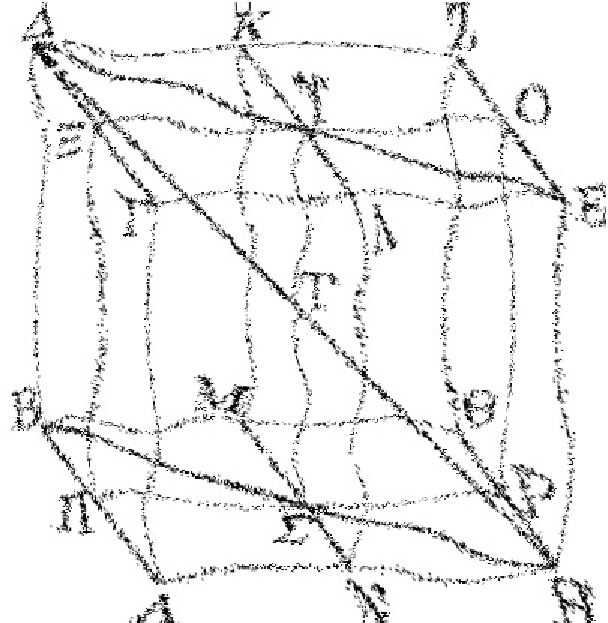
\includegraphics{Book11/front.eps}}
\newpage

%%%%%%%
% Definitions
%%%%%%%
\pdfbookmark[1]{Definitions}{def11}
\pagestyle{fancy}
\cfoot{\gr{\kern -.7pt }}
\lhead{\large\gr{ΣΤΟΙΘΕΙΩΝ \kern -.7pt {11}.}}
\rhead{\large ELEMENTS BOOK 11}
\begin{Parallel}{}{} 
\ParallelLText{
\begin{center}
\large{\gr{<'Οροι}.}
\end{center}\vspace*{-7pt}

\ggn{1}.~\gr{Στερεόν ἐστι τὸ μ\kern -.7pt  ῆκοξ καὶ πλάτοξ καὶ βάθοξ >έθον.}


\ParallelPar
\ggn{2}.~\gr{Στερεοῦ δὲ πέραξ ἐπιφάνεια.}


\ParallelPar
\ggn{3}.~\gr{Εὐθεῖα πρὸξ ἐπίπεδον ὀρθή ἐστιν, <όταν πρὸξ
πάσαξ τὰξ ἁπτομέναξ α\kern -.7pt  ὐτῆξ εὐθείαξ καὶ ο>ύσαξ ἐν τῶ| [ὑποκειμένῳ] ἐπιπέδῳ ὀρθὰξ ποιῆ| γωνίαξ.}

\ParallelPar

\ggn{4}.~\gr{Ἐπίπεδον πρὸξ ἐπίπεδον ὀρθόν ἐστιν, <όταν αἱ τῆ|
κοινῆ| τομ\kern -.7pt  ῆ| τῶν ἐπιπέδων πρὸξ ὀρθὰξ ἀγόμεναι εὐθεῖαι
ἐν ἑνὶ τῶν ἐπιπέδων τῶ| λοιπῶ| ἐπιπέδῳ πρὸξ
ὀρθὰξ >ῶσιν.}

\ParallelPar

\ggn{5}.~\gr{Εὐθείαξ πρὸξ ἐπίπεδον κλίσιξ ἐστίν, <όταν ἀπὸ τοῦ
μετεώρου πέρατοξ τῆξ εὐθείαξ ἐπὶ τὸ ἐπίπεδον κάθετοξ
ἀθθῆ|, καὶ ἀπὸ τοῦ γενομένου σημείου ἐπὶ τὸ ἐν τῶ|
ἐπιπέδῳ πέραξ τῆξ εὐθείαξ εὐθεῖα ἐπιζευθθῆ|, ἡ
περιεθομένη γωνία ὑπὸ τῆξ ἀθθείσηξ καὶ τῆξ ἐφεστώσηξ.}

\ParallelPar

\ggn{6}.~\gr{Ἐπιπέδου πρὸξ ἐπίπεδον κλίσιξ ἐστὶν ἡ περιεθομένη
ὀχεῖα γωνία ὑπὸ τῶν πρὸξ ὀρθὰξ τῆ| κοινῆ| τομ\kern -.7pt  ῆ| ἀγομένων
πρὸξ τῶ| α\kern -.7pt  ὐτῶ| σημείῳ ἐν ἑκατέρῳ τῶν ἐπιπέδων.}

\ParallelPar

\ggn{7}.~\gr{Ἐπίπεδον πρὸξ ἐπίπεδον ὁμοίωξ κεκλίσθαι λέγεται
καὶ <έτερον πρὸξ <έτερον, <όταν αἱ εἰρημέναι τῶν
κλίσεων γωνίαι >ίσαι ἀλλήλαιξ >ῶσιν.}

\ParallelPar

\ggn{8}.~\gr{Παράλληλα ἐπίπεδά ἐστι τὰ ἀσύμπτωτα.}


\ParallelPar
\ggn{9}.~\gr{<'Ομοια στερεὰ σθήματά ἐστι τὰ ὑπὸ ὁμοίων
ἐπιπέδων περιεθόμενα >ίσων τὸ πλῆθοξ.}

\ParallelPar

\ggn{10}.~\gr{>'Ισα δὲ καὶ <όμοια στερεὰ σθήματά ἐστι τὰ ὑπὸ
ὁμοίων ἐπιπέδων περιεθόμενα >ίσων τῶ| πλήθει καὶ τῶ|
μεγέθει.}

\ParallelPar

\ggn{11}.~\gr{Στερεὰ γωνία ἐστὶν ἡ ὑπὸ πλειόνων >ὴ δύο γραμμῶν
ἁπτομένων ἀλλήλων καὶ μ\kern -.7pt  ὴ ἐν τῆ| α\kern -.7pt  ὐτῆ| ἐπιφανείᾳ
οὐσῶν πρὸξ πάσαιξ ταῖξ γραμμαῖξ κλίσιξ. >άλλωξ; στερεὰ γωνία
ἐστὶν ἡ ὑπὸ πλειόνων  >ὴ δύο γωνιῶν ἐπιπέδων
περιεθομένη μ\kern -.5pt  ὴ οὐσῶν ἐν τῶ| α\kern -.3pt  ὐτῶ| ἐπιπέδῳ
πρὸξ ἑνὶ σημείῳ συνισταμένων.}

\ParallelPar

\ggn{12}.~\gr{Πυραμίξ ἐστι σθῆμα στερεὸν ἐπιπέδοιξ περιθόμενον
ἀπὸ ἑνὸξ ἐπιπέδου πρὸξ ἑνὶ σημείῳ συνεστώξ.}

\ParallelPar

\ggn{13}.~\gr{Πρίσμα ἐστὶ σθῆμα στερεὸν ἐπιπέδοιξ περιεχόμενον,
<ῶν δύο τὰ ἀπεναντίον >ίσα τε καὶ <όμοιά ἐστι καὶ
παράλληλα, τὰ δὲ λοιπὰ παραλληλόγραμμα.}

\ParallelPar

\ggn{14}.~\gr{Σφαῖρά ἐστιν, <όταν ἡμικυκλίου μενούσηξ τῆξ διαμέτ\-ρου
περιενεθθὲν τὸ ἡμικύκλιον  εἰξ τὸ α\kern -.7pt  ὐτὸ πάλιν ἀποκατασταθῆ|,
 <όθεν >ήρχατο φέρεσθαι, τὸ περιληφθὲν σθῆμα.}

\ParallelPar
 
\ggn{15}.~\gr{>'Αχων δὲ τῆξ σφαίραξ ἐστὶν ἡ μένουσα εὐθεῖα, περὶ
<ὴν τὸ ἡμικύκλιον στρέφεται.}

\ParallelPar

\ggn{16}.~\gr{Κέντρον δὲ τῆξ σφαίραξ ἐστὶ τὸ α\kern -.7pt  ὐτό, <ὸ καὶ τοῦ
ἡμικυκλίου.}

\ParallelPar

\ggn{17}.~\gr{Διάμετροξ δὲ τῆξ σφαίραξ ἐστὶν εὐθεῖά τιξ διὰ τοῦ
κέντρου ἠγμένη καὶ περατουμένη ἐφ> ἑκάτερα τὰ
μέρη ὑπὸ τῆξ ἐπιφανείαξ τῆξ σφαίραξ.}

\ParallelPar

\ggn{18}.~\gr{Κῶνόξ ἐστιν, <όταν ὀρθογωνίου τριγώνου μενούσηξ μιᾶξ
πλευρᾶξ τῶν περὶ τὴν ὀρθὴν γωνίαν περιενεθθὲν τὸ τρίγωνον εἰξ τὸ 
α\kern -.7pt  ὐτὸ πάλιν ἀποκατασταθῆ|, <όθεν >ήρχατο φέρεσθαι, τὸ περιληφθὲν σθῆμα. κ>ὰν μὲν ἡ μένουσα εὐθεῖα >ίση >ῆ| τῆ| λοιπῆ| [τῆ|] περὶ
τὴν ὀρθὴν περιφερομένῃ, ὀρθογώνιοξ >έσται ὁ κῶνοξ, ἒαν δὲ ἐλάττων, ἀμβλυγώνιοξ, ἒαν δὲ μείζων, ὀχυγώνιοξ.}

\ParallelPar

\ggn{19}.~\gr{>'Αχων δὲ τοῦ κώνου ἐστὶν ἡ μένουσα εὐθεῖα, περὶ
<ὴν τὸ τρίγωνον στρέφεται.}

\ParallelPar

\ggn{20}.~\gr{Βάσιξ δὲ ὁ κύκλοξ ὁ ὑπὸ τῆξ περιφερομένηξ εὐθείαξ  γραφόμενοξ.}


\ParallelPar
\ggn{21}.~\gr{Κύλινδρόξ ἐστιν, <όταν ὀρθογωνίου παραλληλογράμ\-μου μενούσηξ μιᾶξ πλευρᾶξ τῶν περὶ τὴν ὀρθὴν γωνίαν περιενεθθὲν τὸ
παραλληλόγραμμον εἰξ τὸ α\kern -.7pt  ὐτὸ πάλιν ἀποκατασταθῆ|, <όθεν >ήρχατο
φέρεσθαι,
τὸ περιληφθὲν σθῆμα.}

\ParallelPar

\ggn{22}.~\gr{>'Αχων δὲ τοῦ κυλίνδρου ἐστὶν ἡ μένουσα εὐθεῖα,
περὶ <ὴν τὸ παραλληλόγραμμον στρέφεται.}

\ParallelPar

\ggn{23}.~\gr{Βάσειξ δὲ οἱ κύκλοι οἱ ὑπὸ τῶν ἀπεναντίον περιαγομένων
δύο πλευρῶν γραφόμενοι.}

\ParallelPar

\ggn{24}.~\gr{<'Ομοιοι κῶνοι καὶ κύλινδροί εἰσιν, <ῶν ο<ί τε >άχονεξ καὶ
αἱ διάμετροι τῶν βάσεων ἀνάλογόν εἰσιν.}

\ParallelPar

\ggn{25}.~\gr{Κύβοξ ἐστὶ σθῆμα στερεὸν ὑπὸ <ὲχ τετραγώνων >ίσων
περιεχόμενον.}

\ParallelPar

\ggn{26}.~\gr{Ὀκτάεδρόν ἐστὶ σθῆμα στερεὸν ὑπὸ ὀκτὼ τριγώνων 
>ίσων καὶ ἰσοπλεύρων περιεχόμενον.}

\ParallelPar

\ggn{27}.~\gr{Εἰκοσάεδρόν ἐστι σθῆμα στερεὸν ὑπὸ ε>ίκοσι τριγώνων
>ίσων καὶ ἰσοπλεύρων περιεχόμενον.}

\ParallelPar

\ggn{28}.~\gr{Δωδεκάεδρόν ἐστι σθῆμα στερεὸν ὑπὸ δώδεκα πενταγώνων
>ίσων καὶ ἰσοπλεύρων καὶ ἰσογωνίων περιεχόμενον.}}

\ParallelRText{

\ParallelPar
\begin{center}
{\large Definitions}
\end{center}

1.~A solid is a (figure) having length and breadth and depth.

2.~The extremity of a solid (is) a surface.

3.~A straight-line is at right-angles to a plane when it makes right-angles with all of the
straight-lines joined to it which are also in the plane.

4.~A plane is at right-angles to a(nother) plane when (all of) the  straight-lines drawn in one of the planes, at right-angles to the common section
of the planes, are at right-angles to the remaining plane.

5.~The inclination of a straight-line to a plane is the angle contained
by the drawn and standing (straight-lines), when a perpendicular is
lead  to the plane from the end of the (standing) straight-line raised (out of the plane), and a straight-line
is (then) joined from the point (so) generated to the end of the (standing) straight-line (lying) in the plane.

6.~The inclination of a plane to a(nother) plane is the  acute angle
contained by the (straight-lines), (one)  in each of the planes, drawn at right-angles to the common segment
(of the planes), at the same point.

7.~A plane is said to be similarly inclined to a plane,
as another  to  another, when the aforementioned angles
of inclination are equal to one another.

8.~Parallel planes are those which do not meet (one another).

9.~Similar solid figures are those contained by equal numbers of similar
planes (which are similarly arranged).

10.~But equal and similar solid figures are those contained
by similar planes equal in number and in magnitude (which are similarly arranged).

11.~A solid angle is the inclination (constituted) by more than two lines joining one another (at the same point), and
not being in the same surface, to all of the lines. Otherwise,
a solid angle is that contained by more than two plane angles, not being
in the same plane, and constructed at one point.

12.~A pyramid is a solid figure, contained by planes, (which is) constructed from one plane to
one  point.

13.~A prism is a solid figure, contained by planes, of which the two opposite
(planes)
are equal, similar, and parallel, and the remaining (planes are) parallelograms.

14.~A sphere is the figure enclosed when, the diameter of a semicircle remaining (fixed), the semicircle is carried around,
 and  again established at the same (position) from which it began to be moved.
 
15.~And the axis of the sphere is the fixed straight-line about
 which the semicircle is turned.
 
16.~And the center of the sphere is the same as that of the semicircle.

17.~And the diameter of the sphere is any straight-line which is
 drawn through the center and terminated in both directions by
 the surface of the sphere.
 
18.~A cone is the figure enclosed when,  one of the sides of a right-angled triangle about the right-angle remaining (fixed),
  the triangle is carried around, and again established at the
 same (position) from which it began to be moved. And if the
 fixed straight-line is equal to the remaining (straight-line) about the
 right-angle, (which is) carried around, then the cone will be right-angled, and
 if less, obtuse-angled, and if greater, acute-angled.
 
19.~And the axis of the cone is the fixed straight-line about which
 the triangle is turned.
 
20.~And the base (of the cone is) the circle described by the (remaining) straight-line (about the right-angle which is)
 carried around (the axis).
 
21.~A cylinder is the figure enclosed when, one of the sides
 of a right-angled parallelogram about the right-angle remaining (fixed),
 the parallelogram is carried around, and again established at the same
 (position) from which it began to be moved.
 
22.~And the axis of the cylinder is the stationary straight-line about which
 the parallelogram is turned.
 
23.~And the bases (of the cylinder are) the circles described by the
 two opposite sides (which are) carried around.
 
24.~Similar cones and cylinders are those for which the axes and the diameters
 of the bases are proportional.
 
25.~A cube is a solid figure contained by six equal squares.

26.~An octahedron is a solid figure contained by eight equal and
 equilateral triangles.
 
 27.~An icosahedron is a solid figure contained by twenty equal and
 equilateral triangles.
 
28.~A dodecahedron is a solid figure contained by twelve equal,
 equilateral, and equiangular pentagons.}
 \end{Parallel}
 
%%%%
%11.1
%%%%
\pdfbookmark[1]{Proposition 11.1}{pdf11.1}
\begin{Parallel}{}{}
\ParallelLText{
\begin{center}
{\large \ggn{1}.}
\end{center}\vspace*{-7pt}

\gr{Εὐθείαξ γραμμ\kern -.7pt  ῆξ μέροξ μέν τι οὐκ >έστιν ἐν τῶ| ὑποκειμένῳ
ἐπιπέδῳ, μέροξ δέ τι ἐν μετεωροτέρῳ.}

\gr{Εἰ γὰρ δυνατόν, εὐθείαξ γραμμ\kern -.7pt  ῆξ τῆξ ΑΒΓ μέροξ
μέν τι τὸ ΑΒ >έστω ἐν τῶ| ὑποκειμένῳ ἐπιπέδῳ,
μέροξ δέ τι τὸ ΒΓ ἐν μετεωροτέρῳ.}

\gr{>'Εσται δή τιξ τῆ| ΑΒ συνvεθὴξ εὐθεῖα ἐπ> εὐθείαξ ἐν
τῶ| ὑποκειμένῳ ἐπιπέδῳ. >έστω ἡ ΒΔ; δύο >άρα εὐθειῶν
τῶν ΑΒΓ, ΑΒΔ κοινὸν τμ\kern -.7pt  ῆμά ἐστιν ἡ ΑΒ; <όπερ ἐστὶν
ἀδύνατον, ἐπειδήπερ ἒαν κέντρῳ τῶ| Β καὶ διαστήματι
τῶ| ΑΒ κύκλον γράψωμεν, αἱ διάμετροι ἀνίσουξ ἀπολήψονται
τοῦ κύκλου περιφερείαξ.}\\

\epsfysize=2.5in
\centerline{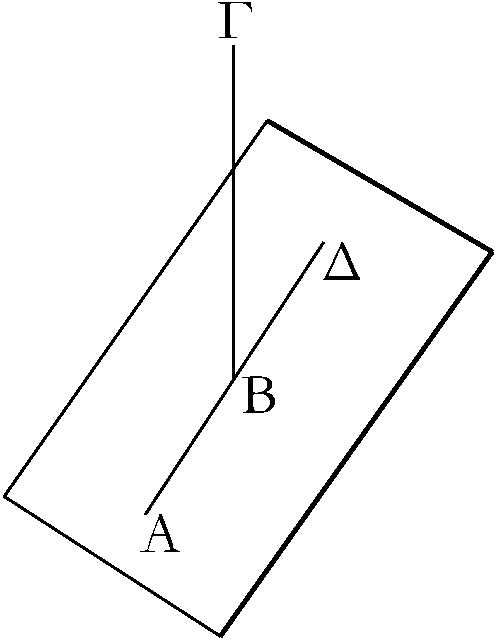
\includegraphics{Book11/fig01g.eps}}

\gr{Εὐθείαξ >άρα γραμμ\kern -.7pt  ῆξ μέροξ μέν τι οὐκ >έστιν ἐν τῶ| ὑποκειμένῳ ἐπιπέδῳ, τὸ δὲ ἐν μετεωροτέρῳ; <όπερ
>έδει δεῖχαι.}}

\ParallelRText{
\begin{center}
{\large Proposition 1}$^\dag$
\end{center}

Some part of a straight-line cannot be in a reference
plane, and some part in a more elevated (plane).

For, if possible, let some part, $AB$, of the straight-line $ABC$ be
in a reference plane, and some part, $BC$, in a more elevated (plane).

In the reference plane, there will be some straight-line continuous with, and straight-on to, $AB$.$^\ddag$ Let it be $BD$. Thus, $AB$ is a common
segment of the two (different) straight-lines $ABC$ and $ABD$. The
very thing is impossible, inasmuch as if we draw a circle with center $B$
and radius $AB$ then the diameters ($ABD$ and $ABC$) will cut off unequal circumferences
of the circle.

\epsfysize=2.5in
\centerline{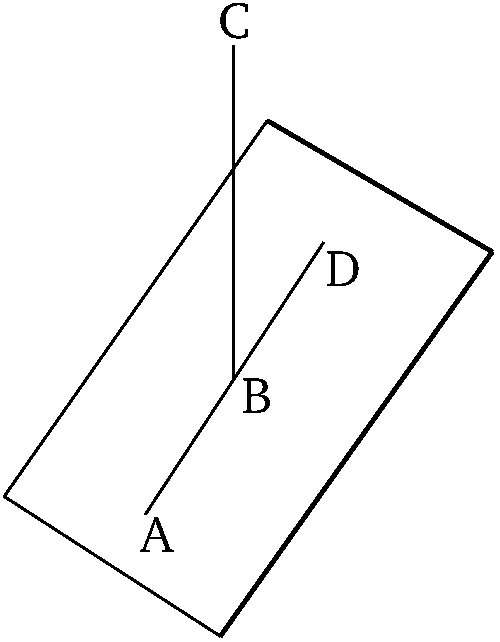
\includegraphics{Book11/fig01e.eps}}

Thus, some part of a straight-line cannot be in a reference
plane, and (some part) in a more elevated (plane). (Which is) the very thing it
was required to show.}
\end{Parallel}
{\footnotesize\noindent$^\dag$ The proofs of the first three propositions in this book are not at all rigorous. Hence,  these three propositions should properly be regarded as additional axioms.}\\
{\footnotesize\noindent$^\ddag$ This assumption essentially presupposes the validity of the proposition under discussion.} 

%%%%
%11.2
%%%%
\pdfbookmark[1]{Proposition 11.2}{pdf11.2}
\begin{Parallel}{}{}
\ParallelLText{
\begin{center}
{\large \ggn{2}.}
\end{center}\vspace*{-7pt}

\gr{Ἐὰν δύο εὐθεῖαι τέμνωσιν ἀλλήλαξ, ἐν ἑνί εἰσιν
ἐπιπέδῳ, καὶ πᾶν τρίγωνον ἐν ἑνί ἐστιν ἐπιπέδῳ.}\\

\epsfysize=2.in
\centerline{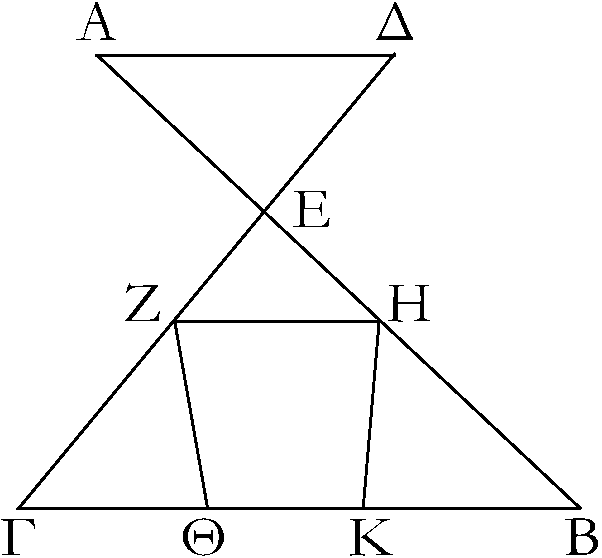
\includegraphics{Book11/fig02g.eps}}

\gr{Δύο γὰρ εὐθεῖαι αἱ ΑΒ, ΓΔ τεμνέτωσαν ἀλλήλαξ κατὰ τὸ Ε
σημεῖον. λέγω, <ότι αἱ ΑΒ, ΓΔ ἐν ἑνί εἰσιν ἐπιπέδῳ,
καὶ  πᾶν τρίγωνον ἐν ἑνί ἐστιν ἐπιπέδῳ.}

\gr{Εἰλήφθω γὰρ ἐπὶ τῶν ΕΓ, ΕΒ τυθόντα σημεῖα τὰ Ζ, Η,
καὶ ἐπεζεύθθωσαν αἱ ΓΒ, ΖΗ, καὶ διήθθωσαν αἱ ΖJ, ΗΚ;
λέγω πρῶτον, <ότι τὸ ΕΓΒ τρίγωνον ἐν ἑνί ἐστιν ἐπιπέδῳ.
εἰ γάρ ἐστι τοῦ ΕΓΒ τριγώνου μέροξ >ήτοι τὸ ΖJΓ >ὴ τὸ ΗΒΚ
ἐν τῶ| ὑποκειμένῳ
 [ἐπιπέδῳ], τὸ δὲ λοιπὸν ἐν >άλλῳ,
>έσται καὶ μιᾶξ τῶν ΕΓ, ΕΒ εὐθειῶν μέροξ μέν τι ἐν τῶ|
ὑποκειμένῳ ἐπιπέδῳ, τὸ δὲ ἐν αλλῳ. εἰ δὲ τοῦ ΕΓΒ
τριγώνου τὸ ΖΓΒΗ μέροξ >ῆ| ἐν τῶ| ὑποκειμένῳ
ἐπιπέδῳ, τὸ δὲ λοιπὸν ἐν >άλλῳ, >έσται καὶ ἀμφοτέρων τῶν
ΕΓ, ΕΒ εὐθειῶν μέροξ μέν τι ἐν τῶ| ὑποκειμένῳ
ἐπιπέδῳ, τὸ δὲ ἐν >άλλω; <όπερ >άτοπον ἐδείθθη. τὸ >άρα
ΕΓΒ τρίγωνον ἐν ἑνί ἐστιν ἐπιπέδῳ. ἐν <ῶ| δέ ἐστι
τὸ ΕΓΒ τρίγωνον, ἐν τούτῳ καὶ ἑκατέρα τῶν ΕΓ,
ΕΒ, ἐν <ῶ| δὲ ἑκατέρα τῶν ΕΓ, ΕΒ, ἐν τούτῳ καὶ
αἱ ΑΒ, ΓΔ. αἱ ΑΒ, ΓΔ >άρα εὐθεῖαι ἐν ἑνί εἰσιν
ἐπιπέδῳ, καὶ πᾶν τρίγωνον ἐν ἑνί ἐστιν ἐπιπέδῳ;
<όπερ >έδει δεῖχαι.}}

\ParallelRText{
\begin{center}
{\large Proposition 2}
\end{center}

If two straight-lines cut one another then they are
in one plane, and every triangle (formed using segments of
both lines) is in one plane.

\epsfysize=2.in
\centerline{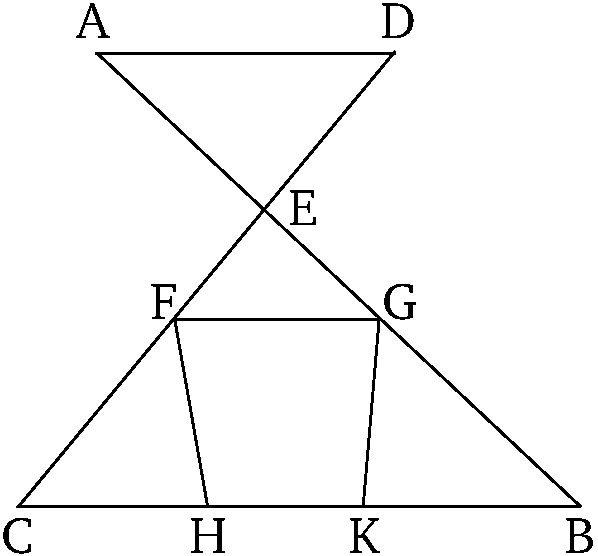
\includegraphics{Book11/fig02e.eps}}

For let the two straight-lines $AB$ and $CD$ have cut one another at point
$E$. I say that $AB$ and $CD$ are in one plane, and that every
triangle (formed using segments of both lines) is in one plane.

For let the random points $F$ and $G$ be taken on $EC$ and
$EB$ (respectively). And let $CB$ and $FG$ be joined, and let
$FH$ and $GK$ be drawn across. I say, first of all, that triangle
$ECB$ is in one (reference) plane. For if part of triangle $ECB$, either $FHC$ or
$GBK$, is in the reference [plane], and the remainder in a different (plane)
then a part  of one the straight-lines $EC$ and $EB$
will also be in the reference plane, and (a part) in a different (plane).
And if the part $FCBG$ of triangle $ECB$ is in the reference plane, and
the remainder in a different (plane) then parts of both of the straight-lines
$EC$ and $EB$ will also be in  the reference plane, and (parts) in a
different (plane). The very thing was shown to be absurb [Prop.~11.1]. Thus, triangle $ECB$ is in
one plane. And in whichever (plane) triangle $ECB$ is (found),  in that (plane) $EC$ and $EB$ (will) each also (be found). And in whichever (plane) 
 $EC$
and $EB$ (are) each (found), in that (plane) $AB$ and $CD$ (will) also (be found)  [Prop.~11.1]. Thus, the straight-lines $AB$ and
$CD$ are in one plane, and every triangle (formed using segments of
both lines) is in one plane. (Which is) the very thing it was required to
show.}
\end{Parallel}

%%%%
%11.3
%%%%
\pdfbookmark[1]{Proposition 11.3}{pdf11.3}
\begin{Parallel}{}{}
\ParallelLText{
\begin{center}
{\large \ggn{3}.}
\end{center}\vspace*{-7pt}

\gr{Ἐὰν δύο ἐπίπεδα τεμνῆ| >άλληλα, ἡ κοινὴ α\kern -.7pt  ὐτῶν τομ\kern -.7pt  ὴ εὐθεῖά ἐστιν.}

\epsfysize=1.8in
\centerline{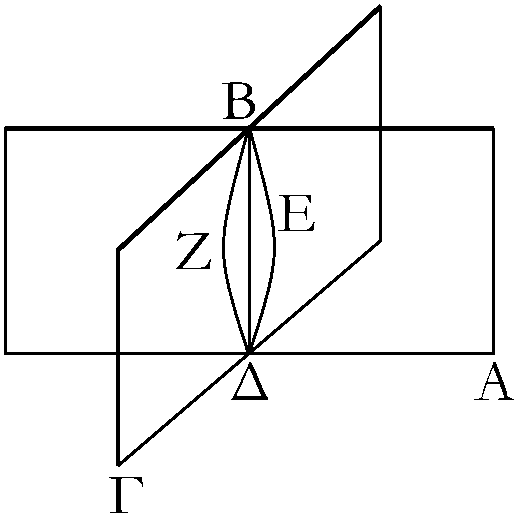
\includegraphics{Book11/fig03g.eps}}

\gr{Δύο γὰρ ἐπίπεδα τὰ ΑΒ, ΒΓ τεμνέτω >άλληλα, κοινὴ δὲ α\kern -.7pt  ὐτῶν
τομ\kern -.7pt  ὴ >έστω ἡ ΔΒ γραμμ\kern -.5pt  ή; λέγω, <ότι ἡ ΔΒ γραμμ\kern -.3pt  ὴ εὐθεῖά
ἐστιν.}

\gr{Εἰ γὰρ μ\kern -.7pt  ή, ἐπεζεύθθω ἀπὸ τοῦ Δ ἐπὶ τὸ Β ἐν
μὲν τῶ| ΑΒ ἐπιπέδῳ εὐθεῖα ἡ ΔΕΒ, ἐν δὲ τῶ|
ΒΓ ἐπιπέδῳ εὐθεῖα ἡ ΔΖΒ. >έσται δὴ δύο εὐθειῶν
τῶν ΔΕΒ, ΔΖΒ τὰ α\kern -.7pt  ὐτὰ πέρατα, καὶ περιέχουσι δηλαδὴ
θωρίον; <όπερ >άτοπον. ο>ύκ >άρα αἰ ΔΕΒ, ΔΖΒ εὐθεῖαί
εἰσιν. ὁμοίωξ δὴ δείχομεν, <ότι οὐδὲ >άλλη τιξ ἀπὸ
τοῦ Δ ἐπὶ τὸ Β ἐπιζευγνυμένη εὐθεῖα >έσται πλὴν
τῆξ ΔΒ κοινῆξ τομ\kern -.5pt  ῆξ τῶν ΑΒ, ΒΓ ἐπιπέδων.}

\gr{Ἐὰν >άρα δύο ἐπίπεδα τέμνῃ >άλληλα, ἡ κοινὴ α\kern -.7pt  ὐτῶν
τομ\kern -.7pt  ὴ εὐθεῖά ἐστιν; <όπερ >έδει δεῖχαι.}}

\ParallelRText{
\begin{center}
{\large Proposition 3}
\end{center}

If two planes cut one another then their common
section is a straight-line.

\epsfysize=1.8in
\centerline{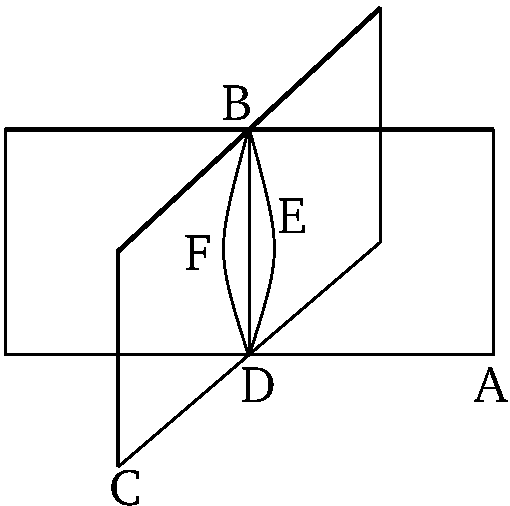
\includegraphics{Book11/fig03e.eps}}

For let the two planes $AB$ and $BC$ cut one another, and let their
common section be the line $DB$. I say that the line $DB$ is straight.

For, if not,  let the straight-line $DEB$ be joined from $D$ to $B$
in the plane $AB$, and the straight-line $DFB$ in the plane $BC$. 
So two straight-lines, $DEB$ and $DFB$, will have the same ends, and
they will clearly enclose an area. The very thing (is) absurd. Thus,
$DEB$ and $DFB$ are not straight-lines.  So, similarly, we can show
than no other straight-line  can be joined from $D$ to $B$  except $DB$, the common section of the planes $AB$ and $BC$.

Thus, if  two planes cut one another then their common
section is a straight-line. (Which is) the very thing it was required to
show.}
\end{Parallel}

%%%%
%11.4
%%%%
\pdfbookmark[1]{Proposition 11.4}{pdf11.4}
\begin{Parallel}{}{}
\ParallelLText{
\begin{center}
{\large \ggn{4}.}
\end{center}\vspace*{-7pt}

\gr{Ἐὰν εὐθεῖα δύο εὐθείαιξ  τεμνούσαιξ ἀλλήλαξ πρὸξ ὀρθὰξ ἐπὶ
τῆξ κοινῆξ τομ\kern -.7pt  ῆξ ἐπισταθῆ|, καὶ τῶ| δι> α\kern -.7pt  ὐτῶν ἐπιπέδῳ
πρὸξ ὀρθὰξ >έσται.}

\gr{Εὐθεῖα γάρ τιξ ἡ ΕΖ δύο εὐθείαιξ ταῖξ ΑΒ, ΓΔ
τεμνούσαιξ ἀλλήλαξ κατὰ τὸ Ε σημεῖον ἀπὸ τοῦ
Ε πρὸξ ὀρθὰξ ἐφεστάτω; λέγω, <ότι ἡ ΕΖ καὶ τῶ|
διὰ τῶν ΑΒ, ΓΔ ἐπιπέδῳ πρὸξ ὀρθάξ ἐστιν.}

\gr{Ἀπειλήφθωσαν γὰρ αἱ ΑΕ, ΕΒ, ΓΕ, ΕΔ >ίσαι ἀλλήλαιξ, καὶ
διήθθω τιξ διὰ τοῦ Ε, ὡξ >έτυθεν, ἡ ΗΕJ, καὶ ἐπεζεύθθωσαν
αἱ ΑΔ, ΓΒ, καὶ >έτι ἀπὸ τυθόντοξ τοῦ Ζ ἐπεζεύθθωσαν
αἱ ΖΑ, ΖΗ, ΖΔ, ΖΓ, ΖJ, ΖΒ.}\\~\\~\\

\epsfysize=2.in
\centerline{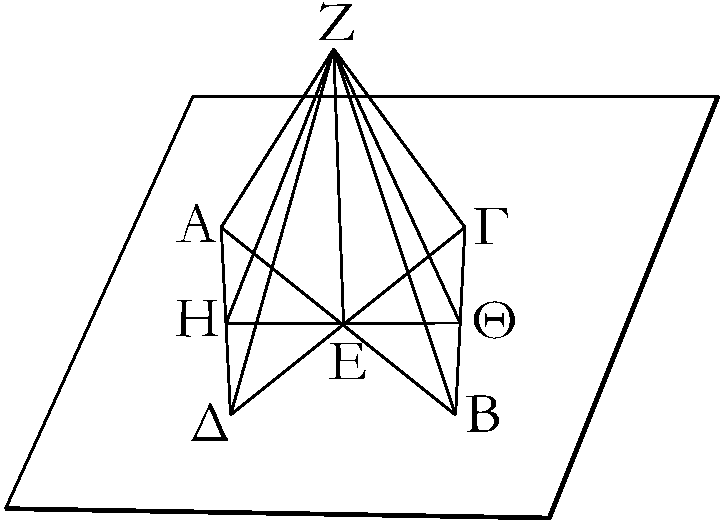
\includegraphics{Book11/fig04g.eps}}

\gr{Καὶ ἐπεὶ δύο αἱ ΑΕ, ΕΔ δυσὶ ταῖξ
ΓΕ, ΕΒ >ίσαι εἰσὶ καὶ γωνίαξ >ίσαξ περιέθουσιν, βάσιξ >άρα
ἡ ΑΔ βάσει τῆ| ΓΒ >ίση ἐστίν, καὶ τὸ ΑΕΔ τρίγωνον τῶ| ΓΕΒ
τριγώνῳ >ίσον >έσται; <ώστε καὶ γωνία ἡ ὑπὸ ΔΑΕ γωνίᾳ
τῆ| ὑπὸ ΕΒΓ >ίση [ἐστίν]. >έστι δὲ καὶ ἡ ὑπὸ ΑΕΗ γωνία
τῆ| ὑπὸ ΒΕJ >ίση. δύο δὴ τρίγωνά ἐστι τὰ ΑΗΕ, ΒΕJ τὰξ
δύο γωνίαξ δυσὶ γωνίαιξ >ίσαξ >έθοντα ἑκατέραν ἑκατέρᾳ καὶ
μίαν πλευρὰν μιᾶ| πλευρᾶ| >ίσην τὴν πρὸξ ταῖξ >ίσαιξ γωνίαιξ
τὴν ΑΕ τῆ| ΕΒ; καὶ τὰξ λοιπὰξ >άρα πλευρὰξ ταῖξ λοιπαῖξ
πλευραῖξ >ίσαξ <έχουσιν. >ίση >άρα ἡ μὲν ΗΕ τῆ| ΕJ, ἡ δὲ
ΑΗ τῆ| ΒJ. καὶ ἐπεὶ >ίση ἐστὶν ἡ ΑΕ τῆ| ΕΒ, κοινὴ
δὲ καὶ πρὸξ ὀρθὰξ ἡ ΖΕ, βάσιξ >άρα ἡ ΖΑ βάσει τῆ| ΖΒ
ἐστιν >ίση. διὰ τὰ α\kern -.7pt  ὐτὰ δὴ καὶ ἡ ΖΓ τῆ| ΖΔ ἐστιν >ίση.
καὶ ἐπεὶ >ίση ἐστὶν ἡ ΑΔ τῆ| ΓΒ, >έστι
δὲ καὶ ἡ ΖΑ τῆ| ΖΒ >ίση, δύο δὴ αἱ ΖΑ, ΑΔ δυσὶ ταῖξ
ΖΒ, ΒΓ >ίσαι εἰσὶν ἑκατέρα ἑκατέρᾳ; καὶ βάσιξ ἡ ΖΔ
βάσει τῆ| ΖΓ ἐδείθθη >ίση; καὶ γωνία >άρα
ἡ ὑπὸ ΖΑΔ γωνίᾳ τῆ| ὑπὸ ΖΒΓ >ίση ἐστίν. καὶ
ἐπεὶ πάλιν ἐδείθθη ἡ ΑΗ τῆ| ΒJ >ίση, ἀλλὰ μ\kern -.7pt  ὴν καὶ
ἡ ΖΑ τῆ| ΖΒ >ίση, δύο δὴ αἱ ΖΑ, ΑΗ δυσὶ ταῖξ
ΖΒ, ΒJ >ίσαι εἰσίν. καὶ γωνία ἡ ὑπὸ ΖΑΗ ἐδείθθη
>ίση τῆ| ὑπὸ ΖΒJ; βάσιξ >άρα ἡ ΖΗ βάσει τῆ| ΖJ ἐστιν >ίση. καὶ
ἐπεὶ πάλιν >ίση ἐδείθθη ἡ ΗΕ τῆ| ΕJ, κοινὴ δὲ ἡ ΕΖ,
δύο δὴ αἱ ΗΕ, ΕΖ δυσὶ ταῖξ JΕ, ΕΖ >ίσαι εἰσίν; καὶ
βάσιξ ἡ ΖΗ βάσει τῆ| ΖJ >ίση; γωνία >άρα ἡ ὑπὸ ΗΕΖ γωνίᾳ
τῆ| ὑπὸ JΕΖ >ίση ἐστίν. ὀρθὴ >άρα ἑκατέρα τῶν ὑπὸ
ΗΕΖ, JΕΖ γωνιῶν.  ἡ ΖΕ >άρα πρὸξ τὴν  ΗJ τυθόντωξ διὰ
τοῦ Ε ἀθθεῖσαν ὀρθή ἐστιν. ὁμοίωξ δὴ δείχομεν,
<ότι ἡ ΖΕ καὶ πρὸξ πάσαξ τὰξ ἁπτομέναξ α\kern -.5pt  ὐτῆξ
εὐθείαξ καὶ ο>ύσαξ ἐν τῶ| ὑποκειμένῳ ἐπιπέδῳ
ὀρθὰξ ποιήσει γωνίαξ. εὐθεῖα δὲ πρὸξ ἐπίπεδον
ὀρθή ἐστιν, <όταν πρὸξ πάσαξ τὰξ ἁπτομέναξ α\kern -.3pt  ὐτῆξ
εὐθείαξ καὶ ο>ύσαξ ἐν τῶ| α\kern -.7pt  ὐτῶ| ἐπιπέδῳ ὀρθὰξ ποιῆ|
γωνίαξ; ἡ ΖΕ >άρα τῶ| ὑποκειμένῳ ἐπιπέδῳ πρὸξ ὀρθάξ
ἐστιν. τὸ δὲ ὑποκείμενον ἐπίπεδόν ἐστι τὸ διὰ τῶν
ΑΒ, ΓΔ εὐθειῶν. ἡ ΖΕ >άρα πρὸξ ὀρθάξ ἐστι τῶ| διὰ
τῶν ΑΒ, ΓΔ ἐπιπέδῳ.}

\gr{Ἐὰν >άρα εὐθεῖα δύο εὐθείαιξ  τεμνούσαιξ ἀλλήλαξ πρὸξ ὀρθὰξ ἐπὶ
τῆξ κοινῆξ τομ\kern -.7pt  ῆξ ἐπισταθῆ|, καὶ τῶ| δι> α\kern -.7pt  ὐτῶν ἐπιπέδῳ
πρὸξ ὀρθὰξ >έσται; <όπερ >έδει δεῖχαι.}}

\ParallelRText{
\begin{center}
{\large Proposition 4}
\end{center}

If a straight-line is set up at right-angles to two straight-lines cutting one another, at the common  point of section,  then it will also be
at right-angles to the plane (passing) through them (both).

For let some straight-line $EF$ have (been) set up  at right-angles to two
straight-lines, $AB$ and $CD$, cutting one another at point $E$, at $E$. I say that
$EF$ is also at right-angles to the plane (passing) through $AB$ and $CD$.

For let $AE$, $EB$, $CE$ and $ED$ be cut off from (the two straight-lines
so as to be) equal to one another. And let $GEH$ be drawn, at random,
through $E$ (in the plane passing through $AB$ and $CD$). And let $AD$ and $CB$ be joined. And, furthermore,
let $FA$, $FG$, $FD$, $FC$, $FH$, and $FB$ be joined
from the random (point) $F$ (on $EF$).

\epsfysize=2.in
\centerline{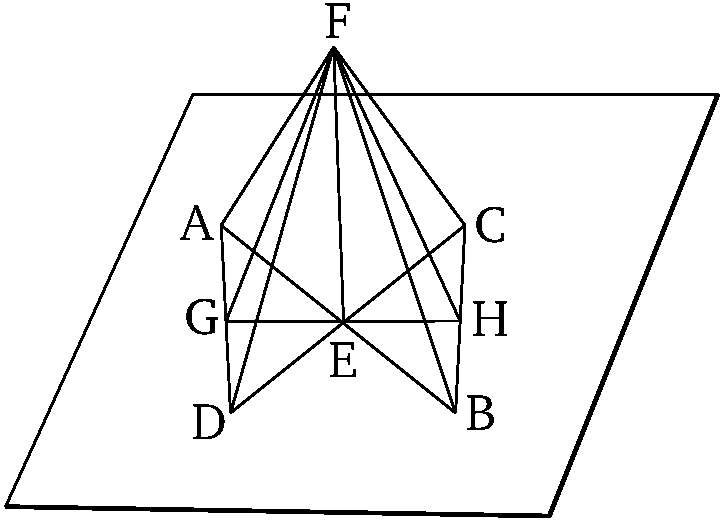
\includegraphics{Book11/fig04e.eps}}

For since the two (straight-lines) $AE$ and $ED$ are equal to the two (straight-lines) $CE$ and $EB$, and they  enclose equal angles [Prop.~1.15], the base $AD$ is thus equal to the
base $CB$, and triangle $AED$ will be equal to triangle $CEB$ [Prop.~1.4]. Hence, the angle $DAE$ [is] equal to
the angle $EBC$. And the angle $AEG$ (is)  also equal to the angle
$BEH$ [Prop.~1.15]. So $AGE$ and $BEH$
are two triangles having two angles equal to two angles, respectively, and
one side equal to one side---(namely), those by the equal angles, $AE$ and $EB$. Thus, they will also have the remaining sides equal to the remaining
sides [Prop.~1.26]. Thus, $GE$ (is) equal to $EH$, 
and $AG$ to $BH$. And since $AE$ is equal to $EB$, and $FE$ is
common and at right-angles, the base $FA$ is thus equal to the base $FB$ [Prop.~1.4]. So, for the same (reasons), $FC$ is also
equal to $FD$. And since $AD$ is equal to $CB$, and $FA$ is also equal to
$FB$, the two (straight-lines) $FA$ and $AD$ are equal to the
two (straight-lines) $FB$ and $BC$, respectively. And the base $FD$
was shown (to be) equal to the base $FC$. Thus, the angle $FAD$ is also
equal to the angle $FBC$ [Prop.~1.8]. And, again,
since $AG$ was shown (to be) equal to $BH$, but $FA$ (is) also equal to
$FB$, the two (straight-lines) $FA$ and $AG$ are equal to the
two (straight-lines) $FB$ and $BH$ (respectively). And the angle $FAG$
was shown (to be) equal to the angle $FBH$. Thus, the base $FG$ is equal
to the base $FH$ [Prop.~1.4]. And, again, since
$GE$ was shown (to be) equal to $EH$, and $EF$ (is) common, the two
(straight-lines) $GE$ and $EF$ are equal to the two (straight-lines)
$HE$ and $EF$ (respectively). And the base $FG$
(is) equal to the base $FH$. Thus, the angle $GEF$ is equal to the
angle $HEF$ [Prop.~1.8]. Each of the
angles $GEF$ and $HEF$ (are) thus right-angles [Def.~1.10]. Thus, $FE$ is
at right-angles to $GH$, which was drawn at random through $E$ (in the reference plane passing though $AB$ and $AC$). So, similarly, we can show that
$FE$ will make right-angles with all straight-lines joined to it which are in the reference plane. And a straight-line is at right-angles
to a plane when it makes right-angles with all straight-lines joined to
it which are in the plane [Def.~11.3]. Thus,
$FE$ is at right-angles to the reference plane. And the reference plane
is that (passing) through the straight-lines $AB$ and $CD$. Thus,
$FE$ is at right-angles to the plane (passing) through $AB$ and
$CD$.

Thus, if a straight-line is set up at right-angles to two straight-lines cutting one another, at the common point of section, then it will also be
at right-angles to the plane (passing) through them (both). (Which is)
the very thing it was required to show.}
\end{Parallel}

%%%%
%11.5
%%%%
\pdfbookmark[1]{Proposition 11.5}{pdf11.5}
\begin{Parallel}{}{}
\ParallelLText{
\begin{center}
{\large \ggn{5}.}
\end{center}\vspace*{-7pt}

\gr{Ἐὰν εὐθεῖα τρισὶν εὐθείαιξ ἁπτομέναιξ ἀλλήλων πρὸξ ὀρθὰξ
ἐπὶ τῆξ κοινῆξ τομ\kern -.7pt  ῆξ ἐπισταθῆ|, αἱ τρεῖξ εὐθεῖαι ἐν ἑνί
εἰσιν ἐπιπέδῳ.}

\epsfysize=2.in
\centerline{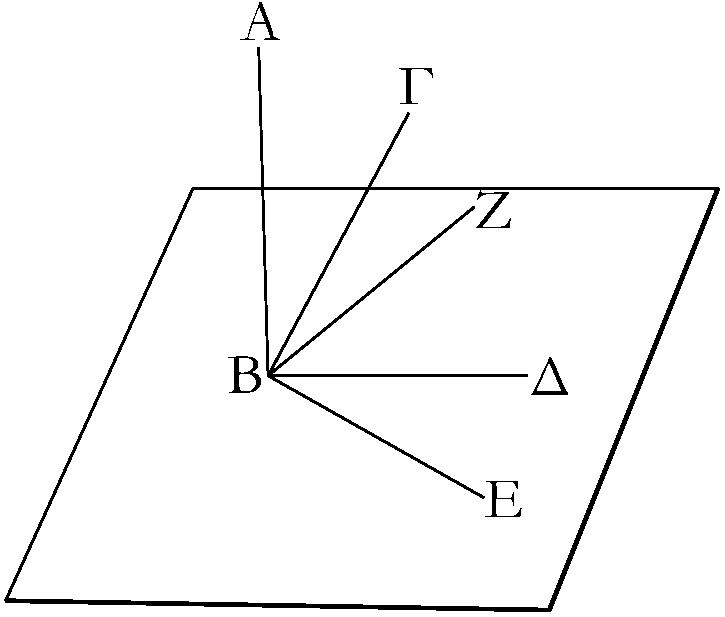
\includegraphics{Book11/fig05g.eps}}

\gr{Εὐθεῖα γάρ τιξ ἡ ΑΒ τρισὶν εὐθείαιξ ταῖξ ΒΓ, ΒΔ, ΒΕ πρὸξ ὀρθὰξ
ἐπὶ τῆξ κατὰ τὸ Β ἁφῆξ ἐφεστάτω; λέγω, <ότι αἱ ΒΓ, ΒΔ, ΒΕ ἐν
ἑνί εἰσιν ἐπιπέδῳ.}

\gr{μ\kern -.7pt  ὴ γάρ, ἀλλ> εἰ δυνατόν, >έστωσαν αἱ μὲν ΒΔ, ΒΕ ἐν τῶ| ὑποκειμένῳ ἐπιπέδῳ, ἡ δὲ ΒΓ ἐν μετεωροτέρῳ, καὶ ἐκβεβλήσθω
τὸ δὶα τῶν ΑΒ, ΒΓ ἐπίπεδον; κοινὴν δὴ τομ\kern -.7pt  ὴν ποιήσει ἐν τῶ|
ὑποκειμένῳ ἐπιπέδῳ εὐθεῖαν. ποιείτω τὴν ΒΖ. ἐν ἑνὶ >άρα
εἰσὶν ἐπιπέδῳ τῶ| διηγμένῳ διὰ τῶν ΑΒ, ΒΓ αἱ τρεῖξ
εὐθεῖαι αἱ ΑΒ, ΒΓ, ΒΖ. καὶ ἐπεὶ ἡ ΑΒ ὀρθή ἐστι πρὸξ
ἑκατέραν τῶν ΒΔ, ΒΕ, καὶ τῶ| διὰ τῶν ΒΔ, ΒΕ
>άρα ἐπιπέδῳ ὀρθή ἐστιν ἡ ΑΒ. τὸ δὲ διὰ τῶν ΒΔ, ΒΕ ἐπίπεδον
τὸ ὑποκείμενόν ἐστιν; ἡ ΑΒ >άρα ὀρθή ἐστι πρὸξ τὸ ὑποκείμενον
ἐπίπεδον. <ώστε καὶ πρὸξ πάσαξ τὰξ ἁπτομέναξ α\kern -.5pt  ὐτῆξ εὐθείαξ
καὶ ο>ύσαξ ἐν τῶ| ὑποκειμένῳ ἐπιπέδῳ ὀρθὰξ ποιήσει γωνίαξ
ἡ ΑΒ. <άπτεται δὲ α\kern -.3pt  ὐτῆξ ἡ ΒΖ ο~ὐσα ἐν τῶ| ὑποκειμένῳ
ἐπιπέδῳ; ἡ >άρα ὑπὸ ΑΒΖ γωνία ὀρθή ἐστιν. ὑπόκειται
δὲ καὶ ἡ ὑπὸ ΑΒΓ ὀρθή; >ίση >άρα ἡ ὑπὸ ΑΒΖ γωνία τῆ|
ὑπὸ ΑΒΓ. καί εἰσιν ἐν ἑνὶ ἐπιπέδῳ; <όπερ
ἐστὶν ἀδύνατον. οὐκ >άρα ἡ ΒΓ εὐθεῖα ἐν μετεωροτέρῳ ἐστὶν
ἐπιπέδῳ; αἱ τρεῖξ >άρα εὐθεῖαι αἱ ΒΓ, ΒΔ, ΒΕ ἐν ἑνί
εἰσιν ἐπιπέδῳ.}

\gr{Ἐὰν >άρα  εὐθεῖα τρισὶν εὐθείαιξ ἁπτομέναιξ ἀλλήλων ἐπὶ τῆξ
ἁφῆξ πρὸξ ὀρθὰξ
ἐπισταθῆ|, αἱ τρεῖξ εὐθεῖαι ἐν ἑνί
εἰσιν ἐπιπέδῳ; <όπερ >έδει δεῖχαι.}}

\ParallelRText{
\begin{center}
{\large Proposition 5}
\end{center}

If a straight-line is set up at right-angles to three straight-lines cutting one another, at the common
point of section, then the three straight-lines are in one plane.

\epsfysize=2.in
\centerline{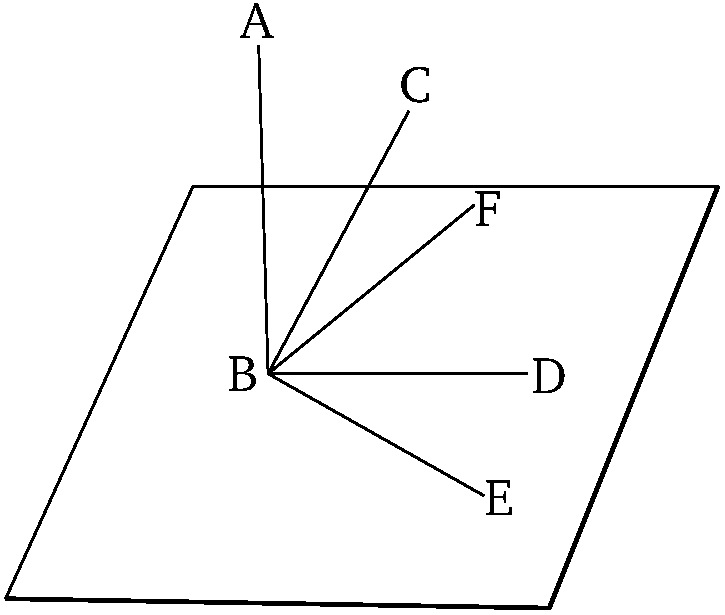
\includegraphics{Book11/fig05e.eps}}

For let some straight-line $AB$ be set up at right-angles
to three straight-lines $BC$, $BD$, and $BE$, at the (common) point of
section $B$. I say that $BC$, $BD$, and $BE$ are in  one plane.

For (if) not, and if possible, let $BD$ and $BE$ be in the reference plane,
and $BC$ in a more elevated (plane).  And let the plane through $AB$ and
$BC$ be produced. So it will make a straight-line as a
common section with the reference plane [Def.~11.3]. 
Let it make $BF$. Thus, the three straight-lines $AB$, $BC$, and $BF$
are in one plane---(namely), that drawn through $AB$ and $BC$. And since
$AB$ is at right-angles to each of $BD$ and $BE$, $AB$ is thus also at right-angles to the plane (passing) through $BD$ and $BE$ [Prop.~11.4]. And the plane (passing)
through $BD$ and $BE$ is the reference plane. Thus, $AB$ is at
right-angles to the reference plane. Hence, $AB$ will also make right-angles
with all straight-lines joined to it which are also in the reference plane [Def.~11.3].
And $BF$, which is in the reference plane, is joined to  it. Thus, the angle
$ABF$ is a right-angle. And $ABC$ was also assumed to be a right-angle.
Thus, angle $ABF$ (is) equal to $ABC$. And they are in one
plane. The very thing is impossible. Thus, $BC$ is not in a more elevated
plane. Thus, the three straight-lines $BC$, $BD$, and $BE$ are in one plane.

Thus, if a straight-line is set up at right-angles to three straight-lines cutting
one another, at the (common) point of section, then the three straight-lines
are in one plane. (Which is) the very thing it was required to show.}
\end{Parallel}

%%%%
%11.6
%%%%
\pdfbookmark[1]{Proposition 11.6}{pdf11.6}
\begin{Parallel}{}{}
\ParallelLText{
\begin{center}
{\large \ggn{6}.}
\end{center}\vspace*{-7pt}

\gr{Ἐὰν δύο εὐθεῖαι τῶ| α\kern -.7pt  ὐτῶ| ἐπιπέδῳ πρὸξ ὀρθὰξ >ῶσιν,
παράλληλοι >έσονται αἱ εὐθεῖαι.}

\epsfysize=2.in
\centerline{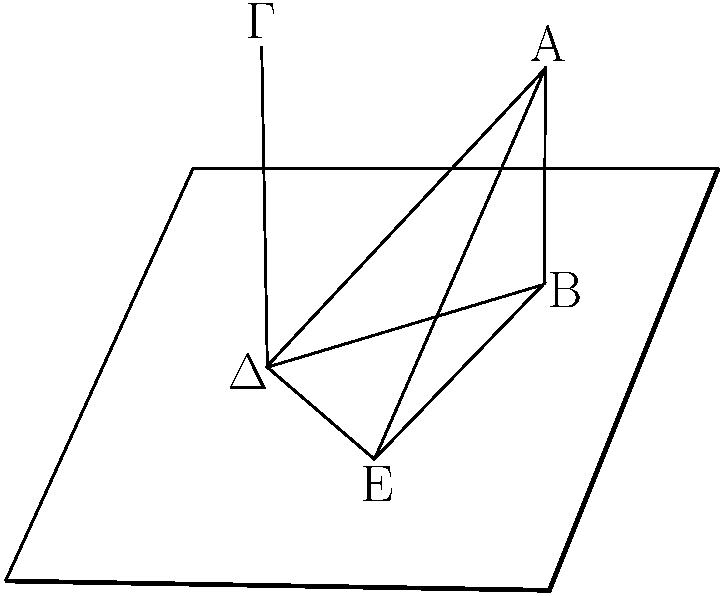
\includegraphics{Book11/fig06g.eps}}

\gr{Δύο γὰρ εὐθεῖαι αἱ ΑΒ, ΓΔ τῶ| ὑποκειμένῳ ἐπιπέδῳ πρὸξ
ὀρθὰξ >έστωσαν; λέγω, <ότι παράλληλόξ ἐστιν ἡ ΑΒ τῆ| ΓΔ.}

\gr{Συμβαλλέτωσαν γὰρ τῶ| ὑποκειμένῳ ἐπιπέδῳ κατὰ
τὰ Β, Δ σημεῖα, καὶ ἐπεζεύθθω ἡ ΒΔ εὐθεῖα, καὶ >ήθθω
τῆ| ΒΔ πρὸξ ὀρθὰξ ἐν τῶ| ὑποκειμένῳ ἐπιπέδῳ
ἡ ΔΕ, καὶ κείσθω τῆ| ΑΒ >ίση ἡ ΔΕ, καὶ ἐπεζεύθθωσαν αἱ
ΒΕ, ΑΕ, ΑΔ.}

\gr{Καὶ ἐπεὶ ἡ ΑΒ ὀρθή ἐστι πρὸξ τὸ ὑποκείμενον ἐπίπεδον,
καὶ πρὸξ πάσαξ [>άρα] τὰξ ἁπτομέναξ α\kern -.7pt  ὐτῆξ εὐθείαξ
καὶ ο>ύσαξ ἐν τῶ| ὑποκειμένῳ ἐπιπέδῳ ὀρθὰξ
ποιήσει γωνίαξ. <άπτεται δὲ τῆξ ΑΒ ἑκατέρα τῶν ΒΔ, ΒΕ ο>ῦσα
ἐν τῶ| ὑποκειμένῳ ἐπιπέδῳ; ὀρθὴ >άρα 
ἐστὶν ἑκατέρα τῶν ὑπὸ ΑΒΔ, ΑΒΕ γωνιῶν. διὰ τὰ α\kern -.7pt  ὐτὰ δὴ καὶ
ἑκατέρα τῶν ὑπὸ ΓΔΒ, ΓΔΕ ὀρθή ἐστιν. καὶ ἐπεὶ >ίση ἐστὶν
ἡ ΑΒ τῆ| ΔΕ, κοινὴ δὲ ἡ ΒΔ, δύο δὴ αἱ ΑΒ, ΒΔ δυσὶ ταῖξ
ΕΔ, ΔΒ >ίσαι εἰσίν; καὶ γωνίαξ ὀρθὰξ περιέθουσιν; βάσιξ
>άρα ἡ ΑΔ βάσει
τῆ| ΒΕ ἐστιν >ίση. καὶ ἐπεὶ >ίση ἐστὶν ἡ ΑΒ τῆ| ΔΕ, ἀλλὰ καὶ ἡ
ΑΔ τῆ| ΒΕ, δύο δὴ αἱ ΑΒ, ΒΕ δυσὶ ταῖξ ΕΔ, ΔΑ >ίσαι εἰσίν; καὶ
βάσιξ α\kern -.5pt  ὐτῶν κοινὴ ἡ ΑΕ; γωνία >άρα ἡ ὑπὸ ΑΒΕ γωνιά| τῆ| ὑπὸ
ΕΔΑ ἐστιν >ίση. ὀρθὴ δὲ ἡ ὑπὸ ΑΒΕ; ὀρθὴ >άρα
καὶ ἡ ὑπὸ ΕΔΑ; ἡ ΕΔ >άρα πρὸξ τὴν ΔΑ ὀρθή ἐστιν.
>έστι δὲ καὶ πρὸξ ἑκατέραν τῶν ΒΔ, ΔΓ ὀρθή. ἡ ΕΔ >άρα τρισὶν
εὐθείαιξ ταῖξ ΒΔ, ΔΑ, ΔΓ πρὸξ ὀρθὰξ ἐπὶ τῆξ ἁφῆξ ἐφέστηκεν;
αἱ τρεῖξ >άρα εὐθεῖαι αἱ ΒΔ,
ΔΑ, ΔΓ ἐν ἑνί εἰσιν ἐπιπέδῳ. ἐν <ῶ| δὲ αἱ ΔΒ,
ΔΑ, ἐν τούτῳ καὶ ἡ ΑΒ; πᾶν γὰρ τρίγωνον ἐν ἑνί
ἐστιν ἐπιπέδῳ; αἱ  >άρα ΑΒ, ΒΔ, ΔΓ εὐθεῖαι ἐν ἑνί
εἰσιν ἐπιπέδῳ. καί ἐστιν ὀρθὴ ἑκατέρα τῶν ὑπὸ ΑΒΔ, ΒΔΓ γωνιῶν; παράλληλοξ >άρα ἐστὶν ἡ ΑΒ τῆ| ΓΔ.}

\gr{Ἐὰν >άρα δύο εὐθεῖαι τῶ| α\kern -.7pt  ὐτῶ| ἐπιπέδῳ πρὸξ ὀρθὰξ
>ῶσιν, παράλληλοι >έσονται αἱ εὐθεῖαι; <όπερ >έδει δεῖχαι.}}

\ParallelRText{
\begin{center}
{\large Proposition 6}
\end{center}

If two straight-lines are at right-angles to the same
plane then the straight-lines will be parallel.$^\dag$

\epsfysize=2.in
\centerline{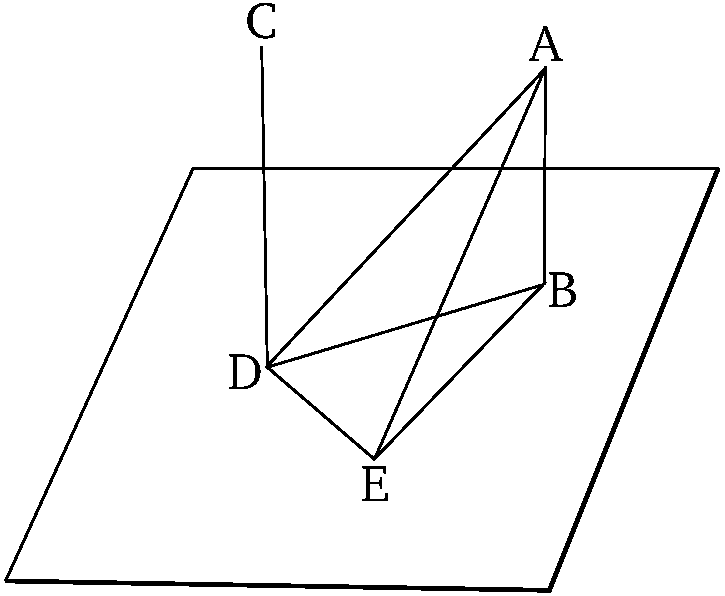
\includegraphics{Book11/fig06e.eps}}

For let the two straight-lines $AB$ and $CD$ be at right-angles
to a reference plane. I say that $AB$ is parallel to $CD$.

For let them meet the reference plane at points $B$ and $D$ (respectively).
And let the straight-line $BD$ be joined. And let $DE$ 
be drawn at right-angles to $BD$ in the reference plane. And
let $DE$ be made equal to $AB$. And let $BE$, $AE$, and $AD$ be joined.

And since $AB$ is at right-angles to the reference plane, it will [thus] also
make right-angles with all straight-lines joined to it which are in the
reference plane [Def.~11.3]. And
$BD$ and $BE$, which are in the reference plane, are each  joined to $AB$.
Thus, each of the angles $ABD$ and $ABE$ are right-angles. So, for the
same (reasons), each of the angles $CDB$ and $CDE$ are also right-angles.
And since $AB$ is equal to $DE$, and $BD$ (is) common, the two
(straight-lines) $AB$ and $BD$ are equal to the two (straight-lines) 
$ED$ and $DB$ (respectively). And they contain right-angles. Thus, the
base $AD$ is equal to the base $BE$ [Prop.~1.4].
And since $AB$ is equal to $DE$, and $AD$ (is) also (equal) to $BE$,  the two
(straight-lines) $AB$ and $BE$ are thus equal to the two (straight-lines) $ED$ and $DA$ (respectively). And their base $AE$ (is) common. Thus, angle $ABE$ is equal to angle $EDA$ [Prop.~1.8]. 
And $ABE$ (is) a right-angle. Thus, $EDA$ (is) also a right-angle.
$ED$ is thus at right-angles to $DA$.  And it is also at right-angles to
each of $BD$ and $DC$. Thus, $ED$ is standing at right-angles
to the three straight-lines $BD$, $DA$, and $DC$ at the (common)
point of section. Thus, the three straight-lines $BD$, $DA$,
and $DC$ are in one plane [Prop.~11.5]. And in
which(ever) plane $DB$ and $DA$ (are found), in that (plane) $AB$ (will) also (be found).
For every triangle is in one plane [Prop.~11.2].
And each of the angles $ABD$ and $BDC$ is a right-angle. Thus, $AB$ is
parallel to $CD$ [Prop.~1.28].

Thus, if  two straight-lines are at right-angles to the same
plane then the straight-lines will be parallel. (Which is) the very thing it
was required to show.}
\end{Parallel}
{\footnotesize\noindent$^\dag$ In other words,
the two straight-lines lie in the same plane, and never meet when
produced in either direction.}

%%%%
%11.7
%%%%
\pdfbookmark[1]{Proposition 11.7}{pdf11.7}
\begin{Parallel}{}{}
\ParallelLText{
\begin{center}
{\large\ggn{7}.}
\end{center}\vspace*{-7pt}

\gr{Ἐὰν >ῶσι δύο εὐθεῖαι παράλληλοι, ληφθῆ| δὲ ἐφ> ἑκατέραξ α\kern -.7pt  ὐτῶν τυθόντα σημεῖα, ἡ ἐπὶ τὰ σημεῖα ἐπιζευγνυμένη εὐθεῖα ἐν τῶ|
α\kern -.7pt  ὐτῶ| ἐπιπέδῳ ἐστὶ ταῖξ παραλλήλοιξ.}

\epsfysize=1.5in
\centerline{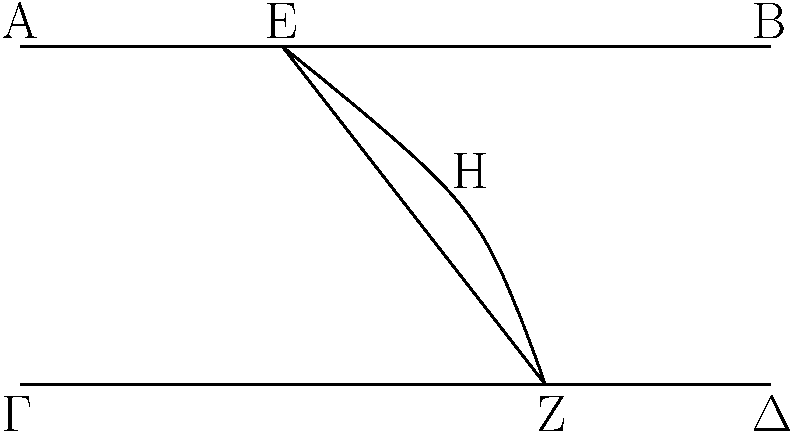
\includegraphics{Book11/fig07g.eps}}

\gr{>'Εστωσαν δύο εὐθεῖαι παράλληλοι αἱ ΑΒ, ΓΔ, καὶ εἰλήφθω ἐφ>
ἑκατέραξ α\kern -.7pt  ὐτῶν τυνθόντα σημεῖα τὰ Ε, Ζ; λέγω, <ότι ἡ ἐπὶ
τὰ Ε, Ζ σημεῖα ἐπιζευγνυμένη εὐθεῖα ἐν τῶ| α\kern -.7pt  ὐτῶ| ἐπιπέδῳ
ἐστὶ ταῖξ παραλλήλοιξ.}

\gr{μ\kern -.7pt  ὴ γάρ, ἀλλ> εἰ δυνατόν, >έστω ἐν μετεωροτέρῳ ὡξ ἡ ΕΗΖ, καὶ
διήθθω διὰ τῆξ ΕΗΖ ἐπίπεδον; τομ\kern -.7pt  ὴν δὴ ποιήσει ἐν τῶ| ὑποκειμένῳ ἐπιπέδῳ εὐθεῖαν. ποιείτω ὡξ τὴν ΕΖ; δύο >άρα
εὐθεῖαι αἱ ΕΗΖ, ΕΖ θωρίον περιέχουσιν; <όπερ ἐστὶν ἀδύνατον.
οὐκ >άρα ἡ ἀπὸ τοῦ Ε ἐπὶ τὸ Ζ ἐπιζευγνυμένη εὐθεῖαι ἐν
μετεωροτέρῳ ἐστὶν ἐπιπέδῳ; ἐν τῶ| διὰ τῶν ΑΒ, ΓΒ >άρα
παραλλήλων ἐστὶν ἐπιπέδῳ ἡ ἀπὸ τοῦ Ε ἐπὶ τὸ Ζ ἐπιζευγνυμένη
εὐθεῖα.}

\gr{Ἐὰν >άρα >ῶσι δύο εὐθεῖαι παράλληλοι, ληφθῆ| δὲ ἐφ> ἑκατέραξ
α\kern -.7pt  ὐτῶν τυθόντα σημεῖα, ἡ ἐπὶ τὰ σημεῖα ἐπιζευγνυμένη
εὐθεῖα ἐν τῶ| α\kern -.7pt  ὐτῶ| ἐπιπέδῳ ἐστὶ ταῖξ παραλλήλοιξ; <όπερ
>έδει δεῖχαι.}}

\ParallelRText{
\begin{center}
{\large Proposition 7}
\end{center}

If there are two parallel straight-lines, and
random points are taken on each of them, then the straight-line joining the
two points is in the same plane as the parallel (straight-lines).

\epsfysize=1.5in
\centerline{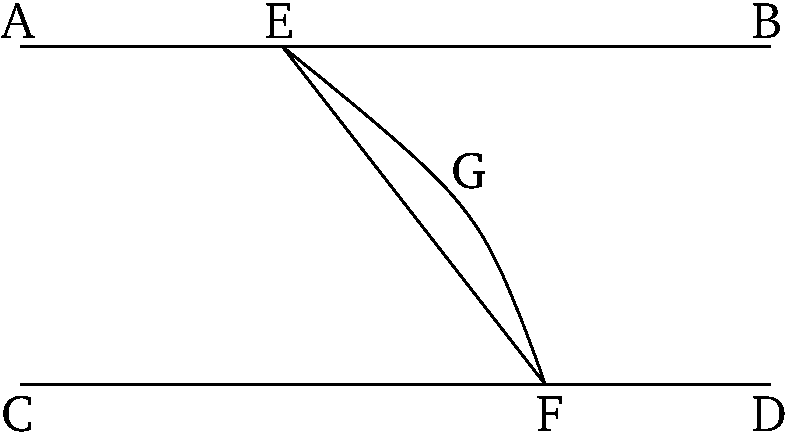
\includegraphics{Book11/fig07e.eps}}

Let $AB$ and $CD$ be two parallel straight-lines, and let the random
points $E$ and $F$ be taken on each of them (respectively). I say that the straight-line joining points $E$ and $F$ is in the same (reference) plane as the parallel
(straight-lines).

For (if)  not, and if possible, let it be in a more elevated (plane), such as
$EGF$. And let a plane be drawn through $EGF$. So it will
make a straight cutting in the reference plane [Prop.~11.3]. Let it make $EF$. Thus, two straight-lines (with the
same end-points), $EGF$ and $EF$,  will enclose an area. The very thing is
impossible. Thus, the straight-line joining $E$ to $F$ is not in a more
elevated plane. The straight-line joining $E$ to $F$ is thus in the plane
through the parallel (straight-lines) $AB$ and $CD$.

Thus, if there are two parallel straight-lines, and
random points are taken on each of them, then the straight-line joining the
two points is in the same plane as the parallel (straight-lines). (Which is)
the very thing it was required to show.}
\end{Parallel}

%%%%
%11.8
%%%%
\pdfbookmark[1]{Proposition 11.8}{pdf11.8}
\begin{Parallel}{}{}
\ParallelLText{
\begin{center}
{\large \ggn{8}.}
\end{center}\vspace*{-7pt}

\gr{Ἐὰν >ῶσι δύο εὐθεῖαι παράλληλοι, ἡ δὲ ἑτέρα α\kern -.7pt  ὐτῶν ἐπιπέδῳ
τινὶ πρὸξ ὀρθὰξ >ῆ|, καὶ ἡ λοιπὴ τῶ| α\kern -.7pt  ὐτῶ| ἐπιπέδῳ πρὸξ ὀρθὰξ
>έσται.}

\gr{>'Εστωσαν δύο εὐθεῖαι παράλληλοι αἱ ΑΒ, ΓΔ, ἡ δὲ ἑτέρα α\kern -.7pt  ὐτῶν
ἡ ΑΒ τῶ| ὑποκειμένῳ ἐπιπέδῳ πρὸξ ὀρθὰξ >έστω; λέγω, <ότι
καὶ ἡ λοιπὴ ἡ ΓΔ τῶ| α\kern -.7pt  ὐτῶ| ἐπιπέδῳ πρὸξ ὀρθὰξ >έσται.}

\gr{Συμβαλλέτωσαν γὰρ αἱ ΑΒ, ΓΔ τῶ| ὑποκειμένῳ ἐπιπέδῳ κατὰ τὰ
Β, Δ σημεῖα, καὶ ἐπεζέυθθω ἡ ΒΔ; αἱ ΑΒ, ΓΔ, ΒΔ >άρα ἐν ἑνί
εἰσιν ἐπιπέδῳ. >ήθθω τῆ| ΒΑ πρὸξ ὀρθὰξ ἐν τῶ| ὑποκειμένῳ
ἐπιπέδῳ ἡ ΔΕ, καὶ κείσθω τῆ| ΑΒ >ίση ἡ ΔΕ, καὶ ἐπεζεύθθωσαν αἱ
ΒΕ, ΑΕ, ΑΔ.}\\

\epsfysize=2.5in
\centerline{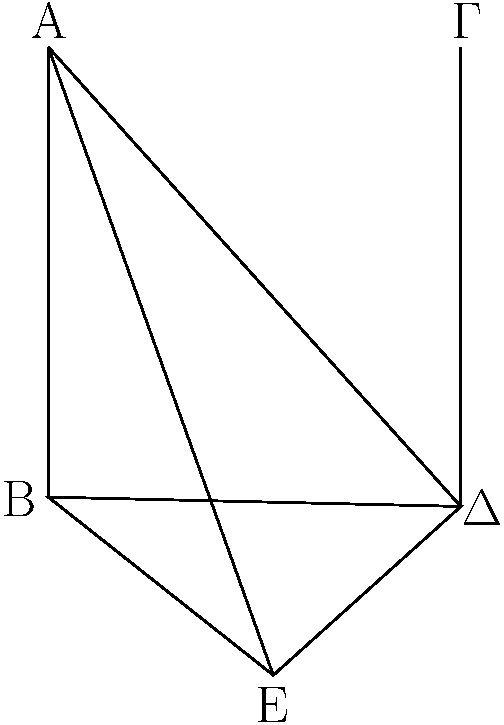
\includegraphics{Book11/fig08g.eps}}

\gr{Καὶ ἐπεὶ ἡ ΑΒ ὁρθή ἐστι πρὸξ τὸ ὑποκείμενον
ἐπίπεδον, καὶ πρὸξ πάσαξ >άρα τὰξ ἁπτομέναξ α\kern -.7pt  ὐτῆξ εὐθείαξ
καὶ ο>ύσαξ ἐν τῶ| ὑποκειμένῳ ἐπιπέδῳ πρὸξ ὀρθάξ
ἐστιν ἡ ΑΒ; ὀρθὴ >άρα [ἐστὶν] ἑκατέρα τῶν ὑπὸ ΑΒΔ, ΑΒΕ
γωνιῶν. καὶ ἐπεὶ εἰξ παραλλήλουξ τὰξ ΑΒ, ΓΔ εὐθεῖα ἐμπέπτωκεν
ἡ ΒΔ, αἱ >άρα ὑπὸ ΑΒΔ, ΓΔΒ γωνίαι δυσὶν ὀρθαῖξ
>ίσαι εἰσίν. ὀρθὴ δὲ ἡ ὑπὸ ΑΒΔ; ὀρθὴ >άρα καὶ ἡ ὑπὸ
ΓΔΒ; ἡ ΓΔ >άρα πρὸξ τὴν ΒΔ ὀρθή ἐστιν. καὶ ἐπεὶ >ίση
ἐστὶν ἡ ΑΒ τῆ| ΔΕ, κοινὴ δὲ ἡ ΒΔ, δύο δὴ αἱ ΑΒ, ΒΔ δυσὶ ταῖξ
ΕΔ, ΔΒ >ίσαι εἰσίν; καὶ γωνία ἡ ὑπὸ ΑΒΔ γωνίᾳ τῆ| ὑπὸ ΕΔΒ >ίση;
ὀρθὴ γὰρ ἑκατέρα; βάσιξ >άρα ἡ ΑΔ βάσει τῆ| ΒΕ >ίση. καὶ
ἐπεὶ >ίση ἐστὶν ἡ μὲν ΑΒ τῆ| ΔΕ, ἡ δὲ ΒΕ τῆ| ΑΔ, δύο δὴ
αἱ ΑΒ, ΒΕ δυσὶ ταῖξ ΕΔ, ΔΑ >ίσαι εἰσὶν ἑκατέρα ἑκατέρᾳ. καὶ
βάσιξ α\kern -.7pt  ὐτῶν κοινὴ ἡ ΑΕ; γωνία >άρα ἡ ὑπὸ ΑΒΕ γωνίᾳ τῆ|
ὑπὸ ΕΔΑ ἐστιν >ίση. ὀρθὴ δὲ ἡ ὑπὸ ΑΒΕ; ὀρθὴ >άρα
καὶ ἡ ὑπὸ ΕΔΑ; ἡ ΕΔ >άρα πρὸξ τὴν ΑΔ ὀρθή ἐστιν.
>έστι δὲ καὶ πρὸξ τὴν ΔΒ ὀρθή; ἡ ΕΔ >άρα καὶ τὼ| διὰ
τῶν ΒΔ, ΔΑ ἐπιπέδῳ ὀρθή
 ἐστιν. καὶ πρὸξ πάσαξ >άρα τὰξ ἁπτομέναξ
α\kern -.5pt  ὐτῆξ εὐθείαξ καὶ ο>ύσαξ ἐν τῶ| διὰ τῶν ΒΔΑ ἐπιπέδῳ
ὀρθὰξ ποιήσει γωνίαξ ἡ ΕΔ. ἐν δὲ τῶ| διὰ τῶν ΒΔΑ ἐπιπέδῳ
ἐστὶν ἡ ΔΓ, ἐπειδήπερ ἐν τῶ| διὰ τῶν ΒΔΑ ἐπιπέδῳ
ἐστὶν αἱ ΑΒ, ΒΔ, ἐν <ῶ| δὲ αἱ ΑΒ, ΒΔ, ἐν τούτῳ ἐστὶ
καὶ ἡ ΔΓ. ἡ ΕΔ >άρα τῆ| ΔΓ πρὸξ ὀρθάξ ἐστιν; <ώστε καὶ ἡ ΓΔ
τῆ| ΔΕ πρὸξ ὀρθάξ ἐστιν. >έστι δὲ καὶ ἡ ΓΔ τῆ| ΒΔ
πρὸξ ὀρθάξ. ἡ ΓΔ >άρα δύο εὐθείαιξ τεμνούσαιξ ἀλλήλαξ
ταῖξ ΔΕ, ΔΒ ἀπὸ τῆξ κατὰ τὸ Δ τομ\kern -.3pt  ῆξ πρὸξ ὀρθὰξ ἐφέστηκεν;
<ώστε ἡ ΓΔ καὶ τῶ| διὰ τῶν ΔΕ, ΔΒ
ἐπιπέδῳ πρὸξ ὀρθάξ ἐστιν. τὸ δὲ διὰ τῶν ΔΕ, ΔΒ ἐπίπεδον
τὸ ὑποκείμενόν ἐστιν; ἡ ΓΔ >άρα τῶ| ὑποκειμένῳ ἐπιπέδῳ
πρὸξ ὀρθάξ ἐστιν.}

\gr{Ἐὰν >άρα >ῶσι δύο εὐθεῖαι παράλληλοι, ἡ δὲ μία α\kern -.7pt  ὐτῶν ἐπιπέδῳ
τινὶ πρὸξ ὀρθὰξ >ῆ|, καὶ ἡ λοιπὴ τῶ|
α\kern -.7pt  ὐτῶ| ἐπιπέδῳ πρὸξ ὀρθὰξ >έσται; <όπερ
>έδει δεῖχαι.}}

\ParallelRText{
\begin{center}
{\large Proposition 8}
\end{center}

If two  straight-lines are parallel, and one of them is at right-angles to some plane, then the remaining (one) will also
be at right-angles to the same plane.

Let $AB$ and $CD$ be two parallel straight-lines, and let one of them, $AB$,
be at right-angles to a reference plane. I say that the remaining (one), $CD$,
will also be at right-angles to the same plane.

For let $AB$ and $CD$ meet the reference plane at points $B$ and $D$
(respectively). And let $BD$ be joined. $AB$, $CD$, and $BD$
are thus in one plane [Prop.~11.7]. 
Let $DE$ be drawn at right-angles to $BD$ in the reference plane, and
let $DE$ be made equal to $AB$, and let $BE$, $AE$, and $AD$ be
joined.

\epsfysize=2.5in
\centerline{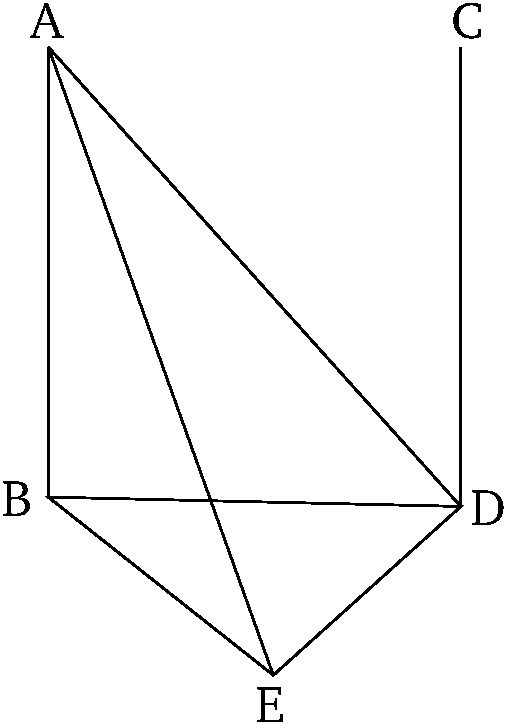
\includegraphics{Book11/fig08e.eps}}

And since $AB$ is at right-angles to the reference plane, $AB$ is thus also
at right-angles to all of the straight-lines joined to it which are in the
reference plane [Def.~11.3].  Thus, the angles $ABD$ and $ABE$ [are] each right-angles. And since the straight-line $BD$ has
met the parallel (straight-lines) $AB$ and $CD$, the (sum of the) angles
$ABD$ and $CDB$ is thus equal to two right-angles [Prop.~1.29]. And $ABD$ (is) a right-angle. Thus, $CDB$ (is)
also a right-angle. $CD$ is thus at right-angles to $BD$. And since $AB$
is equal to $DE$, and $BD$ (is) common, the two (straight-lines) $AB$ and
$BD$ are equal to the two (straight-lines) $ED$ and $DB$ (respectively). And angle
$ABD$ (is) equal to angle $EDB$. For each (is) a right-angle.
Thus, the base $AD$ (is) equal to the base $BE$ [Prop.~1.4]. And since $AB$ is equal to $DE$, and $BE$ to $AD$, 
the two (sides) $AB$, $BE$ are equal to the two (sides) $ED$, $DA$,
respectively. And their base $AE$ is common. Thus, angle $ABE$ is equal to
angle $EDA$ [Prop.~1.8]. And $ABE$ (is) a
right-angle. $EDA$ (is) thus also a right-angle. Thus, $ED$ is
at right-angles to $AD$. And it is also at right-angles to $DB$. Thus, $ED$
is also at right-angles to the plane through $BD$ and $DA$ [Prop.~11.4]. And $ED$ will thus  make right-angles
with all of the straight-lines joined to it which are also in the plane through
$BDA$. And $DC$ is in the plane through $BDA$, inasmuch as
$AB$ and $BD$ are in the plane through $BDA$ [Prop.~11.2], and in which(ever plane)
$AB$ and $BD$ (are found), $DC$ is also (found). Thus, $ED$ is at right-angles to $DC$. Hence, $CD$ is also at right-angles to $DE$. And
$CD$ is also at right-angles to $BD$. Thus, $CD$ is standing  at right-angles
to two straight-lines, $DE$ and $DB$, which meet one another, at the 
(point) of section, $D$. Hence, $CD$ is also at
right-angles to the plane through $DE$ and $DB$ [Prop.~11.4]. And the plane through $DE$ and $DB$ is the reference
(plane). $CD$ is thus at right-angles to the reference plane.

Thus, if  two  straight-lines are parallel, and one of them is at right-angles to some plane, then the remaining (one) will also
be at right-angles to the same plane. (Which is) the very thing it was required to show.}
\end{Parallel}

%%%%
%11.9
%%%%
\pdfbookmark[1]{Proposition 11.9}{pdf11.9}
\begin{Parallel}{}{}
\ParallelLText{
\begin{center}
{\large \ggn{9}.}
\end{center}\vspace*{-7pt}

\gr{Αἱ τῆ| α\kern -.7pt  ὐτῆ| εὐθείᾳ παράλληλοι καὶ μ\kern -.7pt  ὴ ο>ῦσαι α\kern -.5pt  ὐτῆ| ἐν
τῶ| α\kern -.3pt  ὐτῶ| ἐπιπέδῳ καὶ ἀλλήλαιξ εἰσὶ παράλληλοι.}\\

\epsfysize=1.6in
\centerline{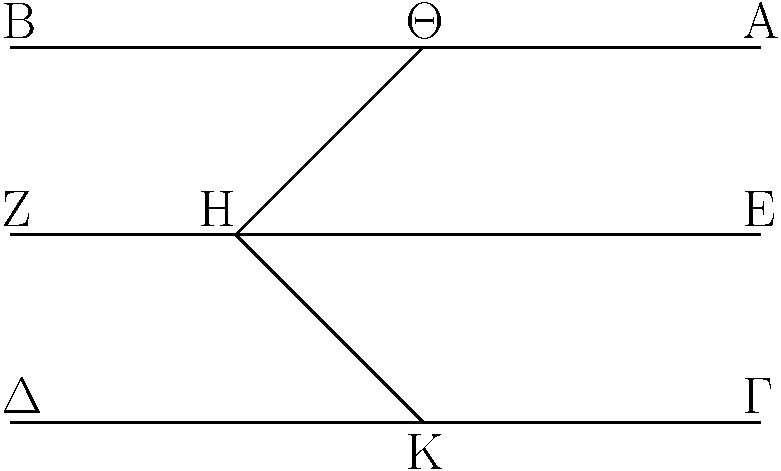
\includegraphics{Book11/fig09g.eps}}

\gr{>'Εστω γὰρ ἑκατέρα τῶν ΑΒ, ΓΔ τῆ| ΕΖ παράλληλοξ μ\kern -.7pt  ὴ ο>ῦσαι
α\kern -.7pt  ὐτῆ| ἐν τῶ| α\kern -.5pt  ὐτῶ| ἐπιπέδῳ; λέγω, <ότι παράλληλόξ ἐστιν
ἡ ΑΒ τῆ| ΓΔ.}

\gr{Εἰλήφθω γὰρ ἐπὶ τῆξ ΕΖ τυθὸν σημεῖον τὸ Η, καὶ ἀπ>
α\kern -.7pt  ὐτοῦ τῆ| ΕΖ ἐν μὲν τῶ| διὰ τῶν ΕΖ, ΑΒ ἐπιπέδῳ πρὸξ
ὀρθὰξ >ήθθω ἡ ΗJ, ἐν δὲ τῶ| διὰ τῶν ΖΕ, ΓΔ τῆ| ΕΖ πάλιν
πρὸξ ὀρθὰξ >ήθθω ἡ ΗΚ.}

\gr{Καὶ ἐπεὶ ἡ ΕΖ πρὸξ ἑκατέραν
τῶν ΗJ, ΗΚ ὀρθή ἐστιν, ἡ ΕΖ
>άρα καὶ
τῶ| διὰ τῶν ΗJ, ΗΚ ἐπιπέδῳ πρὸξ ὀρθάξ ἐστιν. καί ἐστιν
ἡ ΕΖ τῆ| ΑΒ παράλληλοξ; καὶ ἡ ΑΒ >άρα τῶ| διὰ τῶν JΗΚ ἐπιπέδῳ
πρὸξ ὀρθάξ ἐστιν. διὰ τὰ α\kern -.7pt  ὐτὰ δὴ καὶ ἡ ΓΔ τῶ| διὰ τῶν
JΗΚ ἐπιπέδῳ πρὸξ ὀρθάξ ἐστιν; ἑκατέρα >άρα τῶν ΑΒ, ΓΔ τῶ|
διὰ τῶν JΗΚ ἐπιπέδῳ πρὸξ ὀρθάξ ἐστιν. ἒαν δὲ δύο εὐθεῖαι
τῶ| α\kern -.7pt  ὐτῶ| ἐπιπέδῳ πρὸξ ὀρθὰξ >ῶσιν, παράλληλοί εἰσιν
αἱ εὐθεῖαι; παράλληλοξ >άρα ἐστὶν ἡ ΑΒ τῆ| ΓΔ; <όπερ
>έδει δεῖχαι.}}

\ParallelRText{
\begin{center}
{\large Proposition 9}
\end{center}

(Straight-lines) parallel to the same straight-line,
and which are not in the same plane as it, are also parallel to one another.

\epsfysize=1.6in
\centerline{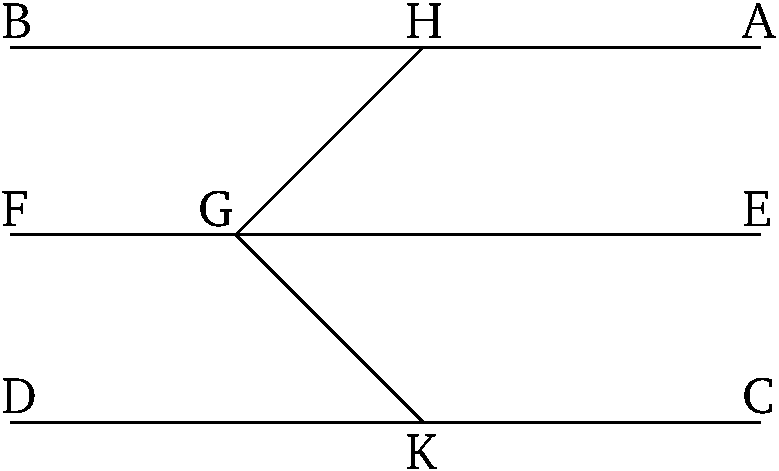
\includegraphics{Book11/fig09e.eps}}

For let $AB$ and $CD$ each be parallel to $EF$, not being in the
same plane as it. I say that $AB$ is parallel to $CD$.

For let some point $G$ be taken at random on $EF$. And from it
let $GH$ be drawn at right-angles to $EF$ in the plane through
$EF$ and $AB$. And let $GK$ be drawn, again at right-angles
to $EF$, in the plane through  $FE$ and $CD$.

And since $EF$ is at right-angles to each of $GH$ and $GK$, $EF$
is thus also at right-angles to the plane through $GH$ and $GK$ 
[Prop.~11.4]. And $EF$ is parallel to
$AB$. Thus, $AB$ is also at right-angles to the plane through $HGK$
[Prop.~11.8]. So, for the same (reasons), $CD$
is also at right-angles to the plane through $HGK$.  Thus, $AB$ and
$CD$ are each at right-angles to the plane through $HGK$.
And if two straight-lines are at right--angles to the same plane then the 
straight-lines are parallel [Prop.~11.6]. Thus, $AB$ is parallel to
$CD$. (Which is) the very thing it was required to show.}
\end{Parallel}

%%%%
%11.10
%%%%
\pdfbookmark[1]{Proposition 11.10}{pdf11.10}
\begin{Parallel}{}{}
\ParallelLText{
\begin{center}
{\large \ggn{10}.}
\end{center}\vspace*{-7pt}

\gr{Ἐὰν δύο εὐθεῖαι ἁπτόμεναι ἀλλήλων παρὰ δύο εὐθείαξ ἁπτομέναξ
ἀλλήλων >ῶσι μ\kern -.7pt  ὴ ἐν τῶ| α\kern -.7pt  ὐτῶ| ἐπιπέδῳ, <ίσαξ γωνίαξ
περιέχουσιν.}

\gr{Δύο γὰρ εὐθεῖαι αἱ ΑΒ, ΒΓ ἁπτόμεναι ἀλλήλων παρὰ δύο
εὐθείαξ τὰξ ΔΕ, ΕΖ ἁπτομέναξ ἀλλήλων >έστωσαν μ\kern -.7pt  ὴ ἐν
τῶ| α\kern -.7pt  ὐτῶ| ἐπιπέδῳ; λέγω, <ότι >ίση ἐστὶν ἡ ὑπὸ
ΑΒΓ γωνία τῆ| ὑπὸ ΔΕΖ.}

\gr{Ἀπειλήφθωσαν γὰρ αἱ ΒΑ, ΒΓ, ΕΔ, ΕΖ >ίσαι ἀλλήλαιξ, καὶ
ἐπεζεύθθωσαν αἱ ΑΔ, ΓΖ, ΒΕ, ΑΓ, ΔΖ.}

\gr{Καὶ ἐπεὶ ἡ ΒΑ
τῆ| ΕΔ >ίση ἐστὶ καὶ παράλληλοξ, καὶ ἡ ΑΔ >άρα τῆ| ΒΕ >ίση
ἐστὶ καὶ παράλληλοξ.
 διὰ τὰ α\kern -.7pt  ὐτὰ δὴ καὶ ἡ ΓΖ τῆ| ΒΕ >ίση ἐστὶ καὶ παράλληλοξ; ἑκατέρα
 >άρα τῶν ΑΔ, ΓΖ τῆ| ΒΕ >ίση ἐστὶ καὶ παράλληλοξ. αἱ δὲ τῆ|
 α\kern -.7pt  ὐτῆ| εὐθείᾳ παράλληλοι καὶ μ\kern -.5pt  ὴ ο>ῦσαι α\kern -.3pt  ὐτῆ| ἐν τῶ| α\kern -.7pt  ὐτῶ|
  ἐπιπέδῳ καὶ ἀλλήλαιξ εἰσὶ παράλληλοι; παράλληλοξ >άρα ἐστὶν
 ἡ ΑΔ τῆ| ΓΖ καὶ >ίση. καὶ ἐπιζευγνύουσιν α\kern -.7pt  ὐτὰξ αἱ
 ΑΓ, ΔΖ; καὶ ἡ ΑΓ >άρα τῆ| ΔΖ >ίση ἐστὶ καὶ παράλληλοξ.
 καὶ ἐπεὶ δύο αἱ ΑΒ, ΒΓ δυσὶ ταῖξ ΔΕ, ΕΖ >ίσαι εἰσίν,
 καὶ βάσιξ ἡ ΑΓ βάσει τῆ| ΔΖ >ίση, γωνία >άρα ἡ ὑπὸ
 ΑΒΓ γωνίᾳ τῆ| ὑπὸ ΔΕΖ ἐστιν >ίση.}\\~\\

\epsfysize=2.in
\centerline{
\includegraphics{Book11/fig10g.eps}}
 
 \gr{Ἐὰν >άρα δύο εὐθεῖαι ἁπτόμεναι ἀλλήλων παρὰ δύο εὐθείαξ ἁπτομέναξ
ἀλλήλων >ῶσι μ\kern -.7pt  ὴ ἐν τῶ| α\kern -.7pt  ὐτῶ| ἐπιπέδῳ, <ίσαξ γωνίαξ
περιέχουσιν; <όπερ >έδει δεῖχαι.}}

\ParallelRText{
\begin{center}
{\large Proposition 10}
\end{center}

If two straight-lines joined to one another
are (respectively) parallel to two straight-lines joined to one another, (but are) not in the same
plane, then they will contain equal angles.

For let the two straight-lines joined to one another, $AB$ and $BC$, be (respectively) parallel to the two straight-lines joined to one another, $DE$ and $EF$, (but) not in the same plane. I say that angle $ABC$ is equal to
(angle) $DEF$.

For let $BA$, $BC$, $ED$, and $EF$ be cut off (so as to be, respectively) equal
to one another. And let $AD$, $CF$, $BE$, $AC$, and $DF$
be joined.

And since $BA$ is equal and parallel to $ED$, $AD$ is thus also equal
and parallel to $BE$ [Prop.~1.33]. So, for the
same reasons, $CF$ is also equal and parallel to $BE$. Thus, $AD$ and
$CF$ are each equal and parallel to $BE$. And straight-lines parallel to
the same straight-line, and which are not in the same plane as it, are also parallel
to one another [Prop.~11.9]. Thus, $AD$
is parallel and equal to $CF$. And $AC$ and $DF$ join them. Thus, $AC$
is also equal and parallel to $DF$ [Prop.~1.33].
And since the two (straight-lines) $AB$ and $BC$ are equal to the
two (straight-lines) $DE$ and $EF$ (respectively),  and the base $AC$  (is) equal to the base $DF$, the angle $ABC$ is thus equal to the (angle) $DEF$   
[Prop.~1.8].

\epsfysize=2.in
\centerline{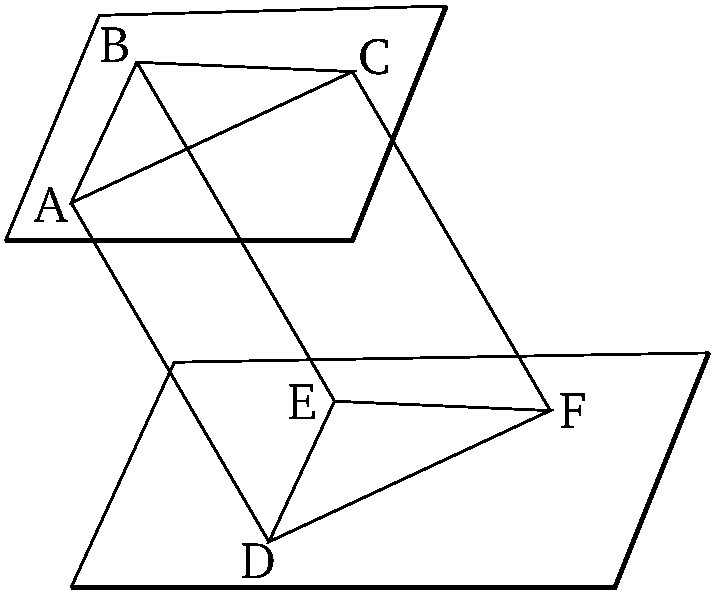
\includegraphics{Book11/fig10e.eps}}

Thus, if two straight-lines joined to one another
are (respectively) parallel to two straight-lines joined to one another, (but are) not in the same
plane, then they will contain equal angles. (Which is) the very thing it
was required to show.}
\end{Parallel}

%%%%
%11.11
%%%%
\pdfbookmark[1]{Proposition 11.11}{pdf11.11}
\begin{Parallel}{}{}
\ParallelLText{
\begin{center}
{\large \ggn{11}.}
\end{center}\vspace*{-7pt}

\gr{Ἀπὸ τοῦ δοθέντοξ σημείου μετεώρου ἐπὶ τὸ δοθὲν ἐπίπεδον
κάθετον εὐθεῖαν γραμμ\kern -.7pt  ὴν ἀγαγεῖν.}

\epsfysize=2.5in
\centerline{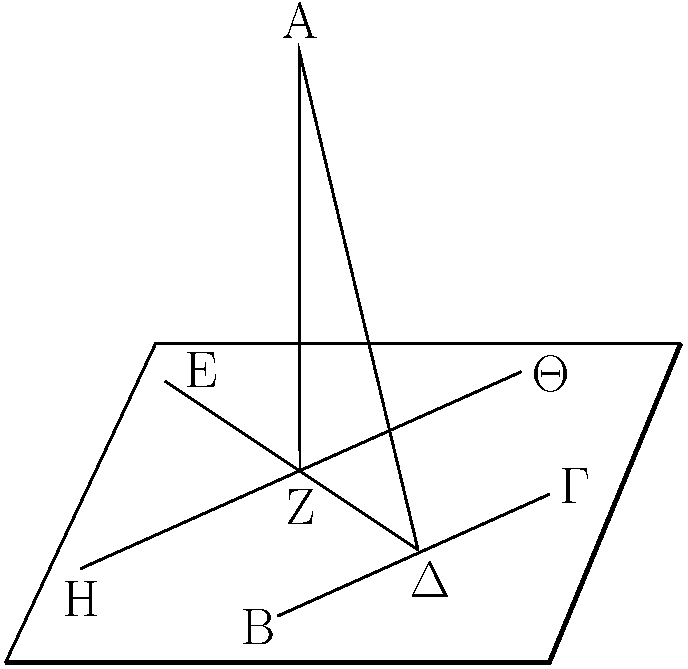
\includegraphics{Book11/fig11g.eps}}

\gr{>'Εστω τὸ μὲν δοθὲν σημεῖον μετέωρον τὸ Α, τὸ δὲ δοθὲν ἐπίπεδον
τὸ ὑποκείμενον; δεῖ δὴ ἀπὸ τοῦ Α σημείου ἐπὶ τὸ ὑποκείμενον
ἐπίπεδον κάθετον εὐθεῖαν γραμμ\kern -.7pt  ὴν ἀγαγεῖν.}

\gr{Διήθθω γάρ τιξ ἐν τῶ| ὑποκειμένῳ ἐπιπέδῳ εὐθεῖα,
ὡξ >έτυθεν, ἡ ΒΓ, καὶ >ήθθω ἀπὸ τοῦ Α σημείου ἐπὶ τὴν ΒΓ
κάθετοξ ἡ ΑΔ. εἰ μὲν ο>ῦν ἡ ΑΔ κάθετόξ ἐστι καὶ ἐπὶ τὸ
ὑποκείμενον ἐπίπεδον, γεγονὸξ >ὰν ε>ίη
τὸ ἐπιταθθέν. εἰ δὲ ο>ύ, >ήθθω ἀπὸ τοῦ Δ σημείου τῆ| ΒΓ
ἐν τῶ| ὑποκειμένῳ ἐπιπέδῳ πρὸξ ὀρθὰξ ἡ ΔΕ, καὶ
>ήθθω ἀπὸ τοῦ Α ἐπὶ τὴν ΔΕ κάθετοξ ἡ ΑΖ, καὶ διὰ τοῦ Ζ
σημείου τῆ| ΒΓ παράλληλοξ >ήθθω ἡ ΗJ.}

\gr{Καὶ ἐπεὶ ἡ ΒΓ ἑκατέρᾳ τῶν ΔΑ, ΔΕ πρὸξ ὀρθάξ ἐστιν,
ἡ ΒΓ >άρα καὶ τῶ| διὰ τῶν ΕΔΑ ἐπιπέδῳ πρὸξ ὀρθάξ
ἐστιν. καί ἐστιν α\kern -.7pt  ὐτῆ| παράλληλοξ ἡ ΗJ; ἒαν δὲ >ῶσι
δύο εὐθεῖαι παράλληλοι, ἡ δὲ μία α\kern -.7pt  ὐτῶν ἐπιπέδῳ
τινὶ πρὸξ ὀρθὰξ >ῆ|, καὶ ἡ λοιπὴ τῶ| α\kern -.5pt  ὐτῶ| ἐπιπέδῳ
πρὸξ ὀρθὰξ >έσται; καὶ ἡ ΗJ >άρα τῶ| διὰ τῶν ΕΔ, ΔΑ ἐπιπέδῳ
πρὸξ ὀρθάξ ἐστιν. καὶ πρὸξ πάσαξ >άρα τὰξ ἁπτομέναξ α\kern -.3pt  ὐτῆξ
εὐθείαξ καὶ ο>ύσαξ ἐν τῶ| διὰ τῶν ΕΔ, ΔΑ ἐπιπέδῳ ὀρθή
ἐστιν ἡ ΗJ. <άπτεται δὲ α\kern -.7pt  ὐτῆξ ἡ ΑΖ ο>ῦσα ἐν τῶ| διὰ
τῶν ΕΔ, ΔΑ ἐπιπέδῳ; ἡ ΗJ >άρα ὀρθή ἐστι πρὸξ
τὴν ΖΑ; <ώστε καὶ ἡ ΖΑ ὀρθή ἐστι πρὸξ τὴν JΗ. >έστι
δὲ ἡ ΑΖ καὶ πρὸξ τὴν ΔΕ ὀρθή; ἡ ΑΖ >άρα πρὸξ ἑκατέραν
τῶν ΗJ, ΔΕ ὀρθή ἐστιν. ἒαν δὲ εὐθεῖα δυσὶν εὐθείαιξ τεμνούσαιξ
ἀλλήλαξ ἐπὶ τῆξ τομ\kern -.7pt  ῆξ πρὸξ ὀρθὰξ 
ἐπισταθῆ|, καὶ τῶ| δι> α\kern -.7pt  ὐτῶν ἐπιπέδῳ πρὸξ ὀρθὰξ
>έσται; ἡ ΖΑ >άρα τῶ|
διὰ τῶν ΕΔ, ΗJ ἐπιπέδῳ πρὸξ ὀρθάξ ἐστιν. τὸ δὲ διὰ τῶν
ΕΔ, ΗJ ἐπίπεδόν ἐστι τὸ ὑποκείμενον; ἡ ΑΖ >άρα τῶ|
ὑποκειμένῳ ἐπιπέδῳ πρὸξ ὀρθάξ ἐστιν.}

\gr{Ἀπὸ τοῦ >άρα δοθέντοξ σημείου μετεώρου τοῦ Α ἐπὶ τὸ ὑποκείμενον ἐπίπεδον κάθετοξ εὐθεῖα γραμμ\kern -.7pt  ὴ >ῆκται ἡ ΑΖ;
 <όπερ >έδει ποιῆσαι.}}
 
\ParallelRText{
\begin{center}
{\large Proposition 11}
\end{center}

To draw a perpendicular straight-line from a
given raised point to a given plane.

\epsfysize=2.5in
\centerline{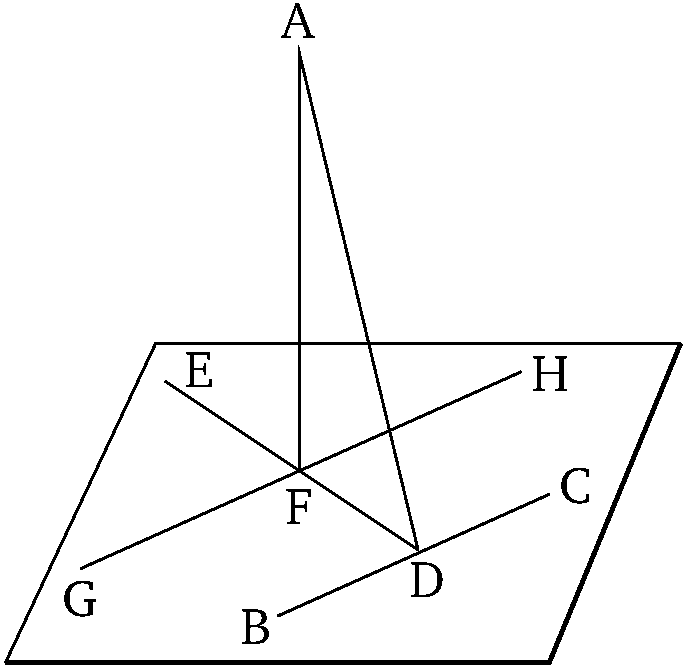
\includegraphics{Book11/fig11e.eps}}

Let $A$ be the given raised point, and the given plane the reference (plane).
So, it is required to draw a perpendicular straight-line from point $A$
to the reference plane.

Let some random straight-line $BC$ be drawn across in the reference plane, and let the  (straight-line) $AD$ be
drawn from point $A$ perpendicular to $BC$ [Prop.~1.12].
If, therefore, $AD$ is also perpendicular to the reference plane then that which
was prescribed will have occurred. And, if not, let $DE$ be
drawn in the reference plane from point $D$  at right-angles to $BC$ [Prop.~1.11], and let the (straight-line) $AF$
be drawn from $A$ perpendicular to $DE$ [Prop.~1.12],
and let $GH$ be drawn through point $F$, parallel to $BC$ [Prop.~1.31].

And since $BC$ is at right-angles to each of $DA$ and $DE$, $BC$ is
thus also at right-angles to the plane through $EDA$ [Prop.~11.4]. And $GH$ is parallel to it. And if two 
straight-lines are parallel, and one of them is at right-angles to some plane, then the
remaining (straight-line) will also be at right-angles to the same plane
[Prop.~11.8]. Thus, $GH$ is also
at right-angles to the plane through $ED$ and $DA$. And $GH$ is thus
at right-angles to all of the straight-lines joined to it which are also
in the plane through $ED$ and $AD$ [Def.~11.3].
And $AF$, which is in the plane through $ED$ and $DA$, is joined to it.
Thus, $GH$ is at right-angles to $FA$. Hence, $FA$ is also
at right-angles to $HG$. And $AF$ is also at right-angles to $DE$.
Thus, $AF$ is at right-angles to each of $GH$ and $DE$. And if a straight-line is set up at right-angles to two straight-lines cutting one another, at the
point of section, then it will also be at right-angles to the plane through them
[Prop.~11.4]. Thus, $FA$ is at right-angles to the
plane through $ED$ and $GH$. And the plane through $ED$ and
$GH$ is the reference (plane). Thus, $AF$ is at right-angles to
the reference plane.

Thus, the  straight-line $AF$ has been drawn from the given raised point 
$A$ perpendicular to the reference plane. (Which is) the very thing it was required to do.}
\end{Parallel}

%%%%
%11.12
%%%%
\pdfbookmark[1]{Proposition 11.12}{pdf11.12}
\begin{Parallel}{}{}
\ParallelLText{
\begin{center}
{\large \ggn{12}.}
\end{center}\vspace*{-7pt}

\gr{Τῶ| δοθέντι ἐπιπέδῳ ἀπὸ τοῦ πρὸξ α\kern -.7pt  ὐτῶ| δοθέντοξ σημείου
πρὸξ ὀρθὰξ εὐθεῖαν γραμμ\kern -.7pt  ὴν ἀναστῆσαι.}

\epsfysize=2.75in
\centerline{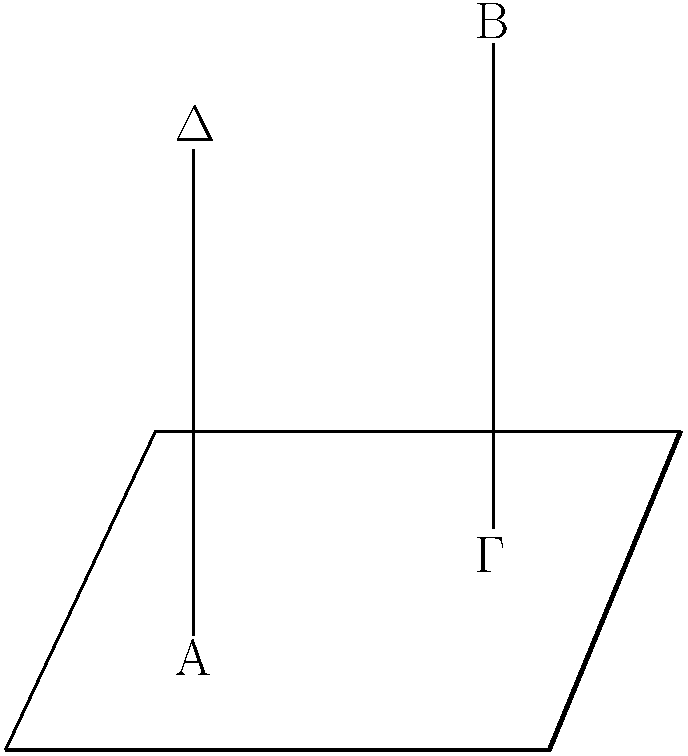
\includegraphics{Book11/fig12g.eps}}

\gr{>'Εστω τὸ μὲν δοθὲν ἐπίπεδον τὸ ὑποκείμενον, τὸ δὲ πρὸξ
α\kern -.7pt  ὐτῶ| σημεῖον τὸ Α; δεῖ δὴ ἀπὸ τοῦ Α σημείου
τῶ| ὑποκειμένῳ ἐπιπέδῳ πρὸξ ὀρθὰξ εὐθεῖαν γραμμ\kern -.7pt  ὴν
ἀναστῆσαι.}

\gr{Νενοήσθω τι σημεῖον μετέωρον τὸ Β, καὶ ἀπὸ τοῦ Β ἐπὶ
τὸ ὑποκείμενον ἐπίπεδον κάθετοξ >ήθθω ἡ ΒΓ, καὶ διὰ
τοῦ Α σημείου τῆ| ΒΓ παράλληλοξ >ήθθω ἡ ΑΔ.}

\gr{Ἐπεὶ ο~ὐν δύο εὐθεῖαι παράλληλοί εἰσιν αἱ ΑΔ, ΓΒ, ἡ δὲ μία
α\kern -.7pt  ὐτῶν ἡ ΒΓ τῶ| ὑποκειμένῳ ἐπιπέδῳ πρὸξ ὀρθάξ
ἐστιν, καὶ ἡ λοιπὴ >άρα ἡ ΑΔ τῶ| ὑποκειμένῳ ἐπιπέδῳ
πρὸξ ὀρθὰξ ἐστιν.}

\gr{Τῶ| >άρα δοθέντι ἐπιπέδῳ ἀπὸ τοῦ πρὸξ α\kern -.7pt  ὐτῶ| σημείου
τοῦ Α πρὸξ ὀρθὰξ ἀνέσταται ἡ ΑΔ; <όπερ >έδει ποιῆσαι.
}}

\ParallelRText{
\begin{center}
{\large Proposition 12}
\end{center}

To set up a straight-line at right-angles to a given plane from a given point in it.

\epsfysize=2.75in
\centerline{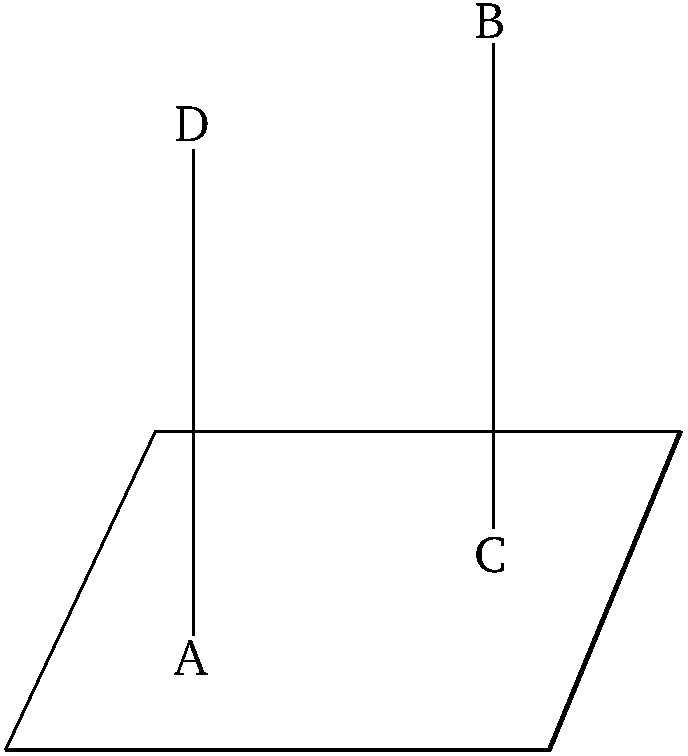
\includegraphics{Book11/fig12e.eps}}

Let the given plane be the reference (plane), and $A$ a point in it. So, it is required to set up a straight-line at right-angles to the reference plane at point $A$.

Let some raised point $B$ be assumed, and let the perpendicular
(straight-line) $BC$ be drawn from $B$ to the reference plane
[Prop.~11.11]. And let $AD$ be drawn
from point $A$ parallel to $BC$ [Prop.~1.31].

Therefore, since $AD$ and $CB$ are two parallel straight-lines, and one of
them, $BC$, is at right-angles to the reference plane, the remaining (one) $AD$
is thus also at right-angles to the reference plane [Prop.~11.8].

Thus, $AD$ has been set up at right-angles to the given plane, from the
 point in it, $A$. (Which is) the very thing it was required to do.}
\end{Parallel}

%%%%
%11.13
%%%%
\pdfbookmark[1]{Proposition 11.13}{pdf11.13}
\begin{Parallel}{}{}
\ParallelLText{
\begin{center}
{\large \ggn{13}.}
\end{center}\vspace*{-7pt}

\gr{Ἀπὸ τοῦ α\kern -.7pt  ὐτοῦ σημείου τῶ| α\kern -.7pt  ὐτῶ| ἐπιπέδῳ δύο εὐθεῖαι
πρὸξ ὀρθὰξ οὐκ ἀναστήσονται ἐπὶ τὰ α\kern -.5pt  ὐτὰ μέρη.}

\epsfysize=2.5in
\centerline{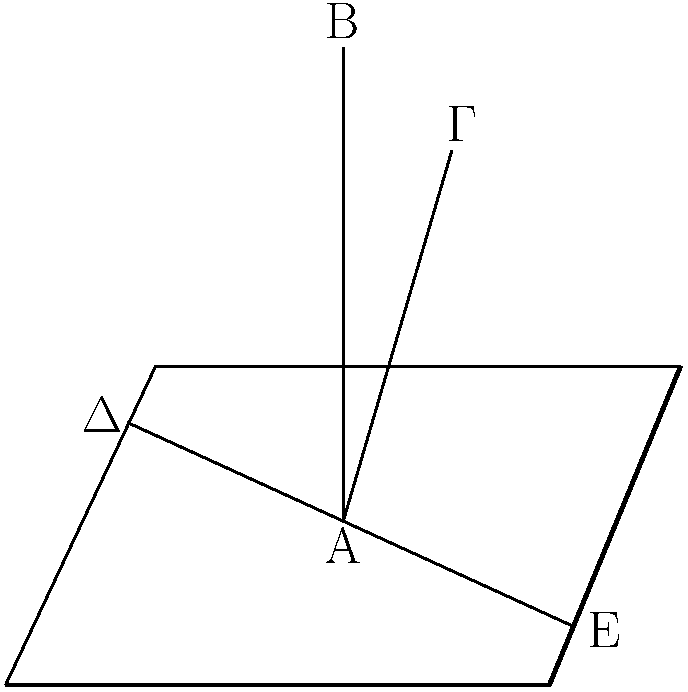
\includegraphics{Book11/fig13g.eps}}

\gr{Εἰ γὰρ δυνατόν, ἀπὸ τοῦ α\kern -.7pt  ὐτοῦ σημείου τοῦ Α τῶ| ὑποκειμένῳ
ἐπιπέδῳ δύο εὐθεῖαι αἱ ΑΒ, ΒΓ πρὸξ ὀρθὰξ ἀνεστάτωσαν ἐπὶ τὰ
α\kern -.7pt  ὐτὰ μέρη, καὶ διήθθω τὸ διὰ τῶν ΒΑ, ΑΓ ἐπὶπεδον; τομ\kern -.5pt  ὴν
δὴ ποιήσει διὰ τοῦ Α ἐν τῶ| ὑποκειμένῳ ἐπιπέδῳ εὐθεῖαν. ποιείτω τὴν ΔΑΕ; αἱ >άρα ΑΒ, ΑΓ, ΔΑΕ εὐθεῖαι ἐν ἑνι εἰσιν
ἐπιπέδῳ. καὶ ἐπεὶ ἡ ΓΑ τῶ| ὑποκειμένῳ ἐπιπέδῳ πρὸξ ὀρθάξ
ἐστιν, καὶ πρὸξ πάσαξ >άρα τὰξ ἁπτομέναξ α\kern -.3pt  ὐτῆξ εὐθείαξ καὶ 
ο>ύσαξ ἐν τῶ| ὑποκειμένῳ ἐπιπέδῳ ὀρθὰξ ποιήσει γωνίαξ.
<άπτεται δὲ α\kern -.7pt  ὐτῆξ ἡ ΔΑΕ ο>ῦσα ἐν τῶ| ὑποκειμένῳ ἐπιπέδῳ;
ἡ >άρα ὑπὸ ΓΑΕ γωνία ὀρθή ἐστιν. διὰ τὰ α\kern -.7pt  ὐτὰ δὴ καὶ ἡ ὑπὸ 
ΒΑΕ ὀρθή ἐστιν; >ίση >άρα ἡ ὑπὸ ΓΑΕ τῆ| ὑπὸ ΒΑΕ  καί εἰσιν ἐν ἑνὶ
ἐπιπέδῳ; <όπερ ἐστὶν ἀδύνατον.}

\gr{Οὐκ >άρα ἀπὸ τοῦ α\kern -.7pt  ὐτοῦ σημείου τῶ| α\kern -.7pt  ὐτῶ| ἐπιπέδῳ δύο εὐθεῖαι
πρὸξ ὀρθὰξ ἀνασταθήσονται ἐπὶ τὰ α\kern -.5pt  ὐτὰ μέρη; <όπερ >έδει δεῖχαι.}}

\ParallelRText{
\begin{center}
{\large Proposition 13}
\end{center}

Two (different) straight-lines cannot be set up at the same point at right-angles to the same plane, on the same side.

\epsfysize=2.5in
\centerline{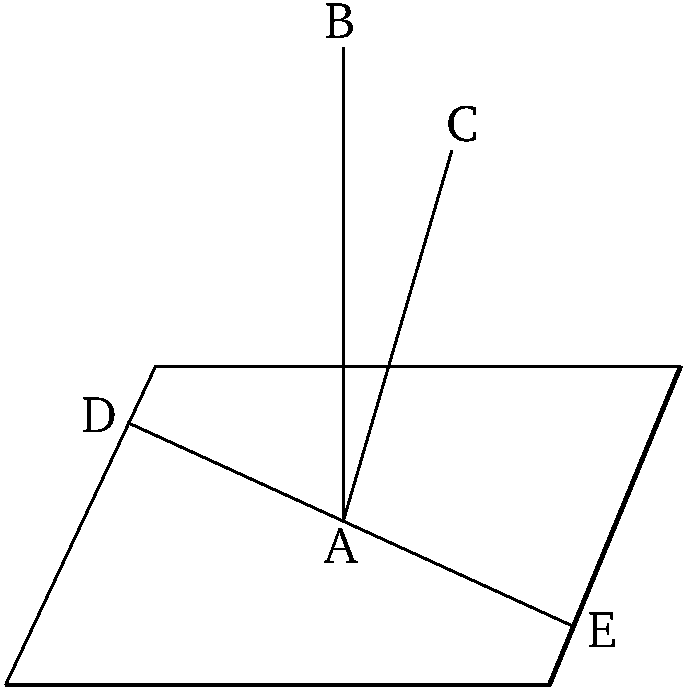
\includegraphics{Book11/fig13e.eps}}

For, if possible, let the two straight-lines $AB$ and $AC$ be
set up at the same point $A$ at right-angles to the reference plane, on the same
side. And let the plane through $BA$ and $AC$ be drawn. So
it will make a straight cutting (passing) through (point) $A$ in the reference plane [Prop.~11.3]. Let it have made $DAE$. Thus, $AB$,
$AC$, and $DAE$ are straight-lines in one plane. And
since $CA$ is at right-angles to the reference plane, it will thus
also make right-angles with all of the straight-lines  joined to it which are
also in the reference plane [Def.~11.3]. 
And $DAE$, which is in the reference plane, is joined to it. Thus, angle
$CAE$ is a right-angle. So, for the same (reasons), $BAE$ is also
a right-angle. Thus, $CAE$ (is) equal to  $BAE$. And they are in one
plane. The very thing is impossible.

Thus, two (different) straight-lines cannot be set up at the same point at right-angles to the same plane, on the same side. (Which is) the very thing it was required to show.\\~\\}
\end{Parallel}

%%%%
%11.14
%%%%
\pdfbookmark[1]{Proposition 11.14}{pdf11.14}
\begin{Parallel}{}{}
\ParallelLText{
\begin{center}
{\large \ggn{14}.}
\end{center}\vspace*{-7pt}

\gr{Πρὸξ <ὰ ἐπίπεδα ἡ α\kern -.7pt  ὐτὴ εὐθεῖα ὀρθή ἐστιν,
παράλληλα >έσται τὰ ἐπίπεδα.}

\gr{Εὐθεῖα γάρ τιξ ἡ ΑΒ πρὸξ ἑκάτερον τῶν ΓΔ, ΕΖ
ἐπιπέδων πρὸξ ὀρθὰξ >έστω; λέγω, <ότι παράλληλά ἐστι τὰ
ἐπίπεδα.}

\epsfysize=2.in
\centerline{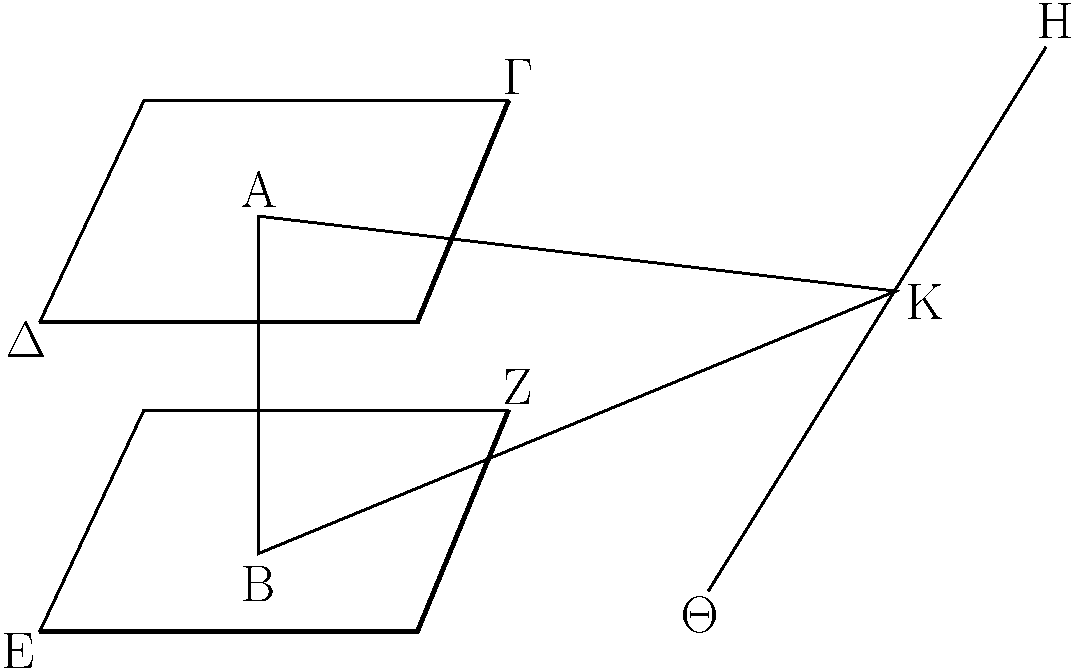
\includegraphics{Book11/fig14g.eps}}

\gr{Εἰ γὰρ μ\kern -.7pt  ή, ἐκβαλλόμενα συμπεσοῦνται. συμπιπτέτ\-ωσαν; ποιήσουσι
δὴ κοινὴν τομ\kern -.7pt  ὴν εὐθεῖαν. ποιείτωσαν τὴν ΗJ, καὶ εἰλήφθω
ἐπὶ τῆξ ΗJ τυθὸν σημεῖον τὸ Κ, καὶ ἐπεζεύθθωσαν αἱ ΑΚ,
ΒΚ.}

\gr{Καὶ ἐπεὶ ἡ ΑΒ ὀρθή ἐστι πρὸξ τὸ ΕΖ ἐπίπεδον,
καὶ πρὸξ τὴν ΒΚ >άρα εὐθεῖαν ο>ῦσαν ἐν τῶ| ΕΖ ἐκβληθέντι
ἐπιπέδῳ ὀρθή ἐστιν ἡ ΑΒ; ἡ >άρα ὑπὸ ΑΒΚ
γωνία ὀρθή ἐστιν. διὰ τὰ α\kern -.7pt  ὐτὰ δὴ καὶ ἡ ὑπὸ
ΒΑΚ ὀρθή ἐστιν. τριγώνου δὴ τοῦ ΑΒΚ αἱ δύο γωνίαι
αἱ ὑπὸ ΑΒΚ, ΒΑΚ δυσὶν ὀρθαῖξ εἰσιν >ίσαι;
<όπερ ἐστὶν ἀδύνατον. οὐκ >άρα τὰ ΓΔ, ΕΖ ἐπίπεδα
ἐκβαλλόμενα συμπεσοῦνται; παράλληλα >άρα ἐστὶ τὰ ΓΔ, ΕΖ
ἐπίπεδα.}

\gr{Πρὸξ <ὰ ἐπίπεδα >άρα ἡ α\kern -.7pt  ὐτὴ εὐθεῖα ὀρθή ἐστιν,
παράλληλά ἐστι τὰ ἐπίπεδα; <όπερ >έδει δεῖχαι.}}

\ParallelRText{
\begin{center}
{\large Proposition 14}
\end{center}

Planes to which the same straight-line
is at right-angles will be  parallel planes.

For let some straight-line $AB$ be at right-angles to each of the planes
$CD$ and $EF$. I say that the planes are parallel.\\

\epsfysize=2.in
\centerline{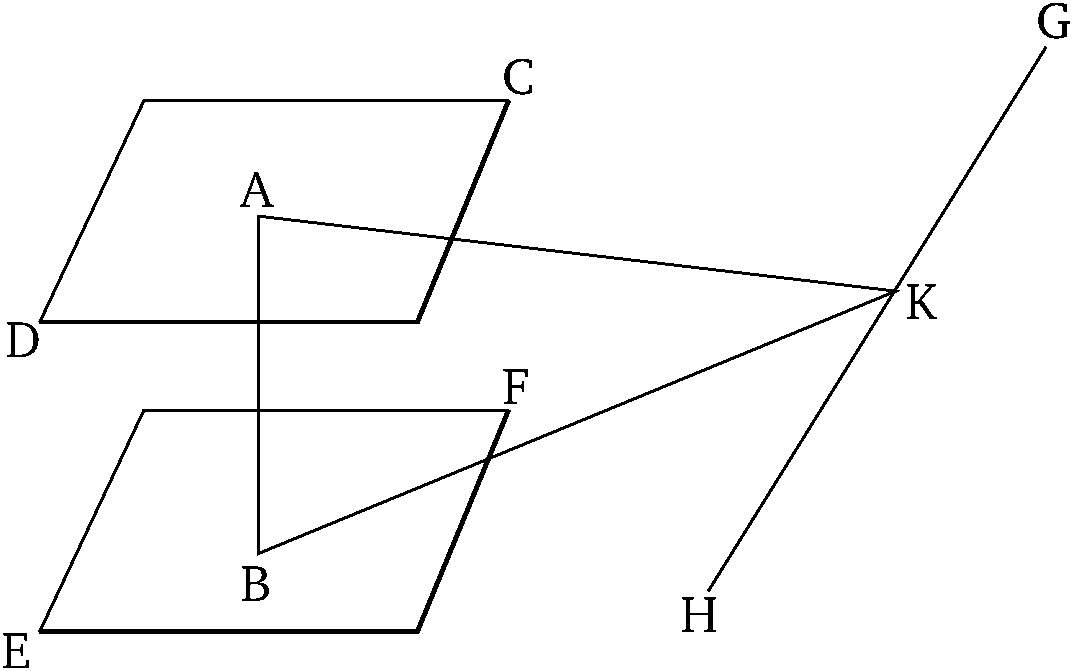
\includegraphics{Book11/fig14e.eps}}

For, if not, being produced, they will meet. Let them have
met. So they will make a straight-line as a common section [Prop.~11.3]. Let them have made $GH$. And let some
random point $K$ be taken on $GH$. And let $AK$ and
$BK$ be joined.

And since $AB$ is at right-angles to the plane $EF$, $AB$ is thus also
at right-angles to  $BK$, which is a straight-line in the produced plane $EF$ [Def.~11.3]. 
Thus, angle $ABK$ is a right-angle.
So, for the same (reasons), $BAK$ is also a right-angle. So the (sum of the)
two angles $ABK$ and $BAK$ in the triangle $ABK$ is equal to
two right-angles. The very thing is impossible [Prop.~1.17]. Thus, planes $CD$ and $EF$, being produced, will not meet.
Planes $CD$ and $EF$ are thus parallel [Def.~11.8].

Thus, planes to which the same straight-line
is at right-angles are  parallel planes. (Which is) the very thing it was required to show.}
\end{Parallel}

%%%%
%11.15
%%%%
\pdfbookmark[1]{Proposition 11.15}{pdf11.15}
\begin{Parallel}{}{}
\ParallelLText{
\begin{center}
{\large \ggn{15}.}
\end{center}\vspace*{-7pt}

\gr{Ἐὰν δύο εὐθεῖαι ἁπτόμεναι ἀλλήλων παρὰ δύο εὐθείαξ ἁπτομέναξ
ἀλλήλων >ῶσι μ\kern -.7pt  ὴ ἐν τῶ| α\kern -.7pt  ὐτῶ| ἐπιπέδῳ ο>ῦσαι, παράλληλά
ἐστι τὰ δι> α\kern -.5pt  ὐτῶν ἐπίπεδα.}

\gr{Δύο γὰρ εὐθεῖαι ἁπτόμεναι ἀλλήλων αἱ ΑΒ, ΒΓ παρὰ δύο εὐθείαξ
ἁπτομέναξ ἀλλήλων τὰξ ΔΕ, ΕΖ >έστωσαν μ\kern -.7pt  ὴ ἐν τῶ| α\kern -.7pt  ὐτῶ|
ἐπιπέδῳ ο>ῦσαι; λέγω, <ότι ἐκβαλλόμενα τὰ διὰ τῶν
ΑΒ, ΒΓ, ΔΕ, ΕΖ ἐπίπεδα οὐ συμπεσεῖται ἀλλήλοιξ.}

\gr{>'Ηθθω γὰρ ἀπὸ τοῦ Β σημείου ἐπὶ τὸ διὰ τῶν ΔΕ, ΕΖ
ἐπίπεδον κάθετοξ ἡ ΒΗ καὶ συμβαλλέτω τῶ| ἐπιπέδῳ
κατὰ τὸ Η σημεῖον, καὶ διὰ τοῦ Η τῆ| μὲν ΕΔ παράλληλοξ
>ήθθω ἡ ΗJ, τῆ| δὲ ΕΖ ἡ ΗΚ.}\\~\\

\epsfysize=2.2in
\centerline{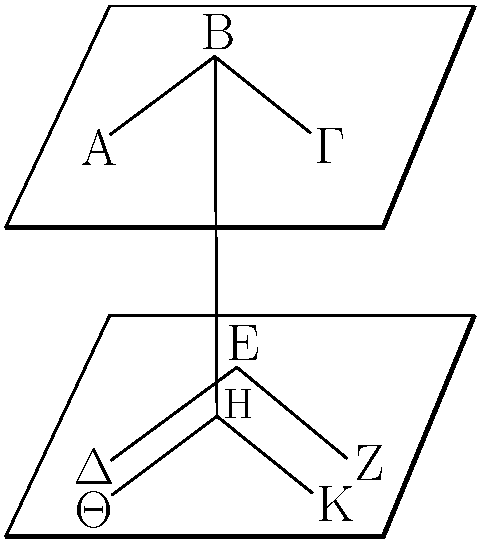
\includegraphics{Book11/fig15g.eps}}

\gr{Καὶ ἐπεὶ ἡ ΒΗ ὀρθή ἐστι
πρὸξ τὸ διὰ τῶν ΔΕ, ΕΖ ἐπίπεδον, καὶ πρὸξ πάσαξ
>άρα τὰξ ἁπτομέναξ α\kern -.7pt  ὐτῆξ εὐθείαξ καὶ ο>ύσαξ ἐν τῶ| διὰ τῶν
ΔΕ, ΕΖ ἐπιπέδῳ ὀρθὰξ ποιήσει γωνίαξ. <άπτεται δὲ α\kern -.7pt  ὐτῆξ
ἑκατέρα τῶν ΗJ, ΗΚ ο>ῦσα ἐν τῶ| διὰ τῶν ΔΕ, ΕΖ ἐπιπέδῳ;
ὀρθὴ >άρα ἐστὶν ἑκατέρα τῶν ὑπὸ ΒΗJ, ΒΗΚ γωνιῶν. καὶ
ἐπεὶ παράλληλόξ ἐστιν ἡ ΒΑ τῆ| ΗJ, αἱ >άρα ὑπὸ ΗΒΑ, ΒΗJ
γωνίαι δυσὶν ὀρθαῖξ >ίσαι εἰσίν.
ὀρθὴ δὲ ἡ ὑπὸ ΒΗJ; ὀρθὴ >άρα καὶ ἡ ὑπὸ ΗΒΑ; ἡ ΗΒ
>άρα τῆ| ΒΑ πρὸξ ὀρθάξ ἐστιν. διὰ τὰ α\kern -.5pt  ὐτὰ δὴ ἡ ΗΒ
 καὶ τῆ| ΒΓ ἐστι πρὸξ ὀρθάξ. ἐπεὶ ο>ῦν εὐθεῖα ἡ ΗΒ
δυσὶν εὐθείαιξ ταῖξ ΒΑ, ΒΓ τεμνούσαιξ ἀλλήλαξ πρὸξ ὀρθὰξ
ἐφέστηκεν, ἡ ΗΒ >άρα καὶ τῶ| διὰ τῶν ΒΑ, ΒΓ ἐπιπέδῳ
πρὸξ ὀρθάξ ἐστιν. [διὰ τὰ α\kern -.3pt  ὐτὰ δὴ ἡ ΒΗ καὶ τῶ| διὰ τῶν
ΗJ, ΗΚ ἐπιπέδῳ πρὸξ ὀρθάξ ἐστιν. τὸ δὲ διὰ τῶν ΗJ, ΗΚ
ἐπίπεδόν ἐστι τὸ διὰ τῶν ΔΕ, ΕΖ; ἡ ΒΗ >άρα τῶ| διὰ τῶν
ΔΕ, ΕΖ ἐπιπέδῳ ἐστὶ πρὸξ ὀρθάξ. ἐδείθθη
δὲ ἡ ΗΒ καὶ τῶ| διὰ τῶν ΑΒ, ΒΓ ἐπιπέδῳ πρὸξ
ὀρθάξ]. πρὸξ <ὰ δὲ ἐπίπεδα ἡ α\kern -.7pt  ὐτὴ εὐθεῖα ὀρθή
ἐστιν, παράλληλά ἐστι τὰ ἐπίπεδα; παράλληλον >άρα ἐστὶ τὸ διὰ
τῶν ΑΒ, ΒΓ ἐπίπεδον τῶ| διὰ τῶν ΔΕ, ΕΖ.}

\gr{Ἐὰν >άρα δύο εὐθεῖαι ἁπτόμεναι ἀλλήλων παρὰ δύο εὐθείαξ ἁπτομέναξ
ἀλλήλων >ῶσι μ\kern -.7pt  ὴ ἐν τῶ| α\kern -.7pt  ὐτῶ| ἐπιπέδῳ, παράλληλά
ἐστι τὰ δι> α\kern -.5pt  ὐτῶν ἐπίπεδα; <όπερ >έδει δεῖχαι.}}

\ParallelRText{
\begin{center}
{\large Proposition 15}
\end{center}

If two straight-lines joined to one another
are parallel (respectively) to two straight-lines joined to one another, which
are not in the same plane,
then the planes through them are parallel (to one another).

For let the two straight-lines joined to one another, $AB$ and $BC$, be parallel to the two straight-lines joined to one another, $DE$ and $EF$ (respectively), not being in the same plane. I say that the planes
through $AB$, $BC$ and $DE$, $EF$ will not meet one another (when) produced.

For let $BG$ be drawn from point $B$ perpendicular to the
plane through $DE$ and $EF$ [Prop.~11.11], and
let it meet the plane at point $G$. And let $GH$ be drawn through
$G$ parallel to $ED$, and $GK$ (parallel) to $EF$ [Prop.~1.31].

\epsfysize=2.2in
\centerline{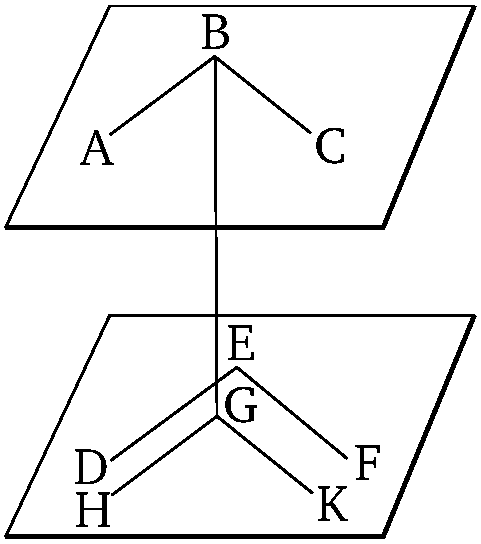
\includegraphics{Book11/fig15e.eps}}

And since $BG$ is at right-angles to the plane through $DE$ and $EF$,
it will thus also make right-angles with all of the straight-lines joined to it, which
are also in the plane through $DE$ and $EF$ [Def.~11.3]. And each of $GH$ and
$GK$, which are in the plane through $DE$ and $EF$,  are joined to it. 
Thus, each of the angles $BGH$ and $BGK$ are right-angles. And since
$BA$ is parallel to $GH$ [Prop.~11.9], the (sum of the) angles $GBA$ and $BGH$
is equal to two right-angles [Prop.~1.29]. 
And $BGH$ (is) a right-angle. $GBA$ (is) thus also a right-angle.
Thus, $GB$ is at right-angles to $BA$. So, for the same (reasons), $GB$
is also at right-angles to $BC$. Therefore, since the straight-line $GB$
has been set up at right-angles to two straight-lines, $BA$ and $BC$, cutting
one another, $GB$ is thus at right-angles to the plane through $BA$ and
$BC$ [Prop.~11.4]. [So, for the same (reasons), $BG$ is also at right-angles to the plane through $GH$ and $GK$. And the plane
through $GH$ and $GK$ is the (plane) through $DE$ and $EF$. And it was also shown that $GB$ is at right-angles to the plane through $AB$ and
$BC$.] And planes to which the same straight-line is at right-angles are
parallel planes [Prop.~11.14]. Thus, the plane
through $AB$ and $BC$ is parallel to the (plane) through $DE$ and $EF$.

Thus, if two straight-lines joined to one another
are parallel (respectively) to two straight-lines joined to one another, which
are not in the same plane,
then the planes through them are parallel (to one another). (Which is) the very thing it was required to show.}
\end{Parallel}

%%%%
%11.16
%%%%
\pdfbookmark[1]{Proposition 11.16}{pdf11.16}
\begin{Parallel}{}{}
\ParallelLText{
\begin{center}
{\large \ggn{16}.}
\end{center}\vspace*{-7pt}

\gr{Ἐὰν δύο ἐπίπεδα παράλληλα ὑπὸ ἐπιπέδου τινὸξ τέμνηται, αἱ
κοιναὶ α\kern -.7pt  ὐτῶν τομαὶ παράλληλοί εἰσιν.}

\gr{Δύο γὰρ ἐπίπεδα παράλληλα τὰ ΑΒ, ΓΔ ὑπὸ ἐπιπέδου τοῦ ΕΖΗJ
τεμνέσθω, κοιναὶ δὲ α\kern -.7pt  ὐτῶν τομαὶ >έστωσαν αἱ ΕΖ, ΗJ;
λέγω, <ότι παράλληλόξ ἐστιν ἡ ΕΖ τῆ| ΗJ.}

\gr{Εἰ γὰρ μ\kern -.7pt  ή, ἐκβαλλόμεναι αἱ ΕΖ, ΗJ >ήτοι ἐπὶ τὰ Ζ, J μέρη >ὴ
ἐπὶ τὰ Ε, Η συμπεσοῦνται. ἐκβεβλήσθωσαν ὡξ ἐπὶ τὰ
Ζ, J μέρη καὶ συμπιπτέτωσαν πρότερον κατὰ τὸ Κ. καὶ ἐπεὶ
ἡ ΕΖΚ ἐν τῶ| ΑΒ ἐστιν ἐπιπέδῳ, καὶ πάντα >άρα τὰ ἐπὶ 
τῆξ ΕΖΚ σημεῖα ἐν τῶ| ΑΒ ἐστιν ἐπιπέδῳ. <ὲν δὲ τῶν 
ἐπὶ τῆξ ΕΖΚ εὐθείαξ σημείων ἐστὶ τὸ Κ; τὸ Κ >άρα ἐν τῶ|
ΑΒ ἐστιν ἐπιπέδῳ. διὰ  τὰ α\kern -.7pt  ὐτὰ δὴ τὸ Κ καὶ ἐν τῶ| ΓΔ 
ἐστιν ἐπιπέδῳ; τὰ ΑΒ, ΓΔ >άρα ἐπίπεδα ἐκβαλλόμενα συμπεσοῦνται.
οὐ συμπίπτουσι δὲ διὰ τὸ παράλληλα ὑποκεῖσθαι; οὐκ >άρα αἱ 
ΕΖ, ΗJ εὐθεῖαι ἐκβαλλόμεναι  ἐπὶ τὰ Ζ, J μέρη συμπεσοῦνται.
ὁμοίωξ δὴ δείχομεν, <ότι αἱ ΕΖ, ΗJ εὐθεῖαι  οὐδέ ἐπὶ 
τὰ Ε, Η μέρη ἐκβαλλόμεναι συμπεσοῦνται. αἱ δὲ ἐπὶ μ\kern -.5pt  ηδέτερα 
τὰ μέρη συμπίπτουσαι παράλληλοί εἰσιν. παράλληλοξ >άρα 
ἐστὶν  ἡ ΕΖ τῆ| ΗJ.}\\

\epsfysize=2.in
\centerline{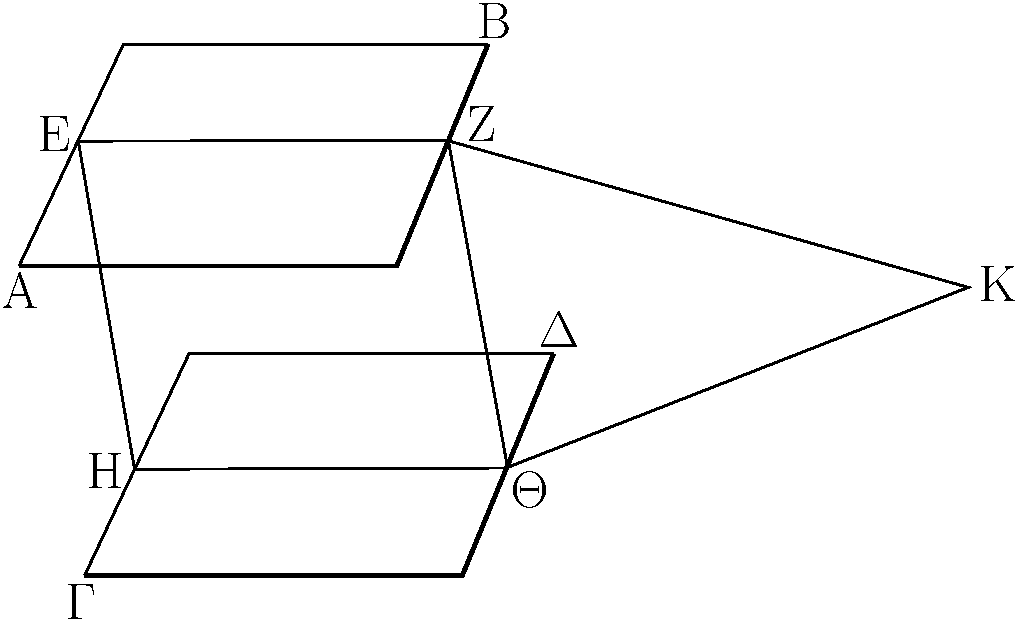
\includegraphics{Book11/fig16g.eps}}

\gr{Ἐὰν >άρα δύο ἐπίπεδα παράλληλα ὑπὸ ἐπιπέδου τινὸξ τέμνηται, αἱ
κοιναὶ α\kern -.7pt  ὐτῶν τομαὶ παράλληλοί εἰσιν; <όπερ >έδει δεῖχαι.}}

\ParallelRText{
\begin{center}
{\large Proposition 16}
\end{center}

If two parallel planes are cut by some plane
then their common sections are parallel.

For let the two parallel planes $AB$ and $CD$ be cut by the
plane $EFGH$. And let $EF$ and $GH$ be their common sections.
I say that $EF$ is parallel to $GH$.

For, if not, being produced, $EF$ and $GH$ will  meet either in the direction of $F$, $H$, 
 or of $E$, $G$. Let them  be produced, as  in the  direction of $F$, $H$, and let them, first of all, have met at $K$. And since $EFK$ is in the plane $AB$, all
 of the points on $EFK$ are thus also in the plane $AB$ [Prop.~11.1]. And $K$ is one of the points on $EFK$. Thus, $K$ is in the
 plane $AB$. So, for the same (reasons), $K$ is also in the plane $CD$. 
 Thus, the planes $AB$ and $CD$, being produced, will meet. But they do
 not meet, on account of being (initially) assumed (to be mutually) parallel. Thus,
 the straight-lines $EF$ and $GH$, being produced in the
direction of $F$, $H$, will not meet. So, similarly, we can show that the straight-lines
 $EF$ and $GH$, being produced in the direction of $E$, $G$, will not meet
 either. And (straight-lines in one plane which), being produced,  do not meet in either direction
 are parallel [Def.~1.23]. $EF$ is thus parallel to $GH$.

\epsfysize=2.in
\centerline{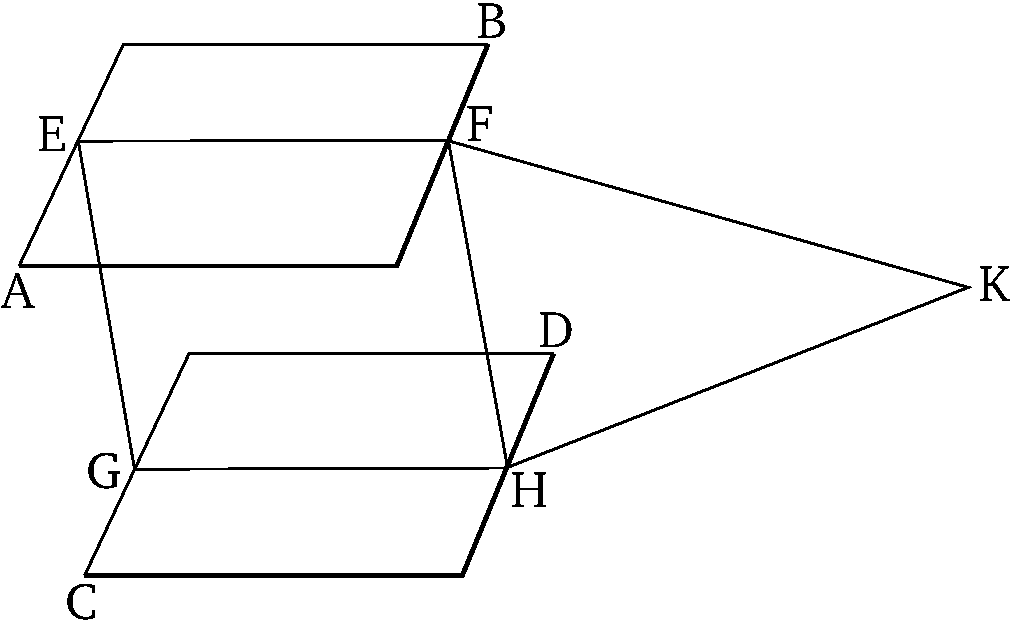
\includegraphics{Book11/fig16e.eps}}
 
 Thus, if two parallel planes are cut by some plane
then their common sections are parallel. (Which is) the very thing it was
required to show.}
\end{Parallel}

%%%%
%11.17
%%%%
\pdfbookmark[1]{Proposition 11.17}{pdf11.17}
\begin{Parallel}{}{}
\ParallelLText{
\begin{center}
{\large \ggn{17}.}
\end{center}\vspace*{-7pt}

\gr{Ἐὰν δύο εὐθεῖαι ὑπὸ παραλλήλων ἐπιπεδων τέμνωνται, εἰξ
τοὺξ α\kern -.7pt  ὐτοὺξ λόγουξ τμ\kern -.7pt  ηθήσονται.}

\gr{Δύο γὰρ εὐθεῖαι αἱ ΑΒ, ΓΔ ὑπὸ παραλλήλων ἐπιπέδων τῶν ΗJ, ΚΛ,
ΜΝ τεμνέσθωσαν κατὰ τὰ Α, Ε, Β, Γ, Ζ, Δ σημεῖα; λέγω, <ότι ἐστὶν
ὡξ ἡ ΑΕ εὐθεῖα πρὸξ τὴν  ΕΒ, ο<ύτωξ ἡ ΓΖ πρὸξ τὴν ΖΔ.}

\gr{Ἐπεζεύθθωσαν γὰρ αἱ ΑΓ, ΒΔ, ΑΔ, καὶ συμβαλλέτω ἡ ΑΔ τῶ| ΚΛ
ἐπιπέδῳ κατὰ τὸ Χ σημεῖον, καὶ ἐπεζεύθθωσαν αἱ ΕΧ, ΧΖ.}

\gr{Καὶ ἐπεὶ δύο ἐπίπεδα παράλληλα τὰ ΚΛ, ΜΝ ὑπὸ ἐπιπέδου
τοῦ ΕΒΔΧ τέμνεται, αἱ κοιναὶ α\kern -.7pt  ὐτῶν τομαὶ αἱ ΕΧ, ΒΔ
παράλληλοί εἰσιν. διὰ τὰ α\kern -.7pt  ὐτὰ δὴ ἐπεὶ δύο ἐπίπεδα 
παράλληλα τὰ ΗJ, ΚΛ ὑπὸ ἐπιπέδου τοῦ ΑΧΖΓ τέμνεται, αἱ 
κοιναὶ α\kern -.5pt  ὐτῶν τομαὶ αἱ ΑΓ, ΧΖ παράλληλοί εἰσιν. καὶ ἐπεὶ
τριγώνου τοῦ ΑΒΔ παρὰ μίαν τῶν πλευρῶν τὴν ΒΔ εὐθεῖα
>ῆκται ἡ ΕΧ, ἀνάλογον >άρα ἐστὶν ὡξ ἡ ΑΕ πρὸξ ΕΒ, ο<ύτωξ
ἡ ΑΧ πρὸξ ΧΔ. πάλιν ἐπεὶ τριγώνου τοῦ ΑΔΓ παρὰ μίαν 
τῶν πλευρῶν τὴν ΑΓ εὐθεῖα >ῆκται ἡ ΧΖ, ἀνάλογόν 
ἐστιν ὡξ ἡ ΑΧ πρὸξ ΧΔ, ο<ύτωξ ἡ ΓΖ πρὸξ ΖΔ. ἐδείθθη
δὲ καὶ ὡξ ἡ ΑΧ πρὸξ ΧΔ, ο<ύτωξ ἡ ΑΕ πρὸξ ΕΒ; καὶ ὡξ
>άρα ἡ ΑΕ πρὸξ ΕΒ, ο<ύτωξ ἡ ΓΖ πρὸξ ΖΔ.}

\epsfysize=3in
\centerline{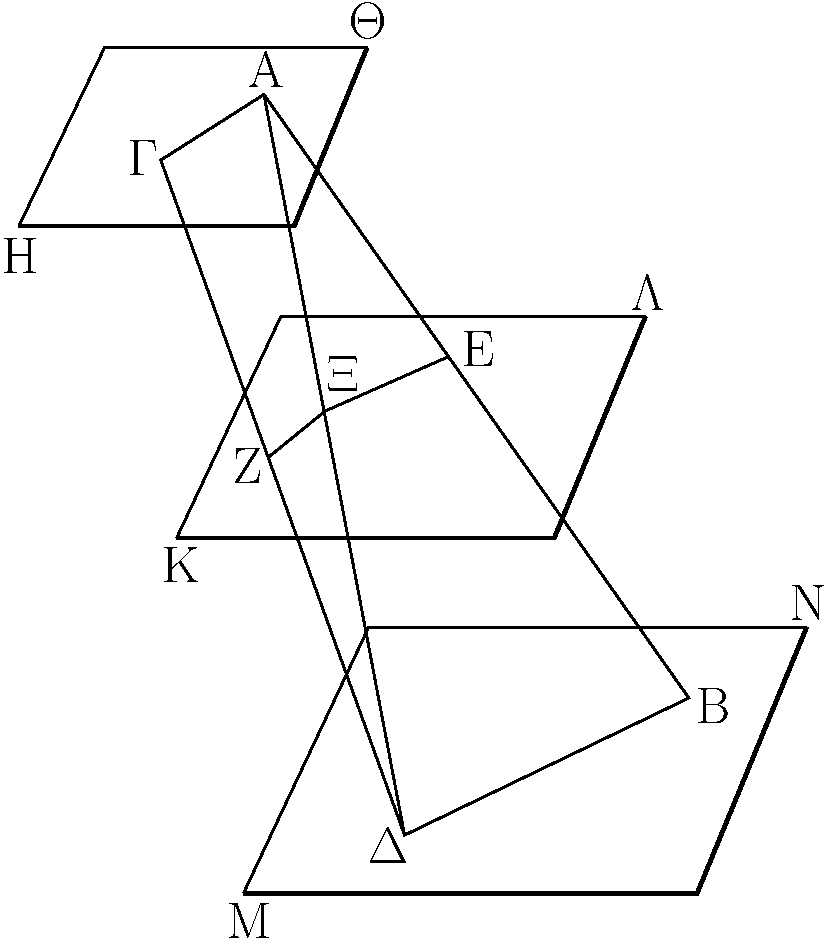
\includegraphics{Book11/fig17g.eps}}

\gr{Ἐὰν >άρα δύο εὐθεῖαι ὑπὸ παραλλήλων ἐπιπέδων τέμνων\-ται,
εἰξ τοὺξ α\kern -.7pt  ὐτοὺξ λόγουξ τμ\kern -.7pt  ηθήσονται; <όπερ >έδει δειχαι.}}

\ParallelRText{

\begin{center}
{\large Proposition 17}
\end{center}

If two straight-lines are cut by parallel planes then
they will be cut in the same ratios.

For let the two straight-lines $AB$ and $CD$ be cut by the parallel planes
$GH$, $KL$, and $MN$ at the points $A$, $E$, $B$,  and $C$, $F$, $D$ (respectively). I say that as the straight-line $AE$ is to $EB$, so $CF$ (is)
to $FD$.

For let $AC$, $BD$, and $AD$ be joined, and let $AD$ meet the
plane $KL$ at point $O$, and let $EO$ and $OF$ be joined.

And since two parallel planes $KL$ and $MN$ are cut by the
plane $EBDO$, their common sections $EO$ and $BD$ are parallel
[Prop.~11.16]. So, for the same (reasons), 
since two parallel planes $GH$ and $KL$ are cut by the plane
$AOFC$, their common sections $AC$ and $OF$ are 
parallel [Prop.~11.16]. And since the straight-line $EO$ has been drawn parallel to
one of the sides $BD$ of triangle $ABD$, thus, proportionally, as 
$AE$ is to $EB$, so $AO$ (is) to $OD$ [Prop.~6.2]. 
Again, since the straight-line $OF$ has been drawn parallel to one of the sides $AC$
of triangle $ADC$, proportionally, as $AO$ is to $OD$, so $CF$ (is) to $FD$ [Prop.~6.2]. And it was also shown that as $AO$ (is) to $OD$, so $AE$ (is) to $EB$.
And thus as $AE$ (is) to $EB$, so $CF$ (is) to $FD$ [Prop.~5.11].\\

\epsfysize=3in
\centerline{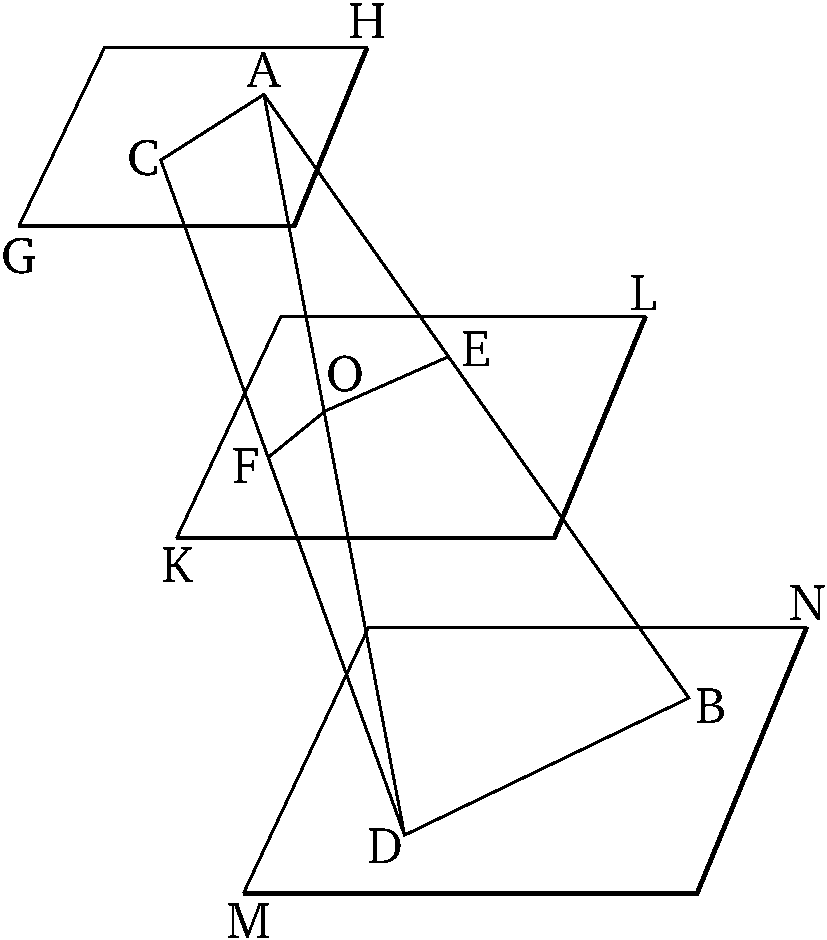
\includegraphics{Book11/fig17e.eps}}

Thus, if two straight-lines are cut by parallel planes then
they will be cut in the same ratios. (Which is) the very thing it was required to
show.}
\end{Parallel}

%%%%
%11.18
%%%%
\pdfbookmark[1]{Proposition 11.18}{pdf11.18}
\begin{Parallel}{}{}
\ParallelLText{ 
\begin{center}
{\large \ggn{18}.}
\end{center}\vspace*{-7pt}

\gr{Ἐὰν εὐθεῖα ἐπιπέδῳ τινὶ πρὸξ ὀρθὰξ >ῆ|,
καὶ πάντα τὰ δι> α\kern -.7pt  ὐτῆξ ἐπίπεδα τῶ| α\kern -.7pt  ὐτῶ| ἐπιπέδῳ
πρὸξ ὀρθὰξ >έσται.}

\gr{Εὐθεῖα γάρ τιξ ἡ ΑΒ τῶ| ὑποκειμένῳ ἐπιπέδῳ
πρὸξ ὀρθὰξ >έστω; λέγω, <ότι καὶ πάντα τὰ διὰ τῆξ ΑΒ ἐπίπεδα
τῶ| ὑποκειμένῳ ἐπιπέδῳ πρὸξ ὀρθάξ ἐστιν.}

\gr{Ἐκβεβλήσθω γὰρ διὰ τῆξ ΑΒ ἐπίπεδον τὸ ΔΕ,
καὶ >έστω κοινὴ τομ\kern -.7pt  ὴ τοῦ ΔΕ ἐπιπέδου καὶ τοῦ ὑποκειμένου
ἡ ΓΕ, καὶ εἰλήφθω ἐπὶ τῆξ ΓΕ τυθὸν σημεῖον τὸ Ζ, καὶ ἀπὸ
τοῦ Ζ τῆ| ΓΕ πρὸξ ὀρθὰξ >ήθθω ἐν τῶ| ΔΕ ἐπιπέδῳ ἡ ΖΗ.}

\gr{Καὶ ἐπεὶ ἡ ΑΒ πρὸξ τὸ ὑποκείμενον ἐπίπεδον ὀρθή
ἐστιν, καὶ πρὸξ πάσαξ >άρα τὰξ ἁπτομέναξ α\kern -.7pt  ὐτῆξ εὐθείαξ
καὶ ο>ύσαξ ἐν τῶ| ὑποκειμένῳ ἐπιπέδῳ ὀρθή
ἐστιν ἡ ΑΒ; <ώστε καὶ πρὸξ τὴν ΓΕ ὀρθή ἐστιν; ἡ >άρα ὑπὸ
ΑΒΖ γωνία ὀρθή ἐστιν. >έστι δὲ καὶ ἡ ὑπὸ ΗΖΒ ὀρθὴ;
παράλληλοξ  >άρα ἐστὶν ἡ ΑΒ τῆ| ΖΗ. ἡ δὲ ΑΒ τῶ| ὑποκειμένῳ
ἐπιπέδῳ πρὸξ ὀρθάξ ἐστιν; καὶ ἡ ΖΗ >άρα τῶ| ὑποκειμένῳ
ἐπιπέδῳ πρὸξ ὀρθάξ ἐστιν. καὶ
 ἐπίπεδον πρὸξ ἐπίπεδον ὀρθόν ἐστιν, <όταν αἱ τῆ| κοινῆ|
 τομ\kern -.7pt  ῆ| τῶν ἐπιπέδων πρὸξ ὀρθὰξ ἀγόμεναι εὐθεῖαι ἐν ἑνὶ
 τῶν ἐπιπέδων τῶ| λοιπῶ| ἐπιπέδῳ πρὸξ ὀρθὰξ >ῶσιν.
 καὶ τῆ| κοινῆ| τομ\kern -.5pt  ῆ| τῶν ἐπιπέδων τῆ| ΓΕ ἐν ἑνὶ τῶν
 ἐπιπέδων τῶ| ΔΕ πρὸξ ὀρθὰξ ἀθθεῖσα ἡ ΖΗ ἐδείθθη
 τῶ| ὑποκειμένῳ ἐπιπέδῳ πρὸξ ὀρθάξ; τὸ >άρα ΔΕ ἐπίπεδον
 ὀρθόν ἐστι πρὸξ τὸ ὑποκείμενον. ὁμοίωξ δὴ δειθθήσεται
 καὶ πάντα τὰ διὰ τῆξ ΑΒ ἐπίπεδα ὀρθὰ τυγθανοντα πρὸξ τὸ ὑποκείμενον ἐπίπεδον.}\\~\\~\\~\\

\epsfysize=2.in
\centerline{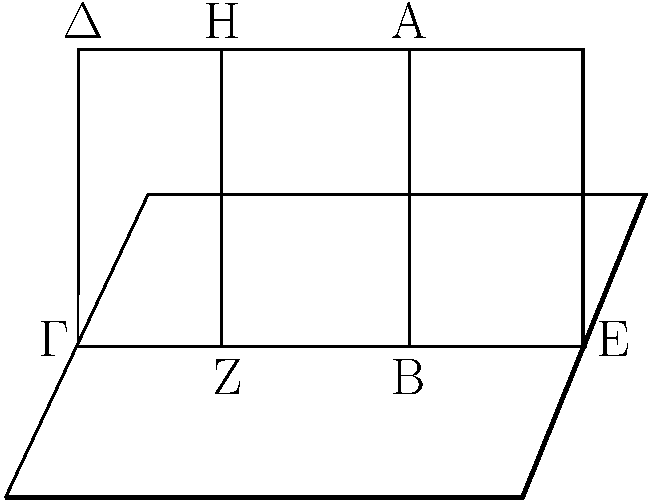
\includegraphics{Book11/fig18g.eps}}

\gr{Ἐὰν >άρα εὐθεῖα ἐπιπέδῳ τινὶ πρὸξ ὀρθὰξ >ῆ|, καὶ πάντα τὰ
 δι> α\kern -.7pt  ὐτῆξ ἐπίπεδα τῶ| α\kern -.7pt  ὐτῶ| ἐπιπέδῳ πρὸξ ὀρθὰξ >έσται;
 <όπερ >έδει δεῖχαι.}}
 
\ParallelRText{
\begin{center}
{\large Proposition 18}
\end{center}

If a straight-line is at right-angles to some plane then all of the planes (passing) through it will also be at right-angles to the same
plane.

For let some straight-line $AB$ be at right-angles to a reference plane.
I say that all of the planes (passing) through $AB$ are also at right-angles to 
the reference plane.

For let the plane $DE$ be produced through $AB$. And let $CE$
be the common section of the plane $DE$ and the reference (plane).
And let some random point $F$ be taken on $CE$. And let
$FG$ be drawn from $F$, at right-angles to $CE$, in the plane $DE$
[Prop.~1.11].

And since $AB$ is at right-angles to the reference plane, $AB$ is thus also
at right-angles to all of the straight-lines joined to it which are also in the reference
plane [Def.~11.3]. Hence, it is also at right-angles to
$CE$. Thus, angle $ABF$ is a right-angle. And $GFB$ is also a right-angle.
Thus, $AB$ is parallel to $FG$ [Prop.~1.28].
And $AB$ is at right-angles to the reference plane. Thus, $FG$ is also
at right-angles to the reference plane [Prop.~11.8].
And a plane is at right-angles to a(nother) plane when the straight-lines drawn at
right-angles to the common section
of the planes,  (and lying) in one of the planes,
are at right-angles to the remaining plane [Def.~11.4].
And $FG$, (which was) drawn  at right-angles to the common
section of the planes, $CE$, in one of the planes, $DE$,  was shown  to be at right-angles to the reference plane. Thus, plane $DE$ is at right-angles
to the reference (plane). So, similarly, it can be shown that   all of the planes
(passing) at random through $AB$ (are) at right-angles to the
reference plane.

\epsfysize=2.in
\centerline{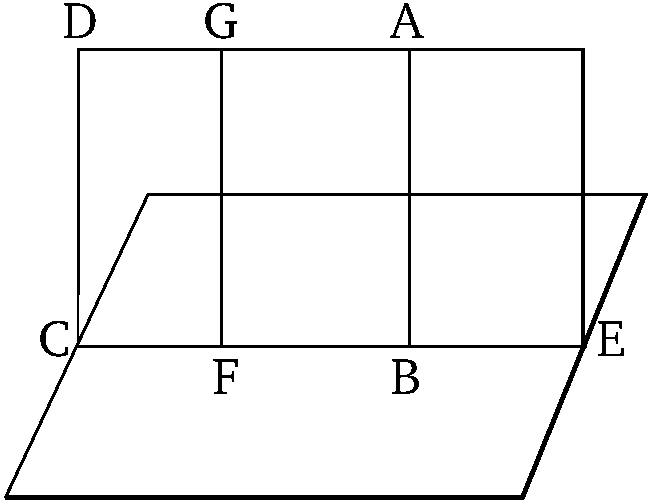
\includegraphics{Book11/fig18e.eps}}

Thus, if  a straight-line is at right-angles to some plane then all of the planes (passing) through it will also be at right-angles to the same
plane. (Which is) the very thing it was required to show.}
\end{Parallel}

%%%%
%11.19
%%%%
\pdfbookmark[1]{Proposition 11.19}{pdf11.19}
\begin{Parallel}{}{}
\ParallelLText{
\begin{center}
{\large \ggn{19}.}
\end{center}\vspace*{-7pt}

\gr{Ἐὰν δύο ἐπίπεδα τέμνοντα >άλληλα ἐπιπέδῳ τινὶ πρὸξ ὀρθὰξ >ῆ|,
καὶ ἡ κοινὴ α\kern -.7pt  ὐτῶν τομ\kern -.7pt  ὴ τῶ| α\kern -.5pt  ὐτῶ| ἐπιπέδῳ πρὸξ ὀρθὰξ
>έσται.}

\epsfysize=2.2in
\centerline{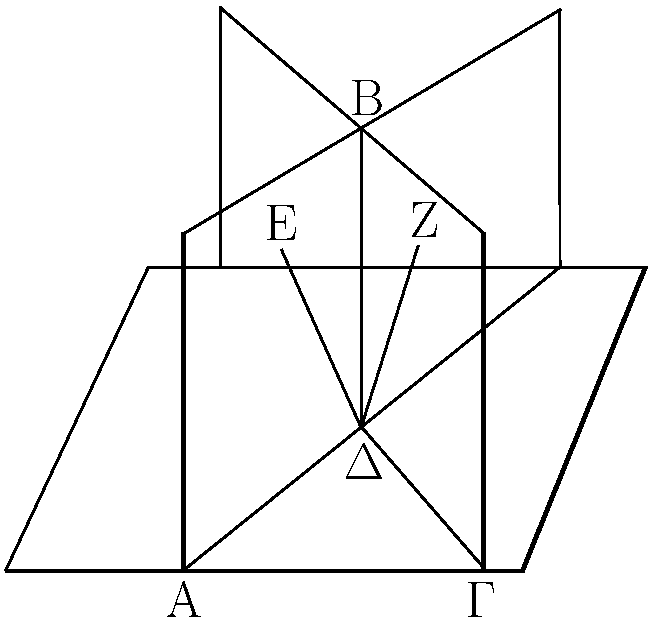
\includegraphics{Book11/fig19g.eps}}

\gr{Δύο γὰρ ἐπίπεδα τὰ ΑΒ, ΒΓ τῶ| ὑποκειμένῳ ἐπιπέδῳ πρὸξ
ὀρθὰξ >έστω, κοινὴ δὲ α\kern -.7pt  ὐτῶν τομ\kern -.7pt  ὴ >έστω ἡ ΒΔ;
λέγω, <ότι ἡ ΒΔ τῶ| ὑποκειμένῳ ἐπιπέδῳ πρὸξ ὀρθάξ ἐστιν.}

\gr{μ\kern -.7pt  ὴ γάρ, καὶ >ήθθωσαν ἀπὸ τοῦ Δ σημείου ἐν μὲν τῶ| ΑΒ ἐπιπέδῳ τῆ| ΑΔ εὐθείᾳ πρὸξ ὀρθὰξ ἡ ΔΕ, ἐν δὲ τῶ| ΒΓ ἐπιπέδῳ τῆ| ΓΔ πρὸξ ὀρθὰξ ἡ ΔΖ.}

\gr{Καὶ ἐπεὶ τὸ ΑΒ ἐπίπεδον
ὀρθόν ἐστι πρὸξ τὸ ὑποκείμενον, καὶ τῆ| κοινῆ| α\kern -.7pt  ὐτῶν
τομ\kern -.7pt  ῆ| τῆ| ΑΔ πρὸξ ὀρθὰξ ἐν τῶ| ΑΒ ἐπιπέδῳ >ῆκται ἡ ΔΕ, ἡ
ΔΕ >άρα ὀρθή ἐστι πρὸξ τὸ ὑποκείμενον ἐπίπεδον. ὁμοίωξ
δὴ δείχομεν, <ότι καὶ ἡ ΔΖ ὀρθή ἐστι πρὸξ τὸ ὑποκείμενον
ἐπίπεδον. ἀπὸ τοῦ α\kern -.5pt  ὐτοῦ >άρα σημείου τοῦ Δ τῶ| ὑποκειμένῳ
ἐπιπέδῳ δύο εὐθεῖα πρὸξ ὀρθὰξ ἀνεσταμέναι εἰσὶν ἐπὶ
τὰ α\kern -.3pt  ὐτὰ μέρη; <όπερ ἐστὶν ἀδύνατον. οὐκ >άρα τῶ| ὑποκειμένῳ
ἐπιπέδῳ ἀπὸ τοῦ Δ σημείου ἀνασταθήσεται πρὸξ ὀρθὰξ πλὴν
τῆξ ΔΒ κοινῆξ τομ\kern -.7pt  ῆξ τῶν ΑΒ, ΒΓ ἐπιπέδων.}

\gr{Ἐὰν >άρα δύο ἐπίπεδα τέμνοντα >άλληλα ἐπιπέδῳ τινὶ πρὸξ ὀρθὰξ >ῆ|,
καὶ ἡ κοινὴ α\kern -.7pt  ὐτῶν τομ\kern -.7pt  ὴ τῶ| α\kern -.5pt  ὐτῶ| ἐπιπέδῳ πρὸξ ὀρθὰξ
>έσται; <όπερ >έδει δεῖχαι.}}

\ParallelRText{
\begin{center}
{\large Proposition 19}
\end{center}

If two planes cutting one another are at right-angles to some plane then their common section will also be at right-angles to the
same plane.

\epsfysize=2.2in
\centerline{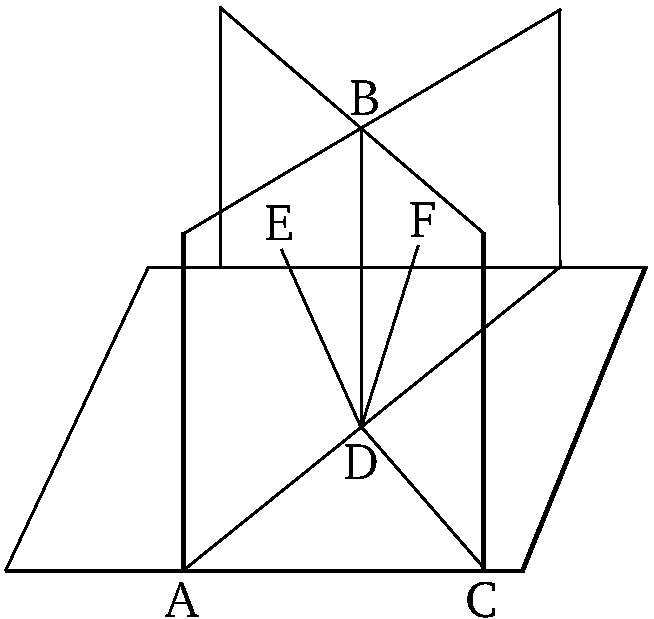
\includegraphics{Book11/fig19e.eps}}

For let the two planes $AB$ and $BC$ be at right-angles to a reference
plane, and let their common section be $BD$. I say that $BD$ is at right-angles to the reference plane.

For (if) not, let $DE$ also be drawn from point $D$,  in the plane
$AB$, at right-angles to the straight-line $AD$, and $DF$, in the plane $BC$, at right-angles to $CD$.

And since the plane $AB$ is at right-angles to the reference (plane),
and $DE$ has been drawn at right-angles to their common section $AD$,
in the plane $AB$, $DE$ is thus at right-angles to the reference 
plane [Def.~11.4]. So, similarly, we can show that
$DF$ is also at right-angles to the reference plane. Thus, two (different) straight-lines
are set up, at the same point $D$, at right-angles to the reference plane,
on the same side. The very thing is impossible [Prop.~11.13]. Thus, no (other straight-line) except the common section
$DB$ of the planes $AB$ and $BC$ can be set up at point $D$,
at right-angles to the reference plane.

Thus, if two planes cutting one another are at right-angles to some plane then their common section will also be at right-angles to the
same plane. (Which is) the very thing it was required to show.}
\end{Parallel}

%%%%
%11.20
%%%%
\pdfbookmark[1]{Proposition 11.20}{pdf11.20}
\begin{Parallel}{}{}
\ParallelLText{
\begin{center}
{\large\ggn{20}.}
\end{center}\vspace*{-7pt}

\gr{Ἐὰν στερεὰ γωνία ὑπὸ τριῶν γωνιῶν ἐπιπέδων περιέθη\-ται, δύο
ὁποιαιοῦν τῆξ λοιπῆξ μείζονέξ εἰσι πάντῃ μεταλαμβανόμεναι.}

\epsfysize=1.5in
\centerline{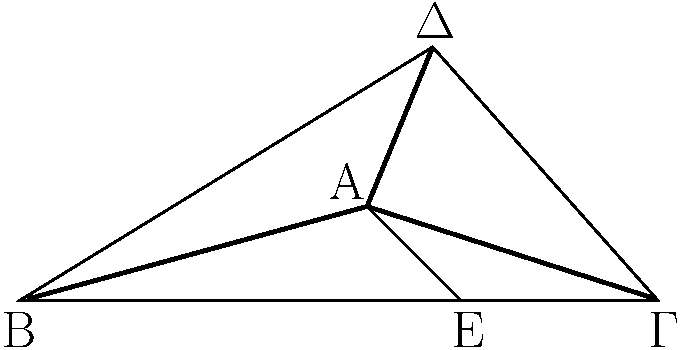
\includegraphics{Book11/fig20g.eps}}

\gr{Στερεὰ γὰρ γωνία ἡ πρὸξ τῶ| Α ὑπὸ τριῶν γωνιῶν ἐπιπέδων τῶν
ὑπὸ ΒΑΓ, ΓΑΔ, ΔΑΒ περιεθέσθω; λέγω, <ότι τῶν ὑπὸ ΒΑΓ, ΓΑΔ, ΔΑΒ γωνιῶν δύο ὁποιαιοῦν τῆξ λοιπῆξ μείζονέξ εἰσι πάντῃ
μεταλαμβανόμεναι.}

\gr{Εἰ μὲν ο>ῦν αἱ ὑπὸ ΒΑΓ, ΓΑΔ, ΔΑΒ γωνίαι >ίσαι ἀλλήλαιξ
εἰσίν, φανερόν, <ότι δύο ὁποιαιοῦν τῆξ λοιπῆξ μείζονέξ
εἰσιν. εἰ δὲ ο>ύ, >έστω μείζων ἡ ὑπὸ ΒΑΓ, καὶ συνεστάτω
πρὸξ τῆ| ΑΒ εὐθείᾳ καὶ τῶ| πρὸξ α\kern -.7pt  ὐτῆ| σημείῳ τῶ| Α τῆ|
ὑπὸ ΔΑΒ γωνίᾳ ἐν τῶ| διὰ τῶν ΒΑΓ ἐπιπέδῳ >ίση ἡ ὑπὸ ΒΑΕ,
καὶ κείσθω τῆ| ΑΔ >ίση ἡ ΑΕ, καὶ διὰ τοῦ Ε σημείου διαθθεῖσα
ἡ ΒΕΓ τεμνέτω τὰξ ΑΒ, ΑΓ εὐθείαξ κατὰ τὰ Β, Γ σημεῖα,
καὶ ἐπεζεύθθωσαν αἱ ΔΒ, ΔΓ.}

\gr{Καὶ ἐπεὶ >ίση ἐστὶν ἡ ΔΑ τῆ|
ΑΕ, κοινὴ δὲ ἡ ΑΒ, δύο δυσὶν >ίσαι; καὶ γωνία ἡ ὑπὸ
ΔΑΒ γωνίᾳ τῆ| ὑπὸ ΒΑΕ >ίση; βάσιξ >άρα ἡ ΔΒ βάσει τῆ| ΒΕ
ἐστιν >ίση. καὶ ἐπεὶ δύο αἱ ΒΔ, ΔΓ τῆξ ΒΓ μείζονέξ εἰσιν,
<ῶν ἡ ΔΒ τῆ| ΒΕ ἐδείθθη >ίση, λοιπὴ >άρα ἡ ΔΓ λοιπῆξ
τῆξ ΕΓ μείζων ἐστίν. καὶ ἐπεὶ >ίση ἐστὶν ἡ ΔΑ τῆ| ΑΕ,
κοινὴ δὲ ἡ ΑΓ, καὶ βάσιξ ἡ ΔΓ βάσεωξ τῆξ ΕΓ μείζων
ἐστίν, γωνία >άρα ἡ ὑπὸ ΔΑΓ γωνάιξ τῆξ ὑπὸ ΕΑΓ μείζων
ἐστίν.
 ἐδείθθη δὲ καὶ ἡ ὑπὸ ΔΑΒ τῆ| ὑπὸ ΒΑΕ >ίση;
αἱ >άρα ὑπὸ ΔΑΒ, ΔΑΓ τῆξ ὑπὸ ΒΑΓ μείζονέξ εἰσιν.
ὁμοίωξ δὴ δείχομεν, <ότι καὶ αἱ λοιπαὶ σύνδυο λαμβανόμεναι
τῆξ λοιπῆξ μείζονέξ εἰσιν.}

\gr{Ἐὰν >άρα στερεὰ γωνία ὑπὸ τριῶν γωνιῶν ἐπιπέδων περιέθηται,
δύο ὁποιαιοῦν τῆξ λοιπῆξ μείζονέξ εἰσι πάντῃ μεταλαμβανόμεναι;
<όπερ >έδει δεῖχαι.}}

\ParallelRText{
\begin{center}
{\large Proposition 20}
\end{center}

If a solid angle is contained by three plane angles
then (the sum of) any two (angles) is greater than the remaining (one), (the angles) being taken up in any (possible way).

\epsfysize=1.5in
\centerline{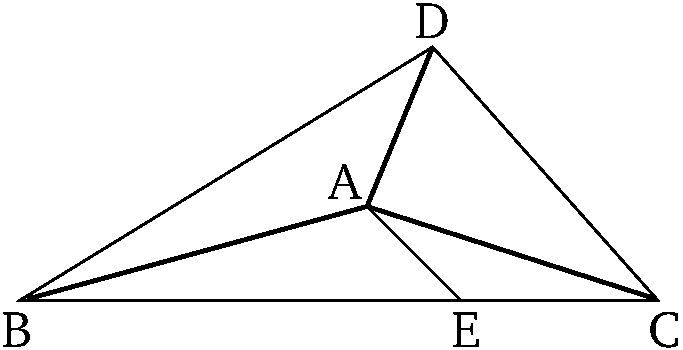
\includegraphics{Book11/fig20e.eps}}

For let the solid angle $A$ be contained by the three plane angles $BAC$, $CAD$, and $DAB$. I say that (the sum of) any two of the angles $BAC$, $CAD$, and $DAB$ is greater than the remaining (one),
(the angles) being taken up in any (possible way).

For if the angles $BAC$, $CAD$, and $DAB$ are equal to one another
then (it is) clear that (the sum of) any two is greater than
the remaining (one). But, if not, let $BAC$ be greater (than $CAD$ or $DAB$). And let (angle) $BAE$, equal to the angle $DAB$,  be constructed in the plane through $BAC$, on the straight-line $AB$,
at the point $A$ on it. And let $AE$ be made equal to $AD$. And $BEC$
being drawn across through point $E$, let it cut the straight-lines $AB$
and $AC$ at points $B$ and $C$ (respectively). And let
$DB$ and $DC$ be joined.

And since $DA$ is equal to $AE$, and $AB$ (is) common, the
two (straight-lines $AD$ and $AB$ are) equal to the two (straight-lines
$EA$ and $AB$, respectively). And angle $DAB$ (is) equal
to angle $BAE$. Thus, the base $DB$ is equal to the base $BE$ [Prop.~1.4]. And since the
(sum of the) two (straight-lines) $BD$ and $DC$ is greater than $BC$
[Prop.~1.20], of which $DB$ was shown
(to be) equal to $BE$, the  remainder $DC$ is thus greater than the
remainder $EC$. And since $DA$ is equal to $AE$, but
$AC$ (is) common, and the base $DC$ is  greater than the base
$EC$, the angle $DAC$ is thus greater than the angle $EAC$
[Prop.~1.25]. And $DAB$
was also shown (to be) equal to $BAE$. Thus, 
(the sum of) $DAB$ and $DAC$ is greater than $BAC$. So,
similarly, we can also show that the remaining  (angles), being taken in pairs, are greater than the remaining (one).

Thus,  if a solid angle is contained by three plane angles
then (the sum of) any two (angles) is greater than the remaining (one), (the angles) being taken up in any (possible way). (Which is) the very thing it
was required to show.}
\end{Parallel}

%%%%
%11.21
%%%%
\pdfbookmark[1]{Proposition 11.21}{pdf11.21}
\begin{Parallel}{}{}
\ParallelLText{
\begin{center}
{\large \ggn{21}.}
\end{center}\vspace*{-7pt}

\gr{<'Απασα στερεὰ γωνία ὑπὸ ἐλασσόνων [>ὴ] τεσσάρων ὀρθῶν
γωνιῶν ἐπιπέδων περιέθεται.}

\epsfysize=1.5in
\centerline{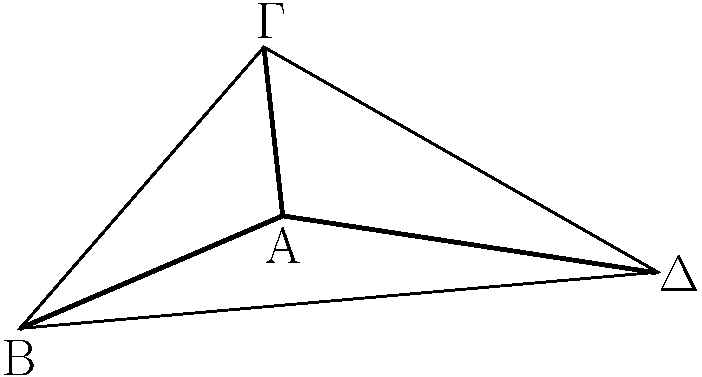
\includegraphics{Book11/fig21g.eps}}

\gr{>'Εστω στερεὰ γωνία ἡ πρὸξ τῶ| Α περιεθομένη ὑπὸ
ἐπιπέδων γωνιῶν τῶν ὑπὸ ΒΑΓ, ΓΑΔ, ΔΑΒ; λέγω, <ότι
αἱ ὑπὸ ΒΑΓ, ΓΑΔ, ΔΑΒ τεσσάρων ὀρθῶν ἐλάσσονέξ εἰσιν.}

\gr{Εἰλήφθω γὰρ ἐφ> ἑκάστηξ τῶν ΑΒ, ΑΓ, ΑΔ τυθόντα σημεῖα
τὰ Β, Γ, Δ, καὶ ἐπεζεύθθωσαν αἱ ΒΓ, ΓΔ, ΔΒ. καὶ ἐπεὶ στερεὰ γωνία
ἡ πρὸξ τῶ| Β ὑπὸ τριῶν γωνιῶν ἐπιπέδων περιέθεται τῶν
ὑπὸ ΓΒΑ, ΑΒΔ, ΓΒΔ, δύο ὁποιαιοῦν τῆξ λοιπῆξ μείζονέξ
εἰσιν; αἱ >άρα ὑπὸ ΓΒΑ, ΑΒΔ τῆξ ὑπὸ ΓΒΔ μείζονέξ
εἰσιν.
διὰ τὰ α\kern -.7pt  ὐτὰ δὴ καὶ αἱ μὲν ὑπὸ ΒΓΑ, ΑΓΔ τῆξ ὑπὸ ΒΓΔ
μείζονέξ εἰσιν, αἱ  δὲ ὑπὸ ΓΔΑ, ΑΔΒ τῆξ ὑπὸ ΓΔΒ μείζονέξ
εἰσιν; αἱ <ὲχ >άρα γωνίαι αἱ ὑπὸ ΓΒΑ, ΑΒΔ, ΒΓΑ, ΑΓΔ, ΓΔΑ, ΑΔΒ τριῶν τῶν ὑπὸ ΓΒΔ, ΒΓΑ, ΓΔΒ μείζονέξ εἰσιν. ἀλλὰ αἱ
τρεῖξ αἱ ὑπὸ ΓΒΔ, ΒΔΓ, ΒΓΔ δυσὶν ὀρθαῖξ >ίσαι εἰσίν;
αἱ <ὲχ >άρα αἱ ὑπὸ ΓΒΑ, ΑΒΔ, ΒΓΑ, ΑΓΔ, ΓΔΑ, ΑΔΒ δύο
ὀρθῶν μείζονέξ εἰσιν. καὶ ἐπεὶ ἑκάστου τῶν ΑΒΓ, ΑΓΔ, ΑΔΒ
τριγώνων αἱ τρεῖξ γωνίαι δυσὶν ὀρθαῖξ >ίσαι εἰσίν, αἱ >άρα
τῶν τριῶν τριγώνων ἐννέα γωνίαι αἱ ὑπὸ ΓΒΑ, ΑΓΒ, ΒΑΓ, ΑΓΔ,
ΓΔΑ, ΓΑΔ, ΑΔΒ, ΔΒΑ, ΒΑΔ 	<ὲχ ὀρθαῖξ >ίσαι
εἰσίν, <ῶν αἱ ὑπὸ ΑΒΓ, ΒΓΑ, ΑΓΔ, ΓΔΑ, ΑΔΒ,
ΔΒΑ <ὲχ γωνίαι δύο ὀρθῶν εἰσι μείζονεξ; λοιπαὶ >άρα
αἱ ὑπὸ ΒΑΓ, ΓΑΔ, ΔΑΒ τρεῖξ [γωνίαι] περιέθουσαι τὴν στερεὰν
γωνίαν τεσσάρων ὀρθῶν ἐλάσσονέξ εἰσιν.}

\gr{<'Απασα >άρα στερεὰ γωνία ὑπὸ ἐλασσόνων [>ή] τεσσάρων ὀρθῶν
γωνιῶν ἐπιπέδων περιέθεται; <όπερ >έδει δεῖχαι.}}

\ParallelRText{
\begin{center}
{\large Proposition 21}
\end{center}

Any solid angle is contained by plane angles (whose sum is) less [than]
four  right-angles.$^\dag$

\epsfysize=1.5in
\centerline{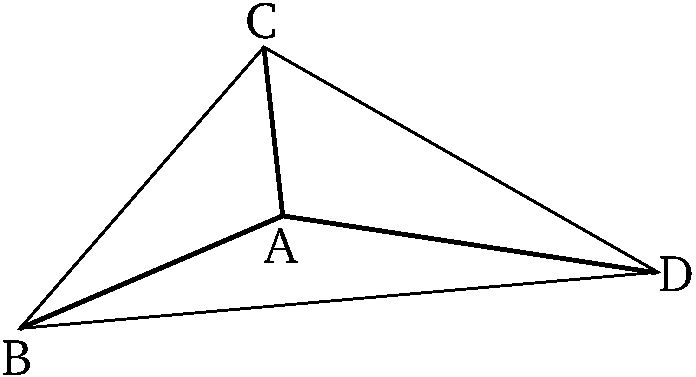
\includegraphics{Book11/fig21e.eps}}

Let the solid angle $A$ be contained by the plane angles $BAC$,
$CAD$, and $DAB$. I say that (the sum of) $BAC$, $CAD$, and $DAB$
is less than four right-angles.

For let the random points $B$, $C$, and $D$ be taken on each of (the straight-lines)
 $AB$, $AC$, and $AD$ (respectively). And let $BC$, $CD$, and $DB$ be joined.  And since the solid angle at $B$ is contained
by the three plane angles $CBA$, $ABD$, and $CBD$, (the sum of) any two
is greater than the remaining (one) [Prop.~11.20].
Thus, (the sum of) $CBA$ and $ABD$ is greater than $CBD$. So, for
the same (reasons), (the sum of) $BCA$ and $ACD$ is also greater than
$BCD$, and (the sum of) $CDA$ and $ADB$ is greater than $CDB$.
Thus, the (sum of the) six angles $CBA$, $ABD$, $BCA$, $ACD$, $CDA$,
and $ADB$ is greater than the (sum of the) three (angles) $CBD$, $BCD$,
and $CDB$. But, the (sum of the) three (angles) $CBD$, $BDC$, and
$BCD$ is equal to two right-angles [Prop.~1.32].
Thus, the (sum of the) six angles $CBA$, $ABD$, $BCA$, $ACD$, $CDA$,
and $ADB$ is greater than two right-angles.
And since the (sum of the) three angles of each of the triangles
$ABC$, $ACD$, and $ADB$ is equal to two right-angles, the (sum of the)
nine angles $CBA$, $ACB$, $BAC$, $ACD$, $CDA$, $CAD$, $ADB$,
$DBA$, and $BAD$ of the three triangles is equal to six right-angles,
of which the (sum of the) six angles $ABC$, $BCA$, $ACD$, $CDA$,
$ADB$, and $DBA$ is greater than two right-angles. Thus, the (sum of the)
remaining three [angles] $BAC$, $CAD$, and $DAB$, containing the
solid angle, is less than four right-angles.

Thus, any solid angle is contained by plane angles (whose sum is) less [than]
four  right-angles. (Which is) the very thing it was required to show.}
\end{Parallel}
{\footnotesize\noindent$^\dag$ This proposition is only proved for the case of a solid angle contained by three plane angles. However, the generalization to
a solid angle contained by more than three plane angles is straightforward.}

%%%%
%11.22
%%%%
\pdfbookmark[1]{Proposition 11.22}{pdf11.22}
\begin{Parallel}{}{}
\ParallelLText{
\begin{center}
{\large \ggn{22}.}
\end{center}\vspace*{-7pt}

\gr{Ἐὰν <ῶσι τρεῖξ γωνίαι ἐπίπεδοι, <ῶν αἱ δύο τῆξ λοιπῆξ μείζονέξ εἰσι πάντῃ μεταλαμβανόμεναι, περιέθωσι δὲ α\kern -.7pt  ὐτὰξ
>ίσαι εὐθεῖαι, δυνατόν ἐστιν ἐκ τῶν ἐπιζευγνυουσῶν τὰξ
>ίσαξ εὐθείαξ τρίγωνον συστήσασθαι.}\\~\\

\epsfysize=.9in
\centerline{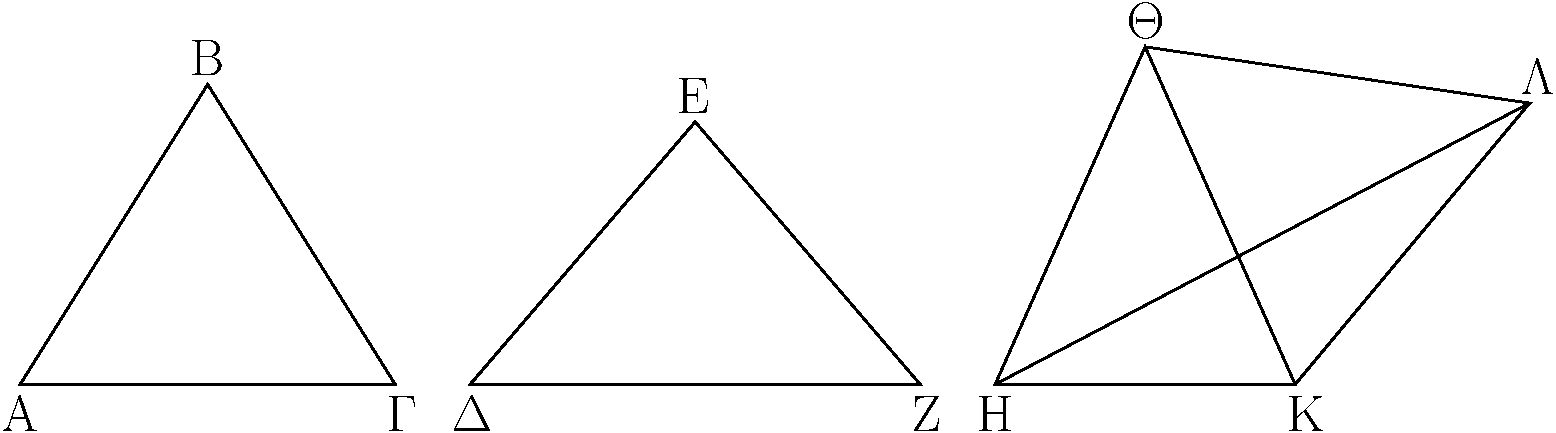
\includegraphics{Book11/fig22g.eps}}

\gr{>'Εστωσαν τρεῖξ γωνίαι ἐπίπεδοι αἱ ὑπὸ ΑΒΓ, ΔΕΖ, ΗJΚ, <ῶν
αἱ δύο τῆξ λοιπῆξ μείζονέξ εἰσι πάντῃ μεταλαμβανόμεναι, αἱ
μὲν ὑπὸ ΑΒΓ, ΔΕΖ τῆξ ὑπὸ ΗJΚ, αἱ δὲ ὑπὸ ΔΕΖ, ΗJΚ
τῆξ ὑπὸ ΑΒΓ, καὶ >έτι αἱ ὑπὸ ΗJΚ, ΑΒΓ τῆξ ὑπὸ ΔΕΖ,
καὶ >έστωσαν >ίσαι αἱ ΑΒ, ΒΓ, ΔΕ, ΕΖ, ΗJ, JΚ εὐθεῖαι,
καὶ ἐπεζεύθθωσαν αἱ ΑΓ, ΔΖ, ΗΚ; λέγω, <ότι δυνατόν ἐστιν
ἐκ τῶν >ίσων ταῖξ ΑΓ, ΔΖ, ΗΚ τρίγωνον συστήσασθαι, τουτέστιν
<ότι τῶν ΑΓ, ΔΖ, ΗΚ δύο ὁποιαιοῦν τῆξ λοιπῆξ μείζονέξ
εἰσιν.}

\gr{Εἰ μὲν ο>ῦν αἱ ὑπὸ ΑΒΓ, ΔΕΖ, ΗJΚ γωνίαι >ίσαι ἀλλήλαιξ
εἰσίν, φανερόν, <ότι καὶ τῶν ΑΓ, ΔΖ, ΗΚ >ίσων γινομένων δυνατόν
ἐστιν ἐκ τῶν >ίσων ταῖξ ΑΓ, ΔΖ, ΗΚ τρίγωνον συστήσασθαι.
εἰ δὲ ο>ύ,  >έστωσαν >άνισοι, καὶ συνεστάτω πρὸξ τῆ| JΚ
εὐθείᾳ καὶ τῶ| πρὸξ α\kern -.7pt  ὐτῆ| σημείῳ τῶ| J τῆ| ὑπὸ ΑΒΓ
γωνίᾳ >ίση ἡ ὑπὸ ΚJΛ; καὶ κείσθω μιᾶ| τῶν ΑΒ, ΒΓ, ΔΕ, ΕΖ,
ΗJ, JΚ >ίση ἡ JΛ, καὶ ἐπεζεύθθωσαν αἱ ΚΛ, ΗΛ. καὶ ἐπεὶ
δύο αἱ ΑΒ, ΒΓ δυσὶ ταῖξ ΚJ, JΛ
>ίσαι εἰσίν, καὶ γωνία ἡ πρὸξ τῶ| Β γωνίᾳ τῆ| ὑπὸ ΚJΛ >ίση,
βάσιξ >άρα ἡ ΑΓ βάσει τῆ| ΚΛ >ίση. καὶ ἐπεὶ αἱ ὑπὸ ΑΒΓ,
ΗJΚ τῆξ ὑπὸ ΔΕΖ μείζονέξ εἰσιν, >ίση δὲ ἡ ὑπὸ ΑΒΓ
τῆ| ὑπὸ ΚJΛ, ἡ >άρα ὑπὸ ΗJΛ τῆξ ὑπὸ ΔΕΖ μείζων ἐστίν. καὶ
ἐπεὶ δύο αἱ ΗJ, JΛ δύο ταῖξ ΔΕ, ΕΖ >ίσαι εἰσίν, καὶ γωνία
ἡ ὑπὸ ΗJΛ γωνίαξ τῆξ ὑπὸ ΔΕΖ μείζων, βάσιξ >άρα
ἡ ΗΛ βάσεωξ τῆξ ΔΖ μείζων ἐστίν. ἀλλὰ αἱ ΗΚ, ΚΛ
τῆξ ΗΛ μείζονέξ εἰσιν. πολλῶ| >άρα αἱ ΗΚ, ΚΛ τῆξ
ΔΖ μείζονέξ εἰσιν. >ίση δὲ ἡ ΚΛ τῆ| ΑΓ; αἱ ΑΓ, ΗΚ >άρα
τῆξ λοιπῆξ τῆξ ΔΖ μείζονέξ εἰσιν. ὁμοίωξ δὴ δείχομεν, 
<ότι καὶ αἱ μὲν ΑΓ, ΔΖ τῆξ ΗΚ μείζονέξ εἰσιν, καὶ >έτι
αἱ ΔΖ, ΗΚ τῆξ ΑΓ μείζονέξ εἰσιν. δυνατὸν >άρα ἐστὶν ἐκ
τῶν >ίσων ταῖξ ΑΓ, ΔΖ, ΗΚ τρίγωνον συστήσασθαι; <όπερ >έδει
δεῖχαι.}}

\ParallelRText{
\begin{center}
{\large Proposition 22}
\end{center}

If there are three plane angles, of which (the sum of any)
two is greater than the remaining (one), (the angles) being taken up in
any (possible way), and if equal straight-lines contain them, then it is
possible to construct a triangle from (the straight-lines created by) joining the
(ends of the) equal straight-lines.

\epsfysize=0.9in
\centerline{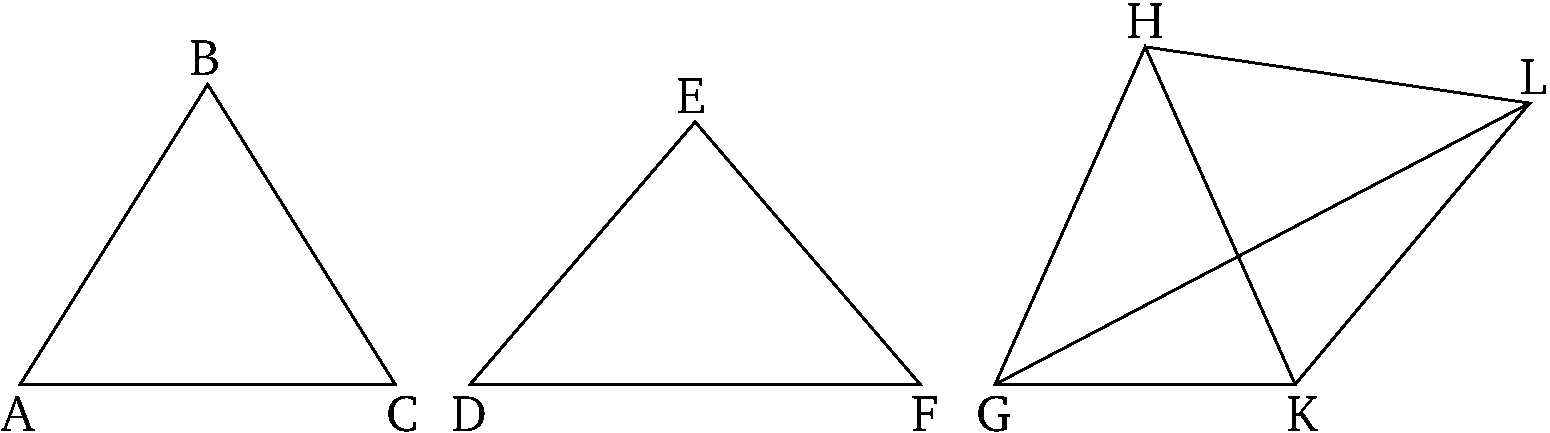
\includegraphics{Book11/fig22e.eps}}

Let $ABC$, $DEF$, and $GHK$ be three plane angles, of which the sum of any)
two is greater than the remaining (one), (the angles) being taken up in
any (possible way)---(that is), $ABC$ and $DEF$ (greater) than $GHK$,
$DEF$ and $GHK$ (greater) than $ABC$, and, further, $GHK$
and $ABC$ (greater) than $DEF$. And let $AB$, $BC$, $DE$, $EF$,
$GH$, and $HK$ be equal straight-lines. And let $AC$, $DF$, and
$GK$ be joined. I say that that it is possible to construct a
triangle out of (straight-lines) equal to $AC$, $DF$, and $GK$---that is to say, that (the sum of) any two of $AC$, $DF$, and $GK$ is greater than
the remaining (one).

Now, if the angles $ABC$, $DEF$, and $GHK$ are equal to one another then
(it is)  clear that, (with) $AC$, $DF$, and $GK$ also becoming equal, it is
possible to construct a triangle from (straight-lines) equal to
$AC$, $DF$, and $GK$. And if not, let them be unequal, and let $KHL$,
equal to angle $ABC$, be constructed on the straight-line
$HK$, at the point $H$ on it. And let $HL$ be made equal to one
of $AB$, $BC$, $DE$, $EF$, $GH$, and $HK$. And let $KL$
and $GL$ be joined. And since the two (straight-lines) $AB$ and
$BC$ are equal to the two (straight-lines) $KH$ and $HL$ (respectively), 
and the angle at $B$ (is) equal to $KHL$, the base $AC$ is thus equal to the
base $KL$ [Prop.~1.4]. And since (the sum of)
$ABC$ and $GHK$ is greater than $DEF$, and $ABC$
equal to $KHL$,  $GHL$ is thus greater than $DEF$. And since the
two (straight-lines) $GH$ and $HL$ are equal to the two (straight-lines)
$DE$ and $EF$ (respectively), and angle $GHL$ (is) greater than $DEF$, the base $GL$ is thus greater than the base $DF$ [Prop.~1.24]. 
But, (the sum of) $GK$ and $KL$ is greater than $GL$ [Prop.~1.20]. Thus, (the sum of) $GK$ and $KL$
is much greater than $DF$.  And $KL$ (is) equal to $AC$. Thus, (the sum of)
$AC$ and $GK$ is greater than the remaining (straight-line) $DF$.
So, similarly, we can show that (the sum of) $AC$ and $DF$
is greater than $GK$, and, further, that (the sum of) $DF$ and $GK$
is greater than $AC$. Thus, it is possible to construct a triangle from
(straight-lines) equal to $AC$, $DF$, and $GK$. (Which is) the very
thing it was required to show.}
\end{Parallel}

%%%%
%11.23
%%%%
\pdfbookmark[1]{Proposition 11.23}{pdf11.23}
\begin{Parallel}{}{}
\ParallelLText{
\begin{center}
{\large\ggn{23}.}
\end{center}\vspace*{-7pt}

\gr{Ἐκ τριῶν γωνιῶν ἐπιπέδων, <ῶν αἱ δύο τῆξ λοιπῆξ
μείζονέξ εἰσι πάντῃ μεταλαμβανόμεναι, στερεὰν γωνίαν συστήσασθαι;
δεῖ δὴ τὰξ τρεῖξ τεσσάρων ὀρθῶν ἐλάσσ\-οναξ ε>ῖναι.}\\~\\

\epsfysize=1.1in
\centerline{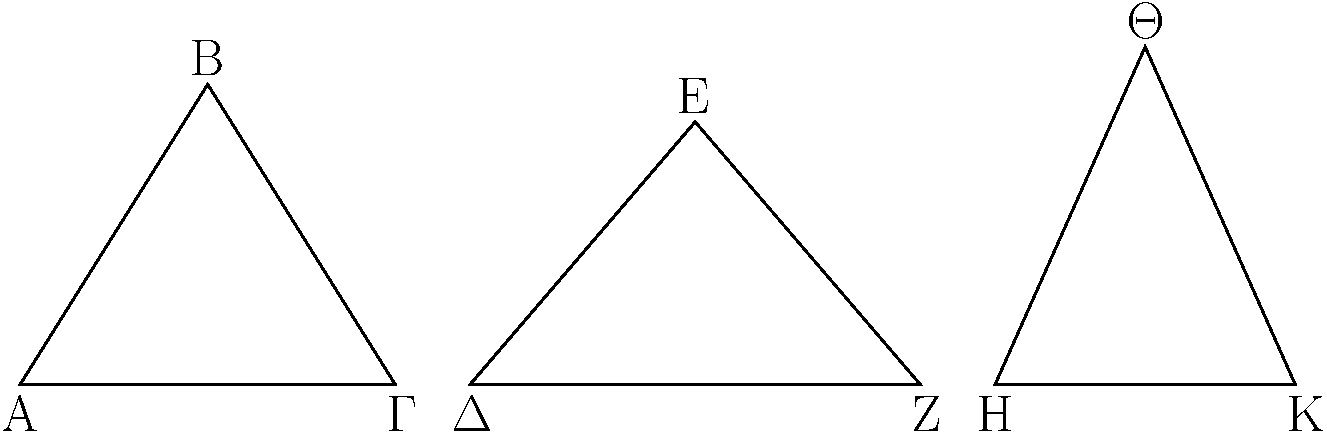
\includegraphics{Book11/fig23g.eps}}

\gr{>'Εστωσαν αἱ δοθεῖσαι τρεῖξ γωνίαι ἐπίπεδοι αἱ ὑπὸ ΑΒΓ, ΔΕΖ,
ΗJΚ, <ῶν αἱ δύο τῆξ λοιπῆξ μείζονεξ >έστωσαν πάντῃ μεταλαμβανόμεναι, >έτι δὲ αἱ τρεῖξ τεσσάρων ὀρθῶν ἐλάσσονεξ;
δεῖ
 δὴ ἐκ τῶν >ίσων ταῖξ ὑπὸ ΑΒΓ, ΔΕΖ,
ΗJΚ στερεὰν γωνίαν συστήσασθαι.}

\gr{Ἀπειλήφθωσαν >ίσαι αἱ ΑΒ, ΒΓ, ΔΕ, ΕΖ, ΗJ, JΚ, καὶ
ἐπεζεύθθωσαν αἱ ΑΓ, ΔΖ, ΗΚ; δυνατὸν >άρα ἐστὶν ἐκ τῶν
>ίσων ταῖξ ΑΓ, ΔΖ, ΗΚ τρίγωνον συστήσασθαι. συνεστάτω τὸ ΛΜΝ,
<ώστε >ίσην ε>ῖναι τὴν μὲν ΑΓ τῆ| ΛΜ, τὴν δὲ ΔΖ τῆ| ΜΝ,
καὶ >έτι τὴν ΗΚ τῆ| ΝΛ, καὶ περιγεγράφθω περὶ τὸ ΛΜΝ
τρίγωνον κύκλοξ ὁ ΛΜΝ, καὶ εἰλήφθω α\kern -.7pt  ὐτοῦ τὸ κέντρον
καὶ >έστω τὸ Χ, καὶ ἐπεζεύθθωσαν αἱ ΛΧ, ΜΧ, ΝΧ;}\\~\\~\\

\epsfysize=2.in
\centerline{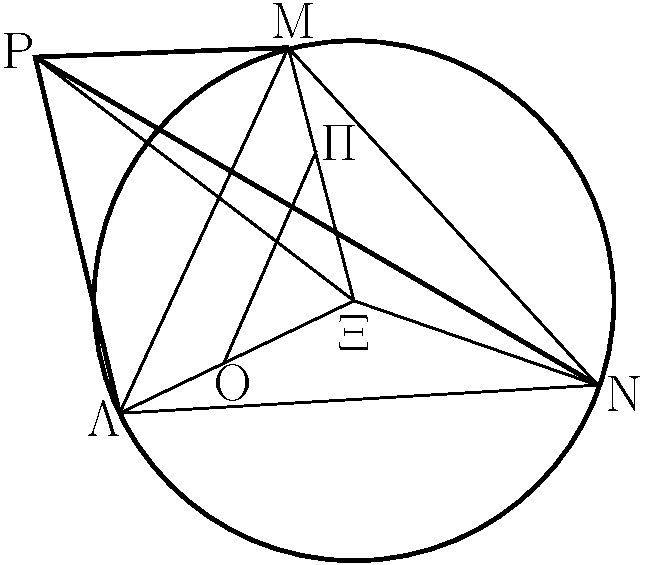
\includegraphics{Book11/fig23ag.eps}}

\gr{ Λέγω,
<ότι ἡ ΑΒ μείζων ἐστὶ τῆξ ΛΧ. εἰ γὰρ μ\kern -.7pt  ή, >ήτοι >ίση
ἐστὶν ἡ ΑΒ τῆ| ΛΧ >ὴ ἐλάττων. >έστω πρότερον >ίση. καὶ
ἐπεὶ >ίση ἐστὶν ἡ ΑΒ τῆ| ΛΧ, ἀλλὰ ἡ μὲν ΑΒ τῆ| ΒΓ ἐστιν
>ίση, ἡ δὲ ΧΛ τῆ| ΧΜ, δύο δὴ αἱ ΑΒ, ΒΓ δύο ταῖξ ΛΧ, ΧΜ
>ίσαι εἰσὶν ἑκατέρα ἑκατέρᾳ; καὶ βάσιξ ἡ ΑΓ βάσει τῆ| ΛΜ ὑπόκειται >ίση; γωνία >άρα ἡ ὑπὸ ΑΒΓ γωνίᾳ τῆ| ὑπὸ
ΛΧΜ ἐστιν >ίση. διὰ τὰ α\kern -.7pt  ὐτὰ δὴ καὶ ἡ μὲν ὑπὸ ΔΕΖ
τῆ| ὑπὸ ΜΧΝ ἐστιν >ίση, καὶ >έτι ἡ ὑπὸ ΗJΚ τῆ| ὑπὸ
ΝΧΛ; αἱ >άρα τρεῖξ αἱ ὑπὸ ΑΒΓ, ΔΕΖ, ΗJΚ γωνίαι τρισὶ
ταῖξ ὑπὸ ΛΧΜ, ΜΧΝ, ΝΧΛ εἰσιν >ίσαι. ἀλλὰ αἱ τρεῖξ αἱ
ὑπὸ ΛΧΜ, ΜΧΝ, ΝΧΛ τέτταρσιν ὀρθαῖξ εἰσιν >ίσαι;
καὶ αἱ τρεῖξ >άρα αἱ ὑπὸ ΑΒΓ, ΔΕΖ, ΗJΚ τέτταρσιν ὀρθαῖξ
>ίσαι εἰσίν. ὑπόκεινται δὲ καὶ τεσσάρων ὀρθῶν ἐλάσσονεξ;
<όπερ >άτοπον. οὐκ >άρα ἡ ΑΒ τῆ| ΛΧ >ίση ἐστίν. λέγω δή,
<ότι οὑδὲ ἐλάττων ἐστὶν ἡ ΑΒ τῆξ ΛΧ. εἰ γὰρ δυνατόν,
>έστω; καὶ κείσθω τῆ| μὲν ΑΒ >ίση ἡ ΧΟ, τῆ| δὲ ΒΓ >ίση
ἡ ΧΠ, καὶ ἐπεζεύθθω ἡ ΟΠ. καὶ ἐπεὶ >ίση ἐστὶν ἡ ΑΒ
τῆ| ΒΓ, >ίση ἐστὶ καὶ ἡ ΧΟ τῆ| ΧΠ; <ώστε καὶ λοιπὴ ἡ ΛΟ
τῆ| ΠΜ ἐστιν >ίση. παράλληλοξ >άρα ἐστὶν ἡ ΛΜ τῆ| ΟΠ, καὶ
ἰσογώνιον τὸ ΛΜΧ τῶ| ΟΠΧ; >έστιν >άρα ὡξ ἡ ΧΛ
πρὸξ ΛΜ, ο<ύτωξ ἡ ΧΟ πρὸξ ΟΠ; ἐναλλὰχ ὡξ ἡ ΛΧ πρὸξ
ΧΟ, ο<ύτωξ ἡ ΛΜ πρὸξ ΟΠ. μείζων δὲ ἡ ΛΧ τῆξ ΧΟ; μείζων
>άρα καὶ ἡ ΛΜ τῆξ ΟΠ. ἀλλὰ ἡ ΛΜ κεῖται τῆ| ΑΓ >ίση; καὶ
ἡ ΑΓ >άρα τῆξ ΟΠ μείζων ἐστίν. ἐπεὶ ο>ῦν δύο αἱ ΑΒ, ΒΓ
δυσὶ ταῖξ ΟΧ, ΧΠ >ίσαι εἰσίν, καὶ βάσιξ ἡ ΑΓ βάσεωξ τῆξ ΟΠ
μείζων ἐστίν, γωνία >άρα ἡ ὑπὸ ΑΒΓ γωνίαξ τῆξ ὑπὸ
ΟΧΠ μεῖζων ἐστίν. ὁμοίωξ δὴ δείχομεν, <ότι καὶ ἡ μὲν
ὑπὸ ΔΕΖ τῆξ ὑπὸ ΜΧΝ μείζων ἐστίν,\, ἡ δὲ ὑπὸ
ΗJΚ τῆξ ὑπὸ ΝΧΛ. αἱ >άρα τρεῖξ γωνίαι αἱ ὑπὸ ΑΒΓ, ΔΕΖ, ΗJΚ
τριῶν τῶν ὑπὸ ΛΧΜ, ΜΧΝ, ΝΧΛ μείζονέξ εἰσιν. ἀλλὰ αἱ ὑπὸ
ΑΒΓ, ΔΕΖ, ΗJΚ τεσσάρων ὀρθῶν ἐλάσσονεξ ὑπόκεινται; πολλῶ|
>άρα αἱ ὑπὸ ΛΧΜ, ΜΧΝ, ΝΧΛ τεσσάρων ὀρθῶν ἐλάσσονέξ εἰσιν.
ἀλλὰ καὶ >ίσαι; <όπερ ἐστὶν >άτοπον. οὐκ >άρα ἡ ΑΒ ἐλάσσων
ἐστὶ τῆξ ΛΧ. ἐδείθθη δέ, <ότι οὐδὲ >ίση; μείζων >άρα ἡ ΑΒ
τῆξ ΛΧ.}

\gr{Ἀνεστάτω δὴ ἀπὸ τοῦ Χ σημείου τῶ| τοῦ ΛΜΝ κύκλου
ἐπιπέδῳ πρὸξ ὀρθὰξ ἡ ΧΡ, καὶ <ῶ| μεῖζόν ἐστι τὸ ἀπὸ τῆξ
ΑΒ τετράγωνον τοῦ ἀπὸ τῆξ ΛΧ, ἐκείνῳ >ίσον >έστω τὸ
ἀπὸ τῆξ ΧΡ, καὶ ἐπεζεύθθωσαν αἱ ΡΛ, ΡΜ, ΡΝ.}

\gr{Καὶ ἐπεὶ ἡ ΡΧ ὀρθὴ ἐστι πρὸξ τὸ τοῦ ΛΜΝ κύκλου
ἐπίπεδον, καὶ πρὸξ ἑκάστην >άρα τῶν ΛΧ, ΜΧ, ΝΧ
ὀρθή ἐστιν ἡ ΡΧ.
 καὶ ἐπεὶ >ίση
ἐστὶν ἡ ΛΧ τῆ| ΧΜ, κοινὴ δὲ καὶ πρὸξ ὀρθὰξ ἡ ΧΡ, βάσιξ >άρα
ἡ ΡΛ βάσει τὴ| ΡΜ ἐστιν >ίση. διὰ τὰ α\kern -.7pt  ὐτὰ δὴ καὶ ἡ ΡΝ
ἑκατέρᾳ τῶν ΡΛ, ΡΜ ἐστιν >ίση; αἱ τρεῖξ >άρα αἱ ΡΛ,
ΡΜ, ΡΝ >ίσαι ἀλλήλαιξ εἰσίν. καὶ ἐπεὶ <ῶ| μεῖζόν
ἐστι τὸ ἀπὸ τῆξ ΑΒ τοῦ ἀπὸ τῆξ ΛΧ, ἐκείνῳ
>ίσον ὑπόκειται τὸ ἀπὸ τῆξ ΧΡ, τὸ >άρα ἀπὸ τῆξ ΑΒ >ίσον
ἐστὶ τοῖξ ἀπὸ τῶν ΛΧ, ΧΡ.  τοῖξ δὲ ἀπὸ τῶν ΛΧ, ΧΡ
>ίσον ἐστὶ τὸ ἀπὸ τῆξ ΛΡ; ὀρθὴ γὰρ ἡ ὑπὸ ΛΧΡ;
τὸ >άρα ἀπὸ τῆξ ΑΒ >ίσον ἐστὶ τῶ| ἀπὸ τῆξ ΡΛ;
>ίση >άρα ἡ ΑΒ τῆ| ΡΛ. ἀλλὰ τῆ| μὲν ΑΒ >ίση ἐστὶν ἑκάστη
τῶν ΒΓ, ΔΕ, ΕΖ, ΗJ, JΚ, τῆ| δὲ ΡΛ >ίση ἑκατέρα τῶν
ΡΜ, ΡΝ;  ἑκάστη >άρα τῶν ΑΒ, ΒΓ, ΔΕ, ΕΖ, ΗJ, JΚ 
ἑκάστῃ τῶν ΡΛ, ΡΜ, ΡΝ >ίση ἐστίν. καὶ ἐπεὶ δύο
αἱ ΛΡ, ΡΜ δυσὶ ταῖξ ΑΒ, ΒΓ >ίσαι εἰσίν, καὶ βάσιξ ἡ ΛΜ
βάσει τῆ| ΑΓ ὑπόκειται >ίση, γωνία >άρα ἡ ὑπὸ ΛΡΜ
γωνίᾳ τῆ| ὑπὸ ΑΒΓ ἐστιν >ίση. διὰ τὰ α\kern -.7pt  ὐτὰ δὴ καὶ ἡ μὲν ὑπὸ
ΜΡΝ τῆ| ὑπὸ ΔΕΖ ἐστιν >ίση, ἡ δὲ ὑπὸ ΛΡΝ τῆ| ὑπὸ
ΗJΚ.}

\gr{Ἐκ τριῶν >άρα γωνιῶν ἐπιπέδων τῶν ὑπὸ ΛΡΜ, ΜΡΝ, ΛΡΝ,
α<ί εἰσιν >ίσαι τρισὶ ταῖξ δοθείσαιξ ταῖξ ὑπὸ ΑΒΓ, ΔΕΖ, ΗJΚ,
στερεὰ γωνία συνέσταται ἡ πρὸξ τῶ| Ρ περιεθομένη ὑπὸ τῶν
ΛΡΜ, ΜΡΝ, ΛΡΝ γωνιῶν; <όπερ >έδει ποιῆσαι.}}

\ParallelRText{
\begin{center}
{\large Proposition 23}
\end{center}

To construct a solid angle from three (given)
plane angles,  (the sum of) two of which is greater than the remaining (one, the
angles) being taken up in any (possible way). So, it is necessary for the (sum of the) three (angles) to be less than four right-angles [Prop.~11.21].

\epsfysize=1.1in
\centerline{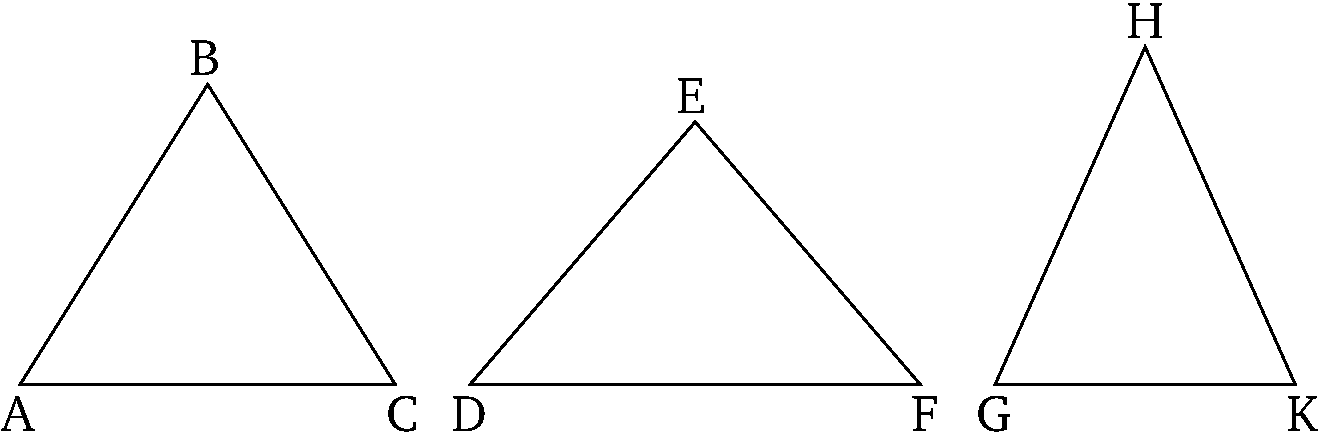
\includegraphics{Book11/fig23e.eps}}

Let $ABC$, $DEF$, and $GHK$ be the three given plane angles, of which let
(the sum of) two be greater than the remaining (one, the angles) being taken
up in any (possible way), and, further, (let) the (sum of the) three (be) less than
four right-angles. So, it is necessary to construct a solid angle from
(plane angles) equal to $ABC$, $DEF$, and $GHK$.

Let $AB$, $BC$, $DE$, $EF$, $GH$, and $HK$ be cut off (so as to be)
equal (to one another). And let $AC$, $DF$, and $GK$ be joined.
It is, thus, possible to construct a triangle from (straight-lines) equal to
$AC$, $DF$, and $GK$ [Prop.~11.22]. Let
(such a triangle), $LMN$, have be constructed, such that $AC$ is equal to
$LM$, $DF$ to $MN$, and, further, $GK$ to $NL$. And let the circle
$LMN$ be circumscribed about triangle $LMN$ [Prop.~4.5]. And let its center be found, and let it be (at) $O$.
And let $LO$, $MO$, and $NO$ be joined.

\epsfysize=2.in
\centerline{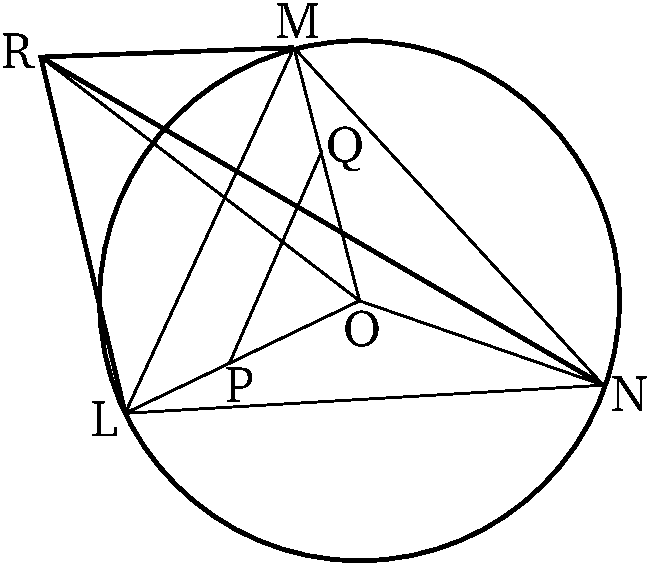
\includegraphics{Book11/fig23ae.eps}}

 I say that $AB$ is greater
than $LO$. For, if not, $AB$ is either equal to, or less than, $LO$.
Let it, first of all, be equal. And since $AB$ is equal to $LO$, but $AB$
is equal to $BC$, and $OL$ to $OM$, so the two (straight-lines)
$AB$ and $BC$ are equal to the two (straight-lines) $LO$ and $OM$, respectively. And the base $AC$ was assumed (to be) equal to the base
$LM$. Thus, angle $ABC$ is equal to angle $LOM$ [Prop.~1.8]. So, for the same (reasons), $DEF$ is also equal to $MON$,
and, further, $GHK$ to $NOL$. Thus, the three angles $ABC$, $DEF$,
and $GHK$ are equal to the three angles $LOM$, $MON$, and $NOL$,
respectively. But, the (sum of the) three angles $LOM$, $MON$,
and $NOL$ is equal to four right-angles. 
Thus, the (sum of the) three angles $ABC$, $DEF$, and $GHK$ is
also equal to four right-angles.
And it was also assumed (to be)
less than four right-angles. The very thing (is) absurd. Thus, $AB$
is not equal to $LO$. So, I say that $AB$ is not less than $LO$ either.
For, if possible, let it be (less). And let $OP$ be made equal to $AB$, and
$OQ$ equal to $BC$, and let $PQ$ be joined. And since $AB$ is equal
to $BC$, $OP$ is also equal to $OQ$. Hence, the remainder $LP$ is also
equal to (the remainder) $QM$. $LM$ is thus parallel to $PQ$ [Prop.~6.2], and (triangle) $LMO$ (is) equiangular with (triangle) $PQO$
[Prop.~1.29]. 
Thus, as $OL$ is to $LM$, so $OP$ (is) to $PQ$ [Prop.~6.4]. Alternately, as $LO$ (is) to $OP$, so $LM$ (is) to $PQ$
[Prop.~5.16]. And $LO$ (is) greater than $OP$. 
Thus, $LM$ (is) also greater than $PQ$ [Prop.~5.14]. 
But $LM$ was made equal to $AC$. Thus, $AC$ is also greater than $PQ$. Therefore, since the two
(straight-lines) $AB$ and $BC$ are equal
to the two (straight-lines) $PO$ and $OQ$ (respectively), and the base $AC$ is greater
than the base $PQ$, the angle $ABC$ is thus greater than the
angle $POQ$ [Prop.~1.25]. So, similarly,
we can show that $DEF$ is also greater than $MON$, and $GHK$ than
$NOL$. Thus, the (sum of the) three angles $ABC$, $DEF$, and
$GHK$ is greater than the (sum of the) three angles $LOM$, $MON$, and
$NOL$. But, (the sum of) $ABC$, $DEF$, and $GHK$ was assumed (to be)
less than four right-angles. Thus, (the sum of) $LOM$, $MON$, and
$NOL$ is much less than four right-angles. But, (it is) also equal (to four right-angles). The very thing is absurd. Thus, $AB$ is not less than $LO$.
And it was shown (to be) not equal either. Thus, $AB$ (is) greater  than
$LO$.

So let $OR$ be set up at point $O$ at right-angles to the plane
of circle $LMN$ [Prop.~11.12]. And let the (square) on $OR$ be equal to that (area) by which the square on $AB$ is greater than the
(square) on $LO$ [Prop.~11.23~lem.]. And let $RL$, $RM$, and $RN$ be joined.

And since $RO$ is at right-angles to the plane of circle $LMN$, $RO$
is thus also at right-angles to each of $LO$, $MO$, and $NO$. And since
$LO$ is equal to $OM$, and $OR$ is common and at right-angles,
the base $RL$ is thus equal to the base $RM$ [Prop.~1.4]. So, for the same (reasons), $RN$ is also equal to
each of $RL$ and $RM$. Thus, the three (straight-lines) $RL$, $RM$,
and $RN$ are equal to one another. And since the (square) on $OR$
was assumed to be equal to that (area) by which the (square) on $AB$
is greater than the (square) on $LO$, the (square) on $AB$ is thus equal
to the (sum of the squares) on $LO$ and $OR$. And the (square) on 
$LR$ is equal to the (sum of the squares) on $LO$ and $OR$. For $LOR$ (is) a right-angle  [Prop.~1.47]. Thus,
the (square) on $AB$ is equal to the (square) on $RL$. Thus, $AB$ (is)
equal to $RL$. But, each of $BC$, $DE$, $EF$, $GH$, and $HK$
is equal to $AB$, and each of $RM$ and $RN$ equal to $RL$. Thus,
each of $AB$, $BC$, $DE$, $EF$, $GH$, and $HK$ is equal to each of
$RL$, $RM$, and $RN$. And since the two (straight-lines)
$LR$ and $RM$ are equal to the two (straight-lines) $AB$ and $BC$ (respectively), and the base $LM$ was assumed (to be) equal to the
base $AC$, the angle $LRM$ is thus equal to the angle $ABC$
[Prop.~1.8]. So, for the same (reasons), $MRN$
is also equal to $DEF$, and $LRN$ to $GHK$.

Thus, the solid angle $R$, contained by the angles $LRM$, $MRN$, and $LRN$,  has been constructed out of the three plane
angles $LRM$, $MRN$, and $LRN$, which are equal to the three
given (plane angles) $ABC$, $DEF$, and $GHK$ (respectively). 
(Which is) the very thing it was required to do.}
\end{Parallel}

\begin{Parallel}{}{}
\ParallelLText{

\epsfysize=1.2in
\centerline{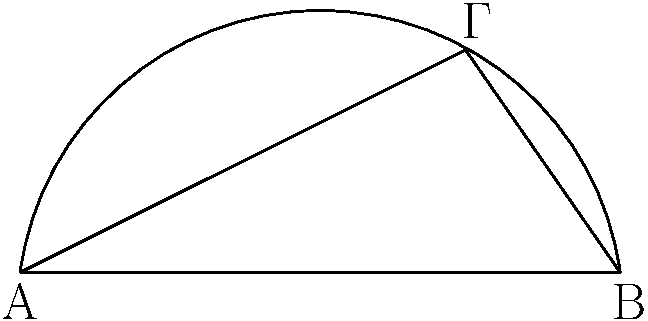
\includegraphics{Book11/fig23bg.eps}}

\begin{center}
{\large \gr{Λῆμμα}.}
\end{center}\vspace*{-7pt}

\gr{<`Ον δὲ τρόπον, <ῶ| μεῖζόν ἐστι τὸ ἀπὸ τῆξ ΑΒ τοῦ ἀπὸ
τῆξ ΛΧ, ἐκείνῳ >ίσον λαβεῖν >έστι τὸ ἀπὸ τῆξ ΧΡ, δείχομεν ο<ύτωξ. ἐκκείσθωσαν αἱ ΑΒ, ΛΧ εὐθεῖαι, καὶ >έστω μείζων
ἡ ΑΒ, καὶ γεγράφθω ἐπ> α\kern -.7pt  ὐτῆξ ἡμικύκλιον τὸ ΑΒΓ, καὶ
εἰξ τὸ ΑΒΓ ἡμικύκλιον ἐνηρμόσθω τῆ| ΛΧ εὐθείᾳ μ\kern -.7pt  ὴ μείζονι
ο>ύσῃ τῆξ ΑΒ διαμέτρου >ίση ἡ ΑΓ, καὶ ἐπεζεύθθω ἡ ΓΒ.
ἐπεὶ ο>ῦν ἐν ἡμικυκλίῳ τῶ| ΑΓΒ γωνία ἐστὶν ἡ ὑπὸ
ΑΓΒ, ὀρθὴ >άρα ἐστὶν ἡ ὑπὸ ΑΓΒ. τὸ >άρα ἀπὸ τῆξ
ΑΒ >ίσον ἐστὶ τοῖξ ἀπὸ τῶν ΑΓ, ΓΒ. <ώστε τὸ ἀπὸ τῆξ
ΑΒ τοῦ ἀπὸ τῆξ ΑΓ μεῖζόν ἐστι τῶ| ἀπὸ τῆξ ΓΒ. >ίση
δὲ ἡ ΑΓ τῆ| ΛΧ. τὸ >άρα ἀπὸ τῆξ ΑΒ τοῦ ἀπὸ τῆξ
ΛΧ μεῖζόν ἐστι τῶ| ἀπὸ τῆξ ΓΒ. ἒαν ο>ῦν τῆ| ΒΓ
>ίσην τὴν ΧΡ ἀπολάβωμεν, >έσται τὸ ἀπὸ τῆξ ΑΒ τοῦ
ἀπὸ τῆξ ΛΧ μεῖζον τῶ| ἀπὸ τῆξ ΧΡ; <όπερ προέκειτο
ποιῆσαι.}}

\ParallelRText{

\epsfysize=1.2in
\centerline{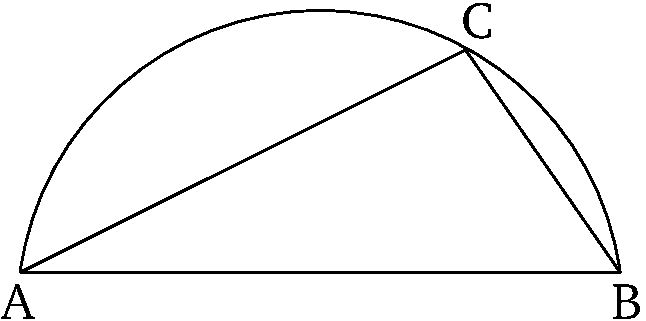
\includegraphics{Book11/fig23be.eps}}

\begin{center}
{\large Lemma}
\end{center}\vspace*{-7pt}

And we can demonstrate, thusly,  in which manner to take the (square) on $OR$ equal to that (area) by which
the (square) on $AB$ is greater than the (square) on $LO$. Let the straight-lines $AB$ and $LO$ be set out, and let $AB$ be greater, and let the semicircle $ABC$ be drawn around it.  And
let $AC$, equal to the  straight-line $LO$, which is not greater than the diameter $AB$,  be inserted into the semicircle $ABC$ [Prop.~4.1]. And let $CB$ be joined. Therefore, since
the angle  $ACB$ is in the semicircle $ACB$, $ACB$ is thus a right-angle
[Prop.~3.31]. Thus, the (square) on $AB$
is  equal to the (sum of the) squares on $AC$ and $CB$ [Prop.~1.47]. Hence, the (square) on $AB$ is greater than the
(square) on $AC$ by the (square) on $CB$. And $AC$ (is) equal to $LO$.
Thus, the (square) on $AB$ is greater than the
(square) on $LO$ by the (square) on $CB$. Therefore, if we take
$OR$ equal to $BC$ then the (square) on $AB$ will be greater than the
(square) on $LO$ by the (square) on $OR$. (Which is) the very thing
it was prescribed to do.}
\end{Parallel}

%%%%
%11.24
%%%%
\pdfbookmark[1]{Proposition 11.24}{pdf11.24}
\begin{Parallel}{}{}
\ParallelLText{
\begin{center}
{\large \ggn{24}.}
\end{center}\vspace*{-7pt}

\gr{Ἐὰν στερεὸν ὑπὸ παραλλήλων ἐπιπέδων περιέθηται, τὰ ἀπεναντίον
α\kern -.7pt  ὐτοῦ ἐπίπεδα >ίσα τε καὶ παραλληλόγραμμά ἐστιν.}

\epsfysize=1.5in
\centerline{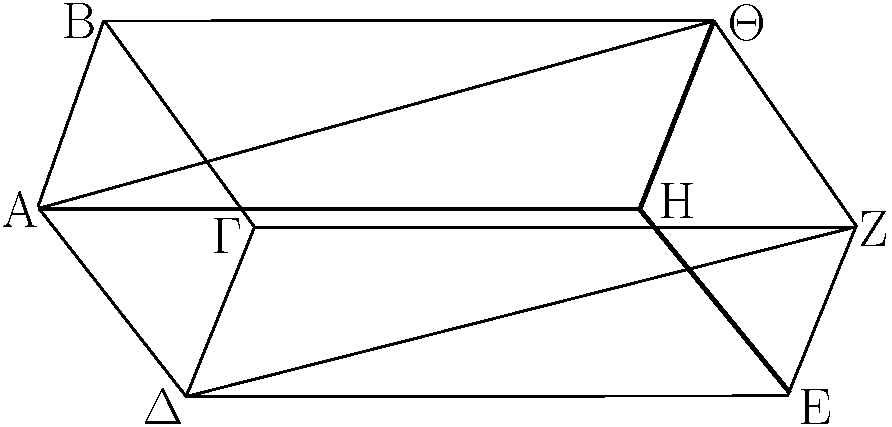
\includegraphics{Book11/fig24g.eps}}

\gr{Στερεὸν γὰρ τὸ ΓΔJΗ ὑπὸ παραλλήλων ἐπιπέδων περιεθέσθω
τῶν ΑΓ, ΗΖ, ΑJ, ΔΖ, ΒΖ, ΑΕ; λέγω, <ότι τὰ ἀπεναντίον α\kern -.7pt  ὐτοῦ
ἐπίπεδα >ίσα τε καὶ παραλληλόγραμμά ἐστιν.}

\gr{Ἐπεὶ γὰρ δύο ἐπίπεδα παράλληλα τὰ ΒΗ, ΓΕ ὑπὸ ἐπιπέδου
τοῦ ΑΓ τέμνεται, αἱ κοιναὶ α\kern -.7pt  ὐτῶν τομαὶ παράλληλοί εἰσιν. παράλληλοξ
>άρα ἐστὶν ἡ ΑΒ τῆ| ΔΓ. πάλιν, ἑπεὶ δύο ἐπίπεδα παράλληλα τὰ ΒΖ,
ΑΕ ὑπὸ ἐπιπέδου τοῦ ΑΓ τέμνεται, αἱ κοιναὶ α\kern -.7pt  ὐτῶν τομαὶ παράλληλοί εἰσιν. παράλληλοξ >άρα ἐστὶν ἡ ΒΓ τῆ| ΑΔ. ἐδείθθη δὲ
καὶ ἡ ΑΒ τῆ| ΔΓ παράλληλοξ; παραλληλόγραμμον >άρα ἐστὶ τὸ ΑΓ.
ὁμοίωξ δὴ δείχομεν, <ότι καὶ <έκαστον τῶν ΔΖ, ΖΗ, ΗΒ, ΒΖ, ΑΕ
παραλληλόγραμμόν ἐστιν.}

\gr{Ἐπεζεύθθωσαν αἱ ΑJ, ΔΖ. καὶ ἐπεὶ παράλληλόξ ἐστιν ἡ μὲν ΑΒ
τῆ| ΔΓ, ἡ δὲ ΒJ τῆ| ΓΖ, δύο δὴ αἱ ΑΒ, ΒJ ἁπτόμεναι ἀλλήλων
παρὰ δύο εὐθείαξ τὰξ ΔΓ, ΓΖ ἁπτομέναξ ἀλλήλων εἰσὶν οὐκ
ἐν τῶ| α\kern -.7pt  ὐτῶ| ἐπιπέδῳ; >ίσαξ >άρα γωνίαξ περιέχουσιν; >ίση
>άρα ἡ ὑπὸ ΑΒJ γωνία τῆ| ὑπὸ ΔΓΖ. καὶ ἐπεὶ δύο αἱ ΑΒ, ΒJ
δυσὶ ταῖξ ΔΓ, ΓΖ >ίσαι εἰσίν, καὶ γωνία ἡ ὑπὸ ΑΒJ
γωνίᾳ τῆ| ὑπὸ ΔΓΖ ἐστιν >ίση, βάσιξ >άρα ἡ ΑJ βάσει
τῆ| ΔΖ ἐστιν >ίση, καὶ τὸ ΑΒJ τρίγωνον τῶ| ΔΓΖ τριγώνῳ >ίσον
ἐστίν. καί ἐστι τοῦ μὲν ΑΒJ διπλάσιον τὸ ΒΗ παραλληλόγραμμον,
τοῦ δὲ ΔΓΖ διπλάσιον τὸ ΓΕ παραλληλόγραμμον; >ίσον >άρα
τὸ ΒΗ παραλληλόγραμμον τῶ| ΓΕ παραλληλογράμμῳ; ὁμοίωξ
δὴ δείχομεν, <ότι καὶ τὸ μὲν ΑΓ τῶ| ΗΖ ἐστιν >ίσον, τὸ δὲ
ΑΕ τῶ| ΒΖ.}

\gr{Ἐὰν >άρα στερεὸν ὑπὸ παραλλήλων ἐπιπέδων περιέθ\-ηται, τὰ ἀπεναντίον
α\kern -.7pt  ὐτοῦ ἐπίπεδα >ίσα τε καὶ παραλληλόγραμμά ἐστιν; <όπερ >έδει
δεῖχαι.}}

\ParallelRText{
\begin{center}
{\large Proposition 24}
\end{center}

If a solid (figure) is contained by (six) parallel planes then its opposite planes
are both equal and parallelogrammic.

\epsfysize=1.5in
\centerline{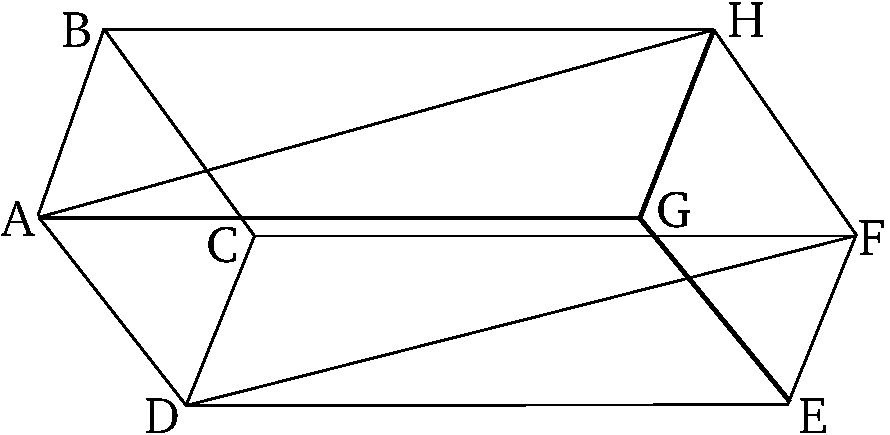
\includegraphics{Book11/fig24e.eps}}

For let the solid (figure) $CDHG$ be contained by the parallel planes
$AC$, $GF$, and $AH$, $DF$, and $BF$, $AE$. I say that its opposite
planes are both equal and parallelogrammic.

For since the two parallel planes $BG$ and $CE$ are cut by the plane
$AC$, their common sections are parallel [Prop.~11.16]. Thus, $AB$ is parallel to $DC$.  Again, since
the two parallel planes $BF$ and $AE$ are cut by the plane
$AC$, their common sections are parallel [Prop.~11.16]. Thus,  $BC$ is parallel to $AD$. And
$AB$ was also shown (to be) parallel to $DC$. Thus, $AC$ is a parallelogram. So, similarly, we can also show that $DF$, $FG$, $GB$,
$BF$, and $AE$ are each parallelograms.

Let $AH$ and $DF$ be joined. And since $AB$ is parallel to
$DC$, and $BH$ to $CF$, so the two (straight-lines) joining one another,
$AB$ and $BH$,
are parallel to the two straight-lines joining one another, $DC$ and
$CF$ (respectively), not (being) in the same plane. Thus, they
will contain equal angles [Prop.~11.10]. Thus,
angle $ABH$ (is) equal to (angle) $DCF$. And since the two (straight-lines)
$AB$ and $BH$ are equal to the two (straight-lines) $DC$ and $CF$ (respectively) [Prop.~1.34], and angle $ABH$ is equal to angle $DCF$, the base
$AH$ is thus equal to the base $DF$, and triangle $ABH$ is equal to
triangle $DCF$ [Prop.~1.4]. And parallelogram
$BG$ is double (triangle) $ABH$, and parallelogram $CE$
double (triangle) $DCF$ [Prop.~1.34]. Thus,
parallelogram $BG$ (is) equal to parallelogram $CE$. So, similarly,
we can show that $AC$ is also equal to $GF$, and $AE$ to $BF$.

Thus, if a solid (figure) is contained by (six) parallel planes then its opposite planes
are both equal and parallelogrammic. (Which is) the very thing it was required to
show.}
\end{Parallel}

%%%%
%11.25
%%%%
\pdfbookmark[1]{Proposition 11.25}{pdf11.25}
\begin{Parallel}{}{}
\ParallelLText{
\begin{center}
{\large \ggn{25}.}
\end{center}\vspace*{-7pt}

\gr{Ἐὰν στερεὸν παραλληλεπίπεδον ἐπιπέδῳ τμ\kern -.7pt  ηθῆ| παραλλήλῳ >όντι
τοῖξ ἀπεναντίον ἐπιπέδοιξ, >έσται ὡξ ἡ βάσιξ πρὸξ τὴν βάσιν,
ο<ύτωξ τὸ στερεὸν πρὸξ τὸ στερεόν.}\\

\epsfysize=1.6in
\centerline{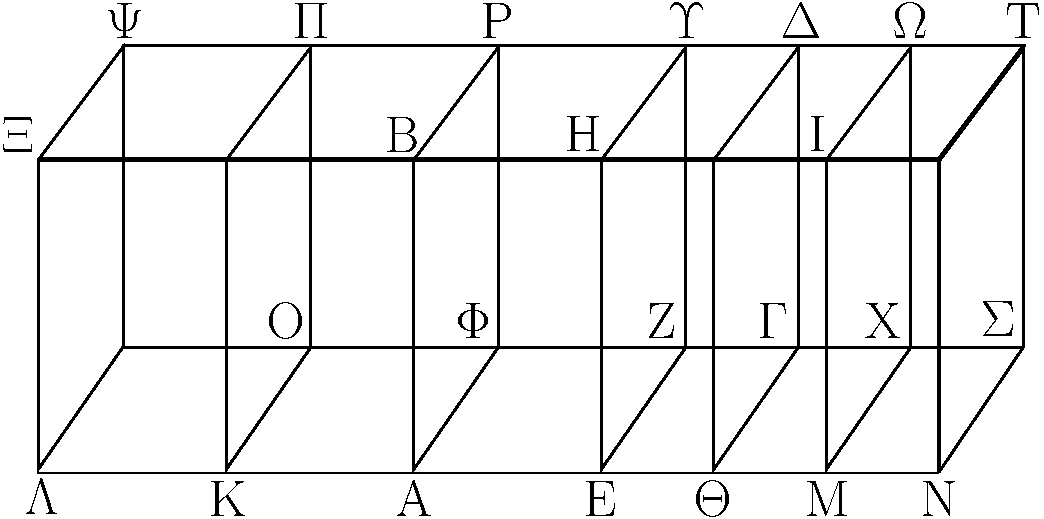
\includegraphics{Book11/fig25g.eps}}

\gr{Στερεὸν γὰρ παραλληλεπίπεδον τὸ ΑΒΓΔ ἐπιπέδῳ τῶ| ΖΗ τετμ\kern -.7pt  ήσθω
παραλλήλῳ >όντι τοῖξ ἀπεναντίον ἐπιπέδοιξ τοῖξ ΡΑ, ΔJ; λέγω,
<ότι ἐστὶν ὡξ ἡ ΑΕΖΦ βάσιξ πρὸξ τὴν ΕJΓΖ βάσιν, ο<ύτωξ
τὸ ΑΒΖΥ στερεὸν πρὸξ τὸ ΕΗΓΔ στερεόν.}

\gr{Ἐκβεβλήσθω γὰρ ἡ ΑJ ἐφ> ἑκάτερα τὰ μέρη, καὶ κείσθωσαν τῆ|
μὲν ΑΕ >ίσαι ὁσαιδηποτοῦν αἱ ΑΚ, ΚΛ, τῆ| δὲ ΕJ >ίσαι ὁσαιδηποτοῦν αἱ JΜ, ΜΝ, καὶ συμπεπληρώσθω τὰ ΛΟ, ΚΦ, JΘ, ΜΣ παραλληλόγραμμα καὶ τὰ ΛΠ, ΚΡ, ΔΜ, ΜΤ στερεά.}

\gr{Καὶ ἐπεὶ >ίσαι εἰσὶν αἱ ΛΚ, ΚΑ, ΑΕ εὐθεῖαι ἀλλήλαιξ,
 >ίσα  ἐστὶ
καὶ τὰ μὲν ΛΟ, ΚΦ, ΑΖ παραλληλόγραμμα ἀλλήλοιξ, τὰ δὲ ΚΧ, ΚΒ,
ΑΗ ἀλλήλοιξ καὶ >έτι τὰ ΛΨ, ΚΠ, ΑΡ ἀλλήλοιξ; ἀπεναντίον γάρ.
διὰ τὰ α\kern -.7pt  ὐτὰ δὴ καὶ τὰ μὲν ΕΓ, JΘ, ΜΣ παραλληλόγραμμα >ίσα
εἰσὶν ἀλλήλοιξ, τὰ δὲ JΗ, JΙ, ΙΝ >ίσα εἰσὶν ἀλλήλοιξ, καὶ >έτι
τὰ ΔJ, ΜΩ, ΝΤ; τρία >άρα ἐπίπεδα τῶν ΛΠ, ΚΡ, ΑΥ στερεῶν
τρισὶν ἐπιπέδοιξ ἐστὶν >ίσα. ἀλλὰ τὰ τρία τρισὶ τοῖξ ἀπεναντίον
ἐστὶν >ίσα; τὰ >άρα τρία στερεὰ τὰ ΛΠ, ΚΡ, ΑΥ >ίσα ἀλλήλοιξ
ἐστίν. διὰ τὰ α\kern -.7pt  ὐτὰ δὴ καὶ τὰ τρία στερεὰ τὰ ΕΔ, ΔΜ, ΜΤ >ίσα
ἀλλήλοιξ ἐστίν; ὁσαπλασίων >άρα ἐστὶν ἡ ΛΖ βάσιξ τῆξ ΑΖ βάσεωξ,
τοσαυταπλάσιόν ἐστι καὶ τὸ ΛΥ στερεὸν τοῦ ΑΥ στερεοῦ. διὰ τὰ
α\kern -.5pt  ὐτὰ δὴ ὁσαπλασίων ἐστὶν ἡ ΝΖ βάσιξ τῆξ ΖJ βάσεωξ,
τοσαυταπλάσιόν ἐστι καὶ τὸ ΝΥ στερεὸν τοῦ JΥ στερεοῦ. καὶ
εἰ >ίση ἐστὶν ἡ ΛΖ βάσιξ τῆ| ΝΖ βάσει, >ίσον ἐστὶ καὶ τὸ ΛΥ
στερεὸν τῶ| ΝΥ στερεῶ|, καὶ εἰ ὑπερέθει ἡ ΛΖ βάσιξ τῆξ ΝΖ
βάσεωξ, ὑπερέθει καὶ τὸ ΛΥ στερεὸν τοῦ ΝΥ στερεοῦ, καὶ εἰ
ἐλλείπει, ἐλλείπει. τεσσάρων δὴ >όντων μεγεθῶν, δύο μὲν βάσεων
τῶν ΑΖ, ΖJ, δύο δὲ στερεῶν τῶν ΑΥ, ΥJ,
ε>ίληπται ἰσάκιξ πολλαπλάσια τῆξ μὲν ΑΖ βάσεωξ καὶ τοῦ ΑΥ στερεοῦ
<ή τε ΛΖ βάσιξ καὶ τὸ ΛΥ στερεόν, τῆξ δὲ JΖ βάσεωξ καὶ τοῦ JΥ
στερεοῦ <ή τε ΝΖ βάσιξ καὶ τὸ ΝΥ
στερεόν, καὶ δέδεικται, <ότι εἱ ὑπερέθει ἡ ΛΖ βάσιξ τῆξ ΖΝ
βάσεωξ, ὑπερέθει καὶ τὸ ΛΥ στερεὸν τοῦ ΝΥ
 [στερεοῦ],  καὶ εἰ >ίση, >ίσον,
καὶ εἰ ἐλλείπει, ἐλλείπει. >έστιν >άρα ὡξ ἡ ΑΖ βάσιξ πρὸξ
τὴν ΖJ βάσιν, ο<ύτωξ τὸ ΑΥ στερεὸν πρὸξ τὸ ΥJ στερεόν; <όπερ
>έδει δεῖχαι.}}

\ParallelRText{
\begin{center}
{\large Proposition 25}
\end{center}

If a parallelipiped solid is cut by a plane which is 
parallel to the opposite planes (of the parallelipiped) then as the base (is) to
the base, so the solid will be to the solid.\\

\epsfysize=1.6in
\centerline{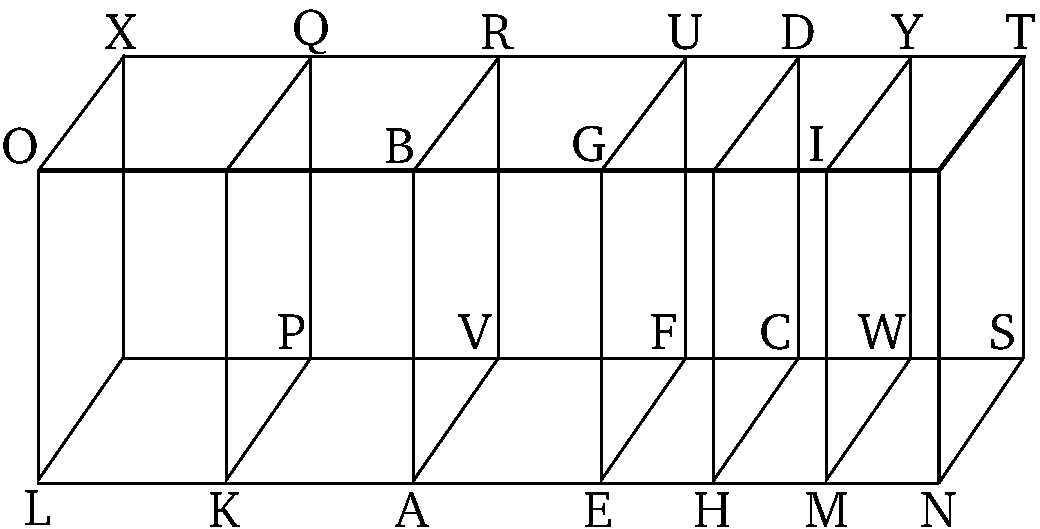
\includegraphics{Book11/fig25e.eps}}

For let the parallelipiped solid $ABCD$ be cut by the
plane $FG$ which is parallel to the opposite planes $RA$ and $DH$.
I say that as the base $AEFV$ (is) to the base $EHCF$, so the solid
$ABFU$ (is) to the solid $EGCD$.

For let $AH$ be produced in each direction. And let any number whatsoever (of lengths), $AK$ and $KL$, be made equal to $AE$,
and any number whatsoever (of lengths), $HM$ and $MN$, equal to $EH$.
And let the parallelograms $LP$, $KV$, $HW$, and $MS$ be completed, and the solids $LQ$, $KR$, $DM$, and $MT$.

And since the straight-lines $LK$, $KA$, and $AE$ are equal to one another,
the parallelograms $LP$, $KV$, and $AF$ are also equal to
one another, and $KO$, $KB$, and $AG$ (are equal) to one another, and,
further, $LX$, $KQ$, and $AR$ (are equal) to one another. For (they
are) opposite [Prop.~11.24]. So, for the
same (reasons), the parallelograms $EC$, $HW$, and $MS$
are also equal to one another, and $HG$, $HI$, and $IN$ are equal to
one another, and, further, $DH$, $MY$, and $NT$ (are equal to one another).
Thus, three planes of (one of) the solids $LQ$, $KR$, and $AU$ are equal to
the (corresponding) three planes (of the others). But, the three planes
(in one of the soilds) are equal to the three opposite planes [Prop.~11.24]. Thus, the three solids $LQ$,
$KR$, and $AU$ are equal to one another [Def.~11.10]. So, for the same (reasons), the
three solids $ED$, $DM$, and $MT$ are also equal to one another.
Thus, as many multiples as the base $LF$ is of the base $AF$, so many
multiples is the solid $LU$ also of the the solid $AU$. So, for the same (reasons), 
as many multiples as the base $NF$ is of the base $FH$, so many
multiples is the solid $NU$ also of the solid $HU$. And if the base
$LF$ is equal to the base $NF$ then the solid $LU$ is also
equal to the solid $NU$.$^\dag$ And if the base $LF$  exceeds the base $NF$
then the solid $LU$ also exceeds the solid $NU$. And if ($LF$) is less than ($NF$) then ($LU$) is (also) less than ($NU$). So, there are four magnitudes, the
two bases $AF$ and $FH$, and the two solids $AU$ and $UH$, and
equal multiples be taken of the base $AF$ and the solid $AU$--- (namely), the base $LF$ and the solid $LU$---and of the base
$HF$ and the solid $HU$---(namely), the base $NF$ and the solid $NU$.
And it has been shown that if the base $LF$ exceeds the base $FN$ then the
solid $LU$ also exceeds the [solid] $NU$, and if ($LF$ is) equal (to $FN$) then
($LU$ is) equal (to $NU$), and if ($LF$ is) less than ($FN$) then 
($LU$ is) less than ($NU$). Thus, as the base $AF$ is to the base
$FH$, so the solid $AU$ (is) to the solid $UH$ [Def.~5.5]. (Which is) the very thing it was required to show.}
\end{Parallel}
{\footnotesize\noindent$^\dag$ Here, Euclid assumes that $LF\gtreqqless NF$ implies $LU \gtreqqless NU$. This is easily demonstrated.}

%%%%
%11.26
%%%%
\pdfbookmark[1]{Proposition 11.26}{pdf11.26}
\begin{Parallel}{}{}
\ParallelLText{
\begin{center}
{\large \ggn{26}.}
\end{center}\vspace*{-7pt}

\gr{Πρὸξ τῆ| δοθείσῃ εὐθείᾳ καὶ τῶ| πρὸξ α\kern -.7pt  ὐτῆ| σημείῳ τῆ| δοθείσῃ
στερεᾶ| γωνίᾳ >ίσην στερεὰν γωνίαν συστήσασθαι.}

\gr{>'Εστω ἡ μὲν δοθεῖσα εὐθεῖα ἡ ΑΒ, τὸ δὲ πρὸξ α\kern -.7pt  ὐτῆ| δοθὲν
σημεῖον τὸ Α, ἡ δὲ δοθεῖσα στερεὰ γωνία ἡ πρὸξ τῶ| Δ περιεθομένη ὑπὸ τῶν ὑπὸ ΕΔΓ, ΕΔΖ, ΖΔΓ γωνιῶν ἐπιπέδων; δεῖ δὴ πρὸξ
τῆ| ΑΒ εὐθείᾳ καὶ τῶ| πρὸξ α\kern -.7pt  ὐτῆ| σημείῳ τῶ| Α τῆ| πρὸξ τῶ|
Δ στερεᾶ| γωνίᾳ >ίσην στερεὰν γωνίαν συστήσασθαι.}

\gr{Εἰλήφθω γὰρ ἐπὶ τῆξ ΔΖ τυθὸν σημεῖον τὸ Ζ, καὶ >ήθθω ἀπὸ
τοῦ Ζ ἐπὶ τὸ διὰ τῶν ΕΔ, ΔΓ ἐπίπεδον κάθετοξ ἡ ΖΗ, καὶ συμβαλλέτω τῶ| ἐπιπέδῳ κατὰ τὸ Η, καὶ ἐπεζεύθθω ἡ ΔΗ, καὶ
συνεστάτω πρὸξ τῆ| ΑΒ εὐθείᾳ καὶ τῶ| πρὸξ α\kern -.7pt  ὐτῆ| σημείῳ
τῶ| Α τῆ| μὲν ὑπὸ ΕΔΓ γωνίᾳ >ίση ἡ ὑπὸ ΒΑΛ, τῆ| δὲ
ὑπὸ ΕΔΗ >ίση ἡ ὑπὸ ΒΑΚ, καὶ κείσθω τῆ| ΔΗ >ίση  ἡ ΑΚ, καὶ
ἀνεστάτω ἀπὸ τοῦ Κ σημείου τῶ| διὰ τῶν ΒΑΛ ἐπιπέδῳ πρὸξ
ὀρθὰξ ἡ ΚJ, καὶ κείσθω >ίση τῆ| ΗΖ ἡ ΚJ, καὶ ἐπεζεύθθω ἡ JΑ;
λέγω, <ότι ἡ πρὸξ τῶ| Α στερεὰ γωνία περιεθομένη ὑπὸ τῶν
ΒΑΛ, ΒΑJ, JΑΛ γωνιῶν >ίση ἐστὶ τῆ| πρὸξ τῶ| Δ στερεᾶ|
γωνίᾳ τῆ| περιεθομένῃ ὑπὸ τῶν ΕΔΓ, ΕΔΖ, ΖΔΓ γωνιῶν.}

\epsfysize=1.8in
\centerline{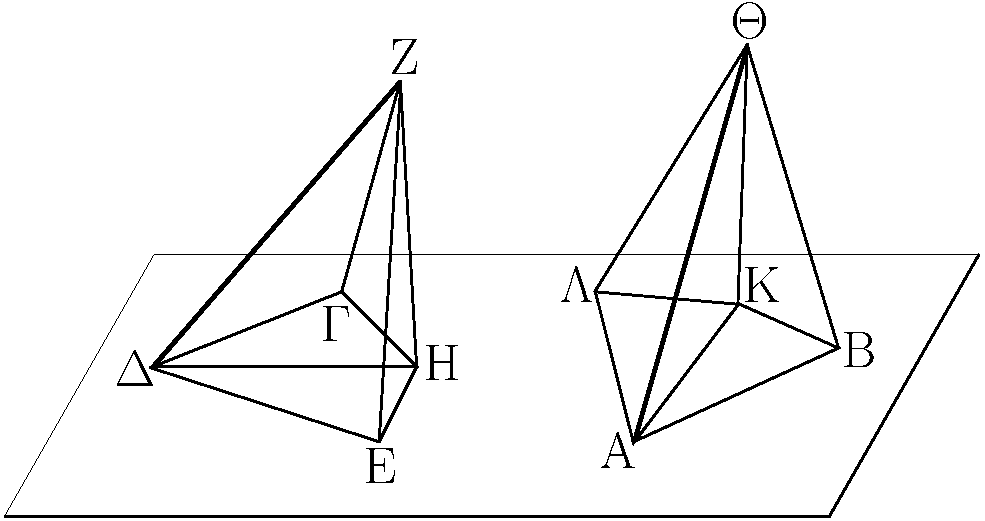
\includegraphics{Book11/fig26g.eps}}

\gr{Ἀπειλήφθωσαν γὰρ >ίσαι αἱ ΑΒ, ΔΕ, καὶ ἐπεζεύθj\-ωσαν αἱ JΒ, ΚΒ, ΖΕ, ΗΕ. καὶ ἐπεὶ ἡ ΖΗ ὀρθή ἐστι πρὸξ τὸ ὑποκείμενον ἐπίπεδον,
καὶ πρὸξ πάσαξ >άρα τὰξ ἁπτομέναξ α\kern -.7pt  ὐτῆξ εὐθείαξ καὶ ο>ύσαξ
ἐν τῶ| ὑποκειμένῳ ἐπιπέδῳ ὀρθὰξ ποιήσει γωνίαξ;
ὀρθὴ >άρα  ἐστὶν ἑκατέρα τῶν ὑπὸ ΖΗΔ, ΖΗΕ γωνιῶν. διὰ
τὰ α\kern -.7pt  ὐτὰ δὴ καὶ ἑκατέρα τῶν ὑπὸ JΚΑ, JΚΒ γωνιῶν ὀρθή ἐστιν.
καὶ ἐπεὶ δύο αἱ ΚΑ, ΑΒ δύο ταῖξ ΗΔ, ΔΕ >ίσαι εἰσὶν ἑκατέρα ἑκατέρᾳ, καὶ γωνίαξ >ίσαξ περιέθουσιν, βάσιξ >άρα ἡ ΚΒ βάσει τῆ|
ΗΕ >ίση ἐστίν. >έστι δὲ καὶ ἡ ΚJ τῆ| ΗΖ >ίση; καὶ γωνίαξ
ὀρθὰξ περιέθουσιν; >ίση >άρα καὶ ἡ JΒ τῆ| ΖΕ. πάλιν ἐπεὶ δύο
αἱ ΑΚ, ΚJ δυσὶ ταῖξ ΔΗ, ΗΖ >ίσαι εἰσίν, καὶ γωνίαξ ὀρθὰξ
περιέθουσιν, βάσιξ >άρα ἡ ΑJ βάσει τῆ| ΖΔ >ίση ἐστίν. >έστι δὲ
καὶ ἡ ΑΒ τῆ| ΔΕ >ίση; δύο δὴ αἱ JΑ, ΑΒ δύο ταῖξ ΔΖ, ΔΕ
>ίσαι εἰσίν. καὶ βάσιξ ἡ JΒ βάσει τῆ| ΖΕ >ίση; γωνία
>άρα ἡ ὑπὸ ΒΑJ γωνίᾳ τῆ| ὑπὸ ΕΔΖ ἐστιν >ίση. διὰ τὰ α\kern -.5pt  ὐτὰ
δὴ καὶ ἡ ὑπὸ JΑΛ τῆ| ὑπὸ ΖΔΓ ἐστιν >ίση. >έστι δὲ καὶ ἡ ὑπὸ
ΒΑΛ τῆ| ὑπὸ ΕΔΓ >ίση.}

\gr{Πρὸξ >άρα τῆ| δοθείσῃ εὐθείᾳ τῆ| ΑΒ καὶ τῶ| πρὸξ 	α\kern -.7pt  ὐτῆ|
σημείῳ τῶ| Α τῆ| δοθείσῃ στερεᾶ| γωνίᾳ τῆ| πρὸξ
τῶ| Δ >ίση συνέσταται; <όπερ >έδει ποιῆσαι.}}

\ParallelRText{
\begin{center}
{\large Proposition 26}
\end{center}

To construct a solid angle equal to a given solid
angle on a given straight-line, and at a given point on it.

Let $AB$ be the given straight-line, and $A$ the given point on it, and
$D$ the given solid angle, contained by the plane angles $EDC$, $EDF$, and
$FDC$. So, it is necessary to construct a solid angle equal to the solid angle $D$ on the straight-line $AB$, and at the point $A$ 
on it.

For let some random point $F$ be taken on $DF$, and let
$FG$ be drawn from $F$ perpendicular to the plane through $ED$ and
$DC$  [Prop.~11.11],  and let it meet the plane at $G$, and let $DG$ be joined.
And let $BAL$, equal to the angle $EDC$,  and $BAK$, equal to $EDG$, be constructed 
on the straight-line $AB$ at the point $A$ on it [Prop.~1.23]. And let $AK$ be made equal to $DG$.  And let $KH$
be set up at the point $K$ at right-angles to the plane through $BAL$
[Prop.~11.12]. And let $KH$ be made equal to
$GF$. And let $HA$ be joined. I say that the solid angle at $A$,
contained by the (plane) angles $BAL$, $BAH$, and $HAL$, is equal
to the solid angle at $D$, contained by the (plane) angles $EDC$,
$EDF$, and $FDC$.

\epsfysize=1.8in
\centerline{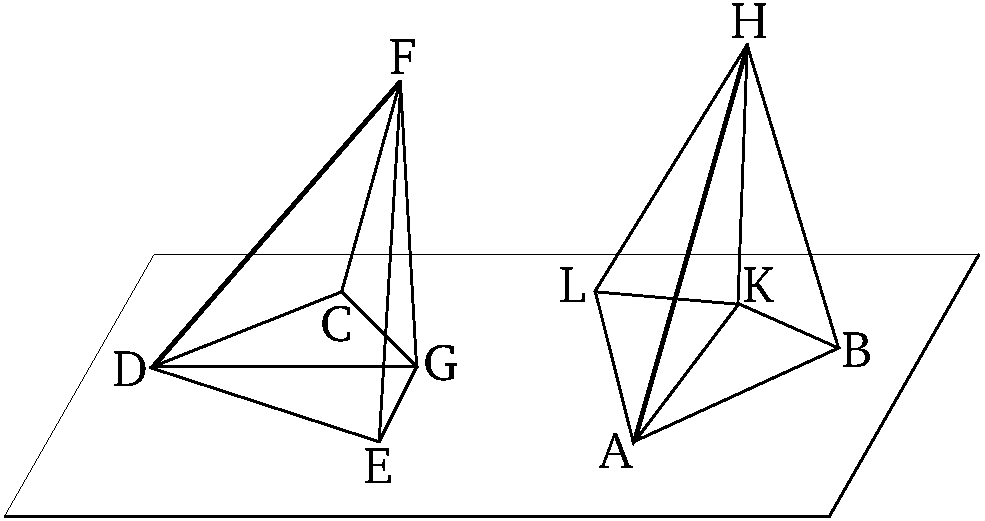
\includegraphics{Book11/fig26e.eps}}

For let $AB$ and $DE$ be cut off (so as to be) equal, and let
$HB$, $KB$, $FE$, and $GE$ be joined. And since $FG$
is at right-angles to the reference plane ($EDC$), it will also   make right-angles
with all of the straight-lines joined to it which are also in the reference
plane [Def.~11.3]. Thus, the angles $FGD$ and
$FGE$ are right-angles.  So, for the same (reasons), the angles $HKA$
and $HKB$ are also right-angles. And since the two (straight-lines)
$KA$ and $AB$ are equal to the two (straight-lines) $GD$ and $DE$,
respectively, and they contain equal angles, the base $KB$ is thus equal
to the base $GE$ [Prop.~1.4]. And $KH$ is also equal to $GF$. And they contain right-angles (with the respective bases). 
Thus, $HB$ (is) also equal to $FE$ [Prop.~1.4]. 
Again, since the two (straight-lines) $AK$ and $KH$ are equal to
the two (straight-lines) $DG$ and $GF$ (respectively), and they contain
right-angles, the base $AH$ is thus equal to the base $FD$ [Prop.~1.4].  And $AB$ (is) also equal to $DE$. So, the
two (straight-lines) $HA$ and $AB$ are equal to the two (straight-lines)
$DF$ and $DE$ (respectively).  And the base $HB$ (is) equal to the
base $FE$. Thus, the angle $BAH$ is equal to the angle $EDF$
[Prop.~1.8]. So, for the same (reasons),  $HAL$
is also equal to $FDC$. And $BAL$ is also equal to $EDC$.

Thus, (a solid angle) has been constructed, equal to the given solid angle at
$D$, on the given straight-line $AB$, at the given point $A$ on it.
(Which is) the very thing it was required to do.}
\end{Parallel}

%%%%
%11.27
%%%%
\pdfbookmark[1]{Proposition 11.27}{pdf11.27}
\begin{Parallel}{}{}
\ParallelLText{
\begin{center}
{\large \ggn{27}.}
\end{center}\vspace*{-7pt}

\gr{Ἀπὸ τῆξ δοθείσηξ εὐθείαξ τῶ| δοθέντι στερεῶ| παραλληλεπιπέδῳ
<όμοιόν τε καὶ ὁμοίωξ κείμενον στερεὸν παραλληλεπίπεδον
ἀναγράψαι.}

\gr{>'Εστω ἡ μὲν δοθεῖσα εὐθεῖα ἡ ΑΒ, τὸ δὲ δοθὲν στερεὸν
παραλληλεπίπεδον τὸ ΓΔ; δεῖ δὴ ἀπὸ τῆξ δοθείσηξ εὐθείαξ
τῆξ ΑΒ τῶ| δοθέντι στερεῶ| παραλληλεπιπέδῳ τῶ| ΓΔ
<όμοιόν τε καὶ ὁμοίωξ κείμενον στερεὸν παραλληλεπίπεδον
ἀναγράψαι.}

\gr{Συνεστάτω γὰρ πρὸξ τῆ|  ΑΒ εὐθείᾳ καὶ τῶ| πρὸξ α\kern -.7pt  ὐτῆ|
σημείῳ τῶ| Α τῆ| πρὸξ τῶ| Γ στερεᾶ| γωνίᾳ >ίση
ἡ περιεθομένη ὑπὸ τῶν ΒΑJ, JΑΚ, ΚΑΒ, <ώστε >ίσην ε>ῖναι τὴν
μὲν ὑπὸ ΒΑJ γωνίαν τῆ| ὑπὸ ΕΓΖ, τὴν δὲ ὑπὸ ΒΑΚ τῆ|
ὑπὸ ΕΓΗ, τὴν δὲ ὑπὸ ΚΑJ τῆ| ὑπὸ ΗΓΖ; καὶ γεγονέτω ὡξ μὲν
ἡ ΕΓ πρὸξ τὴν ΓΗ, ο<ύτωξ ἡ ΒΑ πρὸξ τὴν ΑΚ, ὡξ δὲ
ἡ ΗΓ πρὸξ τὴν ΓΖ,  ο<ύτωξ ἡ ΚΑ πρὸξ τὴν ΑJ. καὶ δι> >ίσου
>άρα ἐστὶν ὡξ ἡ ΕΓ πρὸξ τὴν ΓΖ, ο<ύτωξ ἡ ΒΑ πρὸξ
τὴν ΑJ. καὶ συμπεπληρώσθω τὸ JΒ παραλληλόγραμμον καὶ τὸ ΑΛ
στερεόν.}

\epsfysize=1.5in
\centerline{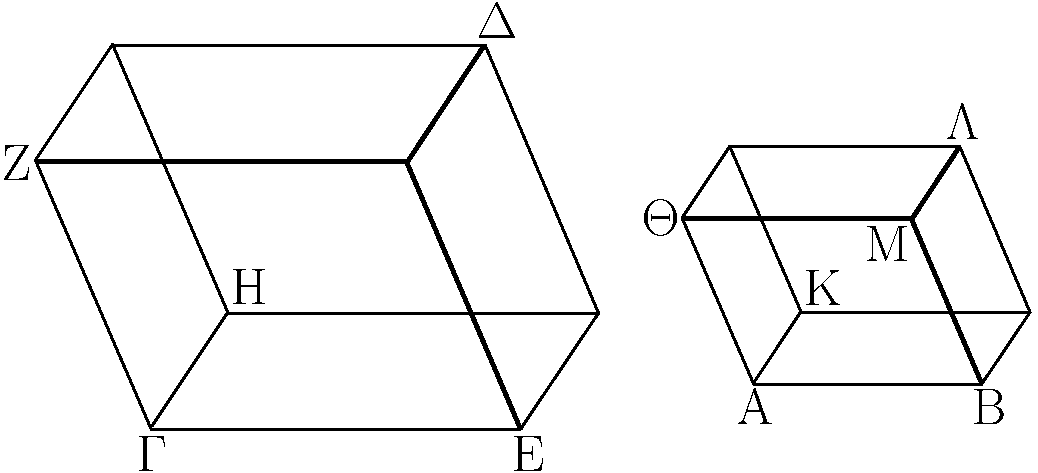
\includegraphics{Book11/fig27g.eps}}

\gr{Καὶ ἐπεί ἐστιν ὡξ ἡ ΕΓ πρὸξ τὴν ΓΗ, ο<ύτωξ ἡ ΒΑ
πρὸξ τὴν ΑΚ, καὶ περὶ >ίσαξ γωνίαξ τὰξ ὑπὸ ΕΓΗ, ΒΑΚ
αἱ πλευραὶ ἀνάλογόν εἰσιν, <όμοιον >άρα ἐστὶ τὸ ΗΕ
παραλληλόγραμμον τῶ| ΚΒ παραλληλογράμμῳ. διὰ τὰ α\kern -.7pt  ὐτὰ
δὴ καὶ τὸ μὲν ΚJ παραλληλόγραμμον τῶ| ΗΖ παραλληλογράμμῳ
<όμοιόν ἐστι καὶ >έτι τὸ ΖΕ τῶ| JΒ; τρία >άρα παραλληλόγραμμα τοῦ
ΓΔ στερεοῦ τρισὶ παραλληλογράμμοιξ τοῦ ΑΛ στερεοῦ <όμοιά ἐστιν.
ἀλλὰ τὰ μὲν τρία τρισὶ τοῖξ ἀπεναντίον >ίσα τέ ἐστι
καὶ <όμοια, τὰ δὲ τρία τρισὶ τοῖξ ἀπεναντίον
>ίσα τέ ἐστι καὶ <όμοια; <όλον >άρα τὸ ΓΔ στερεὸν <όλῳ τῶ|
ΑΛ στερεῶ| <όμοιόν ἐστιν.}

\gr{Ἀπὸ τῆξ δοθείσηξ >άρα εὐθείαξ τῆξ ΑΒ τῶ| δοθέντι
στερεῶ| παραλληλεπιπέδῳ τῶ| ΓΔ <όμοιόν τε καὶ ὁμοίωξ
κείμενον ἀναγέγραπται τὸ ΑΛ; <όπερ >έδει ποιῆσαι.}}

\ParallelRText{
\begin{center}
{\large Proposition 27}
\end{center}

To describe a parallelepiped solid similar,  and
similarly laid out, to a given parallelepiped solid on a given straight-line.

Let the given straight-line be $AB$, and the given parallelepiped solid
$CD$. So, it is necessary to describe a parallelepiped solid similar, and
similarly laid out, to the given parallelepiped solid $CD$ on the given straight-line $AB$.

For, let a (solid angle) contained by the (plane angles)
$BAH$, $HAK$, and $KAB$ be constructed, equal to solid angle at
$C$, on the straight-line $AB$ at the point $A$ on it [Prop.~11.26], such that angle $BAH$ is equal to $ECF$, and $BAK$ to $ECG$,
and $KAH$ to $GCF$. And let it be contrived that as $EC$
(is) to $CG$, so $BA$ (is) to $AK$, and as $GC$ (is) to $CF$, so
$KA$ (is) to $AH$ [Prop.~6.12]. And thus, via equality, as $EC$ is to $CF$, so
$BA$ (is) to $AH$ [Prop.~5.22]. And let the parallelogram $HB$ be completed, and the solid $AL$.

\epsfysize=1.5in
\centerline{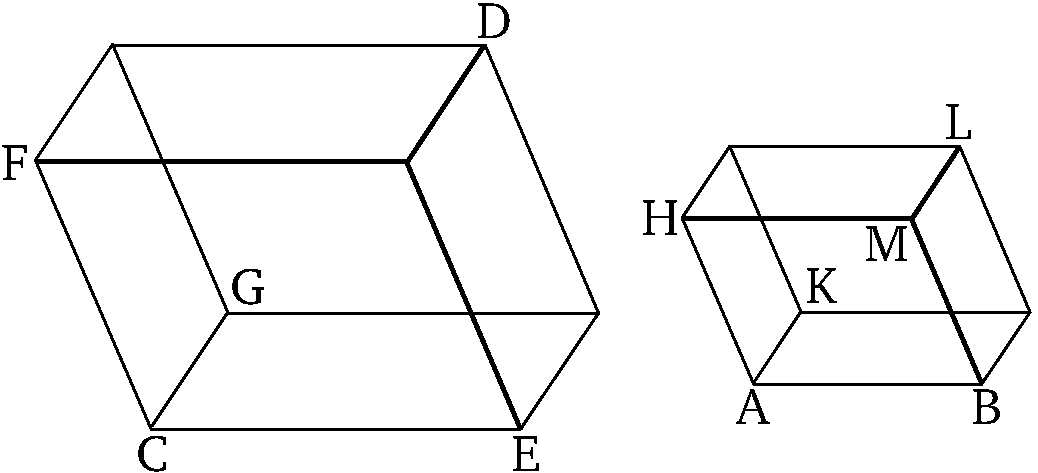
\includegraphics{Book11/fig27e.eps}}

And since as $EC$ is to $CG$, so $BA$ (is) to $AK$, and the sides about the equal angles $ECG$ and $BAK$ are (thus) proportional, the parallelogram
$GE$ is thus similar to the parallelogram $KB$. So, for the same (reasons),
the parallelogram $KH$ is also similar to the parallelogram $GF$, and,
further, $FE$ (is similar) to $HB$. Thus, three of the parallelograms
of solid $CD$ are similar to three of the parallelograms of solid $AL$.
But, the (former) three are equal and similar to the three opposite, and
the (latter) three are equal and similar to the three opposite. Thus, the
whole solid $CD$ is similar to the whole solid $AL$ [Def.~11.9].

Thus, $AL$, similar, and similarly laid out, to the given parallelepiped solid
$CD$, has been described on the given straight-lines $AB$. (Which is) the very thing it was required to do.}
\end{Parallel}

%%%%
%11.28
%%%%
\pdfbookmark[1]{Proposition 11.28}{pdf11.28}
\begin{Parallel}{}{}
\ParallelLText{
\begin{center}
{\large \ggn{28}.}
\end{center}\vspace*{-7pt}

\gr{Ἐὰν στερεὸν παραλληλεπίπεδον ἐπιπέδῳ τμ\kern -.7pt  ηθῆ| κατὰ τὰξ διαγωνίουξ
τῶν ἀπεναντίον ἐπιπέδων, δίθα τμ\kern -.7pt  ηθήσεται τὸ στερεὸν ὑπὸ τοῦ
ἐπιπέδου.}

\epsfysize=1.8in
\centerline{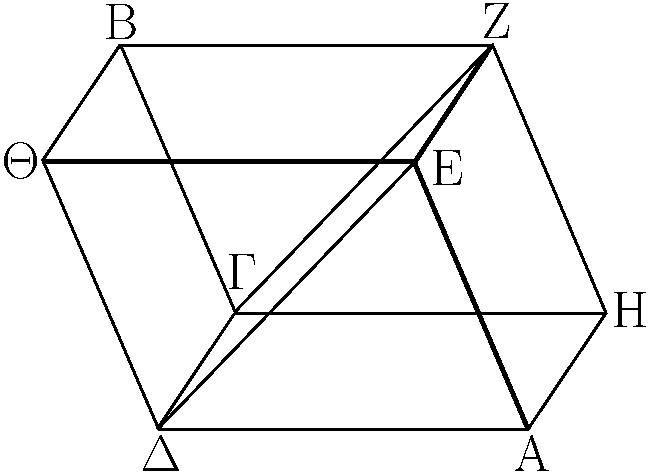
\includegraphics{Book11/fig28g.eps}}

\gr{Στερεὸν γὰρ παραλληλεπίπεδον τὸ ΑΒ ἐπιπέδῳ τῶ| ΓΔΕΖ τετμ\kern -.7pt  ήσθω
κατὰ τὰξ διαγωνίουξ τῶν ἀπεναντίον ἐπιπέδων τὰξ ΓΖ, ΔΕ;
λέγω, <ότι δίθα τμ\kern -.7pt  ηθήσεται τὸ ΑΒ στερεὸν ὑπὸ τοῦ ΓΔΕΖ
ἐπιπέδου.}

\gr{Ἐπεὶ γὰρ >ίσον ἐστὶ τὸ μὲν ΓΗΖ τρίγωνον τῶ| ΓΖΒ τριγώνῳ, τὸ δὲ ΑΔΕ τῶ| ΔΕJ, >έστι δὲ καὶ τὸ μὲν ΓΑ παραλληλόγραμμον τῶ| ΕΒ
>ίσον; ἀπεναντίον γάρ; τὸ δὲ ΗΕ τῶ| ΓJ, καὶ τὸ πρίσμα >άρα τὸ περιεχόμενον ὑπὸ δύο μὲν τριγώνων τῶν ΓΗΖ, ΑΔΕ, τριῶν δὲ παραλληλογράμμων τῶν ΗΕ, ΑΓ, ΓΕ >ίσον ἐστὶ τῶ| πρίσματι τῶ|
περιεθομένῳ ὑπὸ δύο μὲν τριγώνων τῶν ΓΖΒ, ΔΕJ, τριῶν
δὲ παραλληλογράμμων τῶν ΓJ, ΒΕ, ΓΕ; ὑπὸ γὰρ >ίσων ἐπιπέδων
περιέθονται τῶ| τε πλήθει καὶ τῶ| μεγέθει. <ώστε
<όλον τὸ ΑΒ στερεὸν δίθα τέτμ\kern -.7pt  ηται ὑπὸ τοῦ ΓΔΕΖ ἐπιπέδου;
<όπερ >έδει δεῖχαι.}}
 
\ParallelRText{
\begin{center}
{\large Proposition 28}
\end{center}

If a parallelepiped solid is cut by a plane (passing) through the diagonals of  (a pair of) opposite planes then the solid will be cut in half by the
plane.

\epsfysize=1.8in
\centerline{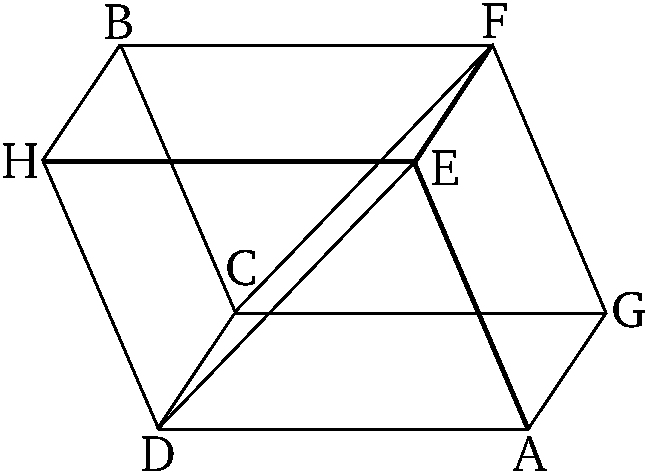
\includegraphics{Book11/fig28e.eps}}

For let the parallelepiped solid $AB$ be cut by the plane
$CDEF$ (passing) through the diagonals of the opposite planes $CF$ and $DE$.$^\dag$
I say that the solid $AB$ will be cut in half by the plane $CDEF$.

For since triangle $CGF$ is equal to triangle $CFB$, and $ADE$ (is equal)
to $DEH$ [Prop.~1.34], and parallelogram
$CA$ is also equal to $EB$---for (they are) opposite [Prop.~11.24]---and $GE$ (equal) to $CH$,  thus the prism contained
by the two triangles $CGF$ and $ADE$, and the three parallelograms $GE$, $AC$, and $CE$, is also equal to the prism contained by the two
triangles $CFB$ and $DEH$, and the three parallelograms $CH$, $BE$, and
$CE$. For they are contained by planes (which are) equal in number and in magnitude
[Def.~11.10].$^\ddag$ Thus, the whole of solid $AB$
is cut in half by the plane $CDEF$. (Which is) the very thing it was required to show.}
\end{Parallel}
{\footnotesize\noindent$^\dag$ Here, it is assumed that the two diagonals lie in the same plane. The proof is easily supplied.\\
\noindent$^\ddag$ However, strictly speaking, the prisms are not similarly arranged, being mirror images of one another.}

%%%%
%11.29
%%%%
\pdfbookmark[1]{Proposition 11.29}{pdf11.29}
\begin{Parallel}{}{}
\ParallelLText{
\begin{center}
{\large \ggn{29}.}
\end{center}\vspace*{-7pt}

\gr{Τὰ ἐπὶ τῆξ α\kern -.7pt  ὐτῆξ βάσεωξ >όντα στερεὰ παραλληλεπίπεδα καὶ ὑπὸ
τὸ α\kern -.7pt  ὐτὸ <ύψοξ, <ῶν αἱ ἐφεστῶσαι ἐπὶ τῶν α\kern -.5pt  ὐτῶν εἰσιν
εὐθειῶν, >ίσα ἀλλήλοιξ ἐστίν.}\\

\epsfysize=1.7in
\centerline{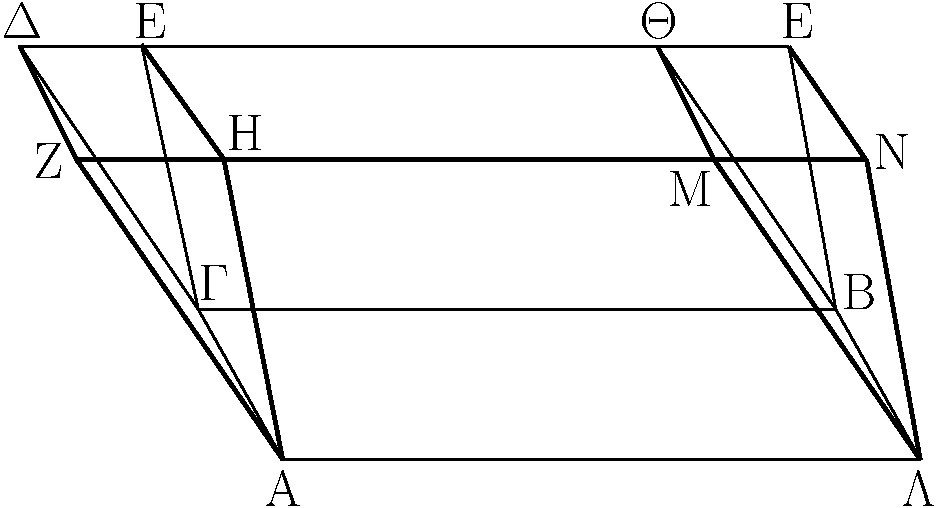
\includegraphics{Book11/fig29g.eps}}

\gr{>'Εστω ἐπὶ τῆξ α\kern -.7pt  ὐτῆξ βάσεωξ τῆξ ΑΒ στερεὰ παραλληλεπίπεδα τὰ ΓΜ,
ΓΝ ὑπὸ τὸ α\kern -.7pt  ὐτὸ <ύψοξ, <ῶν αἱ ἐφεστῶσαι αἱ ΑΗ, ΑΖ, ΛΜ,
ΛΝ, ΓΔ, ΓΕ, ΒJ, ΒΚ ἐπὶ τῶν α\kern -.5pt  ὐτῶν εὐθειῶν >έστωσαν
τῶν ΖΝ, ΔΚ; λέγω, <ότι >ίσον ἐστὶ τὸ ΓΜ στερεὸν τῶ| ΓΝ στερεῶ|.}

\gr{Ἐπεὶ γὰρ παραλληλόγραμμόν ἐστιν ἑκάτερον τῶν ΓJ, ΓΚ,
>ίση ἐστὶν ἡ ΓΒ ἑκατέρᾳ τῶν ΔJ, ΕΚ; <ώστε καὶ ἡ ΔJ
τῆ| ΕΚ ἐστιν >ίση. κοινὴ ἀφῃρήσθω ἡ ΕJ; λοιπὴ
>άρα ἡ ΔΕ λοιπῆ| τῆ| JΚ ἐστιν >ίση. <ώστε καὶ τὸ μὲν
ΔΓΕ τρίγωνον τῶ| JΒΚ τριγώνῳ >ίσον ἐστίν, τὸ δὲ ΔΗ
παραλληλόγραμμον τῶ| JΝ παραλληλογράμμῳ. διὰ τὰ α\kern -.7pt  ὐτὰ
δὴ καὶ τὸ ΑΖΗ τρίγωνον τῶ| ΜΛΝ τριγώνῳ >ίσον ἐστίν.
>έστι δὲ καὶ τὸ μὲν ΓΖ παραλληλόγραμμον τῶ| ΒΜ παραλληλογράμμῳ
>ίσον, τὸ δὲ ΓΗ τῶ| ΒΝ; ἀπεναντίον γάρ; καὶ τὸ πρίσμα
>άρα τὸ περιεχόμενον ὑπὸ δύο μὲν τριγώνων τῶν ΑΖΗ, ΔΓΕ,
τριῶν δὲ παραλληλογράμμων τῶν ΑΔ, ΔΗ, ΓΗ >ίσον ἐστὶ
τῶ| πρίσματι τῶ| περιεθομένῳ ὑπὸ δύο μὲν τριγώνων τῶν
ΜΛΝ, JΒΚ, τριῶν δὲ παραλληλογράμμων τῶν ΒΜ, JΝ,
ΒΝ. κοινὸν προσκείσθω τὸ στερεὸν, ο<ῦ βάσιξ μὲν τὸ ΑΒ
παραλληλόγραμμον, ἀπεναντίον δὲ τὸ ΗΕJΜ;
<όλον >άρα τὸ ΓΜ στερεὸν παραλληλεπίπεδον <όλῳ τῶ| ΓΝ
στερεῶ| παραλληλεπιπέδῳ >ίσον ἐστίν.}

\gr{Τὰ >άρα ἐπὶ τῆξ α\kern -.7pt  ὐτῆξ βάσεωξ >όντα στερεὰ παραλληλεπίπεδα
καὶ ὑπὸ τὸ α\kern -.7pt  ὐτὸ <ύψοξ, <ῶν αἱ ἐφεστῶσαι
ἐπὶ τῶν α\kern -.5pt  ὐτῶν εἰσιν εὐθειῶν, >ίσα ἀλλήλοιξ ἐστίν; <όπερ
>έδει δεῖχαι.}}

\ParallelRText{
\begin{center}
{\large Proposition 29}
\end{center}

Parallelepiped solids which are on the same base,
and (have) the same height, and in which the (ends of the straight-lines) standing up are on the same straight-lines, 
are equal to one another.

\epsfysize=1.7in
\centerline{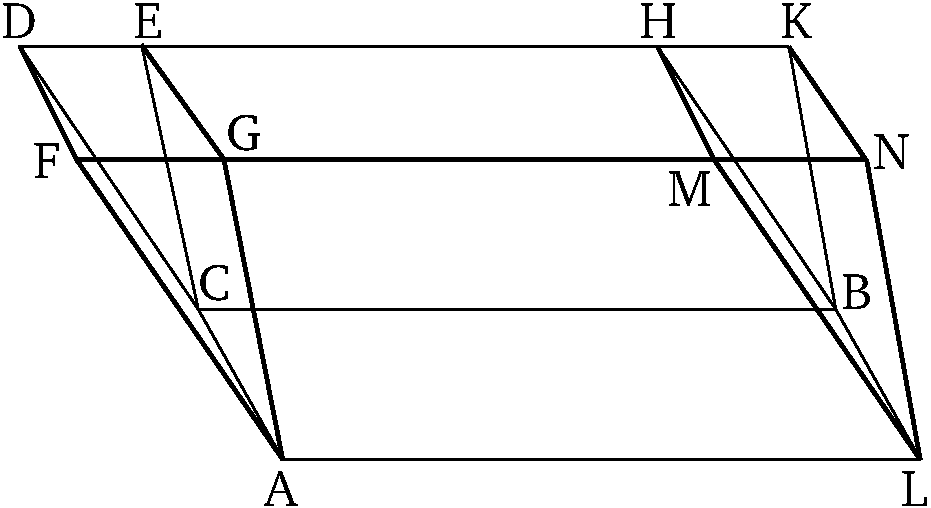
\includegraphics{Book11/fig29e.eps}}

For let the parallelepiped solids $CM$ and $CN$ be on the same base $AB$,
and (have) the same height, and let the (ends of the straight-lines)
standing up in them, $AG$, $AF$, $LM$, $LN$, $CD$, $CE$, $BH$, and $BK$,
be  on the same straight-lines, $FN$ and $DK$. I say that  solid $CM$
is equal to solid $CN$.

For since $CH$ and $CK$ are each parallelograms, $CB$ is equal to each 
of $DH$ and $EK$ [Prop.~1.34]. Hence,
$DH$ is also equal to $EK$. Let $EH$ be subtracted from both.
Thus, the remainder $DE$ is equal to the remainder $HK$.
Hence, triangle $DCE$ is also equal to triangle $HBK$ [Props.~1.4, 1.8], and parallelogram $DG$ to parallelogram $HN$
[Prop.~1.36]. So, for the same (reasons), traingle
$AFG$ is also equal to triangle $MLN$. And parallelogram $CF$ is
also equal to parallelogram $BM$, and $CG$ to $BN$ [Prop.~11.24]. For they are opposite. Thus, the prism contained by the
two triangles $AFG$ and $DCE$, and the three parallelograms $AD$,
$DG$, and $CG$, is equal to the prism contained by the two triangles
$MLN$ and $HBK$, and the three parallelograms $BM$, $HN$, and
$BN$. Let the solid whose base (is) parallelogram $AB$, and
(whose) opposite (face is) $GEHM$, be added to both (prisms).
Thus, the whole parallelepiped solid $CM$ is equal to the whole parallelepiped solid $CN$.

Thus, parallelepiped solids which are on the same base,
and (have) the same height, and in which the (ends of the straight-lines) standing up (are) on the same straight-lines, 
are equal to one another. (Which is) the very thing it was required to show.}
\end{Parallel}

%%%%
%11.30
%%%%
\pdfbookmark[1]{Proposition 11.30}{pdf11.30}
\begin{Parallel}{}{}
\ParallelLText{
\begin{center}
{\large \ggn{30}.}
\end{center}\vspace*{-7pt}

\gr{Τὰ ἐπὶ τῆξ α\kern -.7pt  ὐτῆξ βάσεωξ >όντα στερεὰ παραλληλεπίπεδα καὶ ὑπὸ
τὸ α\kern -.7pt  ὐτὸ <ύψοξ, <ῶν αἱ ἐφεστῶσαι οὐκ εἰσὶν ἐπὶ τῶν
α\kern -.5pt  ὐτῶν εὐθειῶν, >ίσα ἀλλήλοιξ ἐστίν.}\\

\epsfysize=2.2in
\centerline{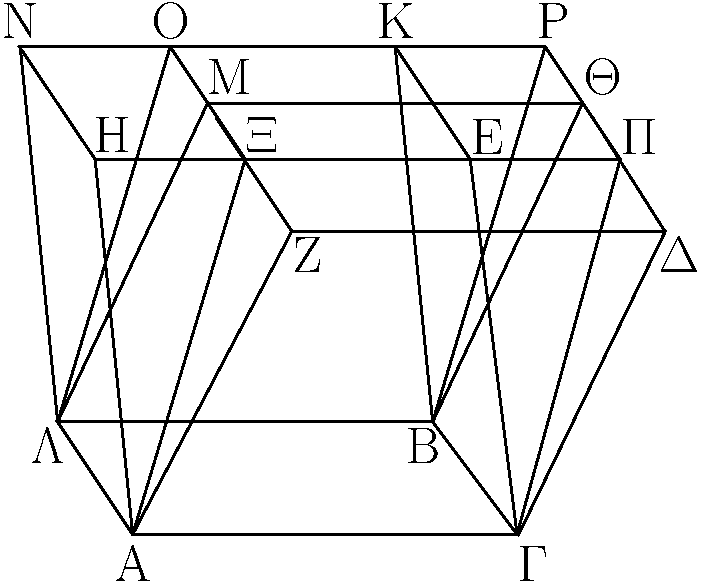
\includegraphics{Book11/fig30g.eps}}

\gr{>'Εστω ἐπὶ τῆξ α\kern -.7pt  ὐτῆξ βάσεωξ τῆξ ΑΒ στερεὰ παραλληλεπίπεδα
τὰ ΓΜ, ΓΝ ὑπὸ τὸ α\kern -.7pt  ὐτὸ <ύψοξ, <ῶν αἱ ἐφεστῶσαι αἱ ΑΖ,
ΑΗ, ΛΜ, ΛΝ, ΓΔ, ΓΕ, ΒJ, ΒΚ μ\kern -.5pt  ὴ >έστωσαν ἐπὶ τῶν α\kern -.3pt  ὐτῶν
εὐθειῶν; λέγω, <ότι >ίσον ἐστὶ τὸ ΓΜ στερεὸν τῶ| ΓΝ στερεῶ|.}

\gr{Ἐκβεβλήσθωσαν γὰρ αἱ ΝΚ, ΔJ καὶ συμπιπτέτωσαν ἀλλήλαιξ κατὰ
τὸ Ρ, καὶ >έτι ἐκβεβλήσθωσαν αἱ ΖΜ, ΗΕ ἐπὶ τὰ Ο, Π, καὶ
ἐπεζεύθθωσαν αἱ ΑΧ, ΛΟ, ΓΠ, ΒΡ. >ίσον δή ἐστι τὸ ΓΜ στερεόν,
ο<ῦ βάσιξ μὲν τὸ ΑΓΒΛ παραλληλόγραμμον, ἀπεναντίον δὲ τὸ
ΖΔJΜ, τῶ| ΓΟ στερεῶ|, ο<ῦ βάσιξ μὲν τὸ ΑΓΒΛ παραλληλόγραμμον,
ἀπεναντίον δὲ τὸ ΧΠΡΟ; ἐπί τε γὰρ τῆξ α\kern -.7pt  ὐτῆξ βάσεώξ εἰσι
τῆξ ΑΓΒΛ καὶ ὑπὸ τὸ α\kern -.7pt  ὐτὸ <ύψοξ, <ῶν αἱ ἐφεστῶσαι αἱ
ΑΖ, ΑΧ, ΛΜ, ΛΟ, ΓΔ, ΓΠ, ΒJ, ΒΡ ἐπὶ τῶν α\kern -.5pt  ὐτῶν εἰσιν
εὐθειῶν τῶν ΖΟ, ΔΡ. ἀλλὰ τὸ ΓΟ στερεόν, ο<ῦ βάσιξ
μέν ἐστι
τὸ ΑΓΒΛ παραλληλόγραμμον, ἀπεναντίον δὲ τὸ 
ΧΠΡΟ, >ίσον ἐστὶ τῶ| ΓΝ στερεῶ|, ο<ῦ βάσιξ μὲν τὸ
ΑΓΒΛ παραλληλόγραμμον, ἀπεναντίον δὲ τὸ
ΗΕΚΝ; ἐπί
τε γὰρ πάλιν τῆξ α\kern -.3pt  ὐτῆξ βάσεώξ εἰσι τῆξ ΑΓΒΛ καὶ
ὑπὸ τὸ α\kern -.7pt  ὐτὸ <ύψοξ, <ῶν αἱ ἐφεστῶσαι αἱ ΑΗ, ΑΧ, ΓΕ, ΓΠ,
ΛΝ, ΛΟ, ΒΚ, ΒΡ ἐπὶ τῶν α\kern -.7pt  ὐτῶν εἰσιν εὐθειῶν τῶν ΗΠ, ΝΡ. <ώστε
καὶ τὸ ΓΜ στερεὸν >ίσον ἐστὶ τῶ| ΓΝ στερεῶ|.}

\gr{Τὰ >άρα ἐπὶ τῆξ α\kern -.7pt  ὐτῆξ βάσεωξ  στερεὰ παραλληλεπίπεδα καὶ ὑπὸ
τὸ α\kern -.7pt  ὐτὸ <ύψοξ, <ῶν αἱ ἐφεστῶσαι οὐκ εἰσὶν ἐπὶ τῶν
α\kern -.5pt  ὐτῶν εὐθειῶν, >ίσα ἀλλήλοιξ ἐστίν; <όπερ >έδει δεῖχαι.}}

\ParallelRText{
\begin{center}
{\large Proposition 30}
\end{center}

Parallelepiped solids which are on the same base,
and (have) the same height, and in which the (ends of the straight-lines)
standing up are not on the same straight-lines, are equal to one another.

\epsfysize=2.2in
\centerline{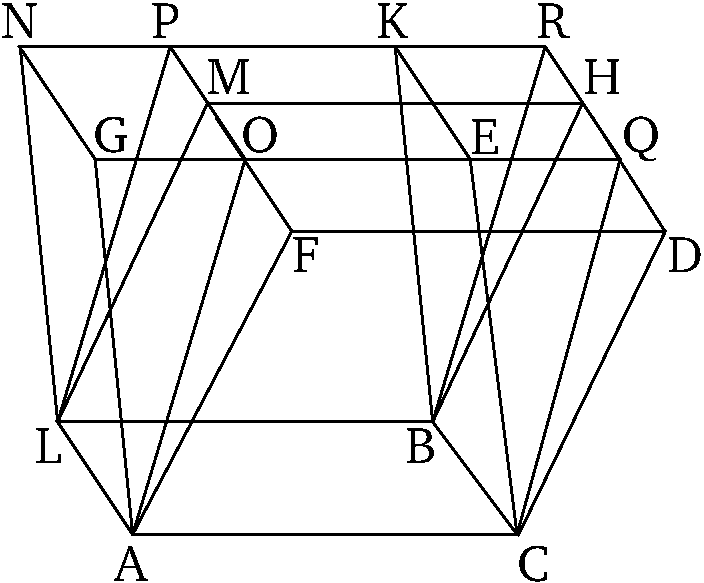
\includegraphics{Book11/fig30e.eps}}

Let the parallelepiped solids $CM$ and $CN$ be on the same base, $AB$,
and (have) the same height, and let the (ends of the straight-lines)
standing up in them, $AF$, $AG$, $LM$, $LN$, $CD$, $CE$, $BH$,
and $BK$, not be on the same straight-lines. I say that the solid $CM$
is equal to the solid $CN$.

For let $NK$ and $DH$ be produced, and let them have joined
one another at $R$. And, further, let $FM$ and $GE$ be produced
to $P$ and $Q$ (respectively). And let $AO$, $LP$, $CQ$, and
$BR$ be joined. So, solid $CM$, whose base (is)
parallelogram $ACBL$, and opposite (face) $FDHM$, is equal to solid
$CP$, whose base (is) parallelogram $ACBL$, and opposite
(face) $OQRP$. For they are on the same base, $ACBL$, and (have) the
same height, and the (ends of the straight-lines) standing up in them,
$AF$, $AO$, $LM$, $LP$, $CD$, $CQ$, $BH$, and $BR$, are on the
same straight-lines, $FP$ and $DR$ [Prop.~11.29]. 
But,  solid $CP$, whose base is parallelogram
$ACBL$, and opposite (face) $OQRP$, is equal to solid
$CN$, whose base (is) parallelogram $ACBL$, and opposite (face)
$GEKN$. For, again, they are on the same base, $ACBL$,
and (have) the same height, and the (ends of the straight-lines) standing up
in them, $AG$, $AO$, $CE$, $CQ$, $LN$, $LP$, $BK$, and $BR$,
are on the same straight-lines, $GQ$ and $NR$ [Prop.~11.29]. Hence, solid $CM$ is also equal to solid $CN$.

Thus, parallelepiped solids (which are) on the same base,
and (have) the same height, and in which the (ends of the straight-lines)
standing up are not on the same straight-lines, are equal to one another.
(Which is) the very thing it was required to show.}
\end{Parallel}

%%%%
%11.31
%%%%
\pdfbookmark[1]{Proposition 11.31}{pdf11.31}
\begin{Parallel}{}{}
\ParallelLText{
\begin{center}
{\large \ggn{31}.}
\end{center}\vspace*{-7pt}

\gr{Τὰ ἐπὶ >ίσων βάσεων >όντα στερεὰ παραλληλεπίπεδα καὶ ὑπὸ
τὸ α\kern -.7pt  ὐτὸ <ύψοξ >ίσα ἀλλήλοιξ ἐστίν.}

\gr{>'Εστω ἐπὶ >ίσων βάσεων τῶν ΑΒ, ΓΔ στερεὰ παραλληλεπίπεδα
τὰ ΑΕ, ΓΖ ὑπὸ τὸ α\kern -.7pt  ὐτὸ <ύψοξ. λέγω, <ότι >ίσον ἐστὶ τὸ ΑΕ
στερεὸν τῶ| ΓΖ στερεῶ|.}

\gr{>'Εστωσαν δὴ πρότερον αἱ ἐφεστηκυῖαι αἱ JΚ, ΒΕ, ΑΗ, ΛΜ, ΟΠ,
ΔΖ, ΓΧ, ΡΣ πρὸξ ὀρθὰξ ταῖξ ΑΒ, ΓΔ βάσεσιν, καὶ ἐκβεβλήσθω
ἐπ> εὐθείαξ τῆ| ΓΡ εὐθεῖα ἡ ΡΤ, καὶ συνεστάτω πρὸξ τῆ|
ΡΤ εὐθείᾳ καὶ τῶ| πρὸξ α\kern -.7pt  ὐτῆ| σημείῳ τῶ| Ρ τῆ| ὑπὸ ΑΛΒ
γωνίᾳ >ίση ἡ ὑπὸ ΤΡΥ, καὶ κείσθω τῆ| μὲν ΑΛ >ίση ἡ ΡΤ,
τῆ| δὲ ΛΒ >ίση ἡ ΡΥ, καὶ συμπεπληρώσθω <ή τε ΡΘ βάσιξ
καὶ τὸ ΨΥ στερεόν.}

\epsfysize=4in
\centerline{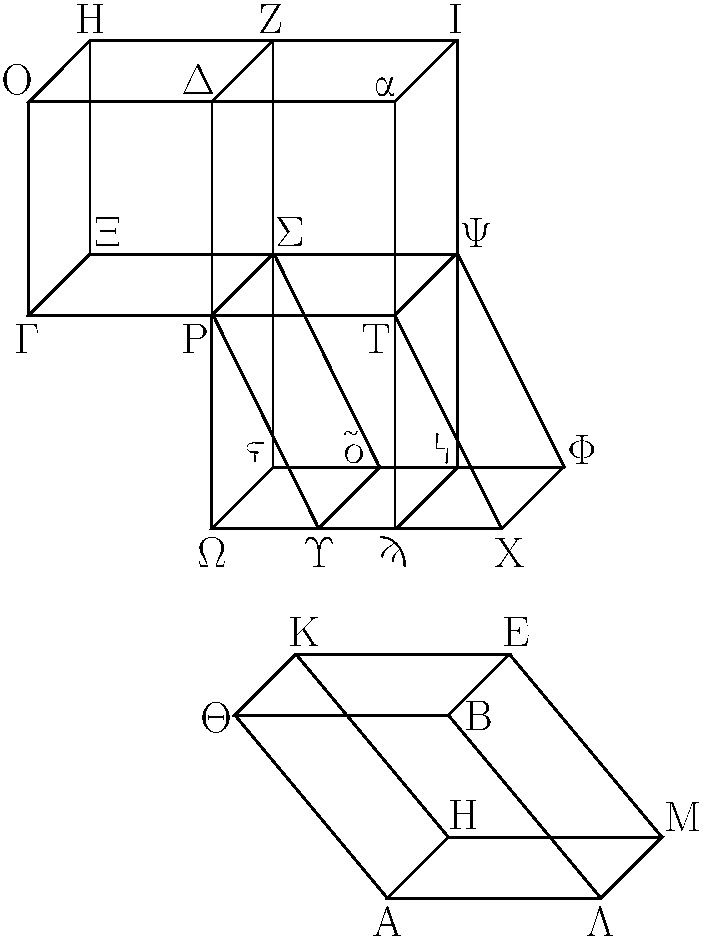
\includegraphics{Book11/fig31g.eps}}

\gr{Καὶ ἐπεὶ δύο αἱ ΤΡ, ΡΥ δυσὶ ταῖξ ΑΛ,
ΛΒ >ίσαι εἰσίν, καὶ γωνίαξ >ίσαξ περιέθουσιν, >ίσον >άρα
καὶ <όμοιον τὸ ΡΘ παραλληλόγραμμον τῶ| JΛ παραλληλογράμμῳ.
καὶ ἐπεὶ πάλιν >ίση μὲν ἡ ΑΛ τῆ| ΡΤ, ἡ δὲ ΛΜ τῆ| ΡΣ, καὶ
γωνίαξ ὀρθὰξ περιέθουσιν, >ίσον >άρα καὶ <όμοιόν ἐστι
τὸ ΡΨ παραλληλόγραμμον τῶ| ΑΜ παραλληλογράμμῳ. διὰ τὰ
α\kern -.7pt  ὐτὰ δὴ καὶ τὸ ΛΕ τῶ| ΣΥ >ίσον τέ ἐστι καὶ <όμοιον;
τρία >άρα παραλληλόγραμμα τοῦ ΑΕ στερεοῦ τρισὶ παραλληλογράμμοιξ
τοῦ ΨΥ στερεοῦ >ίσα τέ ἐστι καὶ <όμοια. ἀλλὰ τὰ μὲν τρία
τρισὶ τοῖξ ἀπεναντίον >ίσα τέ ἐστι καὶ <όμοια, τὰ δὲ τρία τρισὶ
τοῖξ ἀπεναντίον; <όλον >άρα τὸ ΑΕ στερεὸν παραλληλεπίπεδον
<όλῳ τῶ| ΨΥ στερεῶ| παραλληλεπιπέδῳ >ίσον ἐστίν. διήθθωσαν
αἱ ΔΡ, ΘΥ καὶ συμπιπτέτωσαν ἀλλήλαιξ κατὰ τὸ Ω,
καὶ διὰ τοῦ Τ τῆ| ΔΩ παράλληλοξ >ήθθω ἡ αΤ\kern -.7pt ,
καὶ ἐκβεβλήσθω ἡ ΟΔ κατὰ τὸ α, καὶ συμπεπληρώσθω τὰ ΩΨ, ΡΙ στερεά. >ίσον δή ἐστι τὸ ΨΩ στερεόν, ο<ῦ βάσιξ μέν ἐστι τὸ
ΡΨ παραλληλόγραμμον, ἀπεναντίον
δὲ τὸ Ω\kern -.5pt , τῶ| ΨΥ στερεῶ|, ο<ῦ βάσιξ μὲν τὸ ΡΨ παραλληλόγραμμον, ἀπεναντίον δὲ τὸ ΥΦ; ἐπί τε γὰρ τῆξ α\kern -.3pt  ὐτῆξ
βάσεώξ εἰσι τῆξ ΡΨ καὶ ὑπὸ τὸ α\kern -.7pt  ὐτὸ <ύψοξ, <ῶν αἱ
ἐφεστῶσαι αἱ ΡΩ, ΡΥ, Τ\kern -.7pt , ΤΘ, Σ\kern -.7pt , Σ$\kern -.7pt {\kern -.7pt {ο}}$, Y\qoppa,
YF >ep`i t~wn a\kern -.7pt >ut~wn e>isin e>ujei~wn t~wn WQ, \stigma F. >all`a
t`o YU stere`on t~w| AE >estin >'ison; ka`i t`o YW >'ara stere`on t~w|
AE stere~w| >estin >'ison. ka`i >epe`i >'ison >est`i t`o RUQT
parallhl'ogrammon t~w| WT parallhlogr'ammw|; >ep'i te g`ar t~hc
a\kern -.7pt >ut~hc b'ase'wc e>isi t~hc RT ka`i >en ta~ic a\kern -.7pt >uta~ic
parall'hloic ta~ic RT, WQ; >all`a t`o RUQT t~w| GD >estin >'ison,
>epe`i ka`i t~w| AB, ka`i t`o WT >'ara parallhl'ogrammon t~w| GD
>estin >'ison. >'allo d`e t`o DT; >'estin >'ara <wc <h GD b'asic
pr`oc t`hn DT, o<'utwc <h WT pr`oc t`hn DT. ka`i >epe`i
stere`on parallhlep'ipedon t`o GI >epip'edw| t~w| RZ  t'etm\kern -.7pt htai parall'hlw|
>'onti to~ic >apenant'ion >epip'edoic, >'estin <wc <h GD b'asic
pr`oc t`hn DT b'asin, o<'utwc t`o GZ stere`on pr`oc t`o RI
stere'on. di`a t`a a\kern -.7pt >ut`a d'h, >epe`i stere`on parallhlep'ipedon t`o WI
>epip'edw| t~w| RY t'etm\kern -.7pt htai parall'hlw| >'onti to~ic >apenant'ion
>epip'edoic, >'estin <wc <h WT b'asic pr`oc t`hn TL b'asin, o<'utwc
t`o WY
stere`on pr`oc t`o RI. >all> <wc <h GD
b'asic pr`oc t`hn DT, o<'utwc <h WT pr`oc t`hn DT; ka`i
<wc >'ara t`o GZ stere`on pr`oc t`o RI stere'on, o<'utwc t`o WY
stere`on pr`oc t`o RI. <ek'ateron >'ara t~wn GZ, WY stere~wn pr`oc t`o RI
t`on a\kern -.7pt >ut`on >'eqei l'ogon; >'ison >'ara >est`i t`o GZ stere`on
t~w| WY stere~w|. >all`a t`o WY t~w| AE >ede'iqjh >'ison; ka`i t`o AE
>'ara t~w| GZ >estin >'ison.}\\

\epsfysize=1.8in
\centerline{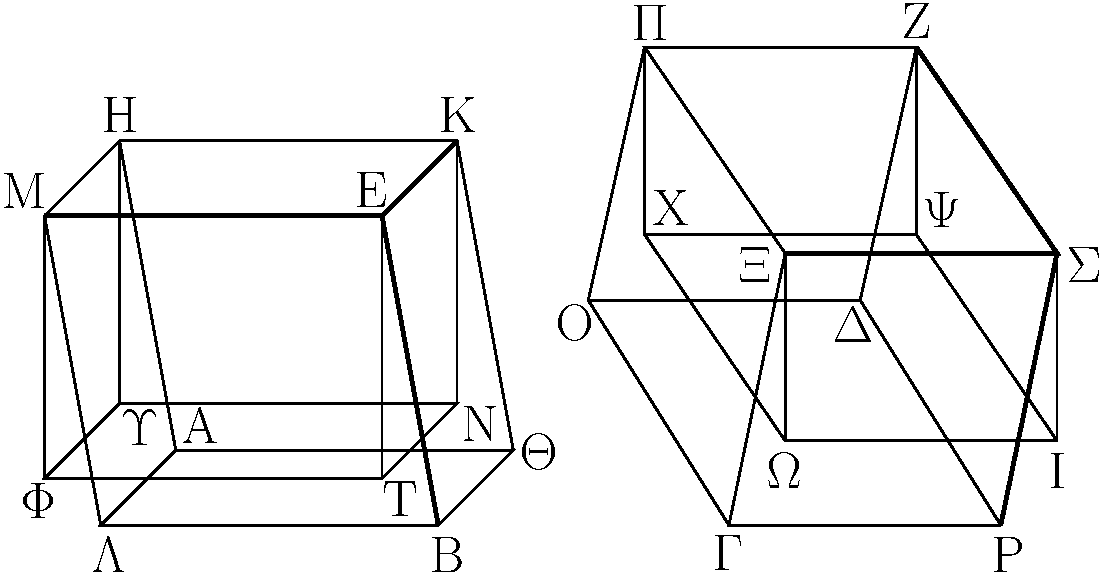
\includegraphics{Book11/fig31ag.eps}}

\gr{μ\kern -.7pt  ὴ >έστωσαν δὴ αἱ ἐφεστηκυῖαι αἱ ΑΗ, JΚ, ΒΕ, ΛΜ, ΓΧ, ΟΠ,
ΔΖ, ΡΣ πρὸξ ὀρθὰξ ταῖξ ΑΒ, ΓΔ βάσεσιν; λέγω πάλιν, <ότι
<ίσον τὸ ΑΕ στερεὸν τῶ| ΓΖ στερεῶ|. >ήθθωσαν γὰρ ἀπὸ τῶν Κ,
Ε, Η, Μ, Π, Ζ, Χ, Σ σημείων ἐπὶ τὸ ὑποκείμενον ἐπίπεδον κάθετοι
αἱ ΚΝ, ΕΤ, ΗΥ, ΜΦ, ΠΘ, ΖΨ, ΧΩ, ΣΙ, καὶ συμβαλλέτωσαν τῶ| ἐπιπέδῳ
κατὰ τὰ Ν, Τ, Υ, Φ, Θ, Ψ, Ω, Ι σημεῖα, καὶ ἐπεζεύθθωσαν αἱ ΝΤ, ΝΥ,
ΥΦ, ΤΦ, ΘΨ, ΘΩ, ΩΙ, ΙΨ. >ίσον δή ἐστι τὸ ΚΦ στερεὸν τῶ| ΠΙ
στερεῶ|; ἐπί τε γὰρ >ίσων βάσεών εἰσι τῶν ΚΜ, ΠΣ καὶ
ὑπὸ τὸ α\kern -.7pt  ὐτὸ <ύψοξ, <ῶν αἱ ἐφεστῶσαι πρὸξ ὀρθάξ
εἰσι ταῖξ βάσεσιν. ἀλλὰ τὸ μὲν ΚΦ στερεὸν τῶ| ΑΕ στερεῶ|
ἐστιν >ίσον, τὸ δὲ ΠΙ τῶ| ΓΖ; ἐπί τε γὰρ τῆξ α\kern -.5pt  ὐτῆξ βάσεώξ
εἰσι καὶ ὑπὸ τὸ α\kern -.3pt  ὐτὸ <ύψοξ, <ῶν αἱ ἐφεστῶσαι ο>ύκ εἰσιν
ἐπὶ τῶν α\kern -.7pt  ὐτῶν εὐθειῶν. καὶ τὸ ΑΕ >άρα στερεὸν τῶ|
ΓΖ στερεῶ| ἐστιν >ίσον.}

\gr{Τὰ >άρα ἐπὶ >ίσων βάσεων >όντα στερεὰ παραλληλεπίπεδα καὶ
ὑπὸ τὸ α\kern -.7pt  ὐτὸ <ύψοξ >ίσα ἀλλήλοιξ
ἐστίν; <όπερ >έδει δεῖχαι.}}

\ParallelRText{
\begin{center}
{\large Proposition 31}
\end{center}

Parallelepiped solids which are on equal bases,
and (have) the same height, are equal to one another.

Let the parallelepiped solids $AE$ and $CF$ be on the equal bases $AB$
and $CD$ (respectively), and (have) the same height. I say that solid
$AE$ is equal to solid $CF$.

 So, let the
(straight-lines) standing up, $HK$, $BE$, $AG$, $LM$, $PQ$, $DF$,
$CO$, and $RS$, first of all, be at right-angles to the bases $AB$
and $CD$. And let $RT$ be produced in a straight-line with
$CR$. And let  (angle) $TRU$, equal to angle $ALB$, be
constructed on the straight-line $RT$, at the point $R$ on it [Prop.~1.23]. And let
$RT$ be made equal to $AL$, and $RU$ to $LB$. And let the base
$RW$, and the solid $XU$,  be completed.

\epsfysize=4in
\centerline{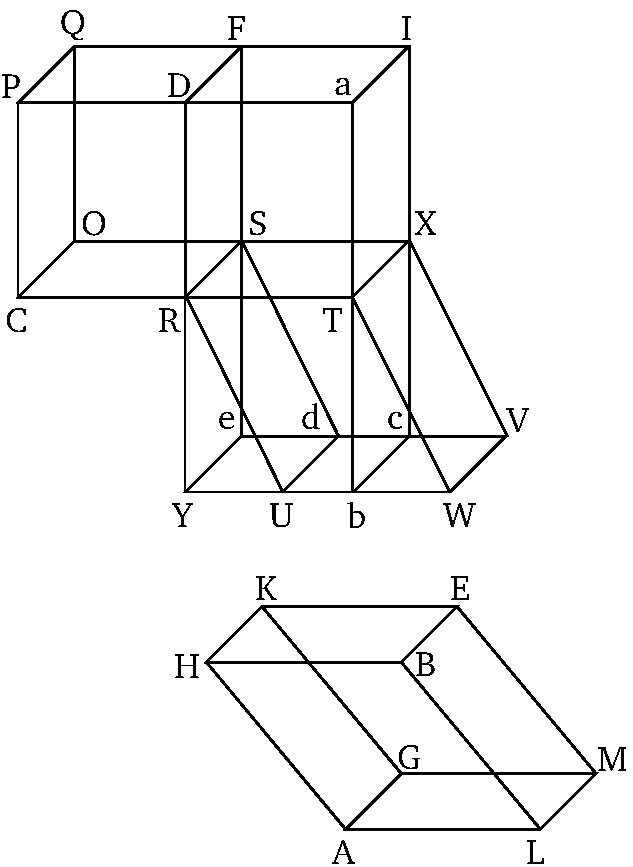
\includegraphics{Book11/fig31e.eps}}

And since the two (straight-lines) $TR$ and $RU$ are
equal to the two (straight-lines) $AL$ and $LB$ (respectively), and
they contain equal angles, parallelogram $RW$ is thus  equal
and similar to parallelogram $HL$ [Prop.~6.14]. 
And, again, since $AL$ is equal to $RT$, and $LM$ to $RS$, and they contain right-angles, parallelogram $RX$ is thus equal and similar to
parallelogram $AM$ [Prop.~6.14].  So, for the
same (reasons), $LE$ is also equal and similar to $SU$. Thus, three
parallelograms of solid $AE$ are equal and similar to three parallelograms of
 solid $XU$. But, the three (faces of the former solid)
are equal and similar to the three opposite (faces), and the three (faces
of the
latter solid) to the three opposite (faces) [Prop.~11.24]. Thus, the whole
parallelepiped solid $AE$ is equal to the whole parallelepiped solid
$XU$ [Def.~11.10]. Let $DR$ and
$WU$ be drawn across, and let them have met one another at $Y$.
And let $aTb$ be drawn through $T$ parallel to $DY$. And let
$PD$ be produced to $a$. And let the solids $YX$ and $RI$ be 
completed. So,  solid $XY$, whose base is parallelogram $RX$,
and opposite (face) $Yc$,  is equal to  solid $XU$, whose base
(is) parallelogram $RX$, and opposite (face) $UV$. For they are
on the same base $RX$, and (have) the same height,  and the (ends of the straight-lines) standing up in them, $RY$, $RU$, $Tb$, $TW$, $Se$, $Sd$, $Xc$ and $XV$, are on the same straight-lines, $YW$ and $eV$ 
[Prop.~11.29].  But, solid $XU$ is equal to
$AE$. Thus, solid $XY$ is also equal to solid $AE$. And since
parallelogram $RUWT$ is equal to parallelogram $YT$. For they are
on the same base $RT$, and between the same parallels $RT$ and $YW$
[Prop.~1.35]. But, $RUWT$ is equal to
$CD$, since (it is) also (equal) to $AB$. Parallelogram $YT$ is thus also
equal to $CD$. And $DT$ is another (parallelogram). Thus, as base $CD$
is to $DT$, so $YT$ (is) to $DT$ [Prop.~5.7]. 
And since the parallelepiped solid $CI$ has been cut by the plane
$RF$, which is parallel to the opposite planes (of $CI$), as  base $CD$
is to base $DT$, so solid $CF$ (is) to solid $RI$ [Prop.~11.25]. So, for the same (reasons), since the parallelepiped solid
$YI$ has been cut by the plane $RX$, which is parallel to the opposite
planes (of $YI$), as base $YT$ is to base $TD$, so solid $YX$ (is)
 to solid $RI$ [Prop.~11.25]. But, as base $CD$ (is) to $DT$, so $YT$ (is) to $DT$. And, thus, as solid $CF$ (is) to solid $RI$,
so solid $YX$ (is) to solid $RI$. Thus,  solids $CF$ and
$YX$ each have the same ratio to $RI$ [Prop.~5.11]. Thus, solid $CF$
is equal to solid $YX$ [Prop.~5.9]. But,
$YX$ was show (to be) equal to $AE$. Thus, $AE$ is also equal to
$CF$.

\epsfysize=1.8in
\centerline{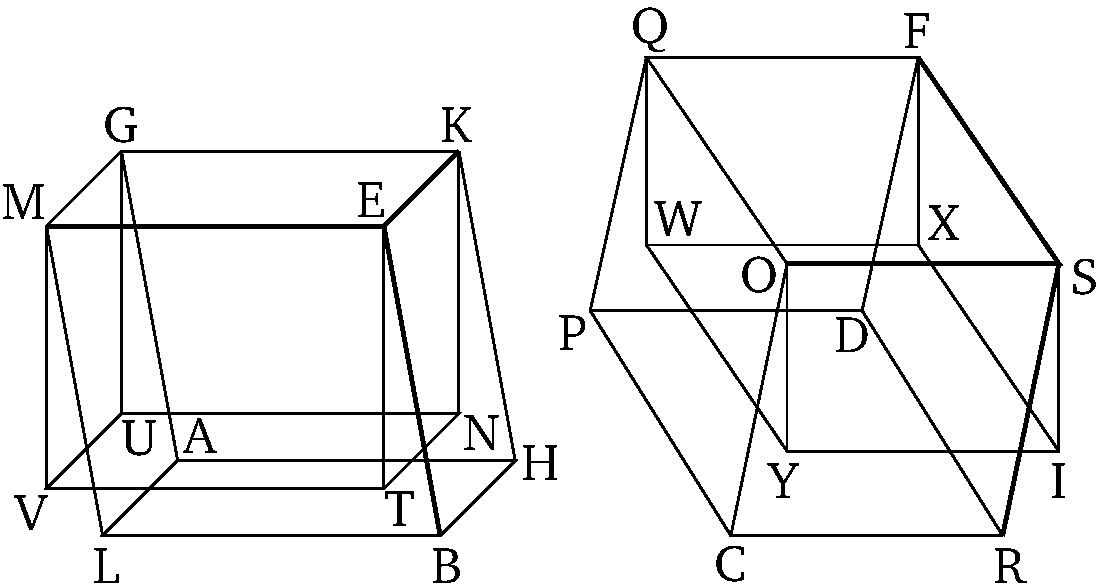
\includegraphics{Book11/fig31ae.eps}}

And so let the (straight-lines) standing up, $AG$, $HK$, $BE$,
$LM$, $CO$, $PQ$, $DF$, and $RS$, not be at right-angles to
the bases $AB$ and $CD$. Again, I say that solid $AE$ (is) equal to
solid  $CF$. For let $KN$, $ET$, $GU$, $MV$, $QW$, $FX$, $OY$, and
$SI$ be drawn from points $K$, $E$, $G$, $M$, $Q$, $F$, $O$, and
$S$ (respectively) perpendicular to the reference plane ({\rm  i.e.}, the plane of the bases $AB$ and $CD$), and let them have met
the plane at points $N$, $T$, $U$, $V$, $W$, $X$, $Y$, and $I$ (respectively). And let $NT$, $NU$, $UV$, $TV$, $WX$, $WY$, $YI$, and
$IX$ be joined. So solid $KV$ is equal to solid $QI$. For they are on
the equal bases $KM$ and $QS$, and (have) the same height, and the (straight-lines) standing up in them are at right-angles to their bases (see first part of proposition).  But, solid $KV$ is equal to
solid $AE$, and $QI$ to $CF$.
For they are on the same base, and (have)
the same height, and the (straight-lines) standing up in them are not on
the same straight-lines [Prop.~11.30]. Thus,
solid $AE$ is also equal to solid $CF$.

Thus, parallelepiped solids which are on equal bases,
and (have) the same height, are equal to one another. (Which is) the very thing
it was required to show.}
\end{Parallel}

%%%%
%11.32
%%%%
\pdfbookmark[1]{Proposition 11.32}{pdf11.32}
\begin{Parallel}{}{}
\ParallelLText{
\begin{center}
{\large \ggn{32}.}
\end{center}\vspace*{-7pt}

\gr{Τὰ ὑπὸ τὸ α\kern -.7pt  ὐτὸ <ύψοξ >όντα στερεὰ παραλληλεπίπεδα πρὸξ >άλληλά
ἐστιν ὡξ αἱ βάσειξ.}

\epsfysize=1.in
\centerline{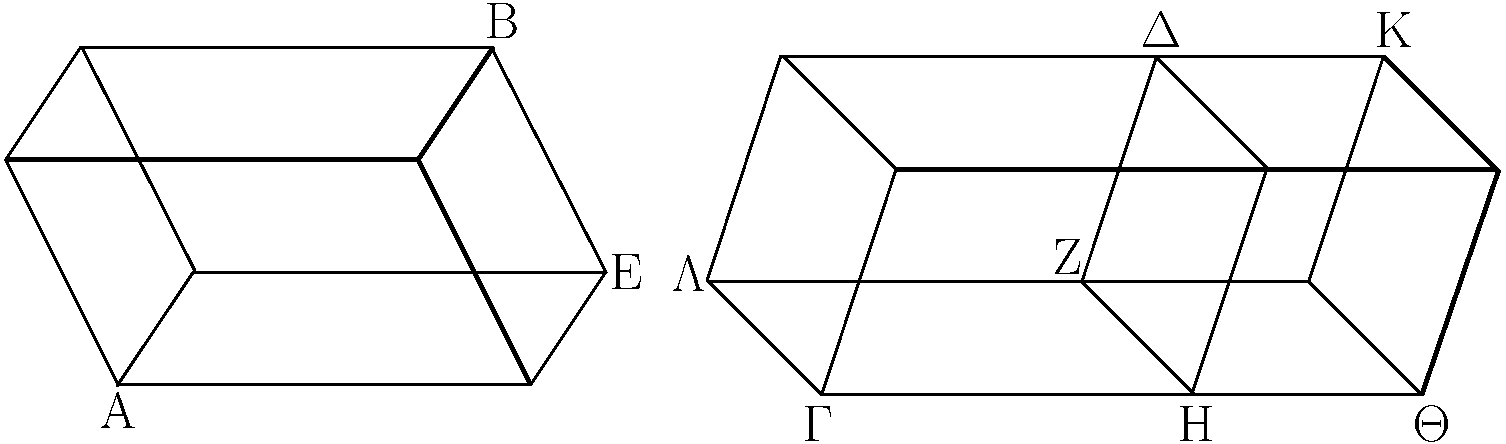
\includegraphics{Book11/fig32g.eps}}

\gr{>'Εστω ὑπὸ τὸ α\kern -.7pt  ὐτὸ <ύψοξ στερεὰ παραλληλεπίπεδα τὰ ΑΒ, ΓΔ;
λέγω, <ότι τὰ ΑΒ, ΓΔ στερεὰ παραλληλεπίπεδα πρὸξ >άλληλά ἐστιν
ὡξ αἱ βάσειξ, τουτέστιν <ότι ἐστὶν ὡξ ἡ ΑΕ βάσιξ πρὸξ τὴν
ΓΖ βάσιν, ο<ύτωξ τὸ ΑΒ στερεὸν πρὸξ τὸ ΓΔ στερεόν.}

\gr{Παραβεβλήσθω γὰρ παρὰ τὴν ΖΗ τῶ| ΑΕ >ίσον τὸ ΖJ, καὶ ἀπὸ βάσεωξ μὲν τῆξ ΖJ, <ύψουξ δὲ τοῦ α\kern -.7pt  ὐτοῦ τῶ| ΓΔ στερεὸν παραλληλεπίπεδον
συμπεπληρώσθω τὸ ΗΚ. >ίσον δή ἐστι τὸ ΑΒ στερεὸν τῶ| ΗΚ
στερεῶ|; ἐπί τε γὰρ >ίσων βάσεών εἰσι τῶν ΑΕ, ΖJ καὶ ὑπὸ τὸ
α\kern -.7pt  ὐτο <ύψοξ. καὶ ἐπεὶ στερεὸν παραλληλεπίπεδον τὸ ΓΚ ἐπιπέδῳ
τῶ| ΔΗ τέτμ\kern -.5pt  ηται παραλλήλῳ >όντι τοῖξ ἀπεναντίον ἐπιπέδοιξ,
>έστιν >άρα ὡξ ἡ ΓΖ βάσιξ πρὸξ τὴν ΖJ βάσιν, ο<ύτωξ τὸ ΓΔ
στερεὸν πρὸξ τὸ ΔJ στερεόν. >ίση δὲ ἡ μὲν ΖJ βάσιξ τῆ| ΑΕ
βάσει, τὸ δὲ ΗΚ στερεὸν τῶ| ΑΒ στερεῶ|; >έστιν >άρα καὶ ὡξ ἡ
ΑΕ βάσιξ πρὸξ τὴν ΓΖ βάσιν, ο<ύτωξ τὸ ΑΒ στερεὸν πρὸξ τὸ ΓΔ στερεόν.}

\gr{Τὰ >άρα ὑπὸ τὸ α\kern -.7pt  ὐτὸ <ύψοξ >όντα στερεὰ παραλληλεπίπεδα πρὸξ
>άλληλά ἐστιν ὡξ αἱ βάσειξ; <όπερ >έδει δεῖχαι.}}

\ParallelRText{
\begin{center}
{\large Proposition 32}
\end{center}

Parallelepiped solids which (have) the same height
are to one another as their bases.

\epsfysize=1.in
\centerline{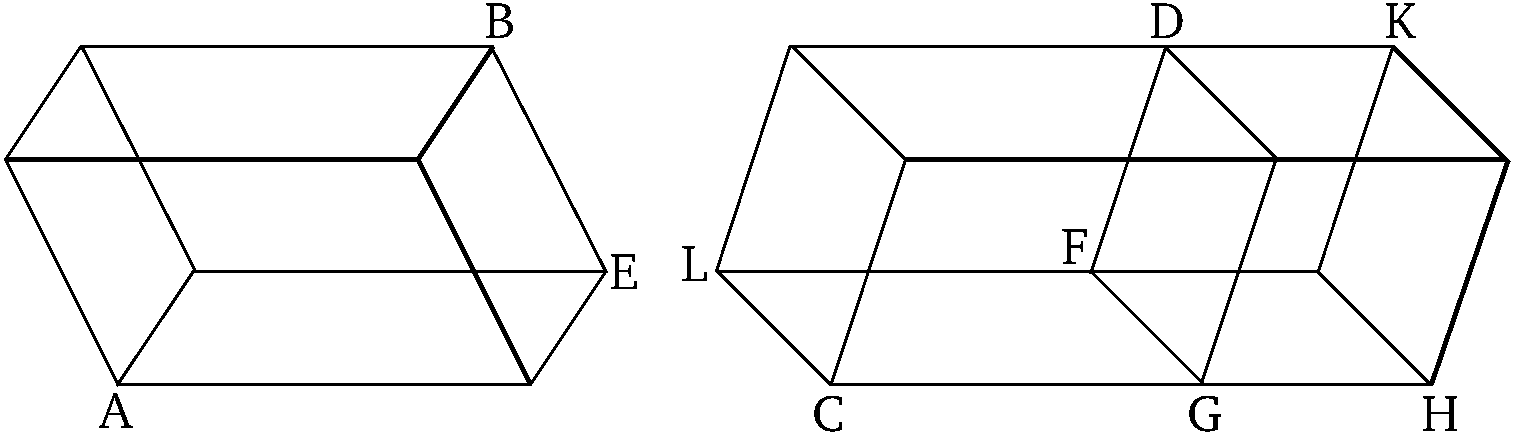
\includegraphics{Book11/fig32e.eps}}

Let $AB$ and $CD$ be parallelepiped solids (having) the same height.
I say that the parallelepiped solids $AB$ and $CD$
are to one another as their bases. That is to say, as base $AE$ is to base
$CF$, so solid $AB$ (is) to solid $CD$.

For let $FH$, equal to $AE$, be applied to $FG$ (in the angle
$FGH$ equal to angle $LCG$) [Prop.~1.45]. And let the parallelepiped solid $GK$, (having) the same height as $CD$, 
be completed on the base $FH$. So solid $AB$ is equal to solid
$GK$. For they are on the equal bases $AE$ and $FH$, and
(have) the same height [Prop.~11.31]. 
And since the parallelepiped solid $CK$ has been cut by the plane
$DG$, which is parallel to the opposite planes (of $CK$), thus as
the base $CF$ is to the base $FH$, so the solid $CD$ (is) to the
solid $DH$ [Prop.~11.25]. And  base
$FH$ (is) equal to base $AE$, and solid $GK$ to solid $AB$. And thus
as base $AE$ is to base $CF$, so solid $AB$ (is) to solid $CD$.

Thus, parallelepiped solids which (have) the same height
are to one another as their bases. (Which is) the very thing it was required to
show.}
\end{Parallel}

%%%%
%11.33
%%%%
\pdfbookmark[1]{Proposition 11.33}{pdf11.33}
\begin{Parallel}{}{}
\ParallelLText{
\begin{center}
{\large\ggn{33}.}
\end{center}\vspace*{-7pt}

\gr{Τὰ <όμοια στερεὰ παραλληλεπίπεδα πρὸξ >άλληλα ἐν τριπλασίονι
λόγῳ εἰσὶ τῶν ὁμολόγων πλευρῶν.}

\gr{>'Εστω <όμοια στερεὰ παραλληλεπίπεδα τὰ ΑΒ, ΓΔ, ὁμόλογοξ δὲ
>έστω ἡ ΑΕ τῆ| ΓΖ; λέγω, <ότι τὸ ΑΒ στερεὸν πρὸξ τὸ ΓΔ στερεὸν
τριπλασίονα λόγον >έθει, >ήπερ ἡ ΑΕ πρὸξ τὴν ΓΖ.}

\gr{Ἐκβεβλήσθωσαν γὰρ ἐπ> εὐθείαξ ταῖξ ΑΕ, ΗΕ, JΕ αἱ ΕΚ, ΕΛ, ΕΜ,
καὶ κείσθω τῆ| μὲν ΓΖ >ίση ἡ ΕΚ, τῆ| δὲ ΖΝ >ίση ἡ ΕΛ, καὶ
>έτι τῆ| ΖΡ >ίση ἡ ΕΜ, καὶ συμπεπληρώσθω τὸ ΚΛ παραλληλόγραμμον
καὶ τὸ ΚΟ στερεόν.}\\

\epsfysize=1.9in
\centerline{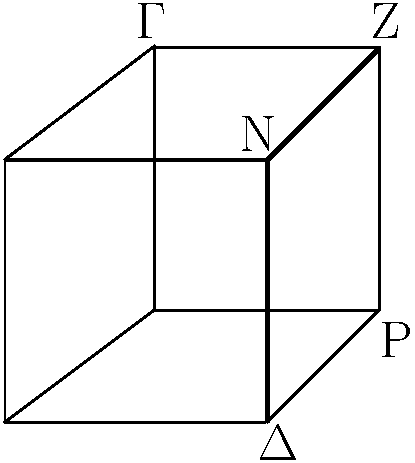
\includegraphics{Book11/fig33g.eps}}

\gr{Καὶ ἐπεὶ δύο αἱ ΚΕ, ΕΛ δυσὶ ταῖξ ΓΖ, ΖΝ >ίσαι εἰσίν, ἀλλὰ
καὶ γωνία ἡ ὑπὸ ΚΕΛ γωνίᾳ τῆ| ὑπὸ ΓΖΝ ἐστιν >ίση, ἐπειδήπερ
καὶ ἡ ὑπὸ ΑΕΗ τῆ| ὑπὸ ΓΖΝ ἐστιν >ίση διὰ τὴν ὁμοιότητα
τῶν ΑΒ, ΓΔ στερεῶν, >ίσον >άρα ἐστὶ [καὶ <όμοιον] τὸ ΚΛ
παραλληλόγραμμον τῶ| ΓΝ παραλληλογράμμῳ. διὰ τὰ α\kern -.7pt  ὐτὰ δὴ
καὶ τὸ μὲν ΚΜ παραλληλόγραμμον >ίσον ἐστὶ καὶ <όμοιον
τῶ| ΓΡ [παραλληλογράμμῳ] καὶ >έτι τὸ ΕΟ τῶ| ΔΖ; τρία >άρα παραλληλόγραμμα τοῦ ΚΟ στερεοῦ τρισὶ παραλληλογράμμοιξ τοῦ
ΓΔ στερεοῦ >ίσα ἐστὶ καὶ <όμοια. ἀλλὰ  τὰ μὲν τρία τρισὶ τοῖξ
ἀπεναντίον >ίσα ἐστὶ καὶ <όμοια, τὰ δὲ τρία τρισὶ τοῖξ
ἀπεναντίον >ίσα ἐστὶ καὶ <όμοια; <όλον >άρα τὸ ΚΟ στερεὸν
<όλῳ τῶ| ΓΔ στερεῶ| >ίσον ἐστὶ καὶ <όμοιον. συμπεπληρώσθω
τὸ ΗΚ παραλληλόγραμμον, καὶ ἀπὸ βάσεων μὲν τῶν ΗΚ, ΚΛ
παραλληλόγραμμων, <ύψουξ δὲ τοῦ α\kern -.7pt  ὐτοῦ τῶ| ΑΒ στερεὰ συμπεπληρώσθω τὰ ΕΧ, ΛΠ.  καὶ ἐπεὶ διὰ τὴν ὁμοιότητα τῶν
ΑΒ, ΓΔ στερεῶν ἐστιν ὡξ ἡ ΑΕ πρὸξ τὴν ΓΖ, ο<ύτωξ ἡ ΕΗ
πρὸξ τὴν ΖΝ, καὶ  ἡ ΕJ πρὸξ τὴν ΖΡ, >ίση δὲ ἡ μὲν ΓΖ τῆ|
ΕΚ, ἡ δὲ ΖΝ τῆ| ΕΛ, ἡ δὲ ΖΡ τῆ| ΕΜ, >έστιν >άρα ὡξ ἡ
ΑΕ πρὸξ τὴν ΕΚ, ο<ύτωξ ἡ ΗΕ πρὸξ τὴν ΕΛ καὶ ἡ JΕ πρὸξ
τὴν ΕΜ. ἀλλ> ὡξ μὲν ἡ ΑΕ πρὸξ τὴν ΕΚ, ο<ύτωξ τὸ ΑΗ
[παραλληλόγραμμον] πρὸξ τὸ ΗΚ παραλληλόγραμμον, ὡξ δὲ ἡ ΗΕ
πρὸξ τὴν ΕΛ, ο<ύτωξ τὸ ΗΚ πρὸξ τὸ ΚΛ,
ὡξ δὲ ἡ JΕ πρὸξ ΕΜ, ο<ύτωξ τὸ ΠΕ πρὸξ τὸ ΚΜ; καὶ ὡξ
>άρα τὸ ΑΗ παραλληλόγραμμον πρὸξ τὸ ΗΚ, ο<ύτωξ τὸ ΗΚ πρὸξ τὸ
ΚΛ καὶ τὸ ΠΕ πρὸξ τὸ ΚΜ. ἀλλ> ὡξ μὲν τὸ ΑΗ πρὸξ τὸ ΗΚ,
ο<ύτωξ τὸ ΑΒ στερεὸν πρὸξ τὸ ΕΧ στερεόν, ὡξ δὲ τὸ ΗΚ
πρὸξ τὸ ΚΛ, ο<ύτωξ τὸ ΧΕ στερεὸν πρὸξ τὸ ΠΛ στερεόν, ὡξ δὲ
τὸ ΠΕ πρὸξ τὸ ΚΜ, ο<ύτωξ τὸ ΠΛ στερεὸν πρὸξ τὸ ΚΟ στερεόν;
καὶ ὡξ >άρα τὸ ΑΒ στερεὸν πρὸξ τὸ ΕΧ, ο<ύτωξ τὸ ΕΧ πρὸξ τὸ 
ΠΛ καὶ τὸ ΠΛ πρὸξ τὸ ΚΟ. ἒαν δὲ τέσσαρα μεγέθη κατὰ τὸ
συνεθὲξ ἀνάλογον >ῆ|, τὸ πρῶτον πρὸξ τὸ τέταρτον τριπλασίονα λόγον
>έθει >ήπερ πρὸξ τὸ δεύτερον; τὸ ΑΒ >άρα στερεὸν πρὸξ τὸ ΚΟ
τριπλασίονα λόγον >έθει >ήπερ τὸ ΑΒ πρὸξ τὸ ΕΧ. ἀλλ> ὡξ τὸ
ΑΒ πρὸξ τὸ ΕΧ, ο<ύτωξ τὸ ΑΗ παραλληλόγραμμον πρὸξ τὸ ΗΚ
καὶ ἡ ΑΕ εὐθεῖα πρὸξ τὴν ΕΚ; <ώστε καὶ τὸ ΑΒ στερεὸν πρὸξ
τὸ ΚΟ  τριπλασίονα λόγον >έθει >ήπερ ἡ ΑΕ πρὸξ τὴν ΕΚ. >ίσον
δὲ τὸ [μὲν] ΚΟ στερεὸν τῶ| ΓΔ στερεῶ|, ἡ δὲ ΕΚ εὐθεῖα
τῆ| ΓΖ; καὶ τὸ ΑΒ >άρα στερεὸν πρὸξ τὸ ΓΔ στερεὸν τριπλασίονα
λόγον >έθει >ήπερ ἡ ὁμόλογοξ α\kern -.5pt  ὐτοῦ πλευρὰ ἡ ΑΕ πρὸξ
τὴν ὁμόλογον πλευρὰν τὴν ΓΖ.}

\epsfysize=2.5in
\centerline{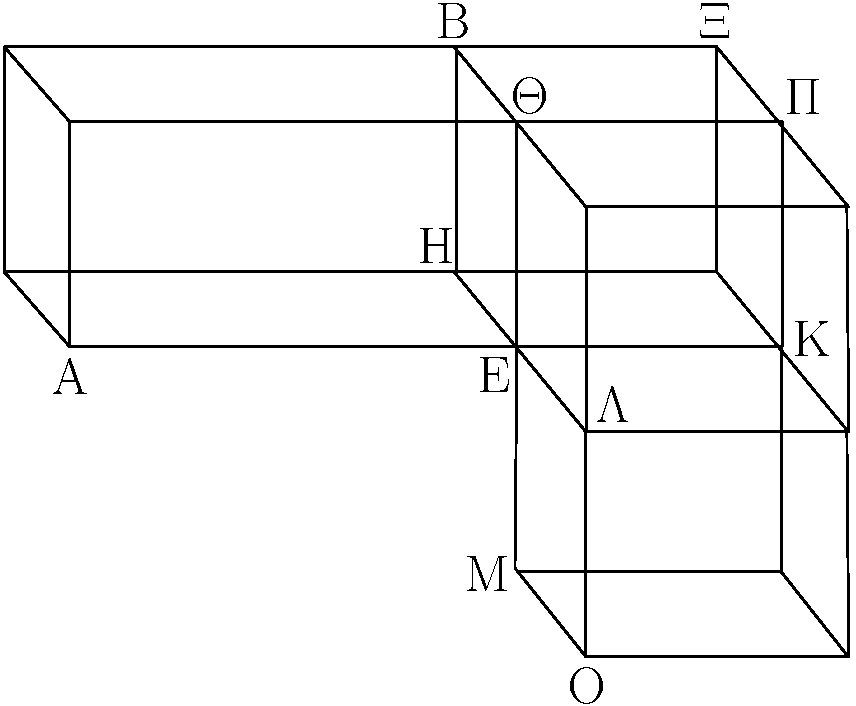
\includegraphics{Book11/fig33ag.eps}}

\gr{Τὰ >άρα <όμοια στερεὰ παραλληλεπίπεδα ἐν τριπλασίονι
λόγῳ ἐστὶ τῶν ὁμολόγων πλευρῶν; <όπερ >έδει
δεῖχαι.}}

\ParallelRText{

\begin{center}
{\large Proposition 33}
\end{center}

Similar parallelepiped solids are to one another
as the cubed ratio of their corresponding sides.

Let $AB$ and $CD$ be similar parallelepiped solids, and let $AE$
correspond to $CF$. I say that solid $AB$ has to solid $CD$ the
cubed ratio that $AE$ (has) to $CF$.

For let $EK$, $EL$, and $EM$ be produced in a straight-line
with $AE$, $GE$, and $HE$ (respectively). And let
$EK$ be made equal to $CF$, and $EL$ equal to $FN$, and, further,
$EM$ equal to $FR$. And let the parallelogram $KL$ be
completed, and the solid $KP$.\\

\epsfysize=1.9in
\centerline{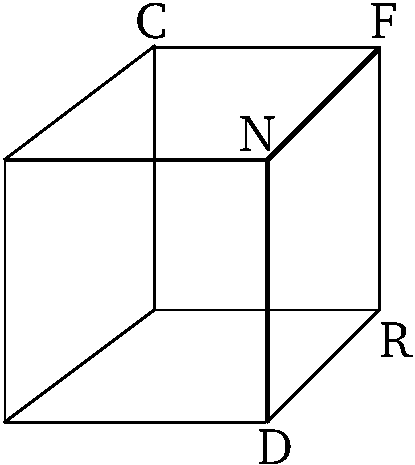
\includegraphics{Book11/fig33e.eps}}

And since the two (straight-lines) $KE$ and $EL$ are equal to the
two (straight-lines) $CF$ and $FN$, but angle $KEL$ is also
equal to angle $CFN$, inasmuch as $AEG$ is also equal to $CFN$,
on account of the similarity of the solids $AB$ and $CD$, parallelogram
$KL$ is thus equal [and similar] to parallelogram $CN$. So,
for the same (reasons), parallelogram $KM$ is also  equal and similar to
[parallelogram] $CR$, and, further, $EP$ to $DF$. Thus,
three parallelograms of solid $KP$ are equal and similar to three
parallelograms of solid $CD$. But the three (former parallelograms) are equal and
similar to the three opposite (parallelograms), and the three (latter parallelograms)
are equal and similar to the three opposite (parallelograms) 
[Prop.~11.24]. Thus, the whole of solid $KP$
is equal and similar to the whole of solid $CD$ [Def.~11.10]. Let parallelogram $GK$ be completed. And
let the the solids $EO$ and $LQ$, with bases the parallelograms
$GK$ and $KL$ (respectively), and with the same height as $AB$, be completed. And since, on account of the similarity of solids $AB$ and $CD$, 
as $AE$ is to $CF$, so $EG$ (is) to $FN$,  and $EH$  to $FR$ [Defs.~6.1, 11.9],
and $CF$ (is) equal to $EK$, and $FN$ to $EL$, and $FR$ to $EM$, 
thus as $AE$ is to $EK$, so $GE$ (is) to $EL$, and $HE$ to $EM$. But,
as $AE$ (is) to $EK$, so [parallelogram] $AG$ (is) to parallelogram
$GK$, and as $GE$ (is) to $EL$, so $GK$ (is) to $KL$,
and as $HE$ (is) to $EM$, so $QE$ (is) to $KM$ [Prop.~6.1]. And thus as parallelogram $AG$ (is) to $GK$, so $GK$
(is) to $KL$, and $QE$ (is) to $KM$. But, as $AG$
(is) to $GK$, so solid $AB$ (is) to solid $EO$, and as $GK$ (is) to $KL$,
so solid $OE$ (is) to  solid $QL$, and as $QE$ (is) to $KM$, so solid
$QL$ (is) to solid $KP$ [Prop.~11.32].
And, thus, as solid $AB$ is to $EO$, so $EO$ (is) to $QL$, and
$QL$ to $KP$.
And if four magnitudes are continuously proportional then the first has to
the fourth the cubed ratio that (it has) to the second [Def.~5.10].  Thus, solid $AB$ has to $KP$ the 
cubed ratio
which $AB$ (has) to $EO$. 
But, as $AB$ (is) to $EO$, so parallelogram $AG$
(is) to $GK$, and the straight-line $AE$ to $EK$ [Prop.~6.1]. Hence, 
solid $AB$ also has to $KP$ the cubed ratio  that $AE$ (has) to
$EK$. And solid $KP$ (is) equal to solid $CD$, and straight-line $EK$ to
$CF$.  Thus, solid $AB$ also has to solid $CD$ the cubed ratio
which its corresponding side $AE$ (has) to the corresponding side
$CF$.\\~\\

\epsfysize=2.5in
\centerline{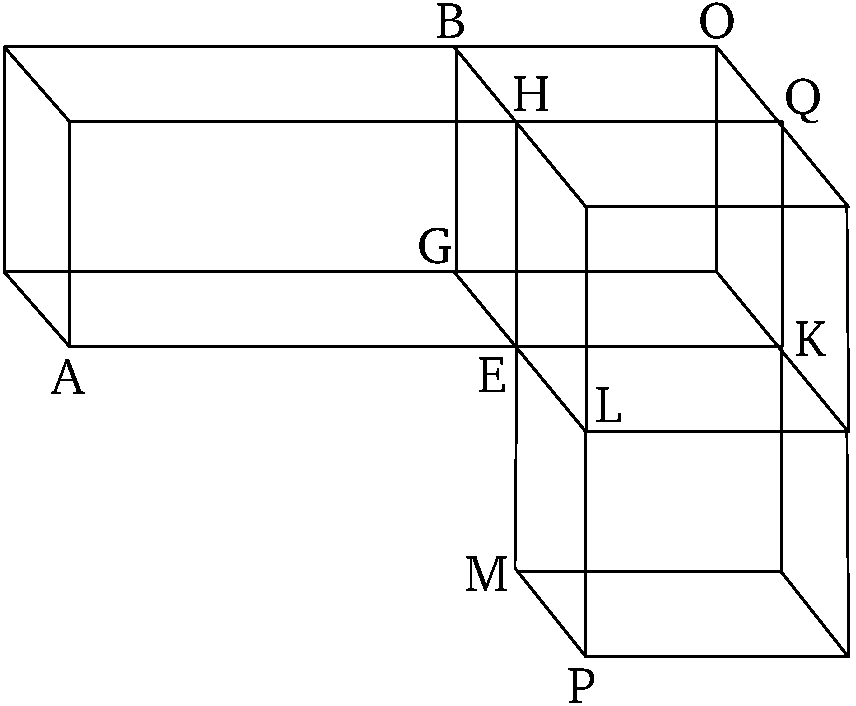
\includegraphics{Book11/fig33ae.eps}}

Thus, similar parallelepiped solids are to one another
as the cubed ratio of  their corresponding sides. (Which is) the very thing it
was required to show.}
\end{Parallel}

\begin{Parallel}{}{}
\ParallelLText{
\begin{center}
{\large \gr{Πόρισμα}.}
\end{center}\vspace*{-7pt}

\gr{Ἐκ δὴ τούτου φανερόν, <ότι ἒαν τέσσαρεξ εὐθεῖαι
ἀνάλογον >ῶσιν, >έσται ὡξ ἡ πρώτη πρὸξ τὴν τετάρτην, ο<ύτω
τὸ ἀπὸ τῆξ πρώτηξ στερεὸν παραλληλεπίπεδον πρὸξ τὸ ἀπὸ
τῆξ δευτέραξ τὸ <όμοιον καὶ ὁμοίωξ ἀναγραφόμενον, ἐπείπερ
καὶ ἡ πρώτη πρὸξ τὴν τετάρτην τριπλασίονα  λόγον >έθει
>ήπερ πρὸξ τὴν δευτέραν.}}

\ParallelRText{
\begin{center}
{\large Corollary}
\end{center}
So, (it is) clear, from this,  that if four straight-lines are (continuously)
proportional then as the first is to the fourth, so the parallelepiped
solid on the first will be to the similar, and similarly described, parallelepiped solid on the second, since the first also has to the fourth the
cubed ratio  that (it has) to the second.}
\end{Parallel}

%%%%
%11.34
%%%%
\pdfbookmark[1]{Proposition 11.34}{pdf11.34}
\begin{Parallel}{}{}
\ParallelLText{
\begin{center}
{\large \ggn{34}.}
\end{center}\vspace*{-7pt}

\gr{Τῶν >ίσων στερεῶν παραλληλεπιπέδων ἀντιπεπόνθασιν αἱ βάσειξ
τοῖξ <ύψεσιν; καὶ <ῶν στερεῶν παραλληλεπιπέδων ἀντιπεπόνθασιν
αἱ βάσειξ τοῖξ <ύψεσιν, <ίσα ἐστὶν ἐκεῖνα.}

\gr{>'Εστω >ίσα στερεὰ παραλληλεπίπεδα τὰ ΑΒ, ΓΔ; λέγω, <ότι
τῶν ΑΒ, ΓΔ στερεῶν παραλληλεπιπέδων ἀντιπεπόνθασιν αἱ βάσειξ
τοῖξ <ύψεσιν, καί ἐστιν ὡξ ἡ ΕJ βάσιξ πρὸξ τὴν ΝΠ βάσιν, ο<ύτωξ
τὸ τοῦ ΓΔ στερεοῦ <ύψοξ πρὸξ τὸ τοῦ ΑΒ στερεοῦ <ύψοξ.}

\gr{>'Εστωσαν γὰρ πρότερον αἱ ἐφεστηκυῖαι αἱ ΑΗ, ΕΖ, ΛΒ, JΚ,
ΓΜ, ΝΧ, ΟΔ, ΠΡ πρὸξ ὀρθὰξ ταῖξ βάσεσιν α\kern -.7pt  ὐτῶν; λέγω,
<ότι ἐστὶν ὡξ ἡ ΕJ βάσιξ πρὸξ τὴν ΝΠ βάσιν, ο<ύτωξ ἡ
ΓΜ πρὸξ τὴν ΑΗ.}

\gr{Εἰ μὲν ο>ῦν >ίση ἐστὶν ἡ ΕJ βάσιν τῆ| ΝΠ βάσει,
>έστι δὲ καὶ τὸ ΑΒ στερεὸν τῶ| ΓΔ στερεῶ| >ίσον, >έσται
καὶ ἡ ΓΜ τῆ| ΑΗ >ίση. τὰ γὰρ ὑπὸ τὸ α\kern -.7pt  ὐτὸ <ύψοξ στερεὰ
παραλληλεπίπεδα πρὸξ >άλληλά ἐστιν ὡξ αἱ βάσειξ. καὶ >έσται ὡξ ἡ ΕJ βάσιξ πρὸξ τὴν ΝΠ, ο<ύτωξ ἡ ΓΜ
πρὸξ τὴν ΑΗ, καὶ φανερόν, <ότι τῶν ΑΒ, ΓΔ στερεῶν παραλληλεπιπέδων
ἀντιπεπόνθασιν αἱ βάσειξ τοῖξ <ύψεσιν.}

\epsfysize=1.9in
\centerline{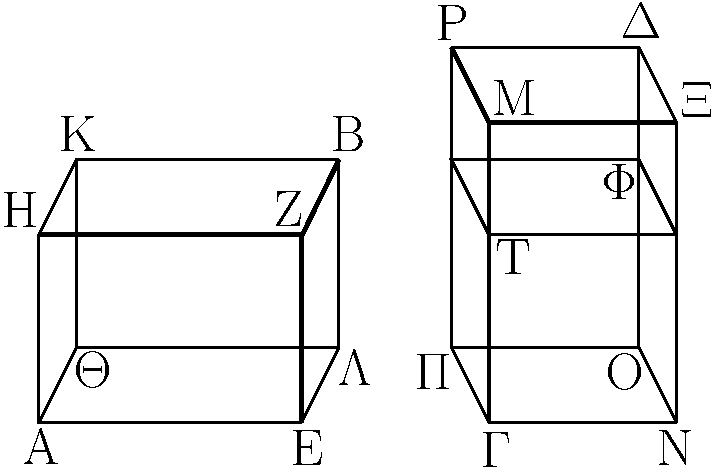
\includegraphics{Book11/fig34g.eps}}

\gr{μ\kern -.7pt  ὴ >έστω δὴ >ίση ἡ ΕJ βάσιξ τῆ| ΝΠ βάσει, ἀλλ> >έστω μείζων
ἡ ΕJ. >έστι δὲ καὶ τὸ ΑΒ στερεὸν τῶ| ΓΔ στερεῶ| >ίσον; μείζων >άρα
ἐστὶ καὶ ἡ ΓΜ τῆξ ΑΗ. κείσθω ο>ῦν τῆ| ΑΗ >ίση
ἡ ΓΤ, καὶ συμπεπληρώσθω ἀπὸ βάσεωξ μὲν τῆξ ΝΠ, <ύψουξ
δὲ τοῦ ΓΤ, στερεὸν παραλληλεπίπεδον τὸ ΦΓ. καὶ ἐπεὶ >ίσον
ἐστὶ τὸ ΑΒ στερεὸν τῶ| ΓΔ στερεῶ|, >έχωθεν δὲ τὸ ΓΦ, τὰ δὲ >ίσα
πρὸξ τὸ α\kern -.7pt  ὐτὸ τὸν α\kern -.5pt  ὐτὸν >έθει λόγον, >έστιν >άρα ὡξ τὸ 
ΑΒ στερεὸν πρὸξ τὸ
ΓΦ στερεόν, ο<ύτωξ τὸ ΓΔ στερεὸν πρὸξ τὸ ΓΦ στερεόν.
ἀλλ> ὡξ μὲν τὸ ΑΒ στερεὸν πρὸξ
 τὸ ΓΦ στερεόν, ο<ύτωξ
ἡ ΕJ βάσιξ πρὸξ τὴν ΝΠ βάσιν; ἰσο"υψῆ γὰρ τὰ ΑΒ, ΓΦ στερεά;
ὡξ δὲ τὸ ΓΔ στερεὸν πρὸξ τὸ ΓΦ στερεόν, ο<ύτωξ ἡ ΜΠ βάσιξ
πρὸξ τὴν ΤΠ βάσιν καὶ ἡ ΓΜ πρὸξ τὴν ΓΤ; καὶ ὡξ >άρα
ἡ ΕJ βάσιξ πρὸξ τὴν ΝΠ βάσιν, ο<ύτωξ ἡ ΜΓ πρὸξ τὴν ΓΤ.
>ίση δὲ ἡ ΓΤ τῆ| ΑΗ; καὶ ὡξ >άρα ἡ ΕJ βάσιξ πρὸξ τὴν ΝΠ
βάσιν, ο<ύτωξ ἡ ΜΓ πρὸξ τὴν ΑΗ. τῶν ΑΒ, ΓΔ >άρα στερεῶν
παραλληλεπιπέδων ἀντιπεπόνθασιν αἱ βάσειξ τοῖξ
<ύψεσιν.}

\gr{Πάλιν δὴ τῶν ΑΒ, ΓΔ στερεῶν παραλληλεπιπέδων ἀντιπεπονθέτωσαν
αἱ βάσειξ τοῖξ <ύψεσιν, καὶ >έστω ὡξ ἡ ΕJ βάσιξ πρὸξ τὴν ΝΠ
βάσιν, ο<ύτωξ τὸ τοῦ ΓΔ στερεοῦ <ύψοξ πρὸξ τὸ τοῦ ΑΒ στερεοῦ
<ύψοξ; λέγω, <ότι >ίσον ἐστὶ τὸ ΑΒ στερεὸν τῶ| ΓΔ στερεῶ|.}

\gr{>'Εστωσαν [γὰρ] πάλιν αἱ ἐφεστηκυῖαι πρὸξ ὀρθὰξ ταῖξ βάσεσιν.
καὶ εἰ μὲν >ίση ἐστὶν ἡ ΕJ βάσιξ τῆ| ΝΠ βάσει, καί ἐστιν ὡξ ἡ ΕJ
βάσιξ πρὸξ τὴν ΝΠ βάσιν, ο<ύτωξ τὸ τοῦ ΓΔ στερεοῦ <ύψοξ πρὸξ
τὸ τοῦ ΑΒ στερεοῦ <ύψοξ, >ίσον >άρα ἐστὶ καὶ τὸ τοῦ ΓΔ στερεοῦ
<ύψοξ τῶ| τοῦ ΑΒ στερεοῦ <ύψει. τὰ δὲ ἐπὶ >ίσων βάσεων στερεά
παραλληλεπίπεδα καὶ ὑπὸ τὸ α\kern -.7pt  ὐτὸ <ύψοξ >ίσα ἀλλήλοιξ ἐστίν;
>ίσον >άρα ἐστὶ τὸ ΑΒ στερεὸν τῶ|
ΓΔ στερεῶ|.}

\gr{μ\kern -.7pt  ὴ >έστω δὴ ἡ ΕJ βάσιξ τῆ| ΝΠ [βάσει] >ίση, ἀλλ> >έστω μείζων
ἡ ΕJ; μεῖζον >άρα ἐστὶ καὶ τὸ τοῦ ΓΔ στερεοῦ <ύψοξ τοῦ
τοῦ ΑΒ στερεοῦ <ύψουξ, τουτέστιν ἡ ΓΜ τῆξ ΑΗ. κείσθω τῆ|
ΑΗ >ίση πάλιν ἡ ΓΤ, καὶ συμπεπληρώσθω ὁμοίωξ τὸ ΓΦ στερεόν.
ἐπεί ἐστιν ὡξ ἡ ΕJ βάσιξ πρὸξ τὴν ΝΠ βάσιν, ο<ύτωξ
ἡ ΜΓ πρὸξ τὴν ΑΗ, >ίση δὲ ἡ ΑΗ τῆ| ΓΤ, >έστιν >άρα ὡξ ἡ ΕJ
βάσιξ πρὸξ τὴν ΝΠ βάσιν, ο<ύτωξ ἡ ΓΜ πρὸξ τὴν ΓΤ. ἀλλ>
ὡξ μὲν ἡ ΕJ [βάσιξ] πρὸξ τὴν ΝΠ βάσιν, ο<ύτωξ τὸ ΑΒ
στερεὸν πρὸξ τὸ ΓΦ στερεόν; ἰσο"υψῆ γάρ ἐστι τὰ ΑΒ, ΓΦ στερεά;
ὡξ δὲ ἡ ΓΜ πρὸξ τὴν ΓΤ, ο<ύτωξ <ή τε ΜΠ βάσιξ πρὸξ τὴν ΠΤ
βάσιν καὶ τὸ ΓΔ στερεὸν πρὸξ τὸ ΓΦ στερεόν. καὶ ὡξ >άρα τὸ ΑΒ
στερεὸν πρὸξ τὸ ΓΦ στερεόν, ο<ύτωξ τὸ ΓΔ στερεὸν πρὸξ τὸ ΓΦ
στερεόν; ἑκάτερον >άρα τῶν ΑΒ, ΓΔ πρὸξ τὸ ΓΦ τὸν α\kern -.7pt  ὐτὸν
>έθει λόγον. >ίσον >άρα ἐστὶ τὸ ΑΒ στερεὸν τῶ| ΓΔ στερεῶ|.}

\epsfysize=3in
\centerline{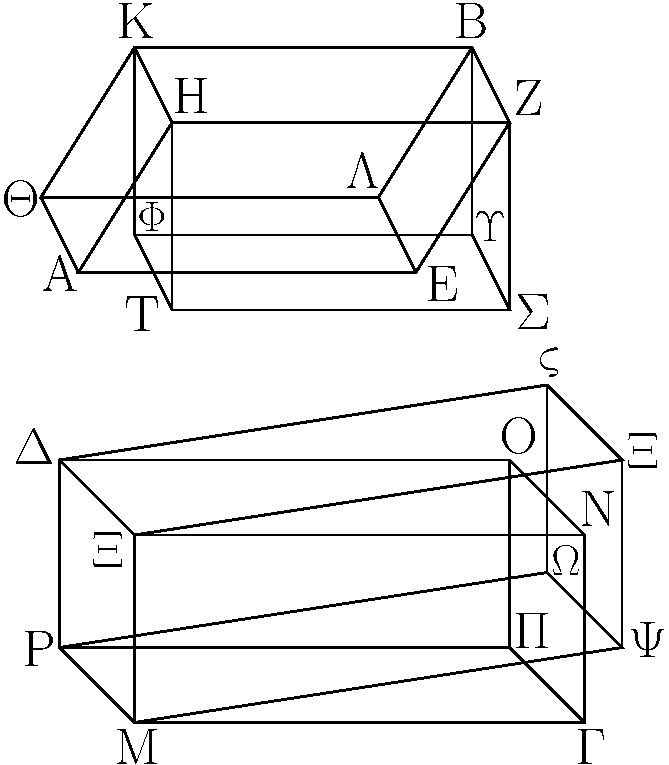
\includegraphics{Book11/fig34ag.eps}}

\gr{μ\kern -.7pt  ὴ >έστωσαν δὴ αἱ ἐφεστηκυῖαι αἱ ΖΕ, ΒΛ, ΗΑ, ΚJ, ΧΝ, ΔΟ, ΜΓ, ΡΠ
πρὸξ ὀρθὰξ ταῖξ βάσεσιν α\kern -.7pt  ὐτῶν, καὶ >ήθθωσαν ἀπὸ τῶν Ζ,
Η, Β, Κ, Χ, Μ, Ρ, Δ σημείων ἐπὶ τὰ διὰ τῶν ΕJ, ΝΠ ἐπίπεδα
κάθετοι καὶ συμβαλλέτωσαν τοῖξ ἐπιπέδοιξ κατὰ τὰ Σ, Τ, Υ, Φ,
Θ, Ψ, Ω, ξ, καὶ συμπεπληρώσθω τὰ ΖΦ, ΧΩ στερεά; λέγω, <ότι καὶ
ο<ύτωξ >ίσων >όντων τῶν ΑΒ, ΓΔ στερεῶν ἀντιπεπόνθασιν
αἱ βάσειξ τοῖξ <ύψεσιν, καί ἐστιν ὡξ ἡ ΕJ βἁσιν πρὸξ τὴν ΝΠ
βάσιν, ο<ύτωξ τὸ τοῦ ΓΔ στερεοῦ <ύψοξ πρὸξ τὸ τοῦ ΑΒ στερεοῦ
<ύψοξ.}

\gr{Ἐπεὶ >ίσον ἐστὶ τὸ ΑΒ στερεὸν τῶ| ΓΔ στερεῶ|, ἀλλὰ τὸ μὲν ΑΒ τῶ| ΒΤ ἐστιν >ίσον; ἐπί τε γὰρ τῆξ α\kern -.7pt  ὐτῆξ βάσεώξ εἰσι τῆξ
ΖΚ καὶ ὑπὸ τὸ α\kern -.7pt  ὐτὸ <ύψοξ;
τὸ δὲ ΓΔ στερεὸν τῶ| ΔΨ ἐστιν >ίσον; ἐπί τε γὰρ πάλιν τῆξ
α\kern -.5pt  ὐτῆξ βάσεώξ εἰσι τῆξ ΡΧ καὶ ὑπὸ τὸ α\kern -.3pt  ὐτὸ
<ύψοξ;
καὶ τὸ ΒΤ >άρα στερεὸν τῶ| ΔΨ στερεῶ| >ίσον ἐστίν.
>έστιν >άρα ὡξ ἡ ΖΚ βάσιξ πρὸξ τὴν ΧΡ βάσιν, ο<ύτωξ τὸ τοῦ
ΔΨ στερεοῦ <ύψοξ πρὸξ τὸ τοῦ ΒΤ στερεοῦ <ύψοξ. >ίση
δὲ ἡ μὲν ΖΚ βάσιξ τῆ| ΕJ βάσει, ἡ δὲ ΧΡ βάσιξ τῆ| ΝΠ βάσει; >έστιν
>άρα ὡξ ἡ ΕJ βάσιξ πρὸξ τὴν ΝΠ βάσιν, ο<ύτωξ τὸ τοῦ ΔΨ στερεοῦ
<ύψοξ πρὸξ τὸ τοῦ ΒΤ στερεοῦ <ύψοξ. τὰ δ> α\kern -.7pt  ὐτὰ <ύψη ἐστὶ τῶν
ΔΨ, ΒΤ στερεῶν καὶ τῶν ΔΓ, ΒΑ; >έστιν >άρα ὡξ ἡ ΕJ βάσιξ πρὸξ
τὴν ΝΠ βάσιν, ο<ύτωξ τὸ τοῦ ΔΓ στερεοῦ <ύψοξ πρὸξ τὸ τοῦ
ΑΒ στερεοῦ <ύψοξ. τῶν ΑΒ, ΓΔ >άρα στερεῶν παραλληλεπιπέδων
ἀντιπεπόνθασιν αἱ βάσειξ τοῖξ <ύψεσιν.}

\gr{Πάλιν δὴ τῶν ΑΒ, ΓΔ στερεῶν παραλληλεπιπέδων ἀντιπεπονθέτωσαν
αἱ βάσειξ τοῖξ <ύψεσιν, καὶ >έστω ὡξ ἡ ΕJ βάσιξ πρὸξ τὴν
ΝΠ βάσιν, ο<ύτωξ τὸ τοῦ ΓΔ στερεοῦ <ύψοξ πρὸξ τὸ τοῦ ΑΒ
στερεοῦ <ύψοξ; λέγω, <ότι >ίσον ἐστὶ τὸ ΑΒ στερεὸν τῶ| ΓΔ
στερεῶ|.}

\gr{Τῶν γὰρ α\kern -.7pt  ὐτῶν κατασκευασθέντων, ἐπεί ἐστιν ὡξ ἡ ΕJ βάσιξ
πρὸξ τὴν ΝΠ βάσιν, ο<ύτωξ τὸ τοῦ ΓΔ στερεοῦ <ύψοξ πρὸξ
τὸ τοῦ ΑΒ στερεοῦ <ύψοξ, >ίση δὲ ἡ μὲν ΕJ βάσιξ τῆ| ΖΚ βάσει,
ἡ δὲ ΝΠ τῆ| ΧΡ, >έστιν >άρα ὡξ ἡ ΖΚ βάσιξ πρὸξ τὴν ΧΡ βάσιν,
ο<ύτωξ τὸ τοῦ ΓΔ στερεοῦ <ύψοξ πρὸξ τὸ τοῦ ΑΒ στερεοῦ
<ύψοξ. τὰ δ> α\kern -.7pt  ὐτὰ <ύψη ἐστὶ τῶν ΑΒ, ΓΔ στερεῶν καὶ τῶν
ΒΤ, ΔΨ; >έστιν >άρα ὡξ ἡ ΖΚ βάσιξ πρὸξ τὴν ΧΡ βάσιν, ο<ύτωξ
τὸ τοῦ ΔΨ στερεοῦ <ύψοξ πρὸξ τὸ τοῦ ΒΤ στερεοῦ <ύψοξ. τῶν
ΒΤ, ΔΨ >άρα στερεῶν παραλληλεπιπέδων ἀντιπεπόνθασιν αἱ βάσειξ
τοῖξ <ύψεσιν; >ίσον
>άρα ἐστὶ τὸ ΒΤ στερεὸν τῶ| ΔΨ στερεῶ|. ἀλλὰ τὸ μὲν
ΒΤ τῶ| ΒΑ >ίσον ἐστίν; ἐπί τε γὰρ τῆξ α\kern -.5pt  ὐτῆξ βάσεωξ [εἰσι]
τῆξ ΖΚ καὶ ὑπὸ τὸ α\kern -.3pt  ὐτὸ <ύψοξ. τὸ δὲ ΔΨ στερεὸν τῶ|
ΔΓ στερεῶ| >ίσον ἐστίν. καὶ τὸ ΑΒ >άρα στερεὸν τῶ| ΓΔ στερεῶ|
ἐστιν >ίσον; <όπερ >έδει δεῖχαι.}}

\ParallelRText{
\begin{center}
{\large Proposition 34}$^\dag$
\end{center}

The  bases of equal parallelepiped solids are reciprocally proportional to their heights. And those parallelepiped solids
whose bases are reciprocally proportional to their heights are equal.

Let $AB$ and $CD$ be equal parallelepiped solids. I say that the
bases of the parallelepiped solids $AB$ and $CD$ are reciprocally
proportional to their heights, and (so) as base $EH$ is to base $NQ$, so the
height of solid $CD$ (is) to the height of solid $AB$.

For, first of all, let the (straight-lines) standing up, $AG$, $EF$, $LB$, $HK$, $CM$,
$NO$, $PD$, and $QR$,  be at right-angles to their bases. I say that
as base $EH$ is to base $NQ$, so $CM$ (is) to $AG$.

Therefore, if base $EH$ is equal to base $NQ$, and solid $AB$ is also
equal to solid $CD$, $CM$ will also be equal to $AG$. For
parallelepiped solids of the same height are to one another as their bases [Prop.~11.32]. And as base $EH$ (is) to $NQ$,
so $CM$ will be to $AG$. And (so it is) clear that the bases of the parallelepiped
solids $AB$ and $CD$ are reciprocally proportional to their heights.

\epsfysize=1.9in
\centerline{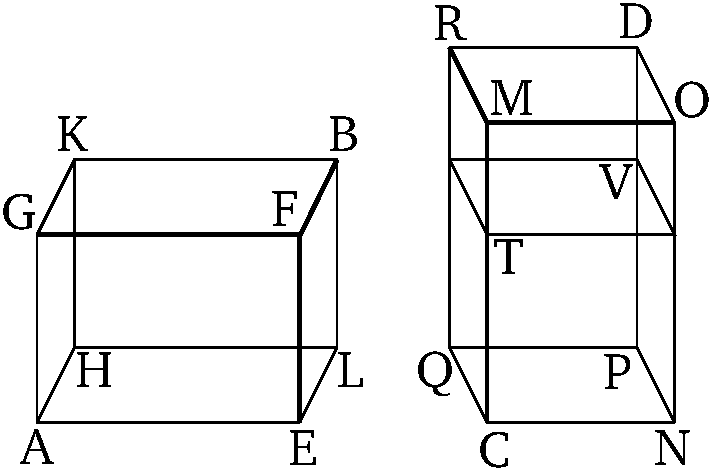
\includegraphics{Book11/fig34e.eps}}

So let base $EH$ not be equal to base $NQ$, but let $EH$ be greater. And
solid $AB$ is also equal to solid $CD$. Thus, $CM$ is also greater than $AG$.  Therefore, let $CT$ be made equal to $AG$. And let the parallelepiped
solid $VC$ be completed on the base $NQ$, with height $CT$.
And since solid $AB$ is equal to solid $CD$, and $CV$ (is)
extrinsic (to them), and equal (magnitudes) have the same ratio to the
same (magnitude) [Prop.~5.7], thus as solid
$AB$ is to solid $CV$, so solid $CD$ (is) to solid $CV$. But, as
solid $AB$ (is) to solid $CV$, so base $EH$ (is) to base $NQ$. For the solids $AB$ and $CV$ (are) of equal
height [Prop.~11.32]. And as solid $CD$ (is) to solid $CV$, so base $MQ$ (is) to 
base $TQ$ [Prop.~11.25], and $CM$ to $CT$
[Prop.~6.1].
And, thus, as base $EH$ is to base $NQ$, so $MC$ (is) to $AG$.
And $CT$ (is) equal to $AG$. And
thus as base $EH$ (is) to base $NQ$, so $MC$ (is) to $AG$. Thus, the
bases of the parallelepiped solids $AB$ and $CD$ are reciprocally proportional to their
heights.

So, again, let the bases of the parallelepipid solids $AB$ and $CD$
be reciprocally proportional to their heights, and let base $EH$
be to base $NQ$, as the height of solid $CD$ (is) to the
height of solid $AB$. I say that solid $AB$ is equal to solid $CD$.
\mbox{[}For] let the (straight-lines) standing up again be at right-angles to the
bases. And if base $EH$ is equal to base $NQ$, and as base $EH$
is to base $NQ$, so the height of solid $CD$ (is) to the
height of solid $AB$, the height of solid $CD$ is thus also
equal to the height of solid $AB$. And parallelepiped solids on equal
bases, and also with the same height,  are equal to one another [Prop.~11.31]. Thus, solid $AB$ is equal to solid $CD$.

So, let base $EH$ not be equal to [base] $NQ$, but let $EH$ be greater.
Thus, the height of solid $CD$ is also greater than the height of
solid $AB$, that is to say $CM$ (greater) than $AG$. Let $CT$ again
be made equal to $AG$, and let the solid $CV$ be similarly
completed.  Since as base $EH$ is to base $NQ$, so $MC$ (is) to
$AG$, and $AG$ (is) equal to $CT$, thus as base $EH$ (is) to
base $NQ$, so $CM$ (is) to $CT$.  But, as [base] $EH$ (is) to base
$NQ$, so solid $AB$ (is) to solid $CV$. For solids $AB$ and $CV$ are of equal heights [Prop.~11.32].
And as $CM$ (is) to $CT$, so (is) base $MQ$ to base $QT$ [Prop.~6.1], and solid $CD$ to solid $CV$ [Prop.~11.25]. And thus as solid $AB$ (is) to solid
$CV$, so solid $CD$ (is) to solid $CV$. Thus, $AB$ and $CD$ each
have the same ratio to $CV$. Thus, solid $AB$ is equal to solid
$CD$ [Prop.~5.9].\\~\\~\\~\\~\\

\epsfysize=3in
\centerline{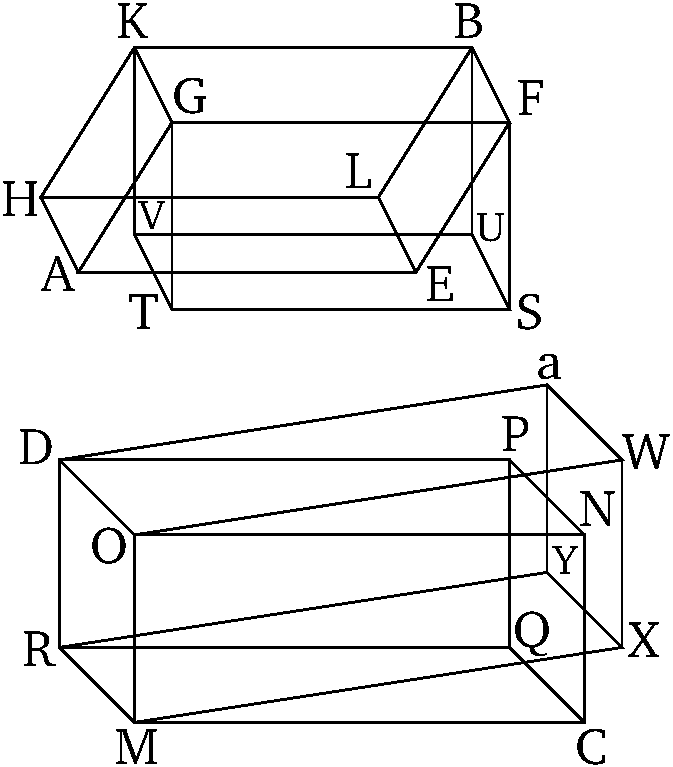
\includegraphics{Book11/fig34ae.eps}}

So, let the (straight-lines) standing up, $FE$, $BL$, $GA$, $KH$, $ON$,
$DP$, $MC$, and $RQ$, not be at right-angles to their bases.
And let perpendiculars be drawn to the planes through $EH$ and
$NQ$ from points $F$, $G$, $B$, $K$, $O$, $M$, $R$, and $D$, 
and let them have joined the planes at (points) $S$, $T$, $U$, $V$, $W$,
$X$, $Y$, and $a$ (respectively). And let the solids $FV$ and $OY$
be completed. In this case,  also, I say that the solids $AB$ and
$CD$ being equal, their bases are reciprocally proportional to their
heights, and (so) as base $EH$ is to base $NQ$, so the height of
solid $CD$ (is) to the height of solid $AB$.

Since solid $AB$ is equal to solid $CD$, but $AB$ is equal
to $BT$. For they are on the same base $FK$, and (have) the
same height [Props.~11.29, 11.30]. And solid $CD$ is equal is equal to $DX$. For, again,  they are on the same base $RO$, and (have) the same height [Props.~11.29, 11.30]. Solid
$BT$ is thus also equal to solid $DX$. Thus, as base $FK$ (is) to base $OR$,
so the height of solid $DX$ (is) to the height of solid $BT$ (see first part of 
proposition). And base
$FK$ (is) equal to base $EH$, and base $OR$ to $NQ$. Thus, as base
$EH$ is to base $NQ$, so the height of solid $DX$ (is) to the height
of solid $BT$. And solids $DX$, $BT$ are the same
height as (solids) $DC$,  $BA$ (respectively). Thus, as base $EH$
is to base $NQ$, so the height of solid $DC$ (is) to the height of solid
$AB$.  Thus, the bases of the parallelepiped solids $AB$ and $CD$
are reciprocally proportional to their heights.

So, again, let the bases of the parallelepiped solids $AB$ and $CD$ be
reciprocally proportional to their heights, and (so) let base $EH$ be to base $NQ$,
as the height of solid $CD$ (is) to the height of solid $AB$. I say
that solid $AB$ is equal to solid $CD$.

For, with the same construction (as before), since as base $EH$
is to base $NQ$, so the height of solid $CD$ (is) to the height
of solid $AB$, and base $EH$ (is) equal to base $FK$, and
$NQ$ to $OR$, thus as base $FK$ is to base $OR$, so the height
of solid $CD$ (is) to the height of solid $AB$. And solids $AB$, $CD$ are the same height as (solids) $BT$,  $DX$ (respectively). 
Thus, as base $FK$ is to base $OR$, so the height of solid $DX$ (is)
to the height of solid $BT$. Thus, the bases of the parallelepiped solids $BT$ and $DX$
are reciprocally proportional to their heights. Thus, solid $BT$ is equal to
solid $DX$ (see first part of  proposition). But, $BT$ is equal to $BA$. For [they are] on the same
base $FK$, and (have) the same height [Props.~11.29, 11.30]. And solid $DX$ is equal
to solid $DC$ [Props.~11.29, 11.30]. Thus, solid $AB$ is also equal to solid $CD$. (Which is) the very thing it was required to show.}
\end{Parallel}
{\footnotesize\noindent$^\dag$ This proposition assumes that (a) if
two parallelepipeds are equal, and have equal bases, then their heights are equal,
and (b) if the bases of two equal parallelepipeds are unequal, then that solid which
has the lesser base has the greater height.}

%%%%
%11.35
%%%%
\pdfbookmark[1]{Proposition 11.35}{pdf11.35}
\begin{Parallel}{}{}
\ParallelLText{
\begin{center}
{\large \ggn{35}.}
\end{center}\vspace*{-7pt}

\gr{Ἐὰν >ῶσι δύο γωνίαι ἐπίπεδοι >ίσαι, ἐπὶ δὲ τῶν
κορυφῶν α\kern -.7pt  ὐτῶν μετέωροι εὐθεῖαι ἐπισταθῶσιν
>ίσαξ γωνίαξ περιέθουσαι μετὰ τῶν ἐχ ἀρθῆξ
εὐθειῶν ἑκατέραν ἑκατέρᾳ, ἐπὶ δὲ τῶν μετεώρων
ληφθῆ| τυθόντα σημεῖα, καὶ ἀπ> α\kern -.7pt  ὐτῶν ἐπὶ τὰ ἐπίπεδα,
ἐν ο<ῖξ εἰσιν αἱ ἐχ ἀρθῆξ γωνίαι, κάθετοι ἀθθῶσιν,
ἀπὸ δὲ τῶν γενομένων σημείων ἐν τοῖξ ἐπιπέδοιξ
ἐπὶ τὰξ ἐχ ἀρθῆξ γωνίαξ ἐπιζευθθῶσιν εὐθεῖαι,
>ίσαξ γωνίαξ περιέχουσι μετὰ τῶν μετεώρων.}\\

\epsfysize=2.4in
\centerline{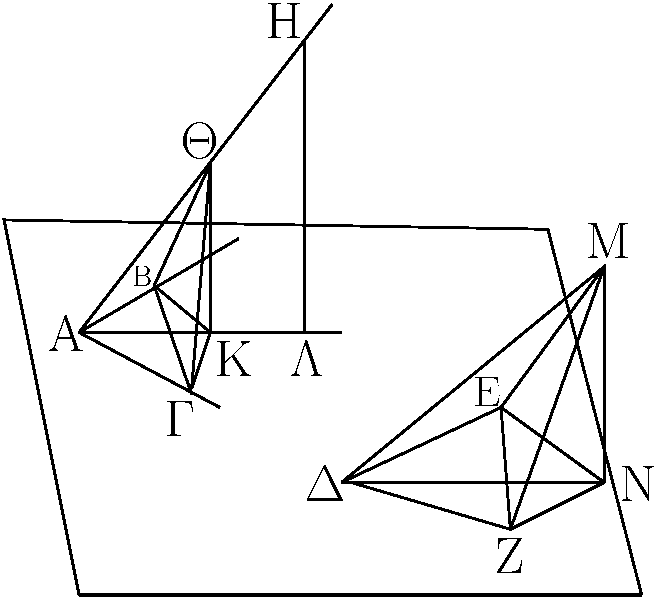
\includegraphics{Book11/fig35g.eps}}

\gr{>'Εστωσαν  δύο γωνίαι εὐθύγραμμοι >ίσαι αἱ ὑπὸ ΒΑΓ,
ΕΔΖ, ἀπὸ δὲ τῶν Α, Δ σημείων μετέωροι εὐθεῖαι ἐφεστάτ\-ωσαν
αἱ ΑΗ, ΔΜ >ίσαξ γωνίαξ περιέθουσιν μετὰ τῶν ἐχ ἀρθῆξ εὐθειῶν
ἑκατέραν ἑκατέρᾳ, τὴν μὲν ὑπὸ ΜΔΕ τῆ| ὑπὸ ΗΑΒ, τὴν δὲ
ὑπὸ ΜΔΖ τῆ| ὑπὸ ΗΑΓ, καὶ εἰλήφθω ἐπὶ τῶν ΑΗ, ΔΜ τυθόντα
σημεῖα τὰ Η, Μ, καὶ >ήθθωσαν ἀπὸ τῶν Η, Μ σημείων
ἐπὶ τὰ διὰ τῶν ΒΑΓ, ΕΔΖ ἐπίπεδα κάθετοι αἱ ΗΛ, ΜΝ, καὶ
συμβαλλέτωσαν τοῖξ ἐπιπέδοιξ κατὰ τὰ Λ, Ν,
καὶ ἐπεζεύθθωσαν αἱ ΛΑ, ΝΔ; λέγω, <ότι >ίση ἐστὶν ἡ ὑπὸ
ΗΑΛ γωνία τῆ| ὑπὸ ΜΔΝ γωνίᾳ.}

\gr{Κείσθω τῆ| ΔΜ >ίση ἡ ΑJ, καὶ >ήθθω διὰ τοῦ J σημείου τῆ|
ΗΛ παράλληλοξ ἡ JΚ. ἡ δὲ ΗΛ κάθετόξ ἐστιν ἐπὶ τὸ διὰ
τῶν ΒΑΓ ἐπίπεδον; καὶ ἡ JΚ >άρα κάθετόξ ἐστιν ἐπὶ
τὸ διὰ τῶν ΒΑΓ ἐπίπεδον. >ήθθωσαν ἀπὸ τῶν Κ, Ν
σημείων ἐπὶ τὰξ ΑΓ, ΔΖ, ΑΒ, ΔΕ εὐθείαξ κάθετοι αἱ ΚΓ, ΝΖ,
ΚΒ, ΝΕ, καὶ ἐπεζεύθθωσαν αἱ JΓ, ΓΒ, ΜΖ, ΖΕ. ἐπεὶ τὸ ἀπὸ
τῆξ JΑ >ίσον ἐστὶ τοῖξ ἀπὸ τῶν JΚ, ΚΑ, τῶ| δὲ ἀπὸ
τῆξ ΚΑ >ίσα ἐστὶ τὰ ἀπὸ τῶν ΚΓ, ΓΑ, καὶ τὸ ἀπὸ
τῆξ JΑ >άρα
 >ίσον ἐστὶ τοῖξ ἀπὸ τῶν  JΚ, ΚΓ, ΓΑ.
τοῖξ δὲ ἀπὸ τῶν JΚ, ΚΓ >ίσον ἐστὶ τὸ ἀπὸ τῆξ JΓ;
τὸ >άρα ἀπὸ τῆξ JΑ >ίσον ἐστὶ τοῖξ ἀπὸ τῶν
JΓ, ΓΑ. ὀρθὴ >άρα ἐστὶν ἡ ὑπὸ JΓΑ γωνία. διὰ τὰ α\kern -.7pt  ὐτὰ
δὴ καὶ ἡ ὑπὸ ΔΖΜ γωνία ὀρθή ἐστιν. >ίση >άρα ἐστὶν
ἡ ὑπὸ ΑΓJ γωνία τῆ| ὑπὸ ΔΖΜ. >έστι δὲ καὶ ἡ
ὑπὸ JΑΓ τῆ| ὑπὸ ΜΔΖ >ίση. δύο δὴ τρίγωνά ἐστι
τὰ ΜΔΖ, JΑΓ δύο γωνίαξ δυσὶ γωνίαιξ >ίσαξ >έθοντα
ἑκατέραν ἑκατέρᾳ καὶ μίαν πλευρὰν μιᾶ| πλευρᾶ|
>ίσην τὴν ὑποτείνουσαν ὑπὸ μίαν τῶν >ίσων γωνιῶν
τὴν JΑ τῆ| ΜΔ; καὶ τὰξ λοιπὰξ >άρα πλευρὰξ ταῖξ λοιπαῖξ
πλευραῖξ >ίσαξ <έχει ἑκατέραν ἑκαρέρᾳ. >ίση >άρα ἐστὶν
ἡ ΑΓ τῆ| ΔΖ. ὁμοίωξ δὴ δείχομεν, <ότι καὶ
ἡ ΑΒ τῆ| ΔΕ ἐστιν >ίση. ἐπεὶ ο>ῦν >ίση ἐστὶν ἡ
μὲν ΑΓ τῆ| ΔΖ, ἡ δὲ ΑΒ τῆ| ΔΕ, δύο δὴ αἱ ΓΑ, ΑΒ δυσὶ
ταῖξ
ΖΔ, ΔΕ >ίσαι εἰσίν. ἀλλὰ καὶ γωνία ἡ ὑπὸ
ΓΑΒ γωνίᾳ τῆ| ὑπὸ ΖΔΕ ἐστιν >ίση; βάσιξ >άρα ἡ ΒΓ βάσει
τῆ| ΕΖ  >ίση ἐστὶ καὶ τὸ τρίγωνον τῶ| τριγώνῳ καὶ αἱ λοιπαὶ
γωνίαι ταῖξ λοιπαῖξ γωνίαιξ;
>ίση >άρα ἡ ὑπὸ ΑΓΒ γωνία τῆ| ὑπὸ ΔΖΕ. >έστι δὲ
καὶ ὀρθὴ ἡ ὑπὸ ΑΓΚ ὀρθῆ| τῆ| ὑπὸ ΔΖΝ >ίση; καὶ
λοιπὴ >άρα ἡ ὑπὸ ΒΓΚ λοιπῆ| τῆ| ὑπὸ ΕΖΝ ἐστιν
>ίση. διὰ τὰ α\kern -.7pt  ὐτὰ δὴ καὶ ἡ ὑπὸ ΓΒΚ τῆ| ὑπὸ ΖΕΝ
ἐστιν >ίση.
δύο δὴ τρίγωνά ἐστι τὰ ΒΓΚ, ΕΖΝ
[τὰξ] δύο γωνίαξ δυσὶ γωνίαιξ >ίσαξ >έθοντα ἑκατέραν
ἑκατέρᾳ καὶ μίαν πλευρὰν μιᾶ| πλευρᾶ| >ίσην τὴν πρὸξ
ταῖξ >ίσαιξ γωνίαιξ τὴν ΒΓ τῆ| ΕΖ; καὶ τὰξ λοιπὰξ
>άρα πλευρὰξ ταῖξ λοιπαῖξ πλευραῖξ >ίσαξ <έχουσιν.
>ίση >άρα ἐστὶν ἡ ΓΚ τῆ| ΖΝ. >έστι δὲ καὶ ἡ ΑΓ τῆ|
ΔΖ >ίση; δύο δὴ αἱ ΑΓ, ΓΚ δυσὶ ταῖξ ΔΖ, ΖΝ >ίσαι
εἰσίν; καὶ ὀρθὰξ γωνίαξ περιέθουσιν. βάσιξ >άρα ἡ ΑΚ βάσει
τῆ| ΔΝ >ίση ἐστίν. καὶ ἐπεὶ >ίση ἐστὶν ἡ ΑJ τῆ|
ΔΜ, >ίσον ἐστὶ καὶ τὸ ἀπὸ τῆξ ΑJ τῶ| ἀπὸ
τῆξ ΔΜ. ἀλλὰ τῶ| μὲν ἀπὸ τῆξ ΑJ
 >ίσα ἐστὶ τὰ
ἀπὸ τῶν ΑΚ, ΚJ; ὀρθὴ γὰρ ἡ ὑπὸ ΑΚJ; τῶ| δὲ
ἀπὸ τῆξ ΔΜ >ίσα τὰ ἀπὸ τῶν ΔΝ, ΝΜ; ὀρθὴ γὰρ
ἡ ὑπὸ ΔΝΜ; τὰ >άρα ἀπὸ τῶν ΑΚ, ΚJ >ίσα
ἐστὶ τοῖξ ἀπὸ τῶν ΔΝ, ΝΜ, <ῶν τὸ ἀπὸ τῆξ ΑΚ
>ίσον ἐστὶ τῶ|  ἀπὸ τῆξ ΔΝ; λοιπὸν >άρα τὸ ἀπὸ
τῆξ ΚJ >ίσον ἐστὶ τῶ| ἀπὸ τῆξ ΝΜ; >ίση >άρα ἡ JΚ
τῆ| ΜΝ. καὶ ἐπεὶ δύο αἱ JΑ, ΑΚ δυσὶ ταῖξ ΜΔ, ΔΝ
>ίσαι εἰσὶν ἑκατέρα ἑκατέρᾳ, καὶ βάσιξ ἡ JΚ βάσει
τῆ| ΜΝ ἐδείθθη >ίση, γωνία >άρα ἡ ὑπὸ JΑΚ γωνίᾳ
τῆ| ὑπὸ ΜΔΝ ἐστιν >ίση.}

\gr{Ἐὰν >άρα >ῶσι δύο γωνίαι ἐπίπεδοι >ίσαι καὶ τὰ
ἑχῆξ τῆξ προτάσεωξ [<όπερ >έδει δεῖχαι].}}

\ParallelRText{
\begin{center}
{\large Proposition 35}
\end{center}

If there are two equal plane angles, and
raised straight-lines are stood on the apexes of them, containing equal angles respectively
with the original straight-lines (forming the angles), and random points are taken on the raised
(straight-lines), and perpendiculars are drawn from them to the planes
in which the original angles are, and straight-lines are joined  from the
points created in the planes to the (vertices of the) original angles, then they will enclose
equal angles with the raised (straight-lines).

\epsfysize=2.4in
\centerline{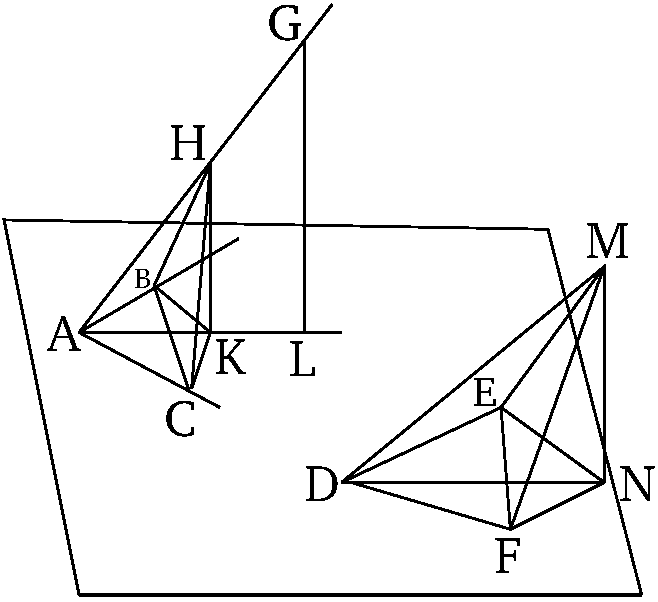
\includegraphics{Book11/fig35e.eps}}

Let $BAC$ and $EDF$ be two equal rectilinear angles. And let the raised
straight-lines $AG$ and $DM$ be stood  on points $A$ and $D$,
containing equal angles respectively with the original straight-lines. (That
is) $MDE$ (equal) to $GAB$, and $MDF$ (to) $GAC$. And let the random
points $G$ and $M$ be taken on $AG$ and $DM$ (respectively). 
And let the  $GL$ and $MN$ be drawn  from 
points $G$ and $M$ perpendicular to the planes through $BAC$ and $EDF$ (respectively).
And let them have joined the planes at points $L$ and $N$ (respectively).
And let $LA$ and $ND$ be joined. I say that angle $GAL$ is
equal to angle $MDN$.

Let $AH$ be made equal to $DM$. And let $HK$ be drawn through
point $H$ parallel to $GL$. And $GL$  is perpendicular to the plane
through $BAC$. Thus, $HK$  is also perpendicular to the plane through
$BAC$ [Prop.~11.8]. And let  $KC$, $NF$, $KB$, and $NE$ 
be drawn from points $K$ and $N$ perpendicular to the straight-lines $AC$, $DF$,
$AB$, and $DE$. And let $HC$, $CB$, $MF$, and $FE$ 
be joined. Since the (square) on $HA$ is equal to the (sum of the squares)
on $HK$ and $KA$ [Prop.~1.47], 
and the (sum of the squares) on $KC$ and $CA$ is equal to the (square) on $KA$   [Prop.~1.47], thus the  (square) on $HA$ is equal to the (sum
of the squares) on $HK$, $KC$, and $CA$. And the (square) on $HC$ is equal to the (sum of
the squares) on $HK$ and $KC$  [Prop.~1.47].
Thus, the (square) on $HA$ is equal to the (sum of the squares) on $HC$ and
$CA$. Thus, angle $HCA$ is a right-angle [Prop.~1.48]. So, for the same (reasons), angle $DFM$ is also
a right-angle. Thus, angle $ACH$ is equal to (angle) $DFM$. And $HAC$
is also equal to $MDF$.  So, $MDF$ and $HAC$
are two triangles
having two angles equal to two angles, respectively, and one side
equal to one side---(namely), that subtending one of the equal angles ---(that is), $HA$ (equal) to $MD$. 
Thus, they will also have the remaining sides equal to the remaining sides, respectively [Prop.~1.26]. Thus, $AC$ is equal to $DF$. So, similarly, we can show that $AB$ is also equal to $DE$. 
Therefore, since $AC$ is equal to $DF$, and $AB$ to $DE$, so the two
(straight-lines) $CA$ and $AB$ are equal to the two (straight-lines)
$FD$ and $DE$ (respectively). But, angle
$CAB$ is also equal to angle $FDE$. Thus, base $BC$ is equal to base
$EF$, and triangle ($ACB$) to triangle ($DFE$), and the remaining angles
to the remaining angles (respectively) [Prop.~1.4].
Thus, angle  $ACB$ (is) equal to $DFE$. And the right-angle $ACK$
is also equal to the right-angle $DFN$. Thus, the remainder
$BCK$ is equal to the remainder $EFN$. So, for the same (reasons), 
$CBK$ is also equal to $FEN$. So, $BCK$ and $EFN$
are two triangles having two angles equal to two angles, respectively, 
and one side equal to one side---(namely), that by the equal angles---(that is), $BC$ (equal) to $EF$. Thus, they will also have the remaining
sides equal to the remaining sides (respectively) [Prop.~1.26]. Thus, $CK$ is equal to $FN$. And $AC$ (is) also
equal to $DF$. So, the two (straight-lines) $AC$ and $CK$
are equal to the two (straight-lines) $DF$ and $FN$ (respectively). 
And they enclose right-angles. Thus, base $AK$ is equal to base $DN$
[Prop.~1.4]. 
And since $AH$ is equal to $DM$, the (square) on $AH$ is also equal
to the (square) on $DM$. But, the the (sum of the squares) on $AK$ and $KH$ is equal to the (square) on $AH$. For angle $AKH$
(is) a right-angle [Prop.~1.47]. And the (sum of the 
squares) on $DN$ and
$NM$ (is) equal to the square
on $DM$. For angle $DNM$ (is) a right-angle [Prop.~1.47]. Thus, the (sum of the squares) on $AK$ and
$KH$ is equal to the (sum of the squares) on $DN$ and $NM$, of
which the (square) on $AK$ is equal to the (square) on $DN$. Thus, the
remaining (square) on $KH$ is equal to the (square) on $NM$. Thus,
$HK$ (is) equal to $MN$. And since the two (straight-lines) $HA$ and
$AK$ are equal to the two (straight-lines) $MD$ and $DN$, respectively,
and base $HK$ was shown (to be) equal to base $MN$,  angle
$HAK$ is thus equal to angle $MDN$ [Prop.~1.8].

Thus, if there are two equal plane angles, and so on of the proposition. [(Which is) the very thing it was required to show].}
\end{Parallel}

\begin{Parallel}{}{}
\ParallelLText{
\begin{center}
{\large \gr{Πόρισμα}.}
\end{center}\vspace*{-7pt}

\gr{Ἐκ δὴ τούτου φανερόν, <ότι, ἓαν >ῶσι δύο γωνίαι ἐπίπεδοι
>ίσαι, ἐπισταθῶσι δὲ ἐπ> α\kern -.7pt  ὐτῶν μετέωροι εὐθεῖαι >ίσαι
>ίσαξ γωνίαξ περιέθουσαι μετὰ τῶν ἐχ ἀρθῆξ εὐθειῶν
ἑκατέραν ἑκατέρᾳ, αἱ ἀπ> α\kern -.7pt  ὐτῶν κάθετοι
ἀγόμεναι ἐπὶ τὰ ἐπίπεδα, ἐν ο<ῖξ εἰσιν αἱ ἐχ ἀρθῆξ
γωνίαι, >ίσαι ἀλλήλαιξ εἰσίν. <όπερ >έδει δεῖχαι.}}

\ParallelRText{
\begin{center}
{\large Corollary}
\end{center}

So,  it is clear, from this, that if there are two equal plane angles,
and equal raised straight-lines are stood on them (at their apexes), containing equal
angles respectively with the original straight-lines (forming the angles), then the perpendiculars
drawn from (the raised ends of) them to the planes in which the original angles lie are equal
to one another. (Which is) the very thing it was required to show.}
\end{Parallel}

%%%%
%11.36
%%%%
\pdfbookmark[1]{Proposition 11.36}{pdf11.36}
\begin{Parallel}{}{}
\ParallelLText{
\begin{center}
{\large \ggn{36}.}
\end{center}\vspace*{-7pt}

\gr{Ἐὰν τρεῖξ εὐθεῖαι ἀνάλογον >ῶσιν, τὸ ἐκ τῶν τριῶν
στερεὸν παραλληλεπίπεδον >ίσον ἐστὶ τῶ| ἀπὸ τῆξ μέσηξ
στερεῶ| παραλληλεπιπέδῳ ἰσοπλεύρῳ μέν, ἰσογωνίῳ δὲ τῶ|
προειρημένῳ.}\\~\\

\epsfysize=1.8in
\centerline{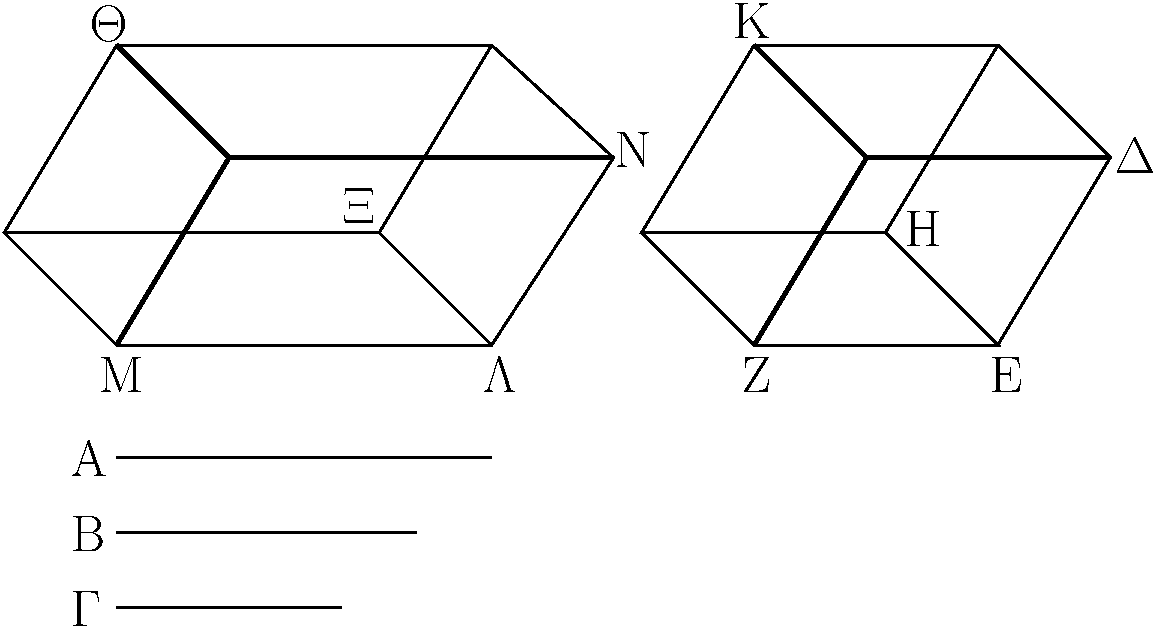
\includegraphics{Book11/fig36g.eps}}

\gr{>'Εστωσαν τρεῖξ εὐθεῖαι ἀνάλογον αἱ Α, Β, Γ, ὡξ ἡ Α πρὸξ τὴν
Β, ο<ύτωξ ἡ Β πρὸξ τὴν Γ; λέγω, <ότι τὸ ἐκ τῶν Α, Β, Γ
στερεὸν >ίσον ἐστὶ τῶ| ἀπὸ τῆξ Β στερεῶ| ἰσοπλεύρῳ μέν,
ἰσογωνίῳ δὲ τῶ| προειρημένῳ.}

\gr{Ἐκκείσθω στερεὰ γωνία ἡ πρὸξ τῶ| Ε περιεθομένη ὑπὸ τῶν
ὑπὸ ΔΕΗ, ΗΕΖ, ΖΕΔ, καὶ κείσθω τῆ| μὲν Β >ίση ἑκάστη τῶν
ΔΕ, ΗΕ, ΕΖ, καὶ συμπεπληρώσθω τὸ ΕΚ στερεὸν παραλληλεπίπεδον,
τῆ| δὲ Α >ίση ἡ ΛΜ, καὶ συνεστάτω πρὸξ τῆ| ΛΜ εὐθείᾳ
καὶ τῶ| πρὸξ α\kern -.7pt  ὐτῆ| σημείῳ τῶ| Λ τῆ| πρὸξ τῶ| Ε στερεᾶ|
γωνίᾳ >ίση στερεὰ γωνία ἡ περειθομένη ὑπὸ τῶν ΝΛΧ,
ΧΛΜ, ΜΛΝ, καὶ κείσθω τῆ| μὲν Β >ίση ἡ ΛΧ, τῆ| δὲ Γ
>ίση ἡ ΛΝ. καὶ ἐπεί ἐστιν ὡξ ἡ Α πρὸξ τὴν Β, ο<ύτωξ
ἡ Β πρὸξ τὴν Γ, >ίση δὲ ἡ μὲν Α τῆ| ΛΜ, ἡ δὲ Β ἑκατέρᾳ τῶν
ΛΧ, ΕΔ, ἡ δὲ Γ τῆ| ΛΝ, >έστιν >άρα ὡξ ἡ ΛΜ πρὸξ τὴν ΕΖ,
ο<ύτωξ ἡ ΔΕ πρὸξ τὴν ΛΝ. καὶ περὶ >ίσαξ γωνίαξ τὰξ ὑπὸ
ΝΛΜ, ΔΕΖ αἱ πλευραὶ ἀντιπεπόνθασιν; >ίσον >άρα ἐστὶ τὸ ΜΝ
παραλληλόγραμμον τῶ| ΔΖ παραλληλογραμάμμῳ. καὶ ἐπεὶ δύο
γωνίαι ἐπίπεδοι εὐθύγραμμοι >ίσαι εἰσὶν αἱ ὑπὸ ΔΕΖ, ΝΛΜ,
καὶ ἐπ> α\kern -.7pt  ὐτῶν μετέωροι εὐθεῖαι ἐφεστᾶσιν  αἱ ΛΧ, ΕΗ
>ίσαι τε ἀλλήλαιξ καὶ >ίσαξ γωνίαξ περιέθουσαι μετὰ τῶν ἐχ
ἀρθῆξ εὐθειῶν ἑκατέραν ἑκατέρᾳ, αἱ >άρα ἀπὸ τῶν
Η, Χ σημείων κάθετοι ἀγόμεναι ἐπὶ τὰ διὰ τῶν ΝΛΜ, ΔΕΖ
ἐπίπεδα >ίσαι ἀλλήλαιξ εἰσίν; <ώστε τὰ ΛJ, ΕΚ στερεὰ ὑπὸ
τὸ α\kern -.5pt  ὐτὸ <ύψοξ ἐστίν. τὰ δὲ ἐπὶ >ίσων βάσεων στερεὰ παραλληλεπίπεδα καὶ ὑπὸ τὸ α\kern -.3pt  ὐτὸ <ύψοξ >ίσα ἀλλήλοιξ ἐστίν; >ίσον >άρα ἐστὶ τὸ
JΛ στερεὸν τῶ| ΕΚ στερεῶ|. καί ἐστι τὸ μὲν ΛJ τὸ ἐκ τῶν Α, Β, Γ
στερεόν, τὸ δὲ ΕΚ τὸ ἀπὸ τῆξ Β στερεόν; τὸ >άρα ἐκ τῶν Α, Β, Γ
στερεὸν παραλληλεπίπεδον >ίσον ἐστὶ τῶ| ἀπὸ τῆξ Β στερεῶ|
ἰσοπλεύρῳ μέν, ἰσογωνίῳ δὲ τῶ| προειρημένῳ; <όπερ
>έδει δεῖχαι.}}

\ParallelRText{
\begin{center}
{\large Proposition 36}
\end{center}

If three straight-lines are (continuously)
proportional then the parallelepiped solid (formed) from the three (straight-lines) is equal
to the equilateral parallelepiped solid on the middle (straight-line which is)
equiangular to the aforementioned (parallelepiped solid).

\epsfysize=1.8in
\centerline{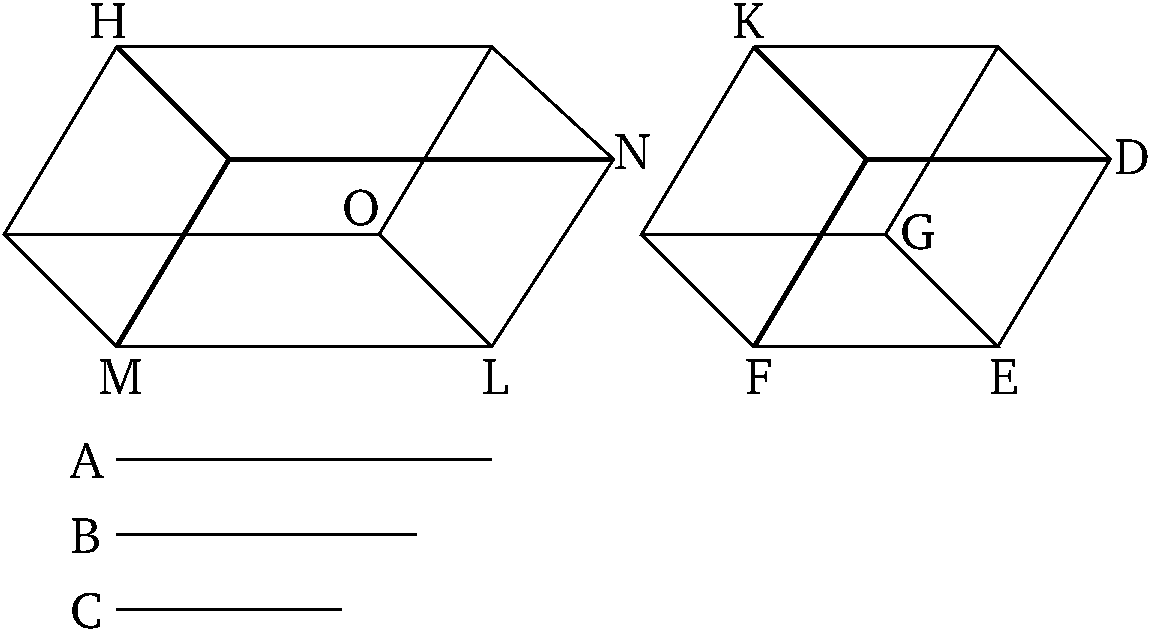
\includegraphics{Book11/fig36e.eps}}

Let $A$, $B$, and $C$ be three (continuously) proportional straight-lines,
(such that) as $A$ (is) to $B$, so $B$ (is) to $C$. I say that
the (parallelepiped) solid (formed) from $A$, $B$, and $C$ is
equal to the equilateral solid on $B$ (which is) equiangular with the
aforementioned (solid).

Let the solid angle at $E$, contained by $DEG$, $GEF$, and
$FED$, be set out. And let $DE$, $GE$, and $EF$ each be made equal
to $B$. And let the parallelepiped solid $EK$ be completed.
And (let) $LM$ (be made) equal to $A$. And let the solid angle
contained by $NLO$, $OLM$, and $MLN$ be constructed
on the straight-line $LM$, and at the point $L$ on it, (so as to be)
equal to the solid angle $E$ [Prop.~11.23]. 
And let $LO$ be made equal to $B$, and $LN$ equal  to $C$. And
since as $A$ (is) to $B$, so $B$ (is) to $C$, and $A$ (is) equal to
$LM$, and $B$ to each of $LO$ and $ED$, and $C$ to $LN$,
thus as $LM$ (is) to $EF$, so $DE$ (is) to $LN$. And (so) the sides
around the equal angles $NLM$ and $DEF$ are reciprocally
proportional. Thus, parallelogram $MN$ is equal to parallelogram
$DF$ [Prop.~6.14]. And since the
two plane rectilinear angles $DEF$ and $NLM$ are equal, and the raised straight-lines
stood on them (at their apexes), $LO$ and $EG$, are equal to one another,
and contain equal angles respectively with the original straight-lines (forming the angles),  the perpendiculars drawn from points $G$ and $O$
to the planes through $NLM$ and $DEF$ (respectively) are thus
equal to one another [Prop.~11.35~corr.]. 
Thus, the solids $LH$ and $EK$ (have) the same height. And
parallelepiped solids on equal bases, and with the same height, are
equal to one another [Prop.~11.31]. Thus,
solid $HL$ is equal to solid $EK$. And $LH$ is the solid (formed)
from $A$, $B$, and $C$, and $EK$ the solid on $B$. Thus,
the parallelepiped solid (formed) from $A$, $B$, and $C$ is equal
to the equilateral solid on $B$ (which is) equiangular with the
aforementioned (solid). (Which is) the very thing it was required to show.}
\end{Parallel}

%%%%
%11.37
%%%%
\pdfbookmark[1]{Proposition 11.37}{pdf11.37}
\begin{Parallel}{}{}
\ParallelLText{
\begin{center}
{\large \ggn{37}.}
\end{center}\vspace*{-7pt}

\gr{Ἐὰν τέσσαρεξ εὐθεῖαι ἀνάλογον >ῶσιν, καὶ τὰ ἀπ> α\kern -.7pt  ὐτῶν
στερεὰ παραλληλεπίπεδα <όμοιά τε καὶ ὁμοίωξ ἀναγραφόμενα ἀνάλογον
>έσται; καὶ ἒαν τὰ ἀπ> α\kern -.7pt  ὐτῶν στερεὰ παραλληλεπίπεδα <όμοιά
τε καὶ ὁμοίωξ ἀναγραφόμενα ἀνάλογον >ῆ|, καὶ α\kern -.5pt  ὐταὶ αἱ εὐθεῖαι
ἀνάλογον >έσονται.}\\

\epsfysize=1.9in
\centerline{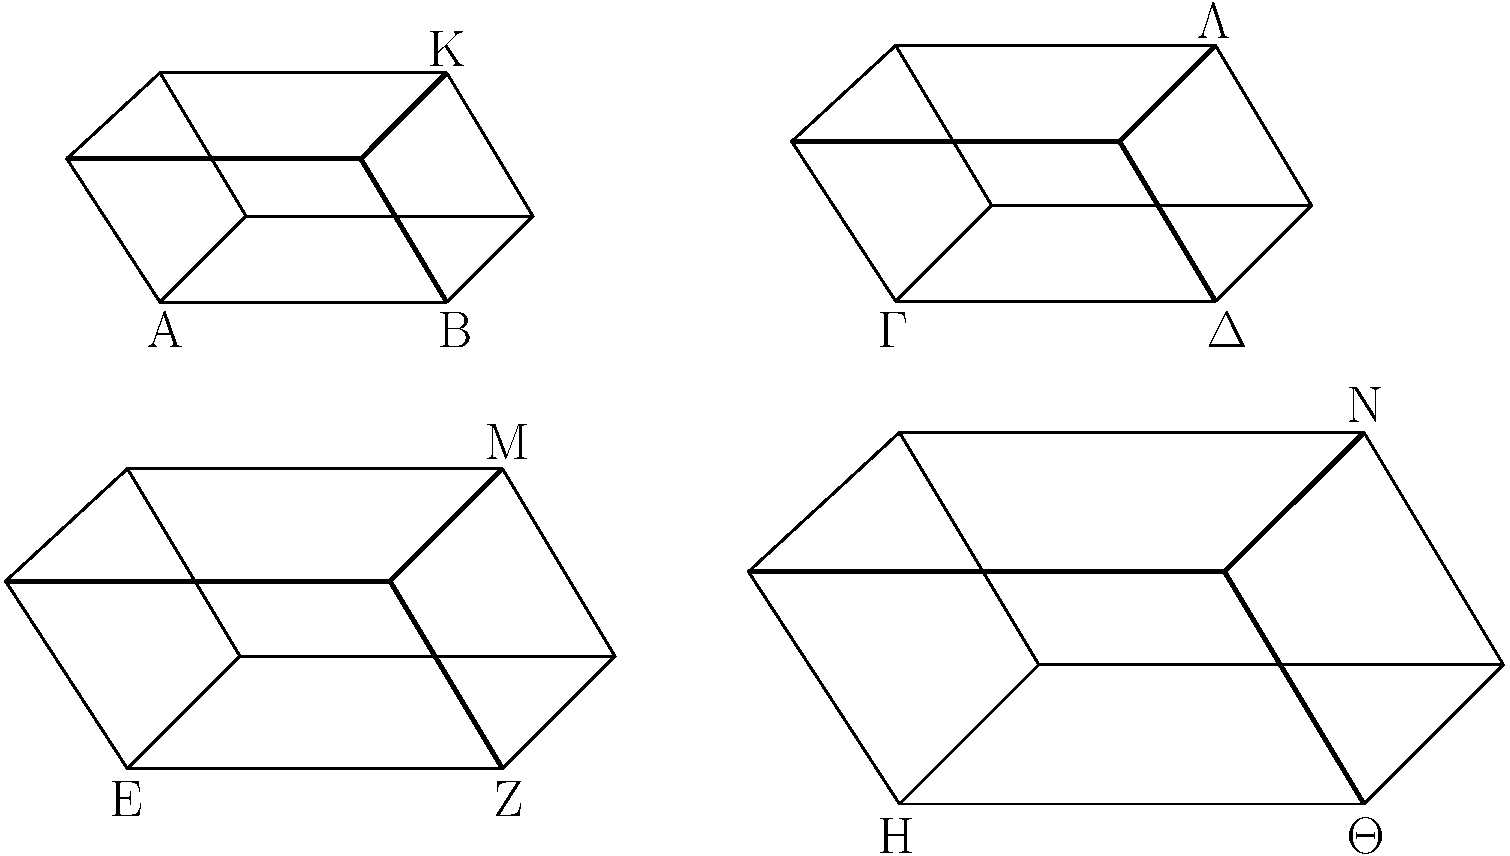
\includegraphics{Book11/fig37g.eps}}

\gr{>'Εστωσαν τέσσαρεξ εὐθεῖαι ἀνάλογον αἱ ΑΒ, ΓΔ, ΕΖ, ΗJ, ὡξ ἡ ΑΒ
πρὸξ τὴν ΓΔ, ο<ύτωξ ἡ ΕΖ πρὸξ τὴν ΗJ, καὶ ἀναγεγράφθωσαν
ἀπὸ τῶν ΑΒ, ΓΔ, ΕΖ, ΗJ <όμοιά τε καὶ ὁμοίωξ κείμενα στερεὰ
παραλληλεπίπεδα τὰ ΚΑ, ΛΓ, ΜΕ, ΝΗ; λέγω, <ότι ἐστὶν ὡξ τὸ ΚΑ
πρὸξ τὸ ΛΓ, ο<ύτωξ τὸ ΜΕ πρὸξ τὸ ΝΗ.}

\gr{Ἐπεὶ γὰρ <όμοιόν ἐστι τὸ ΚΑ στερεὸν παραλληλεπίπεδον τῶ|
ΛΓ, τὸ ΚΑ >άρα πρὸξ τὸ ΛΓ τριπλασίονα λόγον >έθει >ήπερ
ἡ ΑΒ πρὸξ τὴν ΓΔ. διὰ τὰ α\kern -.7pt  ὐτὰ δὴ καὶ τὸ ΜΕ πρὸξ τὸ ΝΗ τριπλασίονα
λόγον >έθει >ήπερ ἡ ΕΖ πρὸξ τὴν ΗJ. καί ἐστιν ὡξ ἡ ΑΒ πρὸξ
τὴν ΓΔ, ο<ύτωξ ἡ ΕΖ πρὸξ τὴν ΗJ. καὶ ὡξ
>άρα τὸ ΑΚ πρὸξ τὸ ΛΓ, ο<ύτωξ τὸ ΜΕ πρὸξ τὸ ΝΗ.}

\gr{Ἀλλὰ δὴ >έστω ὡξ τὸ ΑΚ στερεὸν πρὸξ τὸ ΛΓ
στερεόν, ο<ύτωξ τὸ ΜΕ στερεὸν πρὸξ τὸ ΝΗ; λέγω, <ότι
ἐστὶν ὡξ ἡ ΑΒ εὐθεῖα πρὸξ τὴν ΓΔ, ο<ύτωξ ἡ ΕΖ πρὸξ τὴν ΗJ.}

\gr{Ἐπεὶ γὰρ πάλιν τὸ ΚΑ πρὸξ τὸ ΛΓ τριπλασίονα λόγον >έθει
>ήπερ ἡ ΑΒ πρὸξ τὴν ΓΔ, >έθει δὲ καὶ τὸ ΜΕ πρὸξ τὸ ΝΗ
τριπλασίονα λόγον >ήπερ ἡ ΕΖ πρὸξ τὴν ΗJ, καί ἐστιν ὡξ τὸ
ΚΑ πρὸξ τὸ ΛΓ, ο<ύτωξ τὸ ΜΕ πρὸξ τὸ ΝΗ, καὶ ὡξ >άρα
ἡ ΑΒ πρὸξ τὴν ΓΔ, ο<ύτωξ ἡ ΕΖ πρὸξ τὴν ΗJ.}

\gr{Ἐὰν >άρα τέσσαρεξ εὐθεῖαι ἀνάλογον >ῶσι καὶ τὰ ἑχῆξ τῆξ
προτάσεωξ; <όπερ >έδει δεῖχαι.}}

\ParallelRText{
\begin{center}
{\large Proposition 37}$^\dag$
\end{center}

If four straight-lines are  proportional then the  similar, and similarly described, parallelepiped solids on them will
also be proportional. And if the similar, and similarly
described, parallelepiped solids on them are proportional
then the straight-lines themselves will be  proportional.\\

\epsfysize=1.9in
\centerline{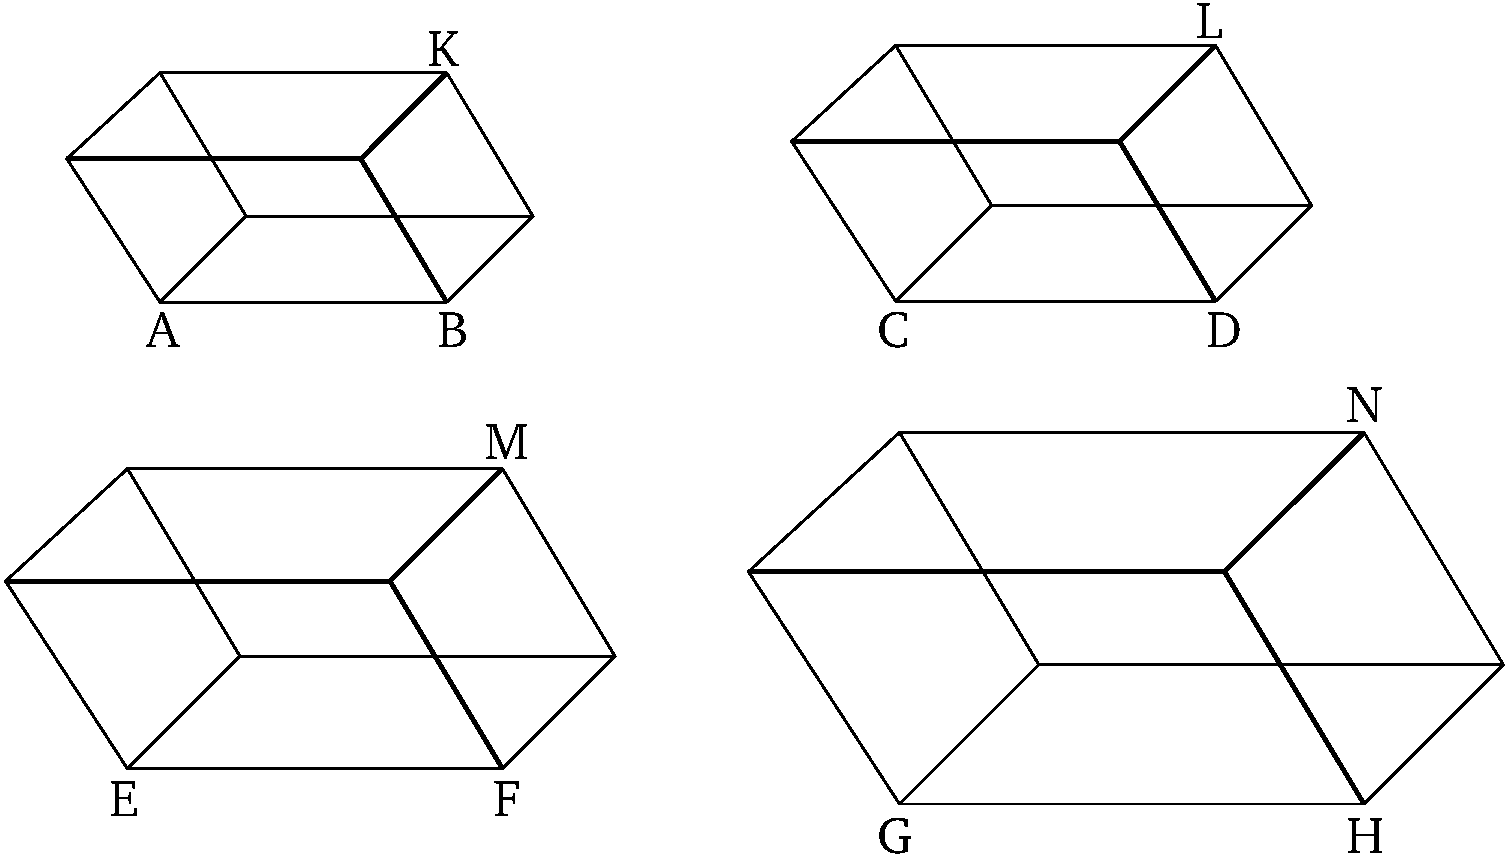
\includegraphics{Book11/fig37e.eps}}

Let $AB$, $CD$, $EF$, and $GH$, be four proportional
straight-lines, (such that) as $AB$ (is) to $CD$, so $EF$ (is) to $GH$. 
And let the similar, and similarly laid out, parallelepiped solids $KA$,
$LC$, $ME$ and $NG$ be described on $AB$, $CD$,
$EF$, and $GH$ (respectively). I say that as $KA$ is to $LC$, so
$ME$ (is) to $NG$.

For since the parallelepiped solid $KA$ is similar to $LC$, $KA$
thus has to $LC$ the cubed ratio that $AB$ (has) to $CD$ [Prop.~11.33]. So, for the same (reasons), $ME$ also has to
$NG$ the cubed ratio that $EF$ (has) to $GH$ [Prop.~11.33]. And since as $AB$
is to $CD$, so $EF$ (is) to $GH$, thus, also,  as $AK$ (is) to
$LC$, so $ME$ (is) to $NG$.

And so let solid $AK$ be to solid $LC$, as solid $ME$ (is) to $NG$.
I say that as straight-line $AB$ is to $CD$, so $EF$ (is) to $GH$.

For, again, since $KA$ has to $LC$ the cubed ratio that
$AB$ (has) to $CD$ [Prop.~11.33], and $ME$ also has to $NG$ the cubed ratio
that $EF$ (has) to $GH$ [Prop.~11.33], and as $KA$ is to $LC$, so $ME$
(is) to $NG$, thus, also, as $AB$ (is) to $CD$, so $EF$ (is) to $GH$.

Thus, if four straight-lines are proportional, and so on of
the proposition. (Which is) the very thing it was required to show.}
\end{Parallel}
{\footnotesize\noindent$^\dag$ This proposition assumes that if two
ratios are equal then the cube of the former is also equal to the cube of the
latter, and {\rm  vice versa}.}

%%%%
%11.38
%%%%
\pdfbookmark[1]{Proposition 11.38}{pdf11.38}
\begin{Parallel}{}{}
\ParallelLText{
\begin{center}
{\large \ggn{38}.}
\end{center}\vspace*{-7pt}

\gr{Ἐὰν κύβου τῶν ἀπεναντίον ἐπιπέδων αἱ πλευραὶ δίθα τμ\kern -.7pt  ηθῶσιν,
διὰ δὲ τῶν τομῶν ἐπίπεδα ἐκβληθῆ|, ἡ κοινὴ τομ\kern -.7pt  ὴ
τῶν ἐπιπέδων καὶ ἡ τοῦ κύβου διάμετροξ δίθα τέμνουσιν
ἀλλήλαξ.}

\epsfysize=2.3in
\centerline{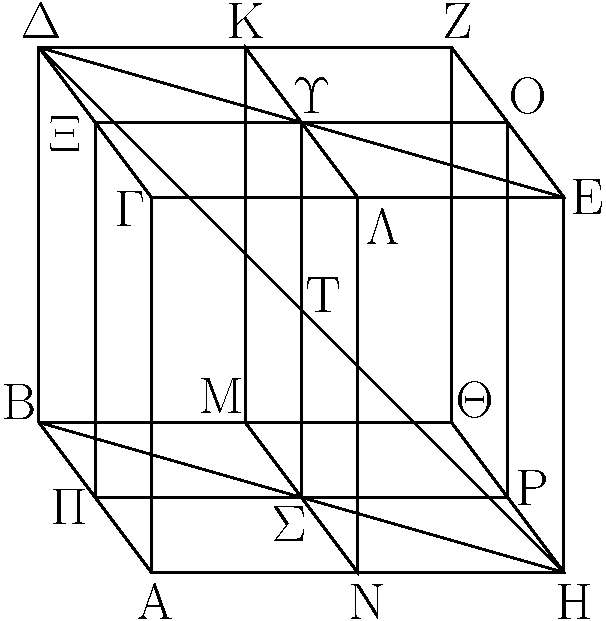
\includegraphics{Book11/fig38g.eps}}

\gr{Κύβου γὰρ τοῦ ΑΖ τῶν ἀπεναντίον ἐπιπέδων τῶν ΓΖ, ΑJ
αἱ πλευραὶ δίθα τετμ\kern -.7pt  ήσθωσαν κατὰ τὰ Κ, Λ, Μ, Ν, Χ, Π, Ο, Ρ
σημεῖα, διὰ δὲ τῶν τομῶν ἐπίπεδα ἐκβεβλήσθω τὰ ΚΝ, ΧΡ, κοινὴ
δὲ τομ\kern -.7pt  ὴ τῶν ἐπιπέδων >έστω ἡ ΥΣ, τοῦ δὲ ΑΖ κύβου διαγώνιοξ
ἡ ΔΗ. λέγω, <ότι >ίση ἐστὶν ἡ μὲν ΥΤ τῆ| ΤΣ, ἡ δὲ ΔΤ τῆ| ΤΗ.}

\gr{Ἐπεζεύθθωσαν γὰρ αἱ ΔΥ, ΥΕ, ΒΣ, ΣΗ. καὶ ἐπεὶ παράλληλόξ ἐστιν
ἡ ΔΧ τῆ| ΟΕ, αἱ ἐναλλὰχ γωνίαι αἱ ὑπὸ ΔΧΥ, ΥΟΕ >ίσαι
ἀλλήλαιξ εἰσίν. καὶ ἐπεὶ >ίση ἐστὶν ἡ μὲν ΔΧ τῆ| ΟΕ, ἡ
δὲ ΧΥ τῆ| ΥΟ, καὶ γωνίαξ >ίσαξ περιέθουσιν, βάσιξ >άρα ἡ ΔΥ
τῆ| ΥΕ ἐστιν >ίση, καὶ τὸ ΔΧΥ τρίγωνον τῶ| ΟΥΕ τριγώνῳ
ἐστὶν >ίσον καὶ αἱ λοιπαὶ γωνίαι ταῖξ λοιπαῖξ
γωνίαιξ >ίσαι; >ίση >άρα ἡ ὑπὸ ΧΥΔ γωνία τῆ| ὑπὸ ΟΥΕ
γωνίᾳ. διὰ δὴ τοῦτο εὐθεῖά ἐστιν ἡ ΔΥΕ. διὰ τὰ α\kern -.7pt  ὐτὰ
δὴ καὶ ΒΣΗ εὐθεῖά ἐστιν, καὶ >ίση ἡ ΒΣ τῆ| ΣΗ. καὶ ἐπεὶ
ἡ ΓΑ τῆ| ΔΒ >ίση ἐστὶ καὶ παράλληλοξ, ἀλλὰ ἡ ΓΑ καὶ τῆ|
ΕΗ >ίση τέ ἐστι καὶ παράλληλοξ, καὶ ἡ ΔΒ >άρα τῆ| ΕΗ >ίση τέ ἐστι καὶ
παράλληλοξ. καὶ ἐπιζευγνύουσιν α\kern -.7pt  ὐτὰξ εὐθεῖαι αἱ ΔΕ, ΒΗ; παράλληλοξ
>άρα ἐστὶν ἡ ΔΕ τῆ| ΒΗ. >ίση >άρα ἡ μὲν ὑπὸ ΕΔΤ γωνία
τῆ| ὑπὸ ΒΗΤ; ἐναλλὰχ γάρ; ἡ δὲ ὑπὸ ΔΤΥ τῆ| ὑπὸ ΗΤΣ.
δύο δὴ τρίγωνά ἐστι τὰ ΔΤΥ, ΗΤΣ τὰξ δύο γωνίαξ ταῖξ δυσὶ
γωνίαιξ >ίσαξ >έθοντα καὶ μίαν πλευρὰν μιᾶ| πλευρᾶ| >ίσην τὴν
ὑποτείνουσαν ὑπὸ μίαν τῶν >ίσων γωνιῶν τὴν ΔΥ τῆ| ΗΣ;
ἡμίσειαι γάρ εἰσι τῶν ΔΕ, ΒΗ; καὶ τὰξ λοιπὰξ πλευρὰξ ταῖξ
λοιπαῖξ πλευραῖξ >ίσαξ <έχει. >ίση >άρα ἡ μὲν ΔΤ τῆ| ΤΗ, ἡ δὲ ΥΤ τῆ| ΤΣ.}

\gr{Ἐὰν >άρα κύβου τῶν ἀπεναντίον ἐπιπέδων αἱ πλευραὶ δίθα τμ\kern -.7pt  ηθῶσιν,
διὰ δὲ τῶν τομῶν ἐπίπεδα ἐκβληθῆ|, ἡ κοινὴ τομ\kern -.7pt  ὴ
τῶν ἐπιπέδων καὶ ἡ τοῦ κύβου διάμετροξ δίθα τέμνουσιν
ἀλλήλαξ; <όπερ >έδει δεῖχαι.}}

\ParallelRText{
\begin{center}
{\large Proposition 38}
\end{center}

If the sides of the opposite planes of a cube are cut in half, and planes are produced through the pieces, then the common section of the (latter) planes and the diameter of the cube cut one another in half.

\epsfysize=2.3in
\centerline{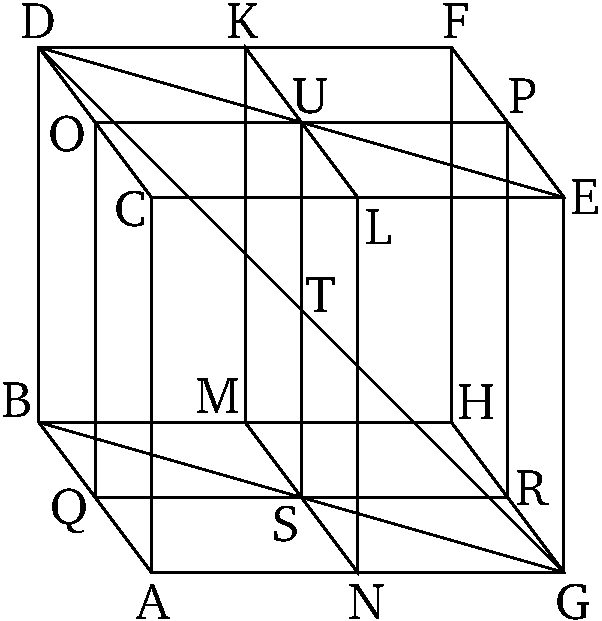
\includegraphics{Book11/fig38e.eps}}

For let the opposite planes $CF$ and $AH$ of the cube $AF$ be
cut in half at the points $K$, $L$, $M$, $N$, $O$, $Q$, $P$, and $R$. 
And let the planes $KN$ and $OR$ be produced through the
pieces. And let $US$ be the common section of the planes, and
$DG$ the diameter of cube $AF$. I say that $UT$ is equal to $TS$, and
$DT$ to $TG$.

For let $DU$, $UE$, $BS$, and $SG$ be joined. And since
$DO$ is parallel to $PE$, the alternate angles $DOU$ and $UPE$
are equal to one another [Prop.~1.29].
And since $DO$ is equal to $PE$, and $OU$ to $UP$, and they contain
equal angles, base $DU$ is thus equal to base $UE$, and triangle
$DOU$ is equal to triangle $PUE$, and the remaining angles (are) equal to
the remaining angles [Prop.~1.4]. Thus,
angle $OUD$ (is) equal to angle $PUE$. So, for  this (reason),
$DUE$ is a straight-line [Prop.~1.14].
So, for the same (reason), $BSG$ is also a straight-line, and $BS$ equal to
$SG$. And since $CA$ is equal and parallel to $DB$, but
$CA$ is also equal and parallel to $EG$, $DB$ is thus also equal and parallel 
to $EG$ [Prop.~11.9]. And the straight-lines
$DE$ and $BG$ join them. $DE$ is thus parallel to $BG$ [Prop.~1.33]. Thus, angle $EDT$ (is) equal to $BGT$.
For (they are) alternate [Prop.~1.29]. And (angle)
$DTU$ (is equal) to $GTS$ [Prop.~1.15]. So, $DTU$ and $GTS$ are two triangles having
two angles equal to two angles, and one side equal to one side---(namely),
that subtended by one of the equal angles---(that is), $DU$ (equal) to
$GS$. For they are halves of $DE$ and $BG$ (respectively).
(Thus), they will also have the remaining sides equal to the remaining
sides [Prop.~1.26]. Thus, $DT$ (is) equal
to $TG$, and $UT$ to $TS$.

Thus, if the sides of the opposite planes of a cube are cut in half, and planes are produced through the pieces, then the common section of the (latter) planes and the diameter of the cube cut one another in half. (Which is) the very thing it
was required to show.}
\end{Parallel}

%%%%
%11.39
%%%%
\pdfbookmark[1]{Proposition 11.39}{pdf11.39}
\begin{Parallel}{}{}
\ParallelLText{
\begin{center}
{\large \ggn{39}.}
\end{center}\vspace*{-7pt}

\gr{Ἐὰν >ῆ| δύο πρίσματα ἰσο"υψῆ, καὶ τὸ μὲν >έθῆ| βάσιν παραλληλόγραμμον, τὸ δὲ τρίγωνον, διπλάσιον δὲ >ῆ| τὸ παραλληλόγραμμον τοῦ τριγώνου, >ίσα >έσται τὰ πρίσματα.}

\epsfysize=1.2in
\centerline{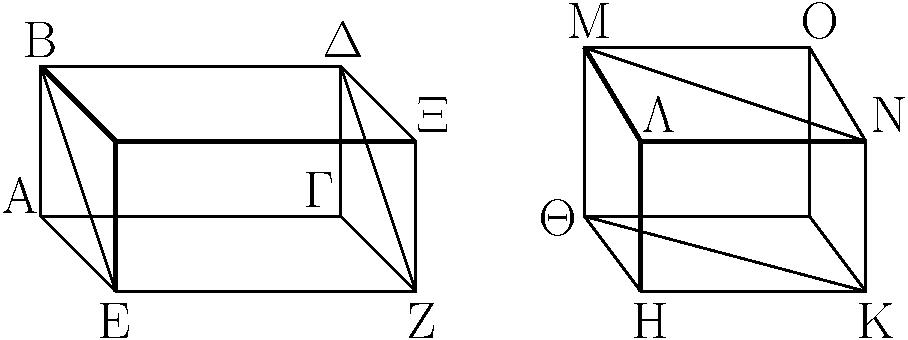
\includegraphics{Book11/fig39g.eps}}

\gr{>'Εστω δύο πρίσματα ἰσο"υψῆ τὰ ΑΒΓΔΕΖ, ΗJΚΛΜΝ, καὶ τὸ
μὲν ἐθέτω βάσιν τὸ ΑΖ παραλληλόγραμμον, τὸ δὲ τὸ ΗJΚ τρίγωνον,
διπλάσιον δὲ >έστω τὸ ΑΖ παραλληλόγραμμον τοῦ ΗJΚ τριγώνου;
λέγω, <ότι >ίσον ἐστὶ τὸ ΑΒΓΔΕΖ πρίσμα τῶ| ΗJΚΛΜΝ
πρίσματι.}

\gr{Συμπεπληρώσθω γὰρ τὰ ΑΧ, ΗΟ στερεά. ἐπεὶ διπλάσιόν ἐστι τὸ ΑΖ
παραλληλόγραμμον τοῦ ΗJΚ τριγώνου, >έστι δὲ καὶ τὸ JΚ παραλληλόγραμμον διπλάσιον τοῦ ΗJΚ τριγώνου, >ίσον >άρα ἐστὶ
τὸ ΑΖ παραλληλόγραμμον τῶ| JΚ παραλληλογράμμῳ. τὰ δὲ ἐπὶ
>ίσων βάσεων >όντα στερεὰ παραλληλεπίπεδα καὶ
ὑπὸ τὸ α\kern -.7pt  ὐτὸ <ύψοξ >ίσα ἀλλήλοιξ ἐστίν; >ίσον >άρα ἐστὶ
τὸ ΑΧ στερεὸν τῶ| ΗΟ στερεῶ|. καί ἐστι τοῦ μὲν ΑΧ στερεοῦ
<ήμισυ τὸ ΑΒΓΔΕΖ πρίσμα, τοῦ δὲ ΗΟ στερεοῦ <ήμισυ τὸ
ΗJΚΛΜΝ πρίσμα; >ίσον >άρα ἐστὶ τὸ ΑΒΓΔΕΖ πρίσμα τῶ|
ΗJΚΛΜΝ πρίσματι.}

\gr{Ἐὰν >άρα >ῆ| δύο πρίσματα ἰσο"υψῆ, καὶ τὸ μὲν >έθῆ| βάσιν παραλληλόγραμμον, τὸ δὲ τρίγωνον, διπλάσιον δὲ >ῆ| τὸ παραλληλόγραμμον τοῦ τριγώνου, >ίσα >έστὶ τὰ πρίσματα; <όπερ
>έδει δεῖχαι.}}

\ParallelRText{
\begin{center}
{\large Proposition 39}
\end{center}

If there are two equal height prisms,
and one has a parallelogram, and the other a triangle,  (as a) base, 
and the parallelogram is double the triangle, then the prisms will be equal.

\epsfysize=1.2in
\centerline{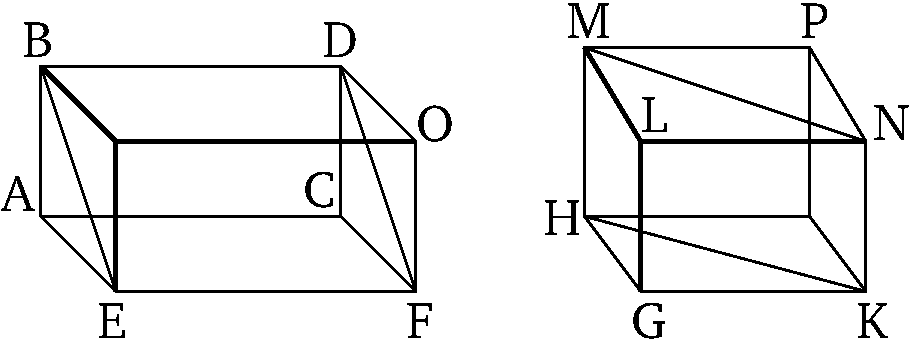
\includegraphics{Book11/fig39e.eps}}

Let $ABCDEF$ and $GHKLMN$ be two equal height prisms, and
let the former have the parallelogram $AF$, and the latter the
triangle $GHK$, as a base. And let parallelogram $AF$ be twice
triangle $GHK$. I say that prism $ABCDEF$ is equal to prism
$GHKLMN$.

For let the solids $AO$ and $GP$ be completed. 
Since parallelogram $AF$ is double triangle $GHK$, and parallelogram
$HK$ is also double triangle $GHK$ [Prop.~1.34],
parallelogram $AF$ is thus equal to parallelogram $HK$. And parallelepiped
solids which are on equal bases, and (have) the same height, are equal
to one another [Prop.~11.31]. Thus, solid
$AO$ is equal to solid $GP$.  And prism $ABCDEF$ is half of solid
$AO$, and prism $GHKLMN$ half of solid $GP$ [Prop.~11.28]. Prism $ABCDEF$ is thus equal to prism $GHKLMN$.

Thus, if there are two equal height prisms,
and one has a parallelogram, and the other a triangle,  (as a) base, 
and the parallelogram is double the triangle, then the prisms are equal.
(Which is) the very thing it was required to show.}

\ParallelPar
\end{Parallel}